\documentclass[a4paper,12pt,twoside,openany]{scrbook}
\usepackage[ngerman]{babel}
\usepackage[utf8]{inputenc}
\usepackage{amsfonts}
\usepackage{amsmath}
\usepackage[T1]{fontenc}
\usepackage{graphicx}
\usepackage{srcltx}
\usepackage{multicol}
%\usepackage{wrapfig}
\usepackage{subfigure}

%\pagestyle{myheadings}

%\usepackage{hyperref}

\usepackage[colorlinks=true,linkcolor=black,citecolor=black,bookmarksnumbered=true,breaklinks=true,pdfstartview=FitH]{hyperref}

% Schriftart: Palatino
%\usepackage{mathpazo}
%\linespread{1.05}


	%Index
\usepackage{makeidx}
\makeindex
\newcommand{\ind}[1]{#1 \index{#1} }

\author{Michael Kopp}
\date{1. Auflage}
\title{Physik\\der Oberstufe}

\begin{document}

\maketitle

\addchap*{Dieses Buch}

\begin{quote}
Hier präsentiere ich Ihnen stolz mein Physik-Script. Für die Oberstufe habe ich vor jeder anstehenden Klausur für mich eine Zusammenfassung erstellt -- und weil ich diese Zusammenfassungen in \LaTeX\ tippte, konnte ich sie für meine Mitschüler verfügbar machen. So bekam ich nicht nur ein gutes Feedback, sondern unser Kurs wohl teilweise einen besseren Schnitt\dots

Ich habe das Werk in mehrere große Themen aufgeteilt, die mehr oder weniger unabhängig voneinander dastehen. Was mir aber wichtig ist, ist die Verknüpfung des Wissens bzw. der Informationen \emph{innerhalb} der Unterabschnitte. So wird man auf zahlreiche Referenzen und Verweise stoßen, die einfach zeigen sollen, dass ein ähnlicher Inhalt schon unter einem anderen Gesichtspunkt abgehandelt worden war -- hier besteht also eine Inhaltliche Verknüpfung.
Darüber hinaus endet dieses Buch mit einem seitenlangen Index, in dem man die wichtigsten Begriffe finden kann und die dazugehörige Seite sieht.

Wie oben schon angedeutet: Ich habe all das hier am PC getippt -- und zwar sehe ich beim Schreiben nur schlichte \texttt{Courier-Schrift}. Besonders bei Formeln können sich da Fehler eingeschlichen haben. Aber auch sonst wimmelt diese Buch vermutlich von kleineren bis übermittelgroßen Fehlern. Manchmal habe ich auch versucht, Sachverhalte \emph{besser} als unser Buch bzw. unser Lehrer zu erklären. Dabei sind manchmal etwas seltsame und anspruchsvolle Gedankengänge entstanden, und ich hoffe, ich konnte diese vernünftig entwickeln, sodass der leser auch etwas davon hat. Hier findet der interessierte Leser auch Formeln und Details, die im Unterricht (zumindest bei uns) keinen Platz hatten, von denen ich aber denke, dass sie interessant sein könnten und das Thema abrunden. In diesem Werk wurden diejenigen meiner Praktika aufgenommen, die lehrreich sind; so haben es eben nur wenige geschafft, hier aufgenommen zu werden...

Insgesamt denke ich, dass man mit diesem Buch ganz vernünftig aufs Abi lernen könnte -- mir blieb das erspart, weil im entscheidenden Moment meine Affinität zur Chemie überwog.

Auf jeden Fall bitte ich herzlich darum, sich nicht allzusehr über die Fehler aufzuregen, sondern sich stattdessen über den richtigen Rest zu freuen. Viel Spaß bei der Lektüre.

\begin{flushright}
     Michael Kopp, im August 2008
\end{flushright}


\end{quote}



\newpage


\tableofcontents

\sloppy

\part{E-Feld}
		\chapter {Definitionen zu Strom}
Strom\index{Strom} kann dann fließen, wenn ein geschlossener \textbf{\textit{Stromkreis}}\index{Stromkreis} vorliegt. Dabei transportieren Elektronen (\(e^{-}\)) elektrische Energie von einer \textit{Strom-} bzw. \textit{Spannungsquelle} zu einem Verbraucher, der sie dann in andere Energieformen umsetzen kann. 

\subsubsection{Spannung: } \index{Spannung}
Ein Maß dafür, wie Viel Energie ein einzelnes Elektron dabei transportiert ist die Spannung \(U\) in Volt \(V\)
	\begin{equation}
	U = \frac{W}{Q} ~~~~~~~~~~~~~~ [U]=\frac{J}{C}=V
	\label{def_U}
	\end{equation}
mit \(W\) als transportierter Energie in Joule \(J\) und \(Q\) als bewegter Ladung in Coulomb \(C\).

\subsubsection{Potential: } Eigentlich handelt es sich bei Spannung um eine \textit{Potentialdifferenz}\index{Potential}\index{Spannung}. Jeder Punkt in einem Elektrischen Stromkreis hat ein Potential \(\varphi\). Es stellt dar, wie viel Energie pro Ladung frei wird, wenn zwischen einem Punkt \(P_1\) (einem beliebigen Punkt) und \(P_0\) (der Erdung\index{Erdung}\footnote{Statt der Erdung kann auch ein anderer, beliebiger Punkt \(P_0\) im Stromkreis gewählt werden, solange es immer der selbe Punkt ist.}) eine Leitung hergestellt wird. Das Potential bezeichnet man dann mit \(\varphi_{01}\). Ein weiterer Punkt \(P_2\) hat nun ein Potential \(\varphi_{02}\) in Bezug auf die Erdung und ein Potential \(\varphi_{12}\) im Bezug auf Punkt \(P_1\). \(\varphi_{12}\) bezeichnet man auch als \textit{Spannung} zwischen \(P_1\) und \(P_2\). Es gilt also:
	\begin{equation}
	U_{A~zu~B} = \varphi_{A~zu~Erdung} - \varphi_{B~zu~Erdung} = \Delta\varphi
	\label{def_potential}
	\end{equation}
Sowohl das Potential \(\varphi\), als auch die Spannung \(U\) haben die Einheit Volt \(V\).\index{Volt}

\subsubsection{Stromstärke: }
Ein Maß dafür, wie viele Elektronen in einer bestimmten Zeit durch den Stromkreis fließen ist die Stromstärke \(I\) in Ampère \(A\)\index{Stromstärke}\index{Ampère}
	\begin{equation}
	I = \frac{Q}{t} ~~~~~~~~~~~~~~ [I]=\frac{C}{s}
	\label{def_I}
	\end{equation}
mit \(t\) als Zeit in Sekunden \(s\).

\subsubsection{Leistung: }\index{Leistung!Elektrische}
Kombiniert man Spannung und Stromstärke (also Gleichungen (\ref{def_U}) und (\ref{def_I})), so kann man die Elekrtische Leistung \(P\) in Watt \(W\) errechnen: 
	\begin{equation}
	P = I \cdot U = \frac{W}{Q} \cdot \frac{Q}{t} = \frac{W}{t} ~~~~~~~~~~~~~~ [P] = \frac{J}{s}=W
	\label{def_P}
	\end{equation}
	
	
		\chapter{Widerstand}
		
		%\begin{wrapfigure}{r}{0.4\textwidth}
		\begin{figure}
		\centering
		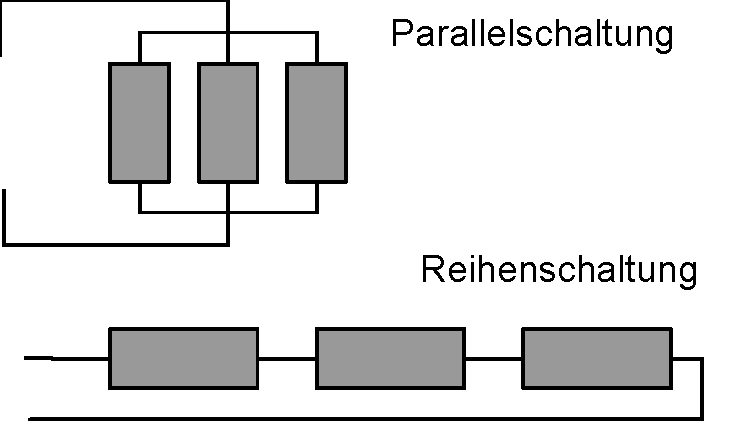
\includegraphics[width=0.6\textwidth]{mat/schaltungen}
		\caption{Arten von Schalverbänden}
		\label{img_schaltungen}
		%\end{wrapfigure}
		\end{figure}
		
Ein Widerstand\index{Widerstand!Elektrischer} ist ein technisches Bauteil, das elektrische Energie in Wärmeenergie unsetzt. In einen Stromkreis eingebaut sorgt es dafür, dass ein Teil der von der Quelle abgegebenen Leistung für einen Verbraucher nicht nurzbar ist, da sie schon vorher am Widerstand in Wärme umgesetzt wurde.\footnote{Im weitesten Sinne ist jeder nicht supraleitende Leiter ein Widerstand}

Man unterscheidet zwischen \textit{parallel} und \textit{in Reihe}\index{Parallelschaltung}\index{Reihenschaltung} geschalteten Widerständen (siehe Abb. \ref{img_schaltungen} auf S. \pageref{img_schaltungen}). Während ein Widerstand, der parallel zu einem Verbraucher geschaltet ist, die selbe Spannung \(U\) abbekommt wie der Verbraucher, wird ein Widerstand, der in Reihe zum Verbraucher geschaltet wird von dem selben Strom\footnote{also der selbe Stromstärke \(I\)} durchflossen.

Für Ohmsche Widerstände gilt dabei das \textsc{Ohm}'sche Gesetz:\index{Ohm'sches Gesetz}
	\begin{equation}
	R = \frac{U}{I} = \frac{\frac{W}{Q}}{\frac{Q}{t}} = \frac{W \cdot t}{Q^2} ~~~~~~~~~~~~~~ [R] = \frac{\frac{W}{Q}}{\frac{Q}{t}} = \frac{J \cdot s}{C^2} = \Omega
	\label{def_R}
	\end{equation}
Es besagt, dass bei sogenannten \textit{ohmschen} Widerständen\index{Widerstand!Ohm'scher} sich Stromstärke zur Spannung am Widerstand bzw. Leiter proportional zueinander verhalten. Die Proportionalitätskonstannte \(R\) stellt den Widerstand in Ohm \(\Omega\) dar. 

Aus einem Verbund an Widerständen lässt sich ein \textit{Ersatzwiderstand}\index{Ersatzwiderstand} \(R_{ersatz}\) berechnen. Man kann sich dabei vorstellen, dass man die Widerstände, die man zu seiner Berechnung heranziehr, entfernt, und dafür ein Bauteil einsetzt, das den Widerstand hat, wie die einzelnen Bauteile zusammen. Dabei muss man bei der Summation der Widerstände berücksichtigen, ob sie in Reihe oder parallel geschaltet sind; Für den Ersatzwiderstand in einer Reihenschaltung ergibt sich:
	\begin{equation}
	R_{Ersatz} = R_1 + R_2 + R_3 + ...
	\label{Rers_reihe}
	\end{equation}
Für parallel geschaltete Widerstände ergibt sich jedoch:
	\begin{equation}
	R_{Ersatz} = \frac{1}{\frac{1}{R_1} + \frac{1}{R_2} + \frac{1}{R_3} + ....}
	\label{Rers_parallel}
	\end{equation}	


%		\part{das Elekrtische Feld "`\textit{E-Feld}"'}	

		\chapter{Feldlinienmodell}

Zwischen zwei Ladungen \(Q_1\) und \(Q_2\) besteht immer ein E-Feld. Deshalb bezeichnet man sie als \textit{felderzeugende Ladungen}.\footnote{Felderzeugende Ladungen erhalten ein großes \(Q\), Probeladungen (die kleiner sind als die felderzeugenden) erhalten ein kleines \(q\).}\index{Felderzeugende Ladung}\index{Feldlinien}

Ein E-Feld ist derjenige Bereich, in dem auf ein elektrisch geladenes Teilchen -- mit der Probeladung\index{Probeladung} \(q\)  (positiv oder negativ) -- eine elektrische Kraft ausgeübt wird, die von Anziehungen oder Abstoßungen der felderzeugenden Ladungen herrühren.

Aufgrund des E-Feldes führt eine Probeladung folglich Bewegungen innerhalb des Feldes aus. Bahnen, auf denen sich eine solche Probeladung bewegen, bezeichnet man als \textit{Feldlinien}. In der Darstellung besteht die Konvention, dass man den Weg eines positiv geladenen Probeteilchens einträgt, also den Feldlinien mittels Pfeilspitzen die Richtung zuweist, die eine positive Ladung nehmen würde. Die Feldlinien laufen von einer positiven Felderzeugenden Ladung \(Q_1\) zu einer negativen \(Q_2\). Sie stehen jeweils auf der Oberfläche der Ladungsträger und kreuzen sich nicht. Für Darstellungen gilt, dass die Kräfte auf ein Probeteilchen umso stärker sind, je dichter die Feldlinien an dieser Stelle sind.

Es kann dazu kommen, dass E-Felder abgeschirmt werden -- beispielsweise beim \textsc{Faraday}'schen Käfig. Hier besteht innerhalb eines von Leitern eingeschlossenen Bereichs kein E-Feld, rundherum dagegen schon.

		\chapter{Elektrische Feldstärke}
		
		\section{Kraft auf Ladungsträger}
		\label{F_auf_q}
Die Kraft auf eine Probeladung wirkt tangential zu den Feldlinien. Diese Kraft \(F_{el}\) ist Proportional zu der elektrischen Ladung \(q\) des Teilchens. Verlaufen Feldlinien in einem Bereich gerade, parallel und im selben Abstand voneinander, so spricht man in diesem Bereich von einem \textit{homogenen} E-Feld\index{E-Feld!Homogenes}.\footnote{Es tritt beispielsweise (nährungsweise) zwischen zwei elektrisch gelandenen parallelen Platten auf.} In diesem ist die Elektrische Feldstärke \(\vec{E}\) konstant\footnote{in Betrag und Richtung}. \\
Normalerweise sind E-Felder \textit{inhomogen}.
	\begin{equation}
	\vec{E} = \frac{\vec{F_{el}}}{q} ~~~~~~~~~~~~~~ [\vec{E}] = \frac{N}{C} = \frac{\frac{J}{m}}{C} = \frac{V}{m}
	\label{def_E}
	\end{equation}
wobei \(\vec{E}\) die Elektrische Feldstärke des Feldes ist.


		\section{Distanzen im E-Feld}
Um Ladungen in einem homogenen E-Feld der Feldstärke \(E\) parallel zu den Feldlinien zu bewegen, benötigt\footnote{bzw. wird frei; bewegt man eine positive Ladung mit den Feldlinien, wird Energie frei -- in anderen Fällen entsprechend} 
man die Energie \(W\). Diese ist proportional zu der Strecke \(l\) parallel der Feldlinien, sowie der Ladung \(q\) des Teilchens. Es gilt dabei: 
	\begin{equation}
	W = q \cdot E \cdot l ~~~~~~~~~~~~~~ [W] = C \cdot \frac{N}{C} \cdot m = Nm = J
	\label{W_kondensator}
	\end{equation}
Benutzt man nun Formel \ref{def_U}, so gilt:
	\begin{equation}
	U = E \cdot l
	\label{U=El}
	\end{equation}
Interpretiert man das Ergebnis nach Formel \ref{def_potential}, so gilt folgendes: Zwischen den Punkten \(P_{1}\) und \(P_2\) in einem E-Feld liegt immer die Spannung \(\Delta\varphi = U_{1~zu~2} = E \cdot l\), wobei man die Strecke \(l\) nur in Richtung der Feldlinien messen muss.

Das bedeutet widerrum, dass man Ladungen problemlos senkrecht zu den Feldlinien bewegen kann. Diese Linien\footnote{bzw. im Raum diese Flächen} bezeichnet man als \textit{Äquipotentialflächen}.



		\chapter{Kondensator}

Im Grunde besteht ein \emph{Kondensator}\index{Kondensator} aus zwei Metallplatten, die durch ein \emph{Dielektrikum}\index{Dielektrikum} voneinander getrennt sind. Schließt man die Pole einer Spannungsquelle an einen Kondensator an, so wird er aufgeladen und kann elektrische Energie speichern und später wieder abgeben. Für Kondensatoren gibt es zahlreiche Aufbaumöglichkeiten.



		\section{Stärke des E-Felds im Kondensator}
Das Homogene E-Feld im Kondensator\index{E-Feld!Homogenes} kann man leicht ausrechnen. Durch Umformung von Formel \ref{U=El} kommt man für einen Kondensator, an dem die Spannung \(U\) zwischen zwei Platten, die sich im Abstand \(d\) voneinander entfernt befinden, anliegt,  auf:
	\begin{equation}
	E = \frac{U}{d}
	\label{E_kondensator}
	\end{equation}


		\section{Zusammenhang mit felderzeugenden Ladungen}	
Auf Kondensatorplatten der Fläche \(A\) sind die felderzeugenden Ladungen \(Q\) gleichmäßig auf der Außenseite verteilt\footnote{Es geht dabei um die Ladung \textit{einer} Platte}. Der Quotient \(\sigma\) gibt an, wie groß die Ladung auf einer bestimmten Fläche ist:
	\begin{equation}
	\sigma = \frac{Q}{A} ~~~~~~~~~~~~~~ [\sigma] = \frac{C}{m^2}
	\label{def_sigma}
	\end{equation}	
Diese \textit{Flächenladungsdichte} \(\sigma\) auf den Kondensatorplatten steht in direktem Zusammenhang mit der Feldstärke \(E\) zwischen den Platten. Es git nämlich:
	\begin{equation}
	E = \frac{\sigma}{\varepsilon_0 \cdot \varepsilon_r} ~~~~~~~~~~~~~~ [E] = \frac{\frac{C}{m^2}}{\frac{C}{Vm} \cdot 1} = \frac{V}{m}
	\end{equation}
Dabei ist \(\varepsilon_0\) die Elektrische Feldkonstante mit \(\varepsilon_0 \approx 8,85 \cdot 10^{-12} \frac{C}{Vm}\) und \(\varepsilon_r\) die Dielektritätszahl (\(\rightarrow\) Kapitel \ref{kap_epsilon_r})  mit \(\varepsilon_r \approx 1\) für Luft.


		\section{Kapazität}
Die Kapazität \(C\)\index{Kapazität} eines Kondensators gibt an, wie viel Ladung \(Q\) bei einer bestimmten Spanung \(U\) gespeichert werden kann. Sie ist deshalb definiert als der Quotient von Ladung \(Q\) und Spannung \(U\):
	\begin{equation}
	C = \frac{Q}{U} ~~~~~~~~~~~~~~ [C] = \frac{C}{V} = F
	\label{def_C}
	\end{equation}
Dabei ist \(C\) die Kapazität in Farad \(F\). 

Die Kapazität eines Plattenkondensators mit homogenem E-Feld kann darüber hinaus noch folgendermaßen berechnet werden:
	\begin{equation}
	C = \varepsilon_0 \cdot \varepsilon_r \cdot \frac{A}{d} ~~~~~~~~~~~~~~ [C] = \frac{C}{Vm} \cdot \frac{m^2}{m} = \frac{C}{V} = F
	\label{C_kondensator}
	\end{equation}
Wobei \(A\) die Oberfläche einer Platte in \(m^2\) und \(d\) der Abstand der Platten in \(m\) darstellt.


		\subsection{Dielektrizitätszahl}
		\label{kap_epsilon_r}
Die Dielektrizitätszahl \(\varepsilon_r\)\index{Dielektrizitätszahl} gibt an, um welchen Faktor sich die Kapazität verändert, wenn ein \textit{Dielektrikum}\footnote{Materie im Kondensator, durch die das E-Feld geht} eingeführt wird. Es handelt sich dabei um eine Materialkonstante die vom Stoff anbängt. Es gilt dabei:
	\begin{equation}
	\varepsilon_r = \frac{C_{Dielektrikum}}{C_{Vakuum}}
	\label{def_epsilon_r}
	\end{equation}
Weiter gilt als gute Nährung \(C_{Vakuum} \approx C_{Luft}\) 	


		\section{Schaltungen von Kondensatoren}
Schaltet man Kondensatoren parallel (\(\rightarrow\) Abb. \ref{img_schaltungen}), so kann man als \textit{Ersatzkapazität} die Kapazitäten der einzelnen Kondensatoren Addieren:
	\begin{equation}
	C_{Ersatz} = C_1 + C_2 + C_3 + ...
	\end{equation}
Man kann sich dabei vorstellen, das die Platten der Kondensatoren, die den selben Plattenabstand haben, seitlich aneinander angefügt werden und sich somit eine Fläche ergibt, die sich aus allen Teilflächen addiert. Betrachtet man nun Formel \ref{C_kondensator}, so ist ersichtlich, wieso man so rechnet.

Schaltet man die Kondensatoren dagegen in Reihe, so muss man zum Berechnen der Ersatzkapazität folgendermaßen vorgehen:
	\begin{equation}
	C_{Ersatz} = \frac{1}{\frac{1}{C_1} + \frac{1}{C_2} + \frac{1}{C_3} + ....}
	\end{equation}
Hierbei ist es so, als würden sich die Plattenabstände aller Kondensatoren mit den Selben Plattenflächen addieren. Aus Formel \ref{C_kondensator} ist dieses Vorgehen wieder ersichtlich.


		\section{Speichern von Energie im Kondensator}	
Ein Kondensator kann an einer Spannungsquelle aufgeladen werden. Diese kann dann abgetrennt werden. Da das E-Feld zwischen den Kondensatorplatten von den Ladungen \(Q_{1,2}\) auf den Platten kommt, und diese Ladungen nicht abfließen können, bleibt das E-Feld weiterhin erhalten. In ihm ist nun Energie gespeichert\footnote{beispielsweise kann ein geladenes Teilchen immernoch darin bewegt werden \(\rightarrow\) Formel \ref{W_kondensator} oder sie kann einen Verbraucher dazu bringen, Arbeit zu verrichten}.

Nach Formel \ref{def_U} kann man die gespeicherte Energie des Kondensators berechnen, indem man Spannung \(U\) und Ladung \(Q\) multipliziert. Da die Spannung dabei nicht konstant ist, sondern sich proportional zur Ladung verhält (\(\rightarrow\) Formel \ref{def_C}), berechnet man dazu das Integral:
	\begin{equation}
	W = \int^{U_B}_{U_A} C\cdot U ~dU = \left[ \frac{1}{2} \cdot C \cdot U^2 \right]^{U_B}_{U_A} = \frac{1}{2} \cdot C \cdot U^2_B - \frac{1}{2} \cdot C \cdot U_A^2
	\label{W_speicherung}
	\end{equation}
Das Integral ließe sich mit Formel \ref{def_C} umschreiben:
	\begin{equation}
	W = \int^{U_B}_{U_A} C\cdot U ~dU = \left[ \frac{1}{2} \cdot Q \cdot U \right]^{U_B}_{U_A}
	\end{equation}
Wird ein Dielektrikum\index{Dielektrikum} eingeführt, so erhöht sich die Speicherkapazität des Kondensators um den Faktor \(\varepsilon_r\), da sich die Kapazität ja genauso erhöht (\(\rightarrow\) Kapitel \ref{kap_epsilon_r}).


		\subsection{Energiespeicherort}
Die Energie, die der Kondensator speichert, wird in dem Raum gespeichert, den das E-Feld ausfüllt. Formel \ref{W_speicherung} kann man umformen (der Einfachheit halber sei \(U_A = 0\) und \( U_B = U\)):
	\begin{equation}
	W = \frac{1}{2} \cdot Q \cdot U = \frac{1}{2} \cdot C \cdot U^2 = \frac{1}{2} \cdot \varepsilon_0 \cdot \varepsilon_r \cdot \frac{A}{d} \cdot E^2 \cdot d^2 =  \frac{1}{2} \cdot \varepsilon_0 \cdot \varepsilon_r  \cdot E^2 \cdot V
	\end{equation}
Wobei \(V\) das Volumen des vom homogenen E-Feld durchsetzten Raum im \(m^3\) darstellt.	


		\chapter{Teilchen im E-Feld}
		
		\section{Beschleunigung}
		
		%\begin{wrapfigure}{l}{0.23\textwidth}
		\begin{figure}
		\centering
		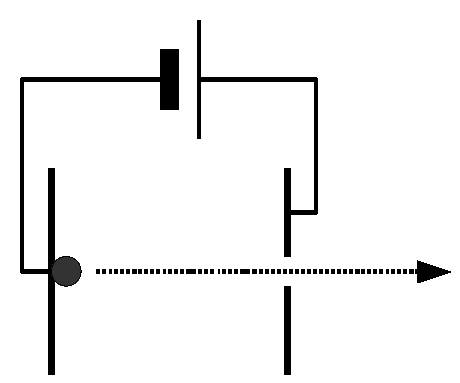
\includegraphics[width=0.6\textwidth]{mat/beschleunigung}
		\caption{negatives Teilchen beschleunigt}
		\label{img_beschleunigung}
		%\end{wrapfigure}
		\end{figure}
Ein geladenes Teilchen kann mit einem E-Feld beschleunigt werden. Aufbau siehe Abb. \ref{img_beschleunigung} auf S. \pageref{img_beschleunigung}. Dazu ist in einer der Kondensatorplatten ein Loch. Das Teilchen wird zur gegenüberliegenden Platte gebracht und diese wird gleichnamig zum Teilchen geladen -- die Platte mit Loch entsprechend ungleichnamig -- indem eine Spannung \(U\) angelegt wird.

Von der Platte ohne Loch wird das Teilchen also abgestoßen und von der mit Loch angezogen. Da das Teilchen dabei möglichst den kompletten Kondensator durchfliegt, nimmt es nach Formel \ref{def_U} die Energie \(W = U \cdot q \) auf. Diese Energie wird bei dem Teilchen vollständig in Bewegungsenergie umgewandelt und somit ergibt sich mit der Formel für kinetische Energie:
	\begin{equation}
	v = \sqrt{\frac{2 \cdot W}{m}} = \sqrt{\frac{2 \cdot U \cdot q}{m}} ~~~~~~~~~~~~~~ [v] = \sqrt{\frac{\frac{J}{C}\cdot C}{kg}} = \sqrt{\frac{Nm}{kg}} = \frac{m}{s}
	\end{equation}
Dabei ist \(m\) die Masse des Teilchens.

		\section{Ablenkung}
		\begin{figure}
		\centering
		%\begin{wrapfigure}{r}{0.23\textwidth}
		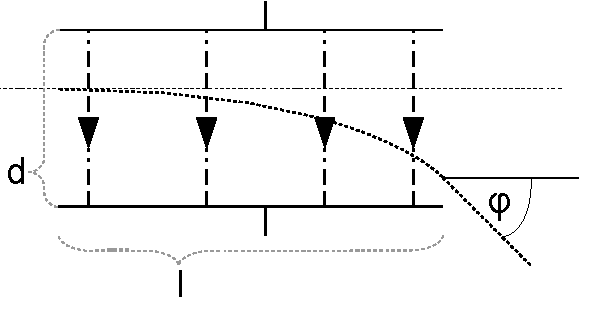
\includegraphics[width=0.6\textwidth]{mat/ablenkung}
		\caption{Teilchen wird abgelenkt}
		\label{img_ablenkung}
		%\end{wrapfigure}
		\end{figure}
Aus Kapitel \ref{F_auf_q} wissen wir, dass ein geladenes Teilchen im E-Feld eine Kraft erfährt, die von seiner Ladung abhängt (\(\rightarrow\) Formel \ref{def_E}). Bewegt sich nun ein Teilchen zwischen zwei Kondensatorplatten, zwischen denen eine Spannung \(U\) anliegt, durch, so befindet es sich in einem E-Feld, von dem es abgelenkt wird. Siehe dazu Abb. \ref{img_ablenkung} auf S. \pageref{img_ablenkung}.

Zu der anfänglichen Bewegung \(v_0\) kommt im Kondensator noch eine weitere, gleichmäßig beschleunigte Bewegung \(v_1\) -- abhängig von der Ladung \(q\) und der Masse \(m\) des Teilchens -- in Richtung einer der beiden Platten\footnote{positiv geladene Teilchen werden in Richtung der negativ geladenen Platte abgelenkt und entsprechend} hinzu. Für die Distanz \(\Delta y\), die das Teilchen in Richtung einer Platte abgelenkt wurde gilt:
	\begin{equation}
	\Delta y = \frac{E \cdot q}{2 \cdot m} \cdot t^2 = \frac{U \cdot q}{2 \cdot d \cdot m} \cdot t^2 = \frac{U \cdot q}{2\cdot d \cdot m \cdot v_0^2} \cdot ( \Delta x)^2
	\label{ablenkung_kondensator}
	\end{equation}
Dabei ist \(E\) die Feldstärke des E-Feldes zwischen den Kondensatorplatten, \(U\) die Spannung zwischen den beiden Platten, \(d\) der Abstand zwischen den beiden Platten und \(\Delta x\) die Distanz in Richtung der ursprünglichen Bewegung, die das Teilchen schon im Kondensator hinter sich gebracht hat. 

Das Teilchen folgt im Kondensator also einer Parabelförmigen Flugbahn.


		\subsection{Weiterflug}
Verlässt das Teilchen dann den Kondensator, nachdem es ihn auf der Länge \(l\) (parallel zu den Platten gemessen) durchflogen hat, so setzt sich seine Bewegung aus zwei gleichförmigen Bewegungen zusammen -- \(v_0\) und \(v_1\), da nun keine Beschleunigenden Kräfte mehr auf sie wirken. Es ergibt sich dadurch eine Gesamtgeschwindigkeit \(v_{ges}\) von:
	\begin{equation}
	v_{ges} = \sqrt{v_0^2 + v_1^2}
	\end{equation}
Mit dieser Geschwindigkeit setzt das Teilchen seinen Weg fort. Um die Richtung zu ermitteln, leitet man Formel \ref{ablenkung_kondensator} ab. Den Winkel \(\varphi\) zwischen der Neuen Flugbahn \(\vec{v}_{ges}\) und der alten \(\vec{v}_0\) erhält man mithilfe dieser Ableitung:
	\begin{equation}
	\varphi = \tan \left ( \frac{U \cdot q \cdot l}{d \cdot m \cdot v_0^2} \right )
	\end{equation}
Dabei ist \(U\) die Spannung, die zwischen den Kondensatorplatten anligt, \(m\) die Masse des Teilchens, \(q\) seine Ladung und \(v_0\) die Geschwindigkeit, mit der es parallel zu den Platten ankam.


% \part{Anhang}
%
% \chapter{Definitionen, Größen}
%
% \begin{description}
% 	\item[\(\varepsilon_0\)] Elektrische Feldkonstante \(\varepsilon_0 \approx 8,85 \cdot 10^{-12} \frac{C}{Vm}\)
% \end{description}

%\cleardoublepage

\part{B-Feld}

		\chapter{Die Magnetische Flussdichte}

Die Magnetische Flussdichte\index{Magnetische Flussdichte} \(B\) ist ein Vektor, mit dessen Hilfe sich berechnen lässt, wie sich ein Magnetisches Feld auf seine Umwelt auswirkt.

		\section{Draht im Magnetfeld} \label{sec1}

Die Magnetische Flussdichte \(B\) gibt an, welche Kraft \(F\) ein Leiter mit der wirksamen Länge\footnote{es ist nur die Länge entscheident, die senkrecht zu den magnetischen Feldlinien steht. Schließt der Draht also den Winkel \(\alpha\) mit den Feldlinien ein, so muss seine wirksame Länge \(s\) berechnet werden mit \(s = s_r \cdot sin(\alpha)\), wobei \(s_r\) die reale Länge des Drahtes ist}~\(s\), der von einem Strom der Stärke \(I\) durchflossen wird, in einem Magnetfeld erfährt.

\begin{equation}
B = \frac{F}{I \cdot s}
\label{Def_B}
\end{equation}
Einheit von \(B\) ist T (Tesla): \(1 T = 1 \frac{N}{A \cdot m}\). Dir Richtung der Kraft \(F\) wird durch die \textit{Linke-Hand-Regel}\index{Linke-Hand-Regel}\footnote{Daumen: physikalischer Stromfluss der Elektronen, Zeigefinger: Richtung der Feldlinien, Mittelfinger: Richtung der Kraft \(F\)} bestimmt.	Diese Kraft wird auch als \textit{Lorentzkraft} bezeichnet (Siehe Kapitel \ref{Lor}).

		\section{langgestreckte Spule}

\index{Näherung für eine langgestreckte Spule}In einer langgestreckten luft- oder materiegefüllten Spule der Länge \(l\) und der Windungszahl \(n\), die von dem Strom \(I_{err}\) durchflossen wird, entsteht ein Magnetfeld mit der Flussdichte

\begin{equation}
B = \mu_0 \cdot \mu_r \cdot I_{err} \cdot \frac{n}{l}
\label{eq_langspule}
\end{equation}
\(\mu_0\) bezeichnet dabei die \textit{Magnetische Feldkonstante}. \(\mu_0 \approx 1,257 \cdot 10^{-6} \frac{V \cdot s}{A \cdot m}\)

\(\mu_r\) bezeichnet dabei die \textit{Permeabilitätszahl}\index{Permeabilitätszahl}. Sie ist der Quotient \(\mu_r = \frac{B_{Materie}}{B_{Vakuum}}\)  Sie hängt zwar von dem Stoff des Spulenkerns ab, ist jedoch keine Stoffkonstante, weil sie auch von der Größe der Magnetischen Flussdichte abhängt.\footnote{\textit{Ferrromagnetische} Stoffe haben \(\mu_r >> 1\), \textit{diamagnetische} Stoffe haben \(\mu_r \approx 1\) und \textit{permamagnetische} Stoffe haben \(\mu_r < 1\). \\ Bsp.: \(\mu_r(Weicheisen) \approx 800, \: \mu_r(Stahl) \approx 4000, \: \mu_r(Permalog) \approx 300000, \: \mu_r(Luft) \approx 1\)}

		\section{Messung der Magnetischen Flussdichte mittels der Hall-Sonde}

In einer Hallsonde\index{Hall-Sonde}, die von einem Strom der Stärke \(I\) durchflossen wird und die die Breite \(d\) in Richtung der Magnetischen Feldlinien des zu messenden Feldes der Flussdichte \(B\) hat, und in der sich \(n\) Elektronen mit der Ladung \(e\) befinden, entsteht die Spannung \(U_H\) senkrecht zu den Magnetischen Feldlinien und senkrecht zur Richtung des Stromdurchflusses.

\begin{equation}
U_H = \frac{1}{n \cdot e} \cdot \frac{B \cdot I}{d}
\end{equation}
Hat die Hallsonde senkrecht zum B-Feld der Stärke \(B\) und zur Bewegungsrichtung mit der Geschwindigkeit \(v\) die Höhe \(h\), so ergibt sich für die Hallspannung \(U_H\):

\begin{equation}
U_H = B \cdot v \cdot h
\end{equation}
Der Hall-Effekt\index{Hall-Effekt} resultiert aus einer Ablenkung der Elektronen aufgrund ihrer Bewegung im zu messenden B-Feld. Dadurch wird Ladung getrennt und es entsteht ein E-Feld. Die Hall-Spannung \(U_H\) stellt sich dann ein, wenn die Ablenkung durch E-Feld (\(F_{el}\)) die Ablenkung durch das B-Feld (\(F_L\)) völlig kompensiert hat.

		\chapter{Lorentzkraft}
		\label{Lor}

Die \textit{Lorentzkraft}\index{Lorentzkraft!Definition} ist eine Kraft, die bewegte Ladungen erfahren, wenn sie sich senkrecht zu den Magnetischen Feldlinien durch ein Magnetisches Feld bewegen. Sie diente uns zur Definition der \textit{Magnetischen Flussdichte} ( \(\rightarrow\) Gleichung \ref{Def_B}).

		\section{Kraft auf einzelne Ladungsträger}

Ein Ladungsträger\index{Lorentzkraft!Auf Ladungsträger} mit der Ladung \(q\), der sich mit der Geschwindigkeit \(\vec{v}\) in einem Magnetfeld der Magnetischen Flussdichte \(B\) senkrecht zu den Feldlinien bewegt, erfährt die Kraft \(F_L\):
	
\begin{equation}
F_L = B \cdot q \cdot v
\end{equation}

		\subsection{Kreisbewegung im Magnetfeld}

Wenn geladene Teilchen in ein Magnetfeld gelangen, bewegen sie sich auf einer Kreisbahn senkrecht zu den Feldlinien des Magnetfeldes. Die Lorentzkraft entspricht dann nämlich der \textit{Zentripetalkraft} \(F_z\) \footnote{\(F_z = \frac{m \cdot v^2}{r}\)}, weil sie immer senkrecht zur Bewegungsrichtung steht und somit ständig zum Kreismittelpunkt zeigt. Der Radius des entstehenden Kreises errechnet sich nach:

\begin{equation}
r = \frac{m \cdot v}{B \cdot q}
\label{eq_kreisbahnrad}
\end{equation}
Das Teilchen hat nach der Zeit \(T\) eine komplette Kreisbahn durchflogen.

\begin{equation}
T = \frac{2 \cdot \pi \cdot m}{B \cdot q}
\label{eq_T}
\end{equation}
Interessanterweise hängt die Umlaufzeit (\ref{eq_T}) nicht von der Geschwindigkeit \(v\) der Teilchen ab. Man macht sich die Erkenntnisse aus (\ref{eq_kreisbahnrad}) zunutze, um die Masse \(m\) der Teilchen\footnote{wenn die Ladung \(q\) Bekannt ist} oder die \textit{speziefische Ladung} \(\frac{q}{m}\)\index{spezifische Ladung} der Teilchen zu messen, da Radius \(r\) und Magnetische Flussdichte \(B\) leicht messbar sind. Damit die Geschwindigkeit der Teilchen zu bestimmen ist, werden sie alle durch einen \textit{Geschwindigkeitsfilter} (\(\rightarrow\) \ref{geschf}) geschickt, wodurch man errechnen kann, wie schnell sie sind.

		\subsection{Schraubenbewegung im Magnetfeld}

Wird das Teilchen so eingebracht, dass seine Geschwindigkeit eine Komponente in Richtung der Feldlinien hat, so bewegt es sich auf einer Schraubenbahn. Schließt die Bewegungsrichtung des Teilchens mit den Feldlinien den Winkel \(\alpha\) ein, so ist die Geschwindigkeit, aus der man den Kreisradius berechnet berechenbar mit \(v_s = v \cdot sin(\alpha)\). Aus der anderen Geschwindigkeit ergibt sich die Längsbewegung der Schraube \(v_l = v \cdot cos(\alpha)\). In der Zeit \(T\) (Siehe \ref{eq_T}) legt das Teilchen dabei längs der Feldlinien die \textit{Ganghöhe} \(h\) zurück. Sie ist der Abstand in Richtung der Feldlinien zwischen zwei Kreisbahnen:

\begin{equation}
h =  \frac{2 \cdot \pi \cdot m}{q \cdot B} \cdot v \cdot cos(\alpha)
\end{equation}

		\section{Geschwindigkeitsfilter}
		\label{geschf}

\begin{figure}[htbp]
	\centering
		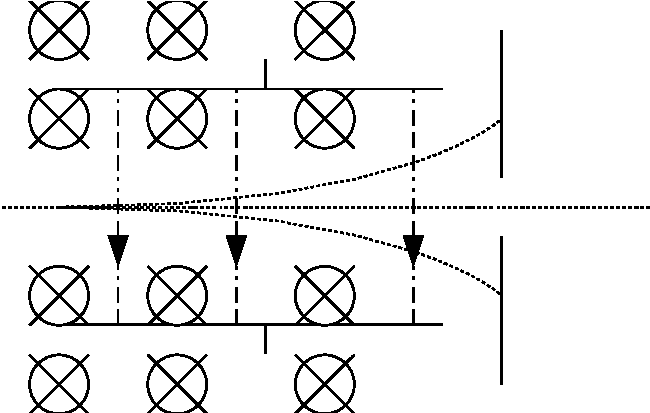
\includegraphics[width=0.42\textwidth]{mat/geschwindigkeitsfilter}
	\caption{Skizze eines Geschwindigkeitsfilters}
	\label{fig:f}
\end{figure}
		
Ein Geschwindigkeitsfilter\index{Geschwindigkeitsfilter} besteht aus einem gekreuzten B-Feld und einem E-Feld. Haben die Teilchen die richtige Geschwindigkeit \(v\), so können sie den Geschwindigkeitsfilter passieren. Der Effekt rührt daher, dass das B-Feld die Teilchen in die andere Richtung ablenkt als das E-Feld. Sind die Teilchen zu schnell, so werden sie vom B-Feld zu stark abgelenkt, sind sie zu langsam, werden sie vom E-Feld zu stark abgelenkt. In Abbildung \ref{fig:f} wirkt die Elektrische Kraft \(F_el\) auf negativ geladene Teilchen nach oben, während die Lorentzkraft \(F_L\) nach unten wirkt. Es gilt dabei:

\begin{equation}
v = \frac{E}{B}
\end{equation}


		\chapter{Elektromagnetische Induktion}

Bei der \textit{Elektromagnetischen Induktion}\index{Elektromagnetischen Induktion} entsteht eine Spannung in einem Leiter, hervorgerufen durch ein Magnetisches Feld. Dies kann auf verschiedene Arten geschehen.

		\section{Relativbewegung}

Bewegt man einen Leiter der Länge \(l\) mit der Geschwindigkeit \(v\) durch ein Magnetfeld der Flussdichte \(B\) (oder das Magnetfeld um den Leiter), so wird in dem Leiter eine Spannung \(U_{ind}\) induziert. Dabei spielt nur die Geschwindigkeitskomponente \(v_s\) senkrecht zu den Feldlinien (und dem Draht) eine Rolle. Für die Richtung des Stromflusses gilt die Linke-Hand-Regel\index{Linke-Hand-Regel}\footnote{Daumen: Bewegungsrichtung des Drahtes, Zeigefinger: Feldlinien, Mittelfinger: Physikalische Stromrichtung}. Es gilt:

\begin{equation}
U_{ind} = v_s \cdot B \cdot l
\end{equation}

		\section{Induktion durch Flächenänderung}
		\label{fland}

Wird eine Leiterschlaufe mit \(n\) Windungen so durch ein homogenes Magnetfeld der Flussdichte \(B\) geführt, dass in der Zeit \(\Delta t\) die vom Feld durchsetzte Schlaufenfläche sich von \(A_1\) auf \(A_2\) ändert\footnote{sich also eine Änderung von \(\Delta A = A_2 - A_1\) ergibt}, so gilt:

\begin{equation}
U_{ind} = n \cdot B \cdot \frac{\Delta A}{\Delta t} = n \cdot B \cdot \dot{A}
\label{eq_fland}
\end{equation}
Durch die Bewegung der Leiterschlaufe am Rande des Magnetfeldes taucht sie also mal mehr und mal weniger ein. Die Flächenänderung kann aber auch als Verformung passieren, oder dass die Leiterschlaufe im Magnetfeld gekippt wird; damit ändert sich nämlich die effektive Fläche, also die Fläche, die zu den Magnetischen Feldlinien senkrecht steht



		\subsection{Sinusspannung}

Somit lässt sich einfach Strom erzeugen, dessen Spannungsverlauf sinusförmig ist. Indem man nämlich eine Spule der Querschnittsfläche \(A_0\) in einem B-Feld rotieren lässt, dass die Rotationsachse senkrecht zu den Feldlinien steht, erhält man eine Fläche \(A_{eff}\) die senkrecht zu den Feldlinien des Magnetfeldes steht, durch die also Induktion stattfinden kann. Es git dabei
\begin{eqnarray}
A_{eff}(t) &=& A_0 \cdot  cos(\varphi) = cos(\omega \cdot t) \\
\dot{A}(t) &=& - A_0 \cdot \omega \cdot sin(\omega \cdot t)
\end{eqnarray}
mit der Kreisfrequenz \(\omega\) und der Zeit der Drehung \(t\), da sich die Spule logischerweise kreisförmig dreht (ihre Seitenkanten beschreiben die Bahn eines Zylinders senkrecht zu den Magentfeldern). Die Flächenänderung \(\dot{A}\) ergibt sich durch die Ableitung nach \(t\). Mittels Formel \ref{eq_fland} kann damit die induzierte Spannung errechnet werden.



		\section{Induktion durch Änderung der Magnetischen Flussdichte}\label{dichland}

In einer Leiterschlaufe mit \(n\) Windungen und der Querschnittsfläche \(A\), die sich senkrecht zu den Feldlinien in einem homogenen Magnetfeld befindet, das in der Zeit \(\Delta t\) von der Flussdichte \(B_1\) auf \(B_2\) geändert wird, ergibt sich:

\begin{equation}
U_{ind} = n \cdot A \cdot \frac{\Delta B}{\Delta t} = n \cdot A \cdot \dot{B}
\label{eq_dichland}
\end{equation}

		\section{Induktionsgesetz}

Kapitel \ref{fland} und \ref{dichland} kann man zu einem einzelnen Gesetz zusammenfassen: Dem \textit{Induktionsgesetz}\index{Induktionsgesetz}. Dafür wird der \textit{Magnetische Fluss} \(\Phi\)\index{Magnetischer Fluss} definiert: Für eine Leiterschlaufe / Spule der Querschnittsfläche \(A\) die sich in einem homogenen Magnetfeld der Flussdichte \(B\) befindet, gilt:

\begin{equation}
\Phi = B \cdot A
\end{equation}
Die Einheit von \(\Phi\) ist \(1 Tm^2 = 1 \frac{N}{A \cdot m} \cdot m^2 = 1 \frac{J}{A} = 1\frac{V \cdot A \cdot s}{A} = 1 V s\)

Möchte man sich \(\Phi\) vernanschaulichen, so kann man sich vorstellen, dass \(\Phi\) die Anzahl der Feldlinien ist, die senkrecht durch die Querschnittsfläche laufen. Die Änderung von einem der beiden Faktoren \(B\) oder \(A\) ruft jeweils eine Induktionsspannung hervor. Kommt in einem Versuch sowohl eine Veränderung von \(A\) als auch von \(B\) vor, so kann man getrennt berechnen, welche Induktionsspannung sich für eine Änderung der durchflossenen Querschnittsfläche ergibt, welche Induktionsspannung sich für die Änderung des B-Feldes ergibt und diese beiden Spannungen addieren, um dann auf die endgültige Induktionsspannung zu kommen. Es gilt also für die Formeln: (\ref{eq_fland}) + (\ref{eq_dichland}) \(\rightarrow\) (\ref{eq_magfl})\footnote{Das hochgestellte Pünktchen bedeutet, dass es sich um eine Ableitung nach der Zeit handelt.}

\begin{equation}
U_{ind} = n \cdot \dot{A} \cdot B + n \cdot A \cdot \dot{B} = n \cdot \dot{\Phi}
\label{eq_magfl}
\end{equation}
Wichtig ist sowohl hier, als auch bei \ref{eq_fland} und \ref{eq_dichland}, dass \(U_{ind}\) zur \emph{Änderung} des Magnetischen Flusses \(\Phi\)
\footnote{also auch zur \emph{Änderung} der senkrecht felddurchsetzten Fläche bzw. der \emph{Änderung} der Flussdichte}
proportional ist. Liegt eine Leiterschlaufe also in einem Magnetfeld, das konstant schwächer wird, so wird eine konstannte Spannung induziert. gleiches gilt, wenn sich die Fläche konstant ändert -- dann wird eine konstannte Spannung induziert.

Zu beachten ist aber auch die Selbstinduktion einer Spule! \(\rightarrow\) Kapitel \ref{selbstind}~!



		\section{Lenz'sche Regel}
		\label{kap_lenzsche_regel}

Die \textit{Lenz'sche Regel}\index{Lenz'sche Regel} besagt, dass ein Induktionsvorgang so verläuft, dass er der Ursache seiner Entstehung entgegenwirkt. 

Wenn also beispielsweise ein Elektromagnet vor einem Metallring eingeschaltet wird, so wird in dem Ring ein solcher Strom induziert, dass das Magnetfeld, welches aus dem Stromfluss im Ring resultiert, entgegen dem der Spule weist.

Die Lenzsche Regel sorgt dafür, dass wir Formel \ref{eq_magfl} abändern müssen:

\begin{equation}
U_{ind} = - n \cdot \dot{\Phi}
\label{eq_lenz}
\end{equation}
Diese neue Induktionsspannung bezieht sich nun auf eine bereits in der Spule bestehende Spannung. Hat man nämlich beispielsweise eine stromdurchflossene Spule und führt in diese Materie ein mit \(\mu_r >> 1\), so sinkt die Stromstärke \(I\) für die Dauer des Einführvorganges. Aus (\ref{eq_langspule}) ist ersichtlich, dass \(B\) steigt. Nach Lenz verläuft die Induktion nun so, dass sie dem Wachstum von \(B\) entgegenwirkt. Ihre Spannung muss also entgegen der "`Urspannung"' sein.

		\section{Selbstinduktion}
		\label{selbstind}

\index{Selbstinduktion}Sobald sich in einer stromdurchflossenen Spule die Stromstärke \(I\) ändert, induziert diese Spule eine Spannung -- eben auch bei sich selbst. Ändert sich nämlich die Stromstärke \(I\) in einer Spule, so sorgt diese Stromänderung für eine Veränderung des Magnetischen Flusses. Aus Kapitel \ref{dichland} folgern wir, dass Induktion stattfinden kann. Diese Induktion findet in der Spule selbst statt, wo eine Spannung induziert wird, die nach der \textit{Lenz'schen Regel} dem Stromfluss, der für die Induktion sorgt, entgegenwirkt. Dabei gilt: \(U_{ind} \sim \dot{I}\). Dieses Phänomen ist als \textit{Selbstinduktion} bekannt. Liegen in einem Stromkreis Schlingungen des Leiters vor, so reagieren diese wie eine Spule.

Die \textit{Induktivität} \(L\) eines Leiters gibt an, wie groß diese entgegengesetzte induzierte Spannung \(U_{ind}\) ist: 
\begin{equation}
U_{ind} = - L \cdot \dot{I}
\label{ind_spule}
\end{equation}
Die Einheit von \(\dot{I}\) ist \(\dot{I} = \frac{A}{s}\)


Die Induktivität\index{Induktivität!allgemein} ist allgemein definiert mit:

\begin{equation}
L = \frac{U_{ind}}{\dot{I}}
\end{equation}
Für \textit{langgestreckte Spulen}\index{Induktivität!langgestreckte Spulen} mit \(n\) Windungen, der Länge \(l\) und mit der Querschnittsfläche \(A\) gilt dabei:

\begin{equation}
L = \mu_0 \cdot \mu_r \cdot n^2 \cdot \frac{A}{l}
\end{equation}
Die Einheit von \(L\) ist : \([L] = \frac{V \cdot s}{A} = \frac{kg \cdot m^2}{C^2} = \frac{kg \cdot m^2}{s^2 \cdot A^2}\)



		\section{Einschaltvorgang eines Spulenstromkreises}
		\label{einschalt}

\index{Einschaltvorgang}Schaltet man einen Stromkreis, in dem eine Spule sitzt, ein, so baut sich die Stromstärke erst mit der Zeit auf. Dies ist ein direktes Resultat der Selbstinduktion. Wenn nämlich der Strom eingeschaltet wird, also in Schaubild \ref{oszi_I} die Funktion sich gerade von der Zeitachse entfernt, ist die Änderung des Stromes \(\dot{I}(t)\) äußerst groß, da sich die Spannung ja von "`überhaupt kein Wert"' auf "`einen positiven Wert"' ändert. Nach Formel \ref{ind_spule} ist die Induktionsspannung hier also stark negativ. Mit dem \textsc{Lenz}'schen Gesetz in Einklang ist diese Induktionsspannung also ihrer Ursache entgegengesetzt und "`\textit{fängt}"' die Veränderung der Stromstärke ab. Der Stromverlauf ist deshalb an dieser Stelle auch kurvenförmig. Ohne die entgegengerichtete Induktionsspannung hätte der Strom sein Maximum praktisch sofort erreicht. So nährt er sich seinem Maximum nur \textit{asymptotisch} an.

Je mehr Zeit innerhalb einer halben Periode verstreicht, desto näher kommt der ausgebremste Strom seinem Maximum, aber immernoch ist eine gegenläufige Spannung da, die ihn dezimiert. Da er konsequent dezimiert wird, wird \(\dot{I}(t_n)\) auch kleiner, da ja ständig die wachstumsschwächende Induktionsspannung auf den Strom einwirkt.

Wenn der Strom dann wieder abgeschaltet wird, also von seinem Maximum abfällt, ist in Schaubild \ref{oszi_U} ein noch größerer Peak\index{Peak} entstanden, der diesmal nach oben zeigt, also auch eine große positive Spannung hinweist. \(\dot{I}(t_n)\) ist an dieser Stelle stark negativ, weil der Strom sich von einem nahezu konstannten Wert "`\textit{erstmalig}"' abbewegt. Nach Gleichung \ref{ind_spule} sorgt diese Spannung nun dafür, dass der Stromstärkenabfall abgefangen wird, also nicht so drastisch aussieht, weshalb sich auch hier wieder ein kurvenförmiger Lauf ergibt.


\begin{figure}[h]
\centering
\subfigure[Stromverlauf]{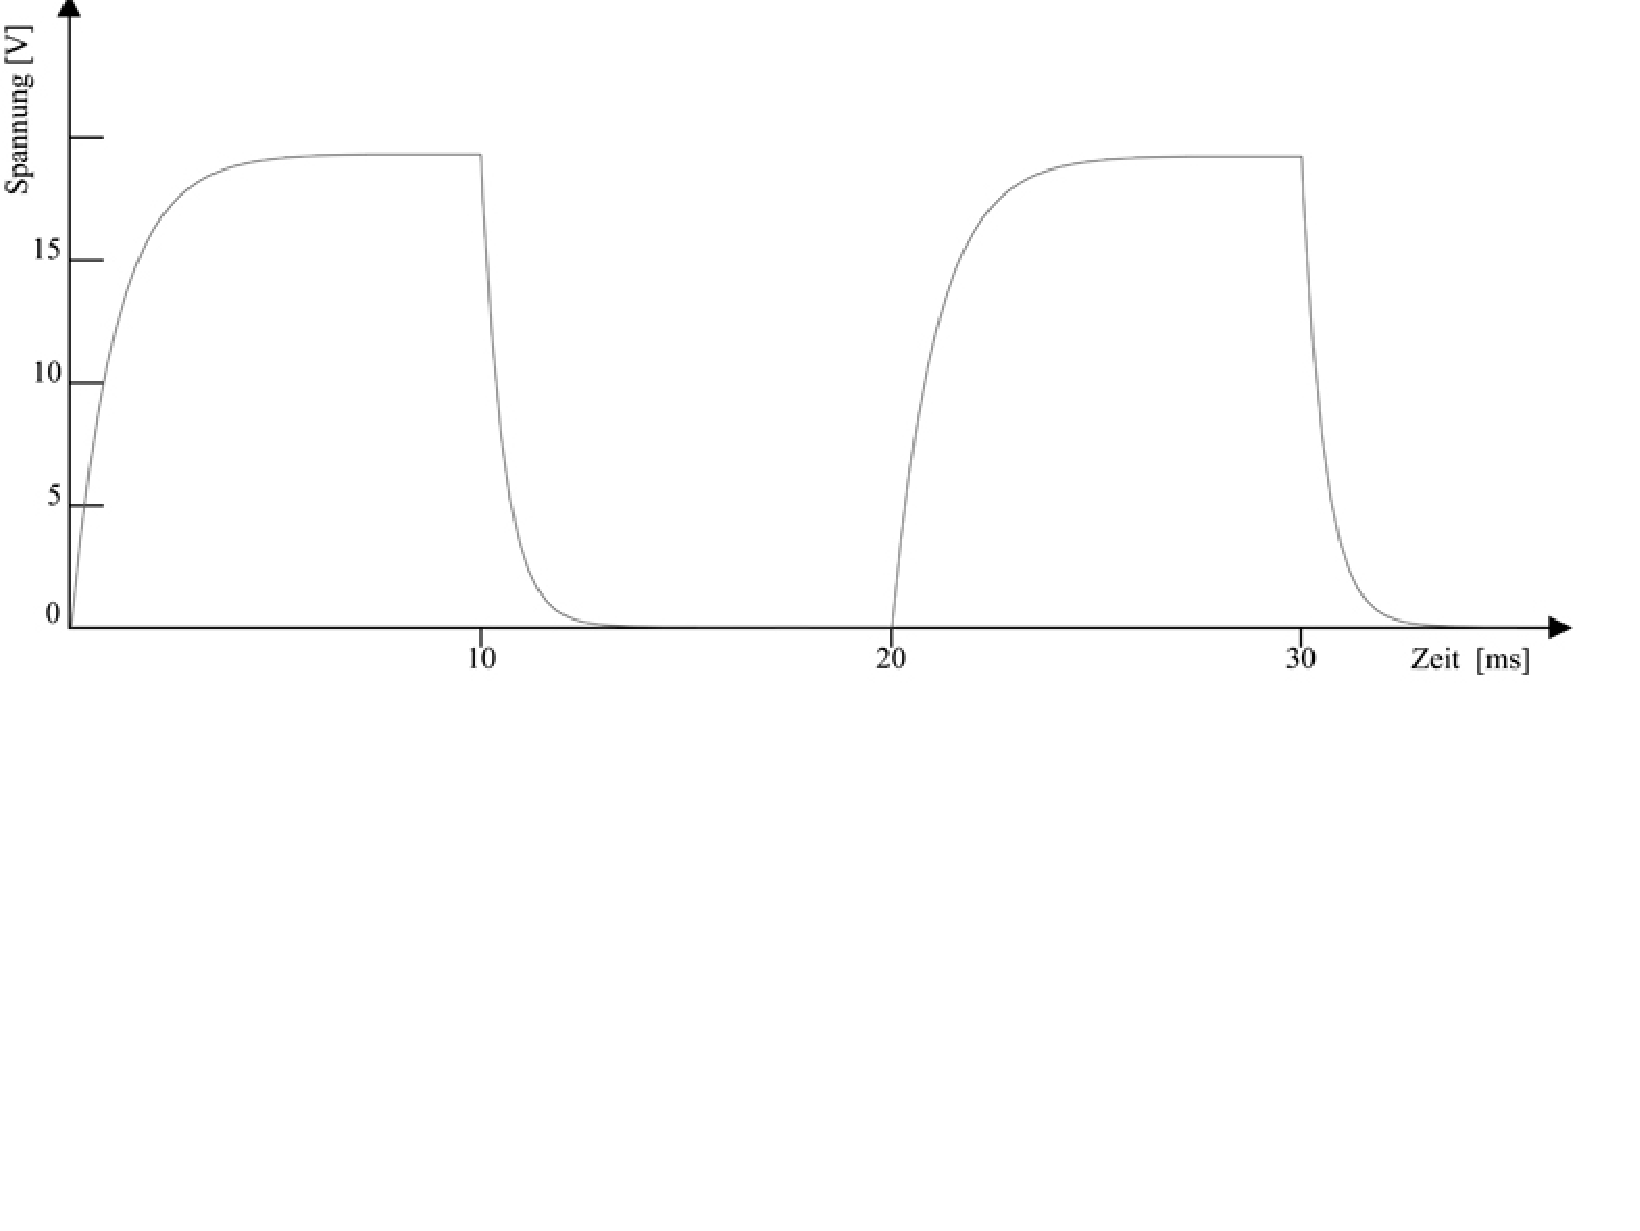
\includegraphics[width=0.45\textwidth]{mat/oszi_I}\label{oszi_I}}
\subfigure[Spannungsverlauf]{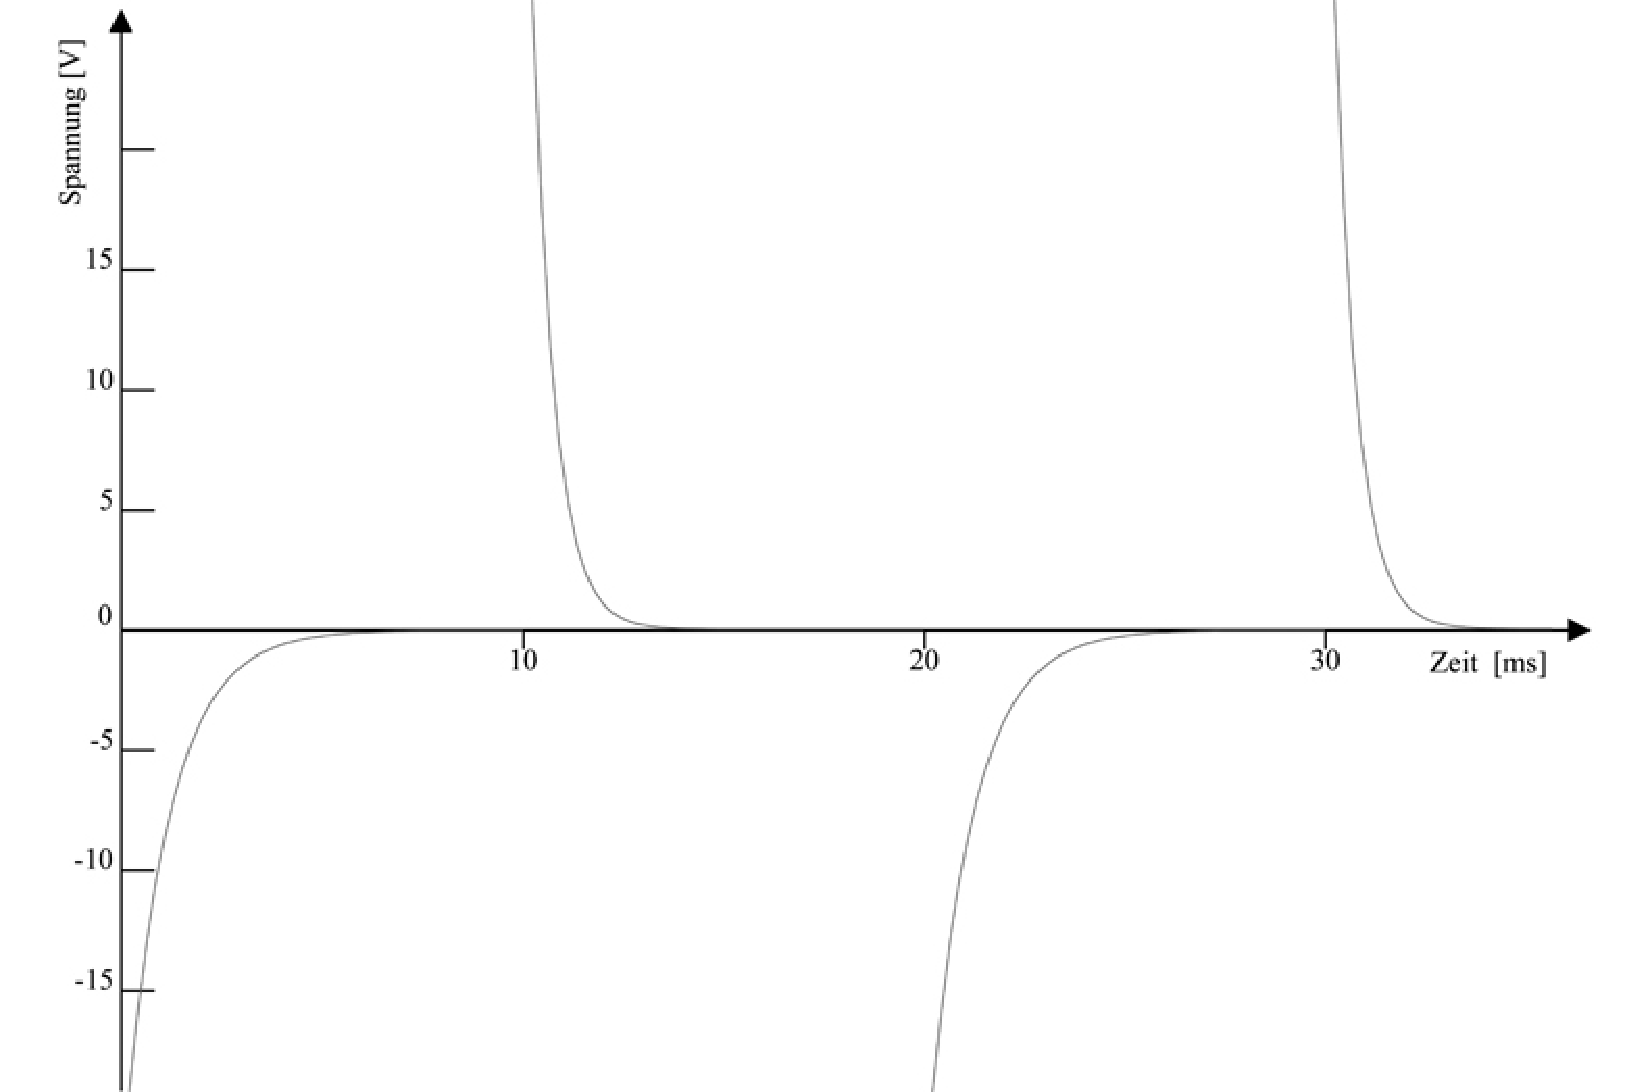
\includegraphics[width=0.45\textwidth]{mat/oszi_U}\label{oszi_U}}
\caption{Vorgänge beim Einschalten eines Stromkreises mit Spule -- siehe Kapitel \ref{einschalt}}
\label{oszi}
\end{figure}



		\section{Energie des Magnetfelds}

Unterbricht man einen Spulenstromkreis, so wird die Spule nach dem \textsc{Lenz}'schen Gesetzt dafür sorgen, dass der Strom noch möglichst aufrecht erhalten wird. Mit diesem Strom kann Arbeit verrichtet werden -- im Magnetfeld muss also Energie gespeichert sein. Die enthaltene Energie des Magnetfeldes zwischen zwei Zeitpunkten \(t_1\) und \(t_2\) berechnet sich mit
\begin{equation}
E_{mag} = \int_{t_1}^{t_2} P(t) dt
\label{int_Emag}
\end{equation}
Mit der Formel für elektrische Leistung \(P_{el} = U \cdot I\) und Formel \ref{ind_spule} ergibt sich so\footnote{Weil \(\dot{I} = \frac{dI}{dt}\) und somit \( \dot{I} \cdot dt = \frac{dI}{dt} \cdot dt = dI\)}
\begin{equation}
E_{mag} = - \int_{t_1}^{t_2} \left ( L \cdot \dot{I}(t) \cdot I(t) \right ) dt = 
- \int_{I(t_1)}^{I(t_2)} \left ( L \cdot I(t) \right ) dI(t) = 
- L \left [ \frac{1}{2} \cdot I^2 \right ]_{I(t_1)}^{I(t_2)}
\label{e_mag}
\end{equation}


% 		\chapter{Definitionen, Größen}
%
% \begin{description}
% 	\item[\(\frac{q}{m}\)] bezeichnet die \textit{Spezifische Ladung} eines Teilchens. Für Elektronen gilt: \( \frac{e}{m}~=~1,7588~\cdot~10^{11}~\frac{C}{kg}\)
% 	\item[\(\mu_r\)] bezeichnet die \textit{Permeabilitätszahl}, die festlegt, um wie viel stärker das Magnetfeld wird, wenn man einen Materiekern einführt.
% \end{description}

%\cleardoublepage
\part{Schwingungen}
		\chapter{Begriffe \& Definitionen}

\begin{description}
	\item[Schwingung] eine sich zeitlich periodisch wiederholende Änderung einer oder mehrerer physikalischer Größen um enen Mittelwert
	\item[Elongation] Auslenkung -- Entfernung von einer Ruhelage zu einem Zeitpunkt \(s(t)\)\index{Elongation}
	\item[Amplitude] Betrag der maximalen Auslenkung \(\hat{s}\)\index{Amplitude}
	\item[Periode(ndauer)] die Dauer einer Vollständigen Schwingung \(T\)
	\item[Frequenz] Anzahl von Schwingungen pro Zeit \(f = \frac{1}{T}\)\index{Frequenz}
	\item[Winkelgeschwindigkeit] Drehung im Bogenmaß je Zeit \(\omega = \dot{\varphi} = 2 \cdot \pi \cdot f\)\index{Winkelgeschwindigkeit}
	\item[Rückstellkraft] Kraft die da Pendel in Richtung der Ruhelage beschleunigt \(F_R\)\index{Rückstellkraft}
	\item[Harmonische Schwingung] eine Schwingung, deren \(t\)-\(s(t)\)-Diagramm sinusförmig ist, wobei \(F_R \sim s(t)\) gilt \index{Harmonische Schwingung}
\end{description}


				\chapter{Harmonische Schwingung}

		\section{allgemeiner Lösungsansatz}

Im Allgemeinen hat sich bei uns der Lösungsansatz etabliert, eine Differentialgleichung zweiten Grades\index{Differentialgleichung} aufzustellen. Dabei wird die Rückstellkraft \(F_R\) auf zwei verschiedene Arten ausgerechnet. Einmal über den Zusammenhang \(F_R = m \cdot a(t)\) und das andere mal über den Zusammenhang \(F_R = - D \cdot s(t)\). Zur Diffenentialgleichung wird die Gleichung dann, weil \(\dot{s}(t) = v(t)\) und \(\dot{v}(t) = a(t)\) und somit \(\ddot{s}(t) = a(t)\). Unser Lösungsansatz ist also im Allgemeinen

	\begin{equation}
	m \cdot \ddot{s}(t) = - D \cdot s(t)
		\label{loesungsansatz}
	\end{equation}
	Die Lösung dieser Gleichung ist dann für uns die \textit{Sinusfunktion}, da
    sie diejenige Funktion ist, die ihrer zweiten Ableitung proportional
    ist\footnote{\(f(x) = \sin(x) ~~ f''(x) = - \sin(x)  ~~ f(x) = - f''(x)\)}. Mit ihr ergibt sich
	\begin{eqnarray}
		s(t) & = & \hat{s} \cdot sin(\omega \cdot t + \varphi) 
			\label{s(t)} \\
		\dot{s}(t) & = & \hat{s} \cdot \omega \cdot cos(\omega \cdot t + \varphi ) \\
		\ddot{s}(t) & = & - \hat{s} \cdot \omega^2 \cdot sin(\omega \cdot t + \varphi)
			\label{a(t)}
	\end{eqnarray}
Mit diesen Gleichungen lässt sich eine harmonische Schwingung beschreiben\footnote{\(\varphi\) ist die Phasenverschiebung}\index{Phasenverschiebung}. Als nachgewiesen, dass es sich bei der Schwingung um eine harmonische Schwingung handelt, gilt es, wenn man zeigen kann, dass
	\begin{eqnarray}
		F_R(t) &=& - D \cdot s(t) 
			\label{F sim s}\\
		D &=& m \cdot \omega^2
	\end{eqnarray}
 für die \emph{komplette} Schwingung gilt.


Setzt man nun Formel \ref{s(t)} und Formel \ref{a(t)} in Formel \ref{loesungsansatz} ein, so ergibt sich\footnote{mit \(\omega = \frac{2 \cdot \pi}{T}\)} für die Periodendauer \(T\) einer periodischen Schwingung allgemein

	\begin{equation}
		T = 2 \cdot \pi \cdot \sqrt{\frac{m}{D}}
			\label{T}
	\end{equation}

		
		
		
		
		\section{Das Fadenpendel}


Bei einem Fadenpendel\index{Fadenpendel} wirkt bei einer Masse immer eine Kraft
\(F_A\) in der Verlängerung des Fadens. Sie ist die Reactio der Zentripetalkraft
\(F_Z\), die den Schwingkörper auf seiner Kreisbahn hält. Zusätzlich greift
jederzeit die Schwerkraft \(F_g\) am Schwingkörper an. Mithilfe eines
Kräfteparallelogramms kann man die Schwerkraft nun zerlegen und erhält
einerseits \(F_A\), andererseits die Rückstellkraft \(F_R\). Diese
weist\footnote{so sie existiert -- im Ruhepunkt nämlich nicht} immer tangential zur Kreisbahn in Richtung der Ruhelage.


	\begin{figure}[h]
		\centering
		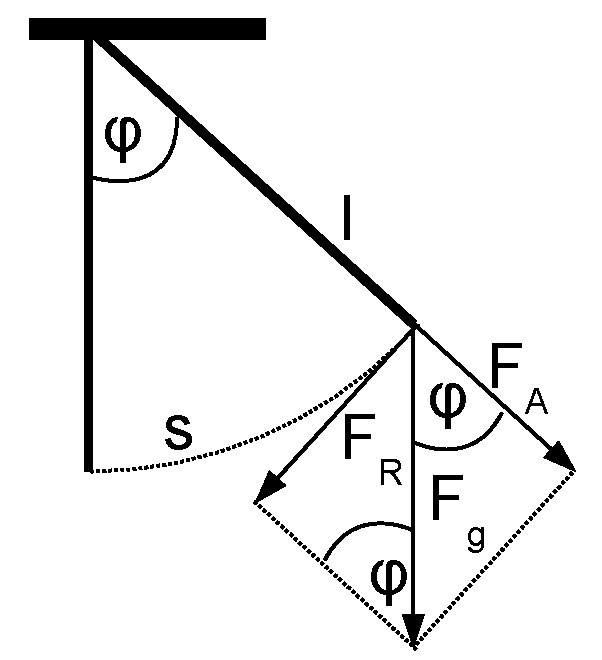
\includegraphics[width=0.35\textwidth]{mat/federpendel}
		\caption{Skizze eines Federpendels mit den bedeutenden Größen eingetragen}
			\label{skizze_federpendel}
	\end{figure}
Vom Nebenwinkelsatz aus kann man den Auslenkungswinkel \(\varphi\) noch an verschiedenen Stellen finden. Hier gelten dann die Beziehungen am rechtwinkligen Dreieck

	\begin{equation}
		\frac{F_R}{F_g} = sin(\varphi) 
			\label{F_R}
	\end{equation}
Der Winkel \(\varphi\) (im Bogenmaß) wiederum ist definiert mit 

	\begin{equation}
		\varphi = \frac{s}{l}
			\label{sinusnaehrung}
	\end{equation}
Für kleine Winkel \(\varphi\) gilt nun \(\varphi \approx sin(\varphi)\). Führt man diese Nährung jetzt entweder bei Formel \ref{F_R} oder bei Formel \ref{sinusnaehrung} durch, so erkennt man, dass

	\begin{equation}
		\frac{F_R}{F_g} \approx \frac{s}{l} ~~ \Rightarrow ~~ F_R \approx \frac{F_g}{l} \cdot s
			\label{naehrungsgleichung}
	\end{equation}
Da sowohl \(F_g = m \cdot g\) als auch \(l\) konstant sind, hängt \(F_R\) bei einer Schwingung nur von \(s\) ab. Damit ist also bewiesen, dass das Fadenpendel für kleine Auslenkungen \(\varphi < 6\)\textsuperscript{o} eine \emph{harmonische Schwingung} ausführt. Seine Richtgröße ist 

	\begin{equation}
		D = \frac{m \cdot g}{l}
			\label{richtgroesse_fadenpendel}
	\end{equation}
		
		
		
		\section{Das Federpendel}
	

Bei einem Federpendel hängt an einer Feder mit der Federhärte \(D\) ein Schwingkörper der Masse \(m\). Die Ruhelage dieses Systems ist dann erreicht, wenn die Kraft, mit der die Feder am Schwingkörper zieht \(F_F\) so groß ist, wie der Schwerkraft \(F_g\). Da bei einer Feder das \textsc{Hook}'sche Gesetz \(D = \frac{F}{s}\) gilt, gilt weiter

	\begin{equation}
		F_F = D \cdot s = - F_g ~~ \Rightarrow ~~ s_0 = - \frac{m \cdot g}{D}
			\label{s_0}
	\end{equation}
\(s_0\) ist dabei die Auslenkung des Pendels vom völlig unausgelenkten Zustand der Feder aus.

Das \textsc{Hook}'sche Gesetz\index{Hook'sches Gesetz} macht hier von Anfang an klar, dass es sich bei der Schwingung um eine harmonische handelt. Die Federhärte entspricht der Richtgröße\footnote{beide heißen deshalb \(D\)}. Besteht ein System aus einem Schwingkörper zwischen zwei Federn, so gilt für die Richtgröße
\begin{equation}
	D = D_1 + D_2
\end{equation}
		
	
	
		\section{Das Wasserpendel}

Ein Wasserpendel\index{Wasserpendel} besteht aus einem U-Rohr mit dem konstanten Querschnitt \(A\) in das Wasser der Masse \(m_{ges}\) mit der Dichte \(\varrho\) gefüllt wird. Die Wasseroberflächen in den beiden Rohrteilen stehen einander gegenüber und die Wassersäule hat insgesamt die Höhe \(2 \cdot h_0\), weil \(h_0\) die (gebogene) Strecke vom unteren Rohrmittelpunkt bis zu einem der Wasserspiegel ist. Die Schwingung mit der Elongation \(s(t)\) schwingt um diesen Pegelstand\footnote{\(h(t) = h_0 + s(t)\)}.


Wird nun das Wasser auf Seite A um \(s^{+}\) ausgelenkt, so sinkt der Pegel auf Seite B um \(- s^{+}\). Die Wassersäule ist auf Seite A \(2 \cdot s^{+}\) höher. Dieses \textit{Mehr} an Wasser \(V^{+}\) erfährt nun die Gewichtskraft \(F_g = m^{+} \cdot g\) nach unten, die gleichzeitig als Rüchstellkraft \(F_R\) fungiert. Über die Zusammenhänge von Masse, Dichte und Volumen (\(m = \varrho \cdot V\)) und der Umrechnung des Volumens (\(V^{+} = A \cdot 2 \cdot s^{+}\)) ergibt sich so für die Rückstellkraft
	
	\begin{equation}
		F_R = g \cdot \varrho \cdot A \cdot 2 \cdot s^{+}
			\label{rueckstellkraft_wsserpendel}
	\end{equation}
Dabei sind außer \(s^{+}\) alles Konstanten. Es ergibt sich für das Wasserpendel also eine Richtgröße \(D\) \index{Richtgröße} von

	\begin{equation}
		D = 2 \cdot g \cdot \varrho \cdot A
			\label{richtgroesse_wasserpendel}
	\end{equation}




		\section{Der Schwingkreis}


Ein Schwingkreis\index{Schwingkreis} ist ein Stromkreis, der im einfachsten Falle lediglich einen Kondensator\index{Kondensator} der Kapazität \(C\) und eine Spule\index{Spule} der Induktivität\index{Induktivität} \(L\) enthält. In ihm schwingt Strom der Ladung \(Q\) zwischen Kondensator und Spule hin und her. Aufgrund des simplen Aufbaus\footnote{Die Spannung des Kondensators \(U_C\) liegt direkt an der Spule an, ebenso wie die Induktionsspannung \(U_{ind}\) direkt am Kondensator anliegt} gilt im Stromkreis

	\begin{eqnarray}
		U_{ind} &=& - L \cdot \dot{I}(t) = - L \cdot \ddot{Q}(t)
			\label{U_spule} \\
		U_C &=& \frac{Q(t)}{C} = \frac{1}{C} \cdot Q(t)
			\label{U_kondensator} \\
		U_C &=& U_{ind} 
			\label{U = U}
	\end{eqnarray}
Der Kondensator wird anfangs einmalig geladen. Somit steckt im Kondensator
Energie \(E_{el}\). Der Kondensator entlädt sich nun langsam über die Spule,
dabei fließt logischerweise Strom -- und zwar mehr Strom, als zu dem Zeitpunkt
da der Kondensator noch ungeladen war -- somit steigt \(\dot{I}(t)\). Es ergibt
sich nach den Gleichungen \ref{U_spule} und \ref{U = U} eine
Induktionsspannung.\index{Induktionsspannung}\index{Lenz'sche Regel} Diese wirkt
dem Stromfluss entgegen (Siehe Kap. \ref{kap_lenzsche_regel} auf S.
\pageref{kap_lenzsche_regel}) und damit kann sich der Kondensator nicht sofort
entladen. Der Entladestrom nähert sich nun langsam (asymptotisch) seinem Maximum
an. 

In der Zeit, in der der Kondensator entladen wurde, baute sich in der Spule (und rundherum) ein Magnetfeld auf. Dieses Magnetfeld speichert nun die Energie \(E_{mag}\), die der Kondensator vorher enthalten hatte (\(E_{el} = E_{mag}\)). Wenn der Kondensator schließlich leer ist, ergibt sich erneut eine Induktionsspannung. Da der Strom vorher einen relativ großen Wert hatte und nun völlig "`abgeschaltet"' ist, wird \(\dot{I}(t)\) infolgedessen stark negativ und es wird erneut Spannung induziert, die den bereits abgebrochenen Stromfluss weiter unterhält.

Durch diese Induktionsspannung wird der Kondensator nun wieder geladen. Wenn das Magnetfeld komplett abgebaut ist, wird der Kondensator wieder so viel Energie haben, wie direkt nach dem Aufladen\footnote{von Verlusten der Dämpfung sei hier abgesehen}. Die Platte, die vorher aber negativ war, ist jetzt positiv und anderstherum. Das E-Feld hat sich also umgekehrt. Wenn der Vorgang dann wieder von Vorne beginnt, wird auch das B-Feld der Spule in die andere Richtung weisen als zuvor.

Es handelt sich hierbei um eine harmonische Schwingung, bei der Stromstärke und Spannug einer Sinusfunktion folgen. Setzt man die Gleichungen \ref{U_spule} und \ref{U_kondensator} in Gleichung \ref{U = U} ein, so erhält man eine Differentialgleichung \(\ddot{Q}(t) = - \frac{1}{L \cdot C} \cdot Q(t)\) deren Lösung wieder eine Sinusfunktion ist:\index{Differenzialgleichung}
	\begin{eqnarray}
		Q(t) &=& \hat{Q} \cdot cos(\omega \cdot t)
			\label{schwingkreis_Q} \\
		I(t) &=& - \hat{I} \cdot sin(\omega \cdot t)  = - \frac{\hat{Q}}{\sqrt{L \cdot C}} \cdot sin(\omega \cdot t) \\
		U(t) &=& \hat{U} \cdot cos(\omega \cdot t)
	\end{eqnarray}
Für den Schwingkreis ergibt sich eine Periodendauer von
	\begin{equation}
		T = 2 \cdot \pi \cdot \sqrt{L \cdot C}
	\end{equation}
Will man mechanische und elektrische Schwingungen Vergleichen, so gelte folgende Entsprechungen:
	\begin{eqnarray*}
	s 	& \widehat{=} & Q \\
	v 	& \widehat{=} & I \\
	a & \widehat{=} & \dot{I} \\
	D & \widehat{=} & \frac{1}{C} \\
	m & \widehat{=} & L \\
	\frac{1}{2} \cdot D \cdot s^2 & \widehat{=} & \frac{1}{2} \cdot  \frac{1}{C} \cdot  Q^2 \\
	\frac{1}{2}  \cdot m  \cdot v^2 	& \widehat{=} & \frac{1}{2}  \cdot L  \cdot I^2 
	\end{eqnarray*}


				\chapter{Gedämpfte Schwingungen}

\index{Gedämpfte Schwingung}Im Gegensatz zur idealen harmonischen Schwingung nimmt die Amplitude\index{Amplitude} \(\hat{s}\) im Laufe der Schwingung ab. Energie der Schwingung wird in andere Energieformen umgewandelt. Dies geschieht im Allgemeinen durch Kräfte \(F_{gl}\) die aus der Reibung schwingender Systeme resultieren. 

	\section{Konstante Reibung} 
Konstante Reibung tritt bspw. bei mechanischen Schwingungn auf. Hierbei ist die Bremsende Kraft \(F_{gl}\) konstant. Es gilt also für die Rückstellkraft \(F_R\)
	\begin{equation}
		F_R = m \cdot \ddot{s}(t) = - D \cdot s(t) - F_{gl}
	\end{equation}
Es gilt also hier das lineare Kraftgesetz nicht mehr und somit handelt es sich nicht um eine harmonische Schwingung. Die Amplitude \(\hat{s}\) der Schwingung nimmt bei jeder Schwingung \textit{linear} um \(s^{-}\) ab, mit
	\begin{equation}
		s^{-} = \frac{2 \cdot F_{gl}}{D}
	\end{equation}
	
	
	\section{Reibung abhängig von der Geschwindigkeit} 
Geschwindigkeitsabhängige Reibung tritt beispielsweise bei der Wirbelstrombremse\index{Wirbelstrombremse} auf. Hierbei nimmt die Amplitude \(\hat{s}\) zwischen den einzelnen Schwingungen exponentiell ab. Für die Rückstellungskraft ergibt sich hierbei
	\begin{equation}
		F_R = m \cdot \ddot{s}(t) = - D \cdot s(t) - R \cdot \dot{s}(t)
	\end{equation}
\(R\) ist hierbei eine Reibungskonstante. Auch hier liegt keine harmonische Schwingung vor. Eine Lösung der Differentialgleichung\footnote{\(m \cdot \ddot{s}(t) = - D \cdot s(t) - R \cdot \dot{s}(t)\)} ist hierbei die Funktion
	\begin{equation}
		s(t) = \hat{s} \cdot e^{- k \cdot t} \cdot sin(\omega \cdot t)
	\end{equation}
wobei \(\omega\) von der Eigenfrequenz\footnote{also der Frequenz, die das System ohne Reibung ausführen würde}  \(\omega_0\) abweicht. Hier gilt
	\begin{equation}
		\omega = \sqrt{\omega_0^2 - k^2}
	\end{equation}
Wobei auch \(k\) eine Reibungskonstante ist mit \(k = \frac{R}{2 \cdot m}\).

Bei dieser Art der Schwingungen muss man zwischen drei verschiedenen Sorten unterscheiden:
	
\begin{description}
	\item[Schwingfall]\index{Schwingfall} \(\omega_0 > k^2\) Das System Schwingt und die Amplitude nimmt exponentiell ab
	\item[Aperiodischer Grenzfall]\index{Aperiodischer Grenzfall} \(\omega_0 = k^2\) Das System schwingt fast eine halbe Periode lange, die Amplitude geht jedoch in kürzestmöglicher Zeit gegen null.
	\item[Kriechfall]\index{Kriechfall} \(\omega_0 < k^2\) Das System schwingt nur kurz in eine Richtung, dann nimmt die Amplitude relativ langsam ab.
\end{description}
	Es kann auch sein, dass Der Zusammenhang zwischen Reibung und Geschwindigkeit komplexer ist oder sich im Laufe einer Periode verändert.....




		\chapter{Erzwungene Schwingung}

Das Gegenteil einer gedämpften Schwingung ist eine erzwungene Schwingung.\index{Erzwungene Schwingung} Dabei wird von Außen auf das schwingende System Einfluss ausgeübt. Dieser Einfluss erfolgt periodisch, jedoch nicht notwendigerweise mit der Eigenfrequenz \(\omega_0\) der Schwingung sondern auch mit anderen Frequenzen \(\omega\). Zur Rückstellkraft \(F_R\) kommt also noch eine weitere Kraft \(F_1\) hinzu mit 
	\begin{equation}
		F_1(t) = \hat{F}_1 \cdot sin(\omega \cdot t + \varphi)
	\end{equation}
Für eine gedämpfte Schwingung ergibt sich also
	\begin{equation}
		F_R(t) = m \cdot \ddot{s}(t) = - D \cdot s(t) - k \cdot \dot{s}(t) + F_1(t)
	\end{equation}
\(~\)\\
Je nachdem, wie sich \(\omega\) und \(\omega_0\) zueinander verhalten, unterscheidet man zwischen drei verschiedenen Fällen:
	
	\begin{itemize}
	\item \(\omega \rightarrow 0\): Das System passt sich der Schwingung des Zwanges an und schwingt ohne Phasenverschiebung.
	\item \(\omega = \omega_0\): Es kommt zur \emph{Resonanz}.\index{Resonanz} Das System schwingt um \(\varphi = \frac{\pi}{2} = 90\)\textsuperscript{o} \emph{hinter} dem Zwang. Hierbei wächst seine Amplitude stark an.
	\item \(\omega \rightarrow \infty\): Die Amplitude sinkt sehr stark und das System schwingt mit einer Phasenverschiebung von \(\varphi = \pi = 180\)\textsuperscript{o} hinter dem Zwang her.
	\end{itemize}

%\cleardoublepage
\part{Wellen}

		\chapter{Definition Mechanische Welle}

Eine Mechanische Welle\index{Welle!mechanische}\index{Mechanische Welle} tritt dann auf, wenn ein \emph{Wellenträger}\footnote{Es kann sich dabei um feste, flüssige oder gasförmige Materie handeln}\index{Wellenträger} eine \emph{Störung}\index{Störung} weiterleitet, ohne dass dabei die Teilchen des Wellenträgers wandern - sie bewegen sich nur am Ort. Dabei wird Energie\footnote{kinetische und potentielle Energie} transportiert. Die Geschwindigkeit, mit der sich die einzelnen Teilchen des Wellenträgers bewegen, wird als \emph{Schnelle} \(\vec{v}\)\index{Schnelle} bezeichnet.

Eine Welle breitet sich dabei mit einer bestimmten \emph{Ausbreitungsgeschwindigkeit} \(c\)\index{Ausbreitungsgeschwindigkeit} aus. Diese ist vom Wellenträger abhängig.\footnote{Es kann auch dazu kommen, dass die Ausbreitungsgeschwindigkeit von der Frequenz der Schwingung abhängt; das bezeichnet man als \emph{Dispersion}\index{Dispersion}.} Es kann dabei sein, dass sich nur eine einzelne Störung ausbreitet, es kann sich aber auch um einen periodischen Vorgang handeln.

\index{Longitudialwellen}\index{Transversalwellen}\index{Querwellen}\index{Längswellen}Man unterscheidet dabei zwischen Longitudinal- oder Längswellen und Transversal- bzw. Querwellen. Bei \emph{Longitudinal}wellen bewegen sich die Teilchen des Wellenträgers \emph{in} Ausbreitungsrichtung, bei \emph{Transversal}wellen bewegen sie sich senkrecht zur Ausbreitungsrichtung.



		\chapter{Feder-Massen-Modell}

Das Feder-Massen-Modell\index{Feder-Massen-Modell} dient dazu, sich die Ausbreitung einer Störung vorstellen zu können: In diesen Modell liegen Massenteilchen in einer Reihe und werden von Federn miteinander verbunden. Wird nun eines dieser Teilchen angeregt - bspw. nach oben gezogen -, so spricht man hier von einer Störung - schließlich wurde die geradlinige Anordnung der Teilchen gestört. Durch die Feder dieses ersten Massenteilchens zu seinem Nachbarn - durch die Störung wurde sie gespannt - wird dieser nun nach oben gezogen, wodurch er die nächste Feder spannt, die nun wiederum den nächsten Massenpunkt nach oben zieht. Durch die Trägheit der Massen der einzelnen Teilchen vergeht ein gewisser Zeitraum, bis ein Massenteilchen so weit ausgelenkt ist, wie sein Nachbar\footnote{daraus resultiert die Ausbreitungsgeschwindigkeit}. Auf diese Weise breitet sich die anfängliche Störung durch den kompletten Wellenträger aus - sieht man von Reibung u.ä. ab.




		\chapter{Harmonische Wellen}

Eine \emph{Fortschreitende Welle}\index{Fortschreitende Welle} ist das, was man sich für gewöhnlich unter dem Begriff ``Welle'' vorstellt. Dabei wird dem Wellenträger periodisch Energie zugeführt und die Massenteilchen bewegen sich mit gleichartigen, erzwungenen Schwingungen. Handelt es sich bei diesen Schwingungen der einzelnen Massenteilchen um harmonische Schwingungen, so wird die Welle als \emph{Harmonische Welle}\index{Harmonische Welle} bezeichnet.

Ein bestimmter Schwingungszustand\footnote{Das entspricht einem Bestimmten Winkel \(\varphi\) im Zeigerformalismus\index{Zeigerformalismus} (Kap. \ref{sss_zeigerdarstellung}).} breitet sich dabei mit der Geschwindigkeit \(c\) aus. Betrachtet man also zwei Teilchen, die genau \(c \cdot t_1\) auseinanderliegen, und phasengleich schwingen\footnote{also jederzeit mit dem selben Winkel \(\varphi\) darstellbar sind}, so muss es sich bei \(t_1\) um ein Vielfaches von der \emph{Schwingungsdauer} \(T\) handeln. \(T\) ist der kürzeste zeitliche Abstand zwischen zwei Teilchen, die phasengleich schwingen. Die kürzeste Distanz zwischen zwei Teilchen, die Phasengleich schwingen, wird als \emph{Wellenlänge} \(\lambda\) bezeichnet. Es gilt als Zusammenhang

\begin{equation}
 	c = \frac{\lambda}{T} = \lambda \cdot f
 	\label{eq_cLf}
\end{equation}


			\section{Wellengleichung}

\index{Wellengleichung!Mechanische Welle}Nun lässt sich einfach eine Wellengleichung herleiten, die dazu dient, die Auslenkung eines beliebigen Teilchens einer Welle zu einer beliebigen Zeit zu bestimmen. Dazu nimmt man an, dass die Welle sich linear ausbreitet und zwar in positive \(x\)-Richtung. Bei \(x =0\) wird die Welle periodisch angeregt, zum Zeitpunkt \(t = 0\) wird sie das erste mal in positive \(s\)-Richtung ausgelenkt.

Am Punkt \(x = 0\) schwingt das Teilchen also mit einer harmonischen Schwingung. Seine Amplitude ist \(\hat{s}\) und seine Drehfrequenz ist \(\omega\), dadurch beträgt sein Drehwinkel \(\varphi\) zum Zeitpunkt \(t\):  \(\varphi = \omega \cdot t\).  Die Gleichung zu seiner Schwingung lautet somit:
\begin{equation}
 	s(t) = \hat{s} \cdot sin(\omega \cdot t)
		\label{eq_s(t,x0)}
\end{equation}
Dieses Teilchen regt nun seine Nachbarn in positiver \(x\)-Richtung an und überträgt seine Bewegung darauf. Da sich diese Ausbreitung mit der Geschwindigkeit \(c\) vollzieht, hat jedes Teilchen, das vom ersten weiter als
\begin{equation}
 	x(t) = c \cdot t \Rightarrow t(x) = \frac{x}{c}
		\label{eq_x(t)}
\end{equation}
entfernt ist, keine Auslenkung - die erste Störung ist noch nicht bis zu ihm durchgedrungen.

Betrachtet man nun ein Teilchen, das nach Formel \ref{eq_x(t)} schon schwingen muss, so kann man auf dessen Auslenkung ganz einfach schließen, indem man berechnet, wie lange die Welle sich vom ersten Teilchen bis hierher ausgebreitet hat. Diese Dauer ergibt sich mit Formel \ref{eq_x(t)}. Aus der bereits verstrichenen Zeit \(t\) und dieser Zeit ergibt sich die Zeit, zu der das Teilchen an der Stelle \(x = 0\) den gesuchten Schwingungszustand hatte. Somit setzt man diese Zeit in Formel \ref{eq_s(t,x0)} ein, und erhält die gesuchte Auslenkung:
\begin{equation}
	s(x,t) = \hat{s} \cdot sin\left(\omega \cdot \left(t - \frac{x}{c}\right)\right) = \hat{s} \cdot sin\left(\frac{2 \cdot \pi}{T} \cdot \left(t - \frac{x}{\frac{\lambda}{T}}\right)\right) = \hat{s} \cdot sin\left(2 \cdot \pi \cdot \left(\frac{t}{T} - \frac{x}{\lambda}\right)\right)
		\label{eq_s(x,t)}
\end{equation}
Die Umformung erhält man mit \(\omega = \frac{2 \cdot \pi}{T}\) und \(c = \frac{\lambda}{T}\).

Diese Formel beschreibt nun für eine Schwingung die Auslenkung für beliebige Zeitpunkte und an beliebigen Orten. Sie kann auf drei verschiedene Arten verwendet werden:
\begin{enumerate}
 \item Auslenkung eines einzelnen Punktes zu einer Bestimmten Zeit:\\
	Dazu muss man in die Formel schlicht Abstand \(x\) vom ersten angeregten Teilchen und die Zeit \(t\) seit dem Beginn von dessen Anregung.

\item Ein Momentanbild der Schwingung erzeugen:\\
	Hierzu gibt man schlicht die Zeit seit Beginn der Anregung des ersten Teilchens in die Formel ein und wird eine \(s(x)\)-Gleichung erhalten. Dabei muss man aber beachten, dass diese Gleichung zum Schaubild einer Sinus-Welle gehört, die in beide Richtungen ins Unendliche geht. Die Welle ist zu einem Bestimmten Zeitpunkt aber noch nicht so weit fortgeschritten. Ab einem bestimmten Punkt (mit Formel \ref{eq_x(t)} zu berechnen), sind die Teilchen noch nicht ausgelenkt.

\item Die Schwingung eines speziellen Teilchens in der Zeit erzeugen:\\
	Hierbei geht man entsprechend vor - man setzt den \(x\)-Wert des Teilchens ein und beachtet dabei, dass vor \(t = 0\) keine Schwingung stattgefunden haben kann, sondern erst ab der durch Formel \ref{eq_x(t)} zu bestimmenden Zeit.
\end{enumerate}




\subsubsection{Phasenverschiebung}

\index{Phasenverschiebung}Bei den Berechnungen für eine Wellengleichung sind wir stets davon ausgegangen, dass das Teilchen bei \(x = 0\) zum Zeitpunkt \(t = 0\) angeregt wird und vorher noch nicht ausgelenkt war. Ist dies nicht der Fall, so muss man dies als \emph{Phasenverschiebung}\footnote{Im Prinzip die Phasendifferenz zum idealen Zustand.} berücksichtigen. Sie drückt sich in einem Winkel \(\varphi_0\) aus, der als konstanter Wert stets zum Drehwinkel \(\omega \cdot t\) addiert wird:
\begin{equation}
 	\varphi(t) = \omega \cdot t + \varphi_0
\end{equation}
Hat ein Massenteilchen an \(x = 0\) bei \(t = 0\) bereits die Auslenkung \(s_1\), so beträgt die Phasenverschiebung 
\begin{equation}
 	\varphi_0 = sin^{-1}\left (\frac{s_1}{\hat{s}} \right )
\end{equation}








			\section{Zeigerdarstellung}
			\label{sss_zeigerdarstellung}

\index{Zeigerformalismus!Definition}Dadurch, dass die einzelnen Massenteilchen der Harmonischen Welle harmonische Schwingungen ausführen, lassen sie sich auch leicht mit dem Zeiger-Formalismus darstellen. Jedem einzelnen Teilchen wird ein gedachter, im Kreis rotierender Zeiger zugeordnet, dessen Länge der Maximalen Auslenkung des Teilchens entspricht. Die Rotationsfrequenz des Zeigers entspricht der Frequenz des schwingenden Teilchens. Der Anteil des Zeigers, parallel zur Schnelle, entspricht der Auslenkung des einzelnen Teilchens.






		\chapter{Reflexion}
		
		
				\section{Festes Ende}


\index{Reflexion}\index{Festes Ende}Bei einer Reflexion an einem festen Ende drehen sich sowohl Schnelle \(v\), als auch Ausbreitungsrichtung \(c\) um. Dabei zieht das letzte - befestigte - Wellenträgerteilchen seine letzten Vorgänger zurück in die Ausgangslage, nachdem sie von der Schnelle bewegt wurden. Dieses \textit{Zurückgezogen-Werdens} des Wellenträgers wird damit zur neuen Schnelle.
				
				\section{Loses Ende}

\index{Loses Ende}Bei Reflexion am losen Ende dagegen, behält die Schnelle \(v\) ihre Richtung bei, während nur die Ausbreitungsgeschwindigkeit \(c\) ihre Richtung umkehrt. Hierbei können sich die letzten Wellenträger frei bewegen. Sie werden von der Schnelle bewegt, und ziehen ihre Vorgänger dann mit in die selbe Richtung; dieses \textit{Mitgezogen-Werden} wird hierbei zur neuen Schnelle.


				\section{Konstruktionshilfe}
				
Zur Konstruktion einer durch Reflektion resultierenden Welle gibt es kleine Tricks. Dazu stellt man sich die Welle einfach weiter hinter dem reflektierenden Ende vor. Der \textit{'überschüssige'} Wellenteil wird dann
\begin{description}
 \item[Festes Ende] am festen Punkt punktgespiegelt.
 \item[Loses Ende] an der Achse, auf der sich das lose Ende bewegt, gespiegelt.
 \end{description}
Diese Spiegelungen addiert man dann schlicht zu der hinlaufenden Welle und hat als Resultierende Welle die Reflexion.

Um diese reflektierten Wellen mathematisch auszudrücken kann man analog zu Formel \ref{eq_s(x,t)} auf S. \pageref{eq_s(x,t)} die folgenden Formeln verwenden. Für Reflektion am \emph{festen Ende} gilt:
\begin{equation}
 	s_r(x,t) = - \hat{s} \cdot sin\left(2 \cdot \pi \cdot \left(\frac{t}{T} - \frac{(2 \cdot L - x)}{\lambda}\right)\right)
\end{equation}
Und für Reflektion am \emph{losen Ende} gilt:
\begin{equation}
 	s_r(x,t) = \hat{s} \cdot sin\left(2 \cdot \pi \cdot \left(\frac{t}{T} - \frac{(2 \cdot L - x)}{\lambda}\right)\right)
\end{equation}
Bei der Reflektion gibt es jedoch zu bedenken, dass die reflektierte Welle nach der Zeit \(t_1\) erst eine bestimmte Strecke \(x_1\) zurückgelegt hat, so dass sie erst \emph{ab} dem folgenden Punkt schwingt:
\begin{equation}
 	x_1 = 2 \cdot L - c \cdot t_!
\end{equation}




				\section{Im Zeigerformalismus}

\index{Zeigerformalismus!Reflexion}Im Zeigerformalismus sieht eine Reflexion beim festen und losen Ende unterschiedlich aus. Beim \emph{festen Ende} erfolgt ein so genannter \textit{Phasensprung}. Das bedeutet, dass an dem Teilchen, an dem reflektiert wird, der Zeiger der herlaufenden Welle genau in die Gegenrichtung zeigt, wie der Zeiger der reflektierten Welle. Das ist logisch, da die Summe der beiden Vektoren an dieser Stelle einen Nullvektor ergeben muss.

Bei Reflektion am \emph{losen Ende} dagegen, tritt der Phasensprung nicht auf. Hier kann das letzte Teilchen sich frei bewegen. Die Zeiger für hinlaufende und reflektierte Welle sind an dieser Stelle identisch - deshalb ergibt sich hier auch eine doppelt so hohe Amplitude.






		\chapter{Überlagerung}
		
\index{Ueberlagerung von Wellen@Überlagerung von Wellen}\index{Interferenz}Treffen zwei Störungen oder Wellen auf einem Wellenträger aufeinander, so durchdringen sie sich ungestört. Dabei addieren sich jedoch die Elongationen und Schnellen der beiden Wellen - es sieht aus, als hätte man eine neue Welle. Diesen Vorgang bezeichnet man als \emph{Interferenz}


		\section{Eindimensionaler Wellenträger}

\subsubsection{Gleichlaufende Wellen}
\label{par_Gleichlaufende Wellen}

Laufen zwei Wellen in die gleiche Richtung und haben darüber hinaus noch die selbe Wellenlänge \(\lambda\), so unterscheiden sie sich voneinander durch den \emph{Gangunterschied}\index{Gangunterschied} \(\delta\) bzw. die Phasendifferenz \(\Delta \varphi\)\index{Phasendifferenz}. Der Gangunterschied ist die räumliche Distanz zwischen zweimal den selben Schwingungszuständen auf den verschiedenen Wellen, die Phasendifferenz gibt dagegen an, wie sich die Phasen der beiden Wellen in \emph{einem} Punkt unterscheiden. Diese beiden Größen ändern sich für die beiden Wellen nicht. Es gilt der Zusammenhang
\begin{equation}
 	\frac{\Delta \varphi}{2 \cdot \pi} = \frac{\delta}{\lambda}
 	\label{eq_zshg_phasendif_ganguntersch}
\end{equation}
Im Allgemeinen entsteht so aus harmonischen Wellen einer Frequenz eine neue harmonische Welle der selben Frequenz.

Es kann nun zu \emph{Sonderfällen} kommen: Wenn der Gangunterschied nahe an oder genau auf der Wellenlänge liegt (\(\delta \approx \lambda\)) - und somit die Phasendifferenz gegen \(0\) strebt \(\Delta \varphi \rightarrow 0\) - kommt es zur \emph{konstruktiven Interferenz}\index{Konstruktive Interferenz}\index{Interferenz!Konstruktive}. Hierbei liegen nämlich Wellenberge und -täler stets aufeinander und ergeben somit eine Maximale Amplitude:
\begin{equation}
 	\delta = k \cdot \lambda ~~~ k = (0; 1; 2; 3; \ldots)
 		\label{eq_bedingungen_konstruktiveinterferenz}
\end{equation}
Im Entgegengesetzten Fall dagegen kann es zur \emph{destruktiven Interferenz} kommen\index{Destruktive Interferenz}\index{Interferenz!Destruktive}, wenn der Gangunterschied die Hälfte der Wellenlänge ausmacht \(\delta \approx \frac{\lambda}{2}\) und somit die Phasendifferenz an jedem Punkt \(\Delta \varphi \approx \pi\), liegen die Wellenbäuche der einen Welle den Wellentälern der zweiten Welle gegenüber. Durch die Addition entstehen hier minimale Amplituden:\footnote{Ist \(\hat{s_1} = \hat{s_2}\), so ist keine Welle mehr erkennbar, weil die Wellenbäuche und Täler einander aufheben.}
\begin{equation}
 	\delta = k \cdot \lambda - \frac{\lambda}{2} ~~~ k = (1; 2; 3; \ldots)
 		\label{eq_bedingungen_destruktiveinterferenz}
\end{equation}


\subsubsection{Gegenläufige Wellen}

Laufen zwei Wellen aufeinander zu, so durchdringen sie sich ebenfalls und addieren ihre Amplituden und Schnellen. Hierbei ergibt sich ebenfalls ein Spezialfall: Die \emph{Stehende Welle}. Sie kommt jedoch nur unter bestimmten Bedingungen zustande, nämlich wenn beide Wellen die selbe Amplitude \emph{und} die selbe Wellenlänge haben.



		\section{Kreis- und Kugelwellen auf mehrdimensionalen Wellenträgern}

\index{Kreiswellen}\index{Kugelwellen}Bei mehrdimensionalen Wellenträgern - also bspw. Wellen in Wasser (2D) oder Schallwellen in Luft (3D) - kann es zu komplexeren Interferenzmustern kommen. Neben sich linear ausbreitenden \emph{Ebenenwellen}, deren \emph{Wellenfront}\index{Wellenfront}\footnote{Diejenigen Bereiche, in denen die Teilchen im selben Schwingungszustand sind. Zwei Wellenfronten haben somit den Abstand \(\lambda\). Sie liegen immer senkrecht zu der bzw. den Ausbreitungsrichtung(en). (Eine Kreiswelle hat viele radiale Ausbreitungsrichtungen.).} eine gerade Linie bildet, kommen nämlich auch Wellen vor, deren Wellenfronten rund sind. Eine Ebenenwelle kann man sich auch als "`langgezogene"' zweidimensionale Welle vorstellen.
 
Die Prinzipien bei der Interferenz sind dabei jedoch die selben: Die Wellen durchdringen sich gegenseitig und addieren dabei ihre Amplituden. Bei einer Kreis- oder Kugelwelle kommt es so aber zu besonderen Mustern. Es ist dabei nötig, dass die Wellen \emph{kohärent} sind, damit sie interferieren können - d.h. dass zwischen ihnen eine feste, zeitlich unveränderliche Phase(nbeziehung) (\(\Delta\varphi = const\)) besteht.

Bei Kreiswellen bilden sich hyperbelförmige \emph{Knotenlinien}. Hier löschen die Wellen sich die ganze Zeit über aus (destruktive Interferenz). Diese Linien entsprechen den Knotenpunkten bei linearen Wellen. Entsprechend liegen auch Stellen, an denen die Schwingungen besonders stark sind (konstruktive Interferenz) auf hyperbelförmigen Linien. Je weiter der Abstand zwischen den Wellenursprüngen ist, desto mehr Interferenzlinien ergeben sich, ebenso entstehen mehr Interferenzlinien, wenn die Frequenz der Wellen erhöht wird. 

Nach dem Verfahren in \ref{par_Gleichlaufende Wellen} (S. \pageref{par_Gleichlaufende Wellen}) kann man bestimmen, ob man an bestimmten Punkten konstruktive oder Destruktive Interferenz hat. Der Gangunterschied an einem Punkt ergibt sich aus der Differenz der Entfernungen von den beiden Wellenursprüngen
\begin{equation}
 \delta = s_1 - s_2
\end{equation}
Wobei \(s_1\) die Entfernung des Punktes vom ersten und \(s_2\) die Entfernung des Punktes vom zweiten Ursprung ist.

%Um zu ermitteln, ob sich an einem Punkt konstruktive oder destruktive Interferenz ergibt, testet man den \emph{Gangunterschied}, den die Wellen an diesem Punkt haben




		\chapter{Stehende Welle}

\index{Stehende Welle}Bei der stehenden Welle sieht man die Bewegung in eine der Ausbreitungsrichtungen nicht mehr. An bestimmten Punkten - den \emph{Knotenstellen}\index{Schwingungsknoten}\index{Knotenstellen} - bewegen sich die Teilchen des Wellenträgers nicht. Diese Stellen haben den Abstand von \(\frac{\lambda}{2}\) voneinander. Die Abschnitte dazwischen - sog. \emph{Schwingungsbäuche}\index{Schwingungsbäuche} - schwingen ``auf der Stelle''. Also schwingen in diesem \(\frac{\lambda}{2}\) langen Bereich alle Teilchen des Wellenträger phasengleich, wobei die Amplituden der Teilchen sich folgendermaßen berechnen lassen:
\begin{equation}
 	\hat{s}_r(x') = 2 \cdot \hat{s}_1 \cdot sin \left ( \frac{\pi}{2} + \frac{\Delta \varphi}{2} \right ) \cdot sin(2 \cdot \pi \frac{x'}{\lambda}) = 2 \cdot \hat{s}_1 \cdot sin \left ( \frac{\pi}{2} + \frac{\pi \cdot \delta}{\lambda} \right ) \cdot sin(2 \cdot \pi \frac{x'}{\lambda})
\end{equation}
dabei ist \(\hat{s}_r\) die Amplitude eines Teilchens, das \(x'\) von einem Knotenpunkte entfernt ist und \(\hat{s_1}\) ist die (gleichen) Amplituden der Einzelnen Wellen.

Stehende Wellen ergeben sich häufig aus Reflexionen. Dabei läuft der eigentlichen Welle ihre Reflektion entgegen - mit der gleichen Wellenlänge und der gleichen Amplitude\footnote{Bei perfekter Reflexion ohne Reibungsverluste zumindest.}. (Beachte \ref{sss_randbedingungen} auf S. \pageref{sss_randbedingungen})





			\section{Stehende Welle im Zeiger-Formalismus}

\index{Zeiger-Formalismus!Stehende Welle}Eine Welle auf einem Wellenträger besteht im Prinzip aus Masseteilchen, von denen jedes einzelne eine harmonische Schwingung ausführt. Ein benachbartes Teilchen führt ebenfalls diese harmonische Schwingung aus, jedoch schwingt es leicht phasenverschoben. Benutzt man das Zeiger-Modell für die Schwingungen der einzelnen Massenteilchen, so hat man eine Gerade (bildlich die \emph{Ruhelage}), auf der im Abstand der Massenteilchen Vektorpfeile angebracht sind, die alle die selbe Länge haben und ich die selbe Richtung rotieren mit der selben Drehfrequenz.\footnote{Die Komponente des Vektorpfeils senkrecht zu der Geraden repräsentiert die Auslenkung des einzelnen Massenteilchens} Im Abstand von \(\lambda\) sind zwei Vektorpfeile somit gleichphasig. Die Ausbreitung der Welle geschieht nach diesem Modell so, dass ein Massenteilchen durch die Anregung seines Nachbarn auch einen "`\textit{baugleichen}"' Vektorpfeil übertragen bekommt.

Treffen nun zwei Wellen der gleichen Wellenlänge\footnote{Die einzelnen Vektorpfeile drehen mit auch der selben Geschwindigkeit} gegenläufig aufeinander, so hat vor dem Treffen jedes Massenteilchen seinen Vektorpfeil. Beim Treffen bekommt dann das erste Massenteilchen zwei Vektorpfeile - von jedem seiner Nachbarn einen, und ausgehend von diesem ersten Teilchen bekommen auch die Teilchen seiner Umgebung mit der Ausbreitung der beiden Wellen einen zweiten Vektorpfeil.

Jedes Teilchen verfügt nun also über zwei Vektorpfeile, die mit der selben Drehfrequenz rotieren. Dadurch besteht ein fester Winkel zwischen den beiden Vektorpfeilen, der sich nicht ändert. Die Auslenkung des Massenteilchens wird nunmehr durch die Vektorsumme der beiden Vektorpfeile bestimmt\footnote{bzw. deren Komponente senkrecht zur Ruhelage}. Es entsteht so also aus den Vektorsummen eine neue Schwingung. Da der Winkel der Vektorpfeile der Teilschwingungen sich nicht ändert, kommt es an bestimmten Stellen dazu, dass hier die Phasendifferenz zwischen den Vektorpfeilen \(\Delta\varphi = \pi + 2 \cdot n \cdot \pi\) ist, und somit der Summenvektor ein Nullvektor \(\vec{0}\) ist. An dieser Stelle schwingt die neu entstandene Welle somit nie; man nennt sie \textit{Schwingungsknoten}. An anderen Stellen ist die Phasenverschiebung \(\Delta\varphi = 0 + 2 \cdot n \cdot \pi\), somit ist der Additionsvektor hier stets maximal lang. An dieser Stelle kann die Schwingung ihre maximale Auslenkung erreichen; diese Stelle nennt man \textit{Schwingungsbauch}.




			\section{Randbedingungen}
			\label{sss_randbedingungen}

\index{Randbedingungen}Wenn auf einem beschränkten Wellenträger eine stehende Welle durch Reflexion entstehen soll, so müssen bestimmte Randbedingungen erfüllt werden. Die Welle muss an einem Ende reflektiert werden. In einer ersten Phase wird sich so auf jeden Fall\footnote{Ohne Reibung} eine Stehende Welle bilden - eben weil praktisch eine identische Welle zurückläuft. Sobald die stehende Welle jedoch die Seite erreicht hat, auf der sie angeregt wird, muss das anregende Teilchen in einem bestimmten Schwingungszustand sein. 

Um wieder den Zeiger-Formalismus heranzuziehen: Wenn sich bei der stehenden Welle durch Addition zweier Einzelwellen-Vektoren ein Vektor am Punkt der Anregung ergeben hat, so muss dieser der selbe sein, wie das anregende\footnote{bzw. angeregte} Teilchen von sich aus\footnote{bzw. von der Anregung aus} hätte bzw. hat.

Aus diesem Grund ist eine stehende Welle nur auf beschränkten Wellenträgern mit bestimmten Längen \(L\) möglich. Allgemein kann man die Frequenzen, bei denen sich die stehenden Wellen ausbilden berechnen mit 
\begin{equation}
 f = \frac{c}{\lambda}
\end{equation}

Allgemein ist es bei einem Wellenträger gegebener Länge möglich, mehrere verschiedene stehende Wellen darauf hervorzurufen (charakterisiert durch verschiedene \(k\)). Diese verschiedenen Schwingungen haben bestimmte Namen.


Man unterscheidet zwischen verschiedenen Umständen:


\subsubsection{Zwei lose Enden}

Für zwei lose Enden gilt der Zusammenhang
\begin{equation}
 	L = k \cdot \frac{\lambda}{2} \Rightarrow f_k = \frac{2 \cdot k \cdot c}{4 \cdot L} ~~~~ k = (1;2;3;...)
 	\label{eq_2lose}
\end{equation}
\(k\) gibt in diesem Falle die Anzahl an Schwingungsknoten an. Der Wellenträger muss also mindestens halb so lang sein, wie die stehende Welle. 


\subsubsection{Zwei feste Enden}

Bei zwei festen Enden ergibt sich der selbe Zusammenhang wie bei zwei losen Enden, nur dass der Faktor \(k\) hierbei die Anzahl der Schwingungsbäuche angibt.


\subsubsection{Ein festes und ein loses Ende}

Hierbei gilt der Zusammenhang
\begin{equation}
 	L = k \cdot \frac{\lambda_k}{4} ~~~~ k = (1;3;5;...)
 	\label{eq_lose_fest}
\end{equation}
Für \(k\) dürfen hier nur ungerade Werte gewählt werden, weil die Welle in diesem Fall am einen Ende des Wellenträgers einen Bauch und am anderen Ende einen Knoten haben muss. Somit kommt für jeden erlaubten \(k\)-Schritt eine halbe Wellenlänge hinzu. Man könnte die Formel deshalb auch umformulieren zu
\begin{equation}
 	L = k \cdot \frac{\lambda}{2} - \frac{\lambda}{4} \Rightarrow f_k = \frac{(2\cdot k - 1) \cdot c}{4 \cdot L} ~~~~ k = (1;2;3;...)
\end{equation}
Diese Darstellung hätte den Vorteil, dass \(k\) wie bei der anderen Formel gewählt wird und dass man eindeutig sagen kann, dass \(k\) die Anzahl der Wellenbäuche\footnote{am losen Ende ist nur ein \emph{halber} Wellenbauch, er wird trotzdem mitgezählt} ist.


\subsubsection{Nomenklatur der Wellen}


Allgemein ist es bei einem Wellenträger gegebener Länge möglich, mehrere verschiedene stehende Wellen darauf hervorzurufen (charakterisiert durch verschiedene \(k\)). Diese verschiedenen Schwingungen haben bestimmte Namen.

\index{Nomenklatur von Wellen}\index{Harmonische}\index{Grungschwingung}\index{Oberschwingung}Allgemein wird die Schwingung mit der niedrigsten Frequenz - und somit der größt möglichen Wellenlänge - auf einem Wellenträger unter den gegebenen Umständen als \emph{Grundschwingung} oder \emph{1. Harmonische} bezeichnet. Die nächst mögliche, höherfrequente Schwingung wird als \emph{Oberschwingung} oder \emph{2. Harmonische} bezeichnet, dann wird schlicht bei jeder folgenden Schwingung die Ordnungszahl der Harmonischen erhöht.

Bei den Formeln \ref{eq_2lose} und \ref{eq_lose_fest} kann man davon sprechen, dass der Faktor \(k\) für die \(k\). Harmonische steht.





		 \chapter{Beugung}

\index{Beugung}Bei der Beugung weicht Licht an einem Hindernis vom geradlinigen Strahlengang ab. Zu erklären ist das mit dem \textsc{Huygen}'schen Prinzip (\(\rightarrow\) \ref{ss_huygensches prinzip}): Bspw. wird an einem Spalt, auf den die Wellenfront einer Ebenenwelle trifft, nur eine Elementarwelle durchgelassen, die sich dann Kreisförmig \emph{hinter} dem Spalt in alle Richtungen ausbreiten kann und somit auch Bereiche erfasst, die keine geradlinige, offene Verbindung zum Wellenursprung haben.

	\section{Das \textsc{Huygen}'sche Prinzip}
	\label{ss_huygensches prinzip}

\index{Huygen'sches Prinzip}Das \textsc{Huygen}'sche Prinzip dient dazu, Vorgänge rund um "`Wellen"' zu erklären. Dabei wird angenommen, dass eine Welle aus vielen kreisförmigen\footnote{in der 3. Dimension kugelförmigen} \emph{Elementarwellen}\index{Elementarwellen} besteht, die sich überlagern. So bilden die Wellenfronten vieler Elementarwellen durch Überlagerung die Wellenfront einer Welle. Von der Front dieser Wellen gehen wiederum Elementarwellen aus, die sich in einer neuen Wellenfront überlagern (\(\rightarrow\) Fortschreiten der Welle). Kommt eine Welle bspw. an einem Spalt an, so geht an diesem Spalt eine der Elementarwellen als Kreisförmige Welle weiter, während die anderen Elementarwellen zurückgeworfen werden.






	\section{Beugung am Doppelspalt}
	\label{ss_beugung_doppelspalt}

\index{Beugung!Am Doppelspalt}\index{Interferenz}Hierbei kann man sich vorstellen, dass durch jeden einzelnen Spalt nur eine Elementarwelle hindurchtritt. Es ergibt sich so ein Interferenzmuster dieser beiden Elementarwellen, das so aussieht, als würden zwei Kreiswellen dort erzeugt, wo der Spalt liegt. Das Maximum, welches direkt der Mitte zwischen den beiden Spalten gegenüberliegt\footnote{vorausgesetzt dass das einfallende Licht senkrecht zur Doppelspaltebene einfällt} bezeichnet man als \emph{Maximum 0. Ordnung}, anschließend wird ausgehend davon hochgezählt. Bei den Minima benennt man das erste neben dem Maximum 0. Ordnung als \emph{Minimum 1. Ordnung}.\index{Nomenklatur von Wellen}

In Abbildung \ref{img_beugungamdoppelspalt} auf Seite \pageref{img_beugungamdoppelspalt} ist ein Versuchsaufbau dargestellt, mit dem man bspw. die Wellenlänge von Licht bestimmen kann. Grundvoraussetzungen sind dabei, dass Kohärenzbedingungen für das Licht erfüllt sind und dass paralleles Licht senkrecht zur Doppelspaltebene einfällt.

Bei der Beugung am Doppelspalt ergibt sich rein theoretisch für die Verteilung der Intensitäten ein Interferenzbild wie in Abbildung \ref{img_intensitaet_doppelspalt} auf Seite \pageref{img_intensitaet_doppelspalt}. Rein praktisch nimmt die Intensität jedoch ab, je weiter man vom Maximum 0. Ordnung entfernt ist. Das kommt daher, dass sich hier zwei Interferenzphänomene überlagern: Einmal die Interferenz am Doppelspalt und dann noch die Interferenz am Einfachspalt (Siehe Kap. \ref{kap_interferenz_einzelspalt}). Die Interferenzbilder zweier Einfachspalte überlagern sich nämlich zusätzlich und stecken damit die maximal erreichbare Intensität unter den jeweiligen Winkeln ab. Weil die beiden Spalte so nahe aneinander liegen, fallen die Interferenzbilder der beiden Einzelspalte jedoch praktisch aufeinander.



\begin{figure}
   \centering
   
   
   
   \subfigure[Intensitätsverteilung bei der Beugung am Doppelspalt -- theoretisch! Die Phasendifferenz \(\Delta \varphi\) kann dabei in Distanzen \(d_k\) auf dem Schirm umgerechnet werden: \(d_k = tan \left (asin \left (\frac{\frac{\Delta \varphi}{2 \cdot \pi} \cdot \lambda}{g} \right ) \right ) \cdot a \)]{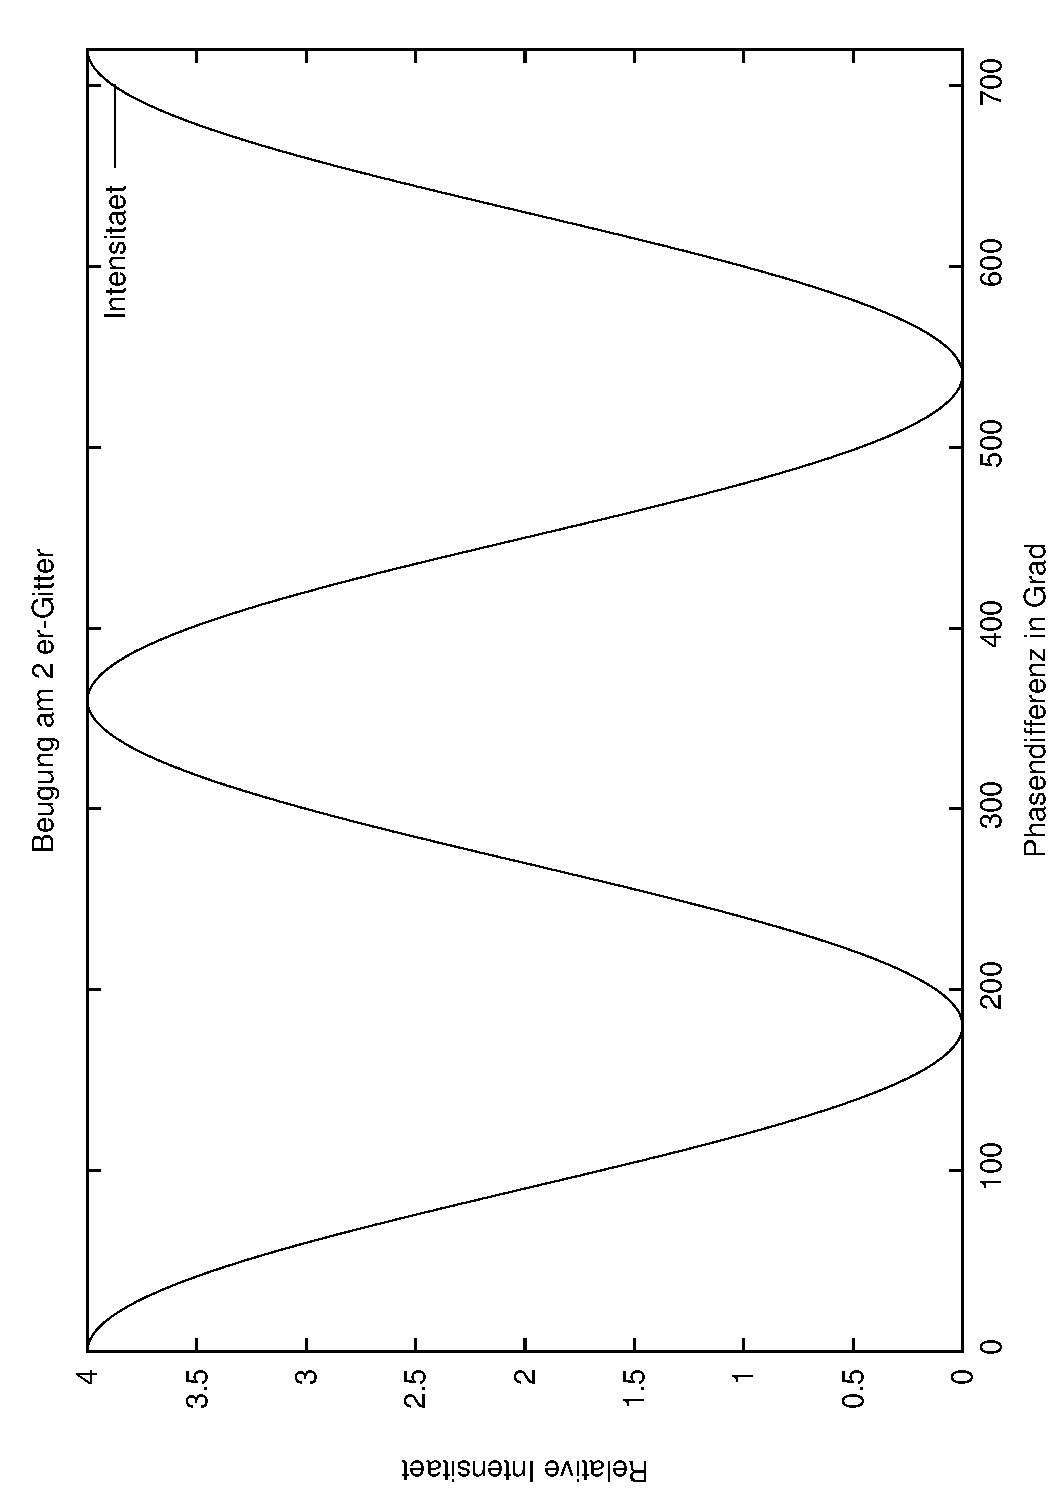
\includegraphics[width=0.43\textwidth,angle=-90]{mat/Intensitaet_doppelspalt}\label{img_intensitaet_doppelspalt}}
   
   \subfigure[Intensitätsverteilung bei Beugung am Einzelspalt (Spaltbreite 3000 nm, Wellenlänge 440 nm)]{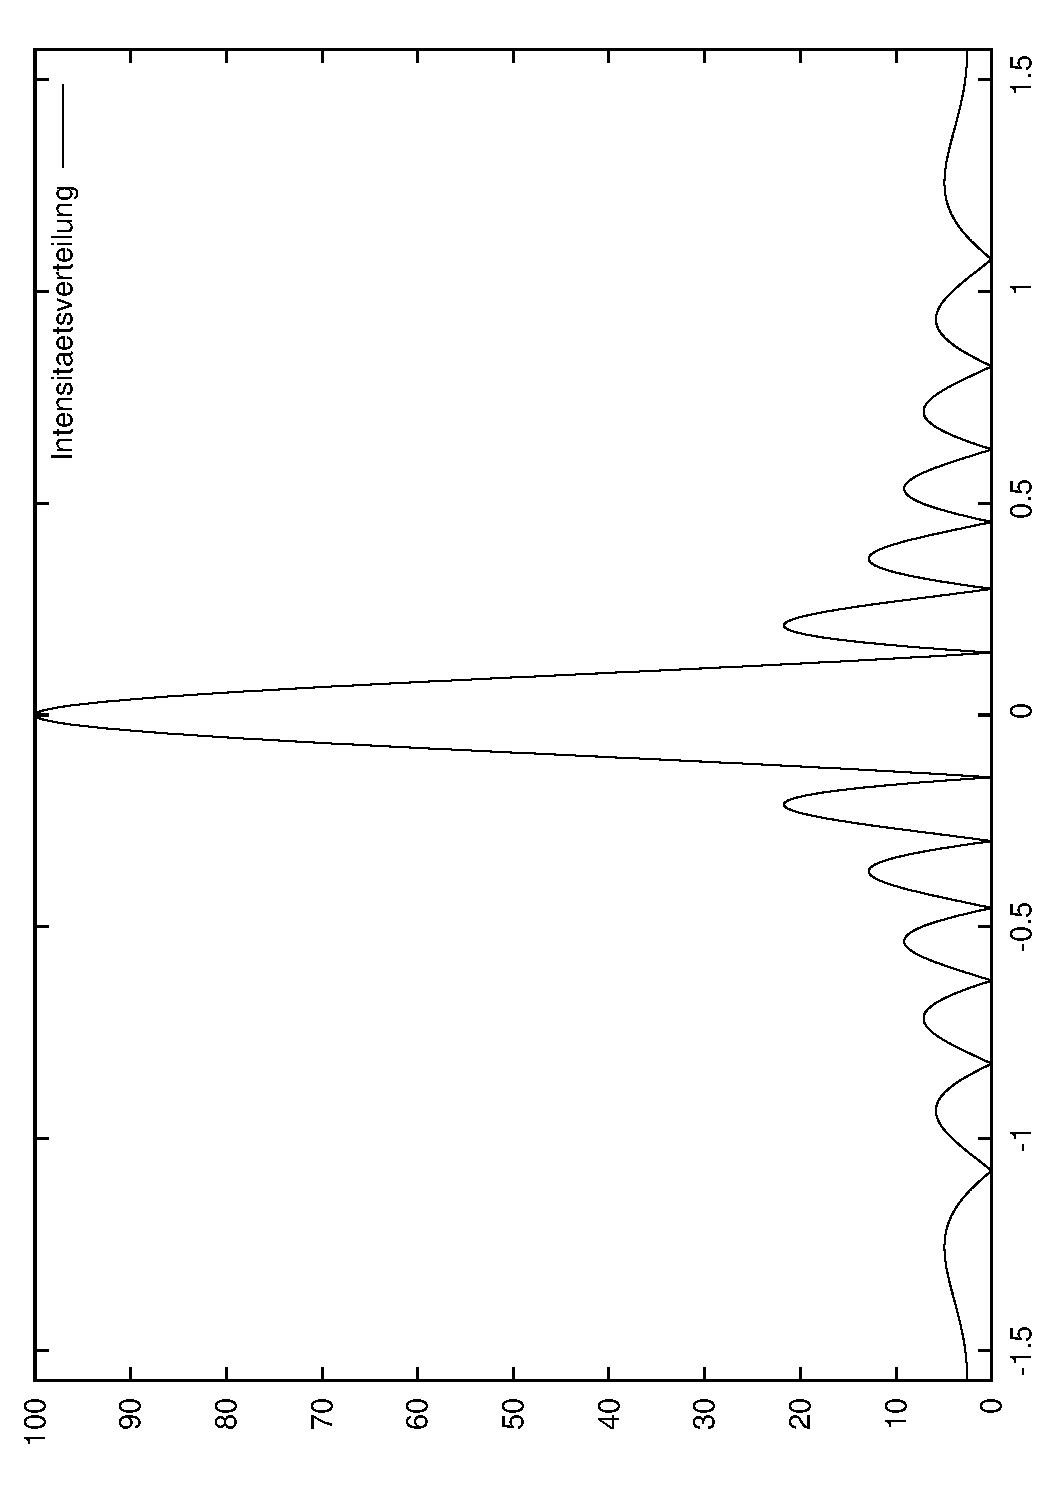
\includegraphics[width=0.43\textwidth,angle=-90]{mat/intensitaet_einzelspalt}\label{img_intensitaet_einzelspalt}}
   
   \subfigure[Intensitätsverteilung bei Beugung am Gitter bei 10 Spalten -- theoretisch!]{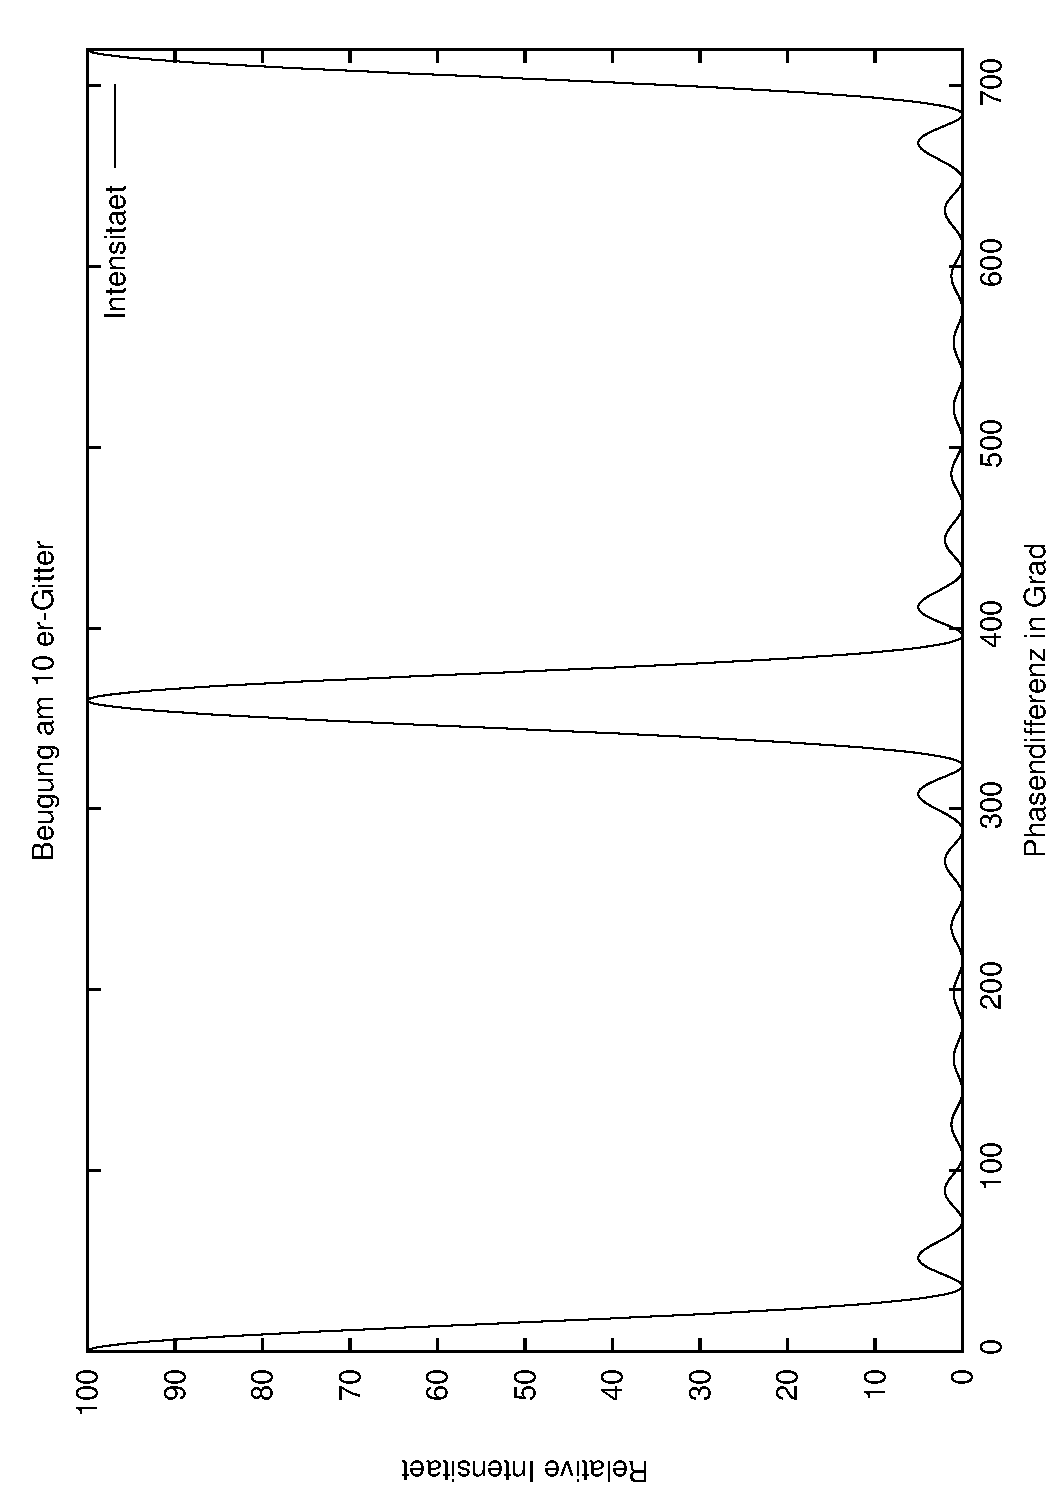
\includegraphics[width=0.43\textwidth,angle=-90]{mat/Intensitaet_zehnerspalt}\label{img_intensitaet_zehnerspalt}}
   
  
   \caption{Diverse Intensitätsverteilungen}
     
\end{figure}



		\section{\textsc{Fraunhofer}-Näherung} 
\index{Fraunhofer-Näherung!Erste}Gilt außerdem bei der Beugung am Doppelspalt
\begin{equation}
a \gg g\\
 	\label{eq_aggg}
 \end{equation}
 \begin{equation}
a \gg d_k
 	\label{eq_aggdk}
\end{equation}
so kann man sich einigen Rechenaufwand sparen. Durch Formel \ref{eq_aggg} ist nämlich der Winkel \(\alpha_k\) nicht nur unter der Linie vom Punkt zwischen den Spalten zum Punkt auf den Leuchtschirm und der Horizontalen zu finden sondern auch näherungsweise zwischen den beiden Lichtstrahlen und einer gedachten Waagerechten. Außerdem sind die beiden Lichtstrahlen dadurch praktisch parallel und (nur) deswegen kann man den Winkel \(\alpha_k\) direkt an den Spalten wiederfinden (S. Skizze). Dadurch ergibt sich ein ähnliches Dreieck\footnote{Der Winkel \(\alpha_k\) und ein rechter Winkel findet sich sowohl in den kleinen Dreieck am Doppelspalt (in der Skizze teilweise. fein gestrichelt und fett) als auch in dem Dreieck, mit dem \(\alpha_k\) bestimmt wird (in der Skizze gestrichelt).} und so kann man hier auch den Gangunterschied \(\delta\) wiederfinden (in der Skizze fett). Dadurch ergibt sich
\begin{equation}
 	\delta = g \cdot sin(\alpha_k)
 		\label{eq_gangunterschied_doppelspalt}
\end{equation}
Je nachdem, ob man einen hellen oder einen dunklen Punkt in Z betrachtet, nimmt man eine der beiden Bedingungen aus Formel \ref{eq_bedingungen_konstruktiveinterferenz} (heller Punkt) oder \ref{eq_bedingungen_destruktiveinterferenz} (dunkler Punkt) an.\footnote{Der Wert für \(k\) entspricht dabei der \emph{Ordnung} des Minimums bzw. Maximums.} 

\index{Fraunhofer-Näherung!Zweite}Bei geraden Schirmen kann man nun noch weiter vereinfachen. Der Abstand \(d_k\) ist über den geometrischen Zusammenhang
\begin{equation}
 	\frac{d_k}{a} = tan(\alpha_k) \Rightarrow d_k = a \cdot tan(\alpha_k)
 		\label{eq_doppelspalttangens}
\end{equation}
gegeben. Für \emph{sehr kleine} Winkel \(\alpha_k\) gilt
\begin{equation}
 	sin(\alpha_k) \approx \alpha_k \approx tan(\alpha_k)
 		\label{eq_winkelnaehrung}
\end{equation}
Und diese kleinen Winkel werden erreicht, wenn Formel \ref{eq_aggdk} gilt. Tut sie das \emph{nicht}, so ist diese zweite Vereinfachung nicht zulässig. Bei der Untersuchung von Lichtwellen ist dies aber normalerweise der Fall und so kann man Formel \ref{eq_gangunterschied_doppelspalt}, Formel \ref{eq_doppelspalttangens} und Formel \ref{eq_winkelnaehrung} mit den Bedingungen aus Formel \ref{eq_bedingungen_konstruktiveinterferenz} bzw. \ref{eq_bedingungen_destruktiveinterferenz} kombinieren:

Für einen maximal hellen Punkt Z bzw. ein Maximum \(k\). Ordnung gilt näherungsweise
\begin{equation}
 \delta = g \cdot \frac{d_k}{a} = k \cdot \lambda ~~~ k = (0; 1; 2; 3; \ldots)
 \label{eq_fraunhoferII_max}
\end{equation}
und dementsprechend gilt für einen dunklen Punkt Z bzw. ein Minimum \(k\). Ordnung
\begin{equation}
 \delta = g \cdot \frac{d_k}{a} = k \cdot \lambda - \frac{\lambda}{2} ~~~ k = (1; 2; 3; \ldots)
 \label{eq_fraunhoferII_min}
\end{equation}
Es ist dabei logisch, dass der größte, zu erreichende Gangunterschied \(\delta_{max} = g\) beträgt\footnote{Das wäre, wenn die Elementarwelle in senkrechter Richtung zur Doppelspaltebene betrachtet wird.}. Somit kann man sagen, dass bei der Wellenlänge \(\lambda\) aufgrund der Beziehung aus Gleichung \ref{eq_fraunhoferII_max} maximal
\begin{equation}
   k_{max} = \frac{g}{\lambda}
\end{equation}
Maxima auftreten können und aufgrund der Beziehung aus \ref{eq_fraunhoferII_min} maximal
\begin{equation}
   k_{max} = \frac{g}{\lambda} + \frac{1}{2}
\end{equation}
Minima.




 



\begin{figure}
 \centering
 \includegraphics[width=0.7\textwidth]{mat/beugung_aufbau01}
 	\caption{Skizze zum Versuchsaufbau zur \emph{Beugung am Doppelspalt}}
 		\label{img_beugungamdoppelspalt}
\end{figure}











	\section{Interferenz am Einzelspalt}
	\label{kap_interferenz_einzelspalt}
	
\index{Beugung!Einzelspalt}\index{Interferenz}Fällt eine Welle auf einen einfachen Spalt, so geschieht auch hier Interferenz. Ist der Spalt (Spaltbreite \(c\)) breit genug \(c \gg \lambda\), so geschieht diese Interferenz nur in den äußeren Randbereichen. Ist der Spalt jedoch schmal genug (\(c > \lambda\)), so ergibt sich ein richtiges Interferenzbild, wie es in Abbildung \ref{img_intensitaet_einzelspalt} auf Seite \pageref{img_intensitaet_einzelspalt} dargestellt ist.

Dieses Phenomän kann man folgendermaßen erklären (siehe dazu Abbildung \ref{img_aufbau_beugung_mehrfachspalt} auf Seite \pageref{img_aufbau_beugung_mehrfachspalt}): Das Licht das von dem Einzelspalt ausgeht, besteht aus einer Vielzahl \(n\) von Elementarwellen. Jede einzelne hat einen sehr kleinen Abstand \(g\) von ihrem Nachbarn und diese Wellen interferieren.

Der Gesamtgangunterschied für das "`Lichtbündel"' \(\delta_g\) ist dabei gemäß Formel \ref{eq_gangunterschied_doppelspalt} zu bestimmen. Der Gangunterschied zweier benachbarter Wellen \(\delta_e\) beträgt somit 
\begin{equation}
   \delta_e = \frac{sin(\alpha) \cdot c}{n}
\end{equation}
Nun greift man sich zwei Licht"`strahlen"' heraus. Ihre Ursprünge haben in der Spaltebene den Abstand \(s\)
\begin{equation}
   s = \frac{\lambda}{2 \cdot sin(\alpha)}
   \label{eq_einzelspalt_s}
\end{equation}
und somit haben sie den Gangunterschied \(\delta = \frac{\lambda}{2}\). Nach Formel \ref{eq_bedingungen_destruktiveinterferenz} löschen sich diese beiden Wellen also aus. Ebenso löschen sich die einzelnen Nachbarwellen der jeweiligen Wellen völlig aus. Die Elementarwellen, die in der Spaltebene den Abstand \(s\) voneinander haben, löschen sich also generell aus. Somit ist der Bereich \(c_{hell}\) in der Spaltebene, in dem die Elementarwellen \emph{nicht} ausgelöscht werden, folgendermaßen berechenbar:
\begin{equation}
   c_{hell} = c - s \cdot i ~~~ i = (0; 2; 4; ...)
   \label{eq_einzelspalt_a_hell}
\end{equation}
Der Faktor \(i\) muss gerade sein, weil sich immer zwei Wellen auslöschen; eine aus dem bereich \([0;s[\), die andere aus dem Bereich \([s;2s[\). Somit ergibt sich aus Formel \ref{eq_einzelspalt_s} und Formel \ref{eq_einzelspalt_a_hell} die Folgerung, dass unter bestimmten Winkeln \(\alpha_k\) kein Licht auf einem Schirm hinter dem spalt sichtbar ist, weil sich \emph{alle} einzelnen Wellen auslöschen. Dies ist der Fall wenn \(\delta_g = \lambda \cdot k\). \(c_{hell}\) kann dabei niemals \(c_{hell} = s\)  sein.\footnote{Bei mehr als \(s\) hätten manche Wellen schon wieder Partner um sich gegenseitig auszulöschen.}

Trotzdem sind wie in Abbildung \ref{img_intensitaet_einzelspalt} nicht alle Maxima gleich hoch. Das ligt daran, dass der Anteil \(\frac{c_{hell}}{c}\) nur für \(\alpha = 0\) ~ \(1\) ergeben kann -- für alle weiteren Winkel \(\alpha\) ist er kleiner. Entscheidend für die weitere Intensitätsabnahme ist aber, dass die Intensität \(I\) vom E-Feld-Vektor abhängt:
\begin{equation}
   I \sim \vert \vec{E} \vert ^2
   \label{eq_intensitaet}
\end{equation}
Dieser Betrag des E-Feld-Vektors (\(\vert \vec{E} \vert\)) nimmt kontinuierlich ab, weil er sich aus den E-Feld-Vektoren der einzelnen Elementarwellen zusammensetzt. Die Summe dieser schließlich nimmt deswegen mit wachsenden Winkeln \(\alpha\) ab, weil die Phasendifferenz zwischen den einzelnen Vektoren wächst (Formel \ref{eq_gangunterschied_doppelspalt} und \ref{eq_zshg_phasendif_ganguntersch}). Bei der Vektoraddition ergeben sich maximale Vektoren aus einzelnen Vektoren, wenn diese alle parallel zueinander stehen. Je weniger parallel (also je größer die Phasendifferenz) desto kleiner ist das Vektoraddukt (der Vektorweg wird immer kugeliger) und desto kleiner ist die Intensität.






\begin{figure}
   \centering
   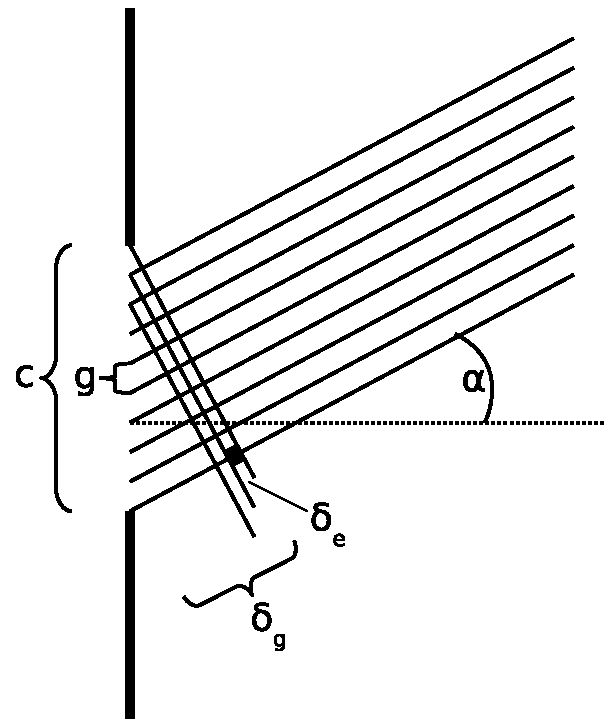
\includegraphics[width=0.5\textwidth]{mat/beugung_mehrfachspalt}
   \caption{Skizze zu Interferenz am Einzelspalt bzw. am Gitter}
   \label{img_aufbau_beugung_mehrfachspalt}
\end{figure}







	\section{Interferenz am Gitter}


\index{Beugung!Gitter}\index{Beugung!Mehrfachspalt}\index{Interferenz}Ein Gitter ist ein Mehrfachspalt. Die \textit{Gitterkonstannte} \(g\) gibt an, wie weit die Mittelpunkte zweier benachbarter Gitter auseinander liegen. Interferenz am Gitter funktioniert im Prinzip wie Interferenz am Einzelspalt, nur dass hier nicht unendlich viele Elementarwellen entstehen / interferrieren. Die Bedingungen für Minima und Maxima sind aus Kap. \ref{ss_beugung_doppelspalt} zu entnehmen. Betrachtet man Abbildung \ref{img_aufbau_beugung_mehrfachspalt}, so wird klar warum: der Gangunterschied \(\delta_e\) zwischen zwei einzelnen Spalten ist entscheidend dafür, ob die beiden Wellen einander auslöschen. Dieser ist dank der Definition der Gitterkonstante ebenso zu berechnen wie beim Doppelspalt.


Ein bedeutender Unterschied zwischen Beugung am Doppelspalt und Beutung am Gitter ist aber das entstehende Interferenzbild: Die einzelnen Maxima sind beim Gitter nämlich wesentlich weiter voneinander entfernt und außerdem schärfer. Vergleicht man Abbildung \ref{img_intensitaet_doppelspalt} und \ref{img_intensitaet_zehnerspalt} auf Seite \pageref{img_intensitaet_doppelspalt}, so ist dies ersichtlich. 

Die Erklärung für die vielen \emph{kleinen} Maxima ist dass hier die \(\vec{E}\) bei der Addition geschlossene Vektorzüge ("`Kreise"') bilden, die nichts produktives zur Intensität beitragen (siehe Formel \ref{eq_intensitaet}). Schärfer werden die Maxima dadurch, dass die Intensitäten schneller abfallen.


Für das Gitter gilt die selbe Einschränkung wie für den Doppelspalt: Die einzelnen Spalte fungieren jeweils als Einzelspalt, wodurch sich in einem realen Beugungsbild zwei verschiedene Phenomäne überlagern.







	\section{Spektrale Zerlegung}

Bisher wurde bei der Beugung nur eine einzige Farbe in Betracht gezogen ("`\textit{monochromatisches}"' Licht)\index{Monochromatisch}. Verwendet man bei einer Beugung jedoch Licht aus mehreren Farben\footnote{"`normales"', weißes Licht besteht aus vielen verschiedenen Farben}, so muss man die Maxima für die einzelnen Farben entsprechend berechnen. Es ergeben sich so in ein und dem selben Aufbau verschiedene Interferenzbilder für die verschiedenen Farben, die sich gegenseitig überlagern können.\index{Spektrale Zerlegung}








		\chapter{Brechung}

	\section{Beschreibung}

\index{Brechung}Bei der Brechung wird eine Welle beim Übergang in ein anderes Medium von seiner ursprünglichen Ausbreitungsrichtung abgelenkt. Diese Ablenkung basiert auf unterschiedlichen Ausbreitungsgeschwindigkeiten in unterschiedlichen Medien. Eine Begleiterscheinung ist die Reflexion.\index{Reflexion}

Grundsätzlich tritt Brechung bei verschiedenen Wellenformen auf, hauptsächlich spricht man jedoch im Bereich der Optik von Brechung. Im Allgemeinen sind die Angaben aber auch auf bspw. Erdbebenwellen zu beziehen.

Für den Einfallswinkel \(\alpha\) und den Ausfallswinkel \(\beta\)\index{Einfallswinkel}\index{Ausfallswinkel} -- beide gegenüber einem Lot\index{Lot} gemessen, welches senkrecht auf der Grenzfläche zwischen den Materealien steht -- gilt dabei der Zusammenhang:
\begin{equation}
   \frac{sin(\alpha)}{sin(\beta)} = \frac{n_2}{n_1} = n_{2,1} = \frac{c_1}{c_2}
   \label{eq_brechungsgesetz}
\end{equation}
Dabei sind \(n_M\) \emph{absolute} Brechzahlen\index{Brechzahlen}\index{Absolute Brechzahl} der Materealien \(M\): Das Verhältnis der Vakuumlichtgeschwindigkeit \(c_0\) zur Ausbreitungsgeschwindigkeit im Medium \(c_M\):
\begin{equation}
   n_M = \frac{c_0}{c_M}
   \label{eq_absoluter_brechungsindex}
\end{equation}
 \(n_{2,1}\) wird als \textit{relativer} Brechungsindex für den Übergang von Material 2 nach Material 1 bezeichnet.

Ist \(n_2 > n_1\) so spricht man bei \(M_2\) vom optisch \textit{dichteren}\index{Optisch dichter bzw. dünner} und bei \(M_1\) vom optisch \textit{dünneren} Medium. Im dichteren Medium pflanzt sich eine Welle langsamer fort und dementsprechend wird die Wellenlänge beim Übergang in ein optisch dichteres Medium kürzer.
 



	\section{\textsc{Huygens}}

\index{Huygen'sches Prinzip}Mit dem \textsc{Huygens}'schen Prinzip lassen sich sowohl Brechung als auch Reflexion anschaulich darstellen: Bei der Brechung breiten sich die von der Wellenfront am Materialübergang entstehenden Elementarwellen im optisch dichteren Medium langsamer aus, überlagern sich dann aber wieder zu einer Wellenfront. Verfolgt man parallel zu den sich im optisch dichteren Medium ausbreitenden Elementarwellen die, die sich weiterhin im optisch dünneren Medium ausbreiten, so erkennt man hier, dass sich diese Wellen zu einer reflektierten Wellenfront überlagern.


	\section{Totalreflexion}

\index{Totalreflexion}Allgemein gilt, dass der Lichtweg umkehrbar ist. Wird ein Lichtstrahl also in ein optisch dicheres Medium gebrochen und dort genau senkrecht reflektiert, so nimmt es genau den Weg, den es gekommen ist, wieder zurück. 

Fällt Licht jedoch unter einem Winkel von einem optisch dichteren Medium in ein optisch dünneres, sodass der Austrittswinkel rein rechnerisch über \(90^o\) liegen würde, so tritt \textit{Totalreflexion} auf. Der Einfallswinkel, bei dem dies stattfindet, wird als \textit{Grenzwinkel} \(\alpha_{grenz}\) bezeichnet.\index{Grenzwinkel} Normalerweise wird stets ein kleiner Anteil der Welle beim Übertritt in ein anders Medium reflektiert und dieser Anteil wächst, je größer der Einfallswinkel wird. Bei Totalreflexion wird die komplette Welle reflektiert und ins opitsch dichtere Medium zurückgeworfen.



	\section{Übergang dicht -- dichter}

Beim Übergang einer Welle von einem optisch dünneren in ein optisch dichteres Medium wird die Welle stets mit Phasensprung \(\Delta \varphi = \pi\) reflektiert, nur beim Übergang vom optisch dichteren ins optisch dünnere Medium erfolgt die Reflexion ohne Phasensprung.\index{Phasensprung}



	\section{Dispersion}

Als \textit{Dispersion}\index{Dispersion} bezeichnet man die Abhängigkeit des Brechungsindexes eines Materials von der Wellenlänge bzw. Frequenz des einfallenden Lichts. Je kurzwelliger bzw. hochfrequenter eine Welle ist, desto stärker wird sie gebrochen und desto größer ist folglich ihr Brechungsindex. Diese Eigenschaft macht man sich zunutze, um ein Spektrum zu erzeugen: In einem Prisma wird violettes Licht stärker gebrochen als rotes. Leuchtet man mit einem eng begrenzten weißen Lichtbündel auf ein Prisma, so erhält man dahinter ein (soweit die Farben im Weiß vorhanden waren) kontinuierliches Spektrum.





	\section{Spektrenvergleich}

\index{Spektrale Zerlegung!Vergleich Doppelspalt und Prisma}In Tabelle \ref{tab_spektrenvergleich} auf S. \pageref{tab_spektrenvergleich} werden wichtige Eigenschaften eines Spektrums vom Doppelspalt mit denen vom Prismenspektrum verglichen.

\begin{table}[h]
	\centering
	
   \begin{tabular}{l | l | l}
      ~ & \textbf{\textit{Gitter}} & \textbf{\textit{Prisma}} \\
      \hline
      \textit{Ursache} & Beugung durch Interferenz & Dispersion bei Brechung \\
      \textit{Farbanordnung} & Rot wird weiter weg abgelenkt & Blau wird stärker gebrochen\\
      \textit{Kontinuität} & mehrere Spektren neben- und übereinander & kontinuierliches Spektrum \\
      \textit{Anzahl} & mehrere Maxima je Farbe (möglich) & Jede Farbe nur einmal \\      
   \end{tabular}
\caption{Verglich der spektralen Zerlegung von Licht nach Beugung am Gitter und Brechung am Prisma}
\label{tab_spektrenvergleich}
\end{table}






		\chapter{Polarisation}

Als \textit{linear polarisiert}\index{Polarisation}\index{Linear polarisiert} bezeichnet man Licht, dessen E-Feld-Vektoren alle in einer Ebene schwingen. Somit lassen sich logischerweise nur Quer- bzw. Transversalwellen polarisieren.


	\section{EMW an Gitterstäben}

Eine linear polarisierte Elektromagnetische Welle kann ein metallenes Gitter nur dann passieren, wenn ihr \(\vec{E}\) senkrecht zu den Gitterstangen schwingt. Danntabular werden die Elektronen in den Stäben nämlich nicht zu starken Schwingungen angeregt (bzw. sie können aus Platzgründen nicht schwingen). Ist die Polarisationsebene jedoch parallel zu den Gitterstäben, so wird in den Stäben eine Schwingung erzwungen. Diese sorgt über ein kompliziertes Interferenzverfahren dafür, dass die Elektromagnetische Welle ausgelöscht wird.

Trifft eine solche Welle schräg auf ein Gitter, so kann stets nur der Teil -- also die Komponente -- das Gitter passieren, die senkrecht zu den Gitterstäben steht. Auf diese Weise wird die Polarisationsebene des Lichts geändert: Vorher war sie schräg zu den Gitterstäben, jetzt die "`überlebende"' Komponenten senkrecht zum Gitter ausgerichtet. Natürlich hat die Welle dabei an Intensität eingebüßt. Trifft eine Welle unter dem Winkel \(\alpha\) auf ein Gitter (\(\alpha\) bezeichnet den Winkel der Polarisationsebene mit dem Horizont bei lotrechten Gitterstäben), so kann nur ein Anteil \( \vert \vec{E}_a \vert \) weiterlaufen:
\begin{equation}
   \vert \vec{E}_a \vert = \vert \vec{E}_0 \vert \cdot sin(\alpha)
\end{equation}
Sind zwei Polarisationsfilter\index{Polarisationsfilter} parallel hintereinander aufgestellt mit senkrechten Polarisationsebenen, so dass normalerweise kein Licht hindurchgelangen könnte, so kann ein Anteil des Lichts die Filter passieren, wenn man noch einen dritten zwischen die beiden Filter stellt, dessen Polarisationsebene von denen der beiden anderen abweicht. Von einer Welle, die den ersten Filter passiert hat (\(\vert \vec{E}_a \vert\)), gelangt dann der Anteil \(\vert \vec{E}_d \vert\) durch den Aufbau, wenn der neue Polarisationsfilter mit dem Winkel \(\beta\) zum ersten steht:
\begin{equation}
   \vert \vec{E}_d \vert\ = \vert \vec{E}_a \vert \cdot \frac{1}{2} \cdot sin(2 \cdot \beta)
\end{equation}





	\section{Polarisation bei Brechungsvorgängen}

\index{Polarisation!Durch Brechung}Bei den folgenden Erklärungen sollte bedacht werden, dass eine Elektromagnetische Welle stets die Elektronen in ihrer Umgebung zu Schwingung anregt -- und zwar in Richtung ihres \(\vec{E}\). Fasst man die schwingenden Elektronen als Dipol auf, so kann dieser Dipol keine Welle parallel seiner Schwingungsrichtung / Längsachse ausstrahlen, sondern nur senkrecht dazu. Bei unpolarisiertem Licht schwingen die Elektronen also in alle Richtungen senkrecht zur Ausrbeitungsrichtung eines Lichtbündels.

	
		\subsection{Streuung}
		
\index{Polarisation!Durch Streuung}Wird ein Lichtbündel gestreut und ändert so seine Ausbreitungsrichtung um \(90^o\), kommen nur Elektronen in Frage, die sowohl senkrecht zur ehemaligen als auch zur neuen Ausbreitungsrichtung schwingen. Da nur diese eine Richtung in Frage kommt, schwingt das gestreute Licht auch nur in dieser Richtung -- ist also linear polarisiert.


		\subsection{\textsc{Brewster}-Winkel}

\index{Brewster-Winkel}\index{Polarisation!Brewster-Winkel}Stehen bei einer Brechung die Ausbreitungsrichtungen von reflektiertem und gebrochenem Lichtstrahl genau senkrecht aufeinander, so ist das reflektierte Licht völlig linear polarisiert. Es kommt nämlich auch hier nur eine einzige mögliche Richtung in Frage, in der die Elektronen Schwingen könnten, um einerseits noch in der vom gebrochenen Licht erzeugten Ebene zu schwingen und andererseits senkrecht zur neuen Ausbreitungsrichtung zu schwingen. 








		\chapter{Erdbeben - Kurzübersicht}


\index{Erdbeben}Durch tektonische Vorgänge können sich in der Erde Spannungen bilden, die sich dann bei einem Erdbeben lösen, wenn die Gesteinsschichten wegschnellen. Die Erde in der Umgebung des Epizentrums wird zum Mitschwingen angeregt. Ein Erdbebenzentrum liegt in \(30\) bis \(800 km\) Tiefe. Longitudinalwellen breiten sich mit \(c \approx 6 \frac{km}{h}\) in allen Richtungen aus, Transversalwellen folgen mit \(c \approx 3 \frac{km}{h}\), wobei diese sich nicht im flüssigen Erdkern weiter fortbewegen können. Große Zerstörungen verursachen dabei auch die von diesen beiden Wellen angeregten \textit{Oberflächenwellen}\index{Oberflächenwellen} an der Erdoberfläche mit starken Horizontalbeschleunigungen, die mit Frequenzen zwischen \(f \in [1;30] ~ Hz\) schwingen. Gebäude versucht man deshalb auch so zu bauen, dass sie in diesem Frequenzbereich keine Eigenfrequenz aufweisen.









		\chapter{Schallwellen}

\index{Schallwellen}Bei Schallwellen handelt es sich um \emph{Longitudinalwellen}\footnote{In Festkörpern können sie sich auch als Transversalwellen fortpflanzen.}. Hierbei schwingen die Massenteilchen längs der Ausbreitungsrichtung um eine Ruhelage. Dadurch entstehen Regionen erhöhten und verminderten Drucks. An Stellen maximalen \textit{(a)} und minimalen \textit{(b)} Drucks sind die Teilchen dabei in Ruhe, wobei ihre Schnelle \textit{(a)} in Richtung bzw. \textit{(b)} entgegen der Ausbreitungsrichtung wirkt.

Was in den vorangegangenen Kapiteln gesagt wurde, stimmt für Schallwellen auch weiterhin. Hier muss man allerdings bedenken, dass man Bei Schallwellen nicht eindeutig von \emph{Wellenbäuchen} sprechen kann. Wo nämlich ein \emph{Druck}bauch ist, sitzt gleichzeitig ein \emph{Schnellen}knoten.\footnote{Was man mit einem Mikrophon messen kann sind die Veränderungen des Luftdrucks}.\index{Druckbauch}\index{Schnellenbauch}

Die Ausbreitungsgeschwindigkeit \(c\) des Schallwellen ist dabei abhängig vom Ausbreitungsmedium\footnote{Luft: ca. \(340 \frac{m}{s}\); Wasser: ca. \(1485 \frac{m}{s}\); Eisen: ca. \(5200 \frac{m}{s}\)} und von der Temperatur, wobei der Luftdruck die Schallgeschwindigkeit nicht beeinflusst.


\subsubsection{Reflexionen, Überlagerungen \& Co}

\index{Reflexion}Schallwellen können an festen Gegenständen - wie bspw. Wänden - reflektiert werden. Dabei bildet sich an dem festen Gegenstand ein Schnellenknoten bzw. Druckbauch. In einem begrenzten Hohlkörper kann darüber hinaus noch zusätzlich Reflektion an einem offenen Ende geschehen; dann liegt am Offenen Ende ein Bewegungsbauch. Die Reflektion an einem festen Gegenstand entspricht dabei der an einem festen Ende, Reflektion an einem offenen Ende entspricht dabei der am losen Ende des Wellenträgers.









		\chapter{Elektromagnetische Wellen}


		\section{Dipol}

Lässt man in einem Schwingkreis\index{Schwingkreis} Ladungen schwingen, so wird gleichzeitig eine elektromagnetische Welle\index{Elektromagnetische Welle} emittiert.\footnote{Das bemerkt man bspw. wenn man einen Schwingkreis (mit richtiger Kapazität \(C\) und Induktivität \(L\)) in der Nähe eines Radios schließt - es wird im Radio ein Knacken zu hören sein.} Aus den \textsc{Thomson}'schen Schwingungsgleichungen ergibt sich dabei für die Frequenz, mit der der Schwingkreis schwingt und damit auch seine elektromagnetische Welle:
\begin{equation}
 	f_0 = \frac{1}{2 \cdot \pi \cdot \sqrt{C \cdot L}}
 	\label{freq_emw}
\end{equation}
Es handelt sich dabei um die \emph{Eigenfrequenz}\index{Eigenfrequenz} des Schwingkreises. Es ist also nicht alleine die Frequenz, bei der er seine elektromagnetische Strahlung aussendet, sondern auch die Frequenz, mit der er angeregt werden kann, wobei sich maximale Resonanz ergibt.




		\section{\textsc{Hertz}'scher Dipol}

\index{Hertz'scher Dipol}Um einen Dipol mit hohen Frequenzen anregen zu können, versucht man also die Werte für \(C\) und \(L\) möglichst \emph{klein} zu bekommen. Das gelingt, indem man einen Kondensator mit möglichst Breitem Plattenabstand und kleinen Plattenflächen nebst einer Spule mit wenig Querschnittsfläche, geringer Windungszahl und kleiner Länge verwendet. Verändert man einen Schwingkreis konsequent nach diesen Richtlinien, erhält man einen  \emph{\textsc{Hertz}'schen Dipol}. Er besteht aus einem schlichten Draht. Dabei übernehmen die Drahtenden die Funktionen der Kondensatorplatten und der Draht selbst fungiert als Spule.






		\section{Erregung des \textsc{Hertz}'schen Dipols durch EM Wellen}

Auf einem Empfangsdipol\index{Empfangsdipol} kann sich eine stehende Welle bilden, wenn seine Länge \(L\) mit Formel \ref{eq_2lose} über\-ein\-stimmt. Platziert man einen Verbraucher auf dem \textsc{Hertz}'schen Dipol, so muss man beachten, dass sich an manchen Stellen Strom- und an manchen Stellen Ladungsknoten bilden.\footnote{Ein Glimmlämpchen kann man so nicht in der Mitte eines Dipols der Länge \(L = \lambda\) zum Leuchten bringen, weil sich hier ein Stromknoten herausbildet und das Lämpchen Strom zum Leuchten bräuchte.}

An den Dipolenden ergeben sich Ladungsbäuche\index{Ladungsbauch}, weil sich hier schließlich die \textit{Kondensatorplatten} befinden, auf denen sich die Ladung komplett sammelt, wenn die komplette Energie der Schwingung in elektrischer Feldenergie vorliegt. Hat man einen Dipol, der länger ist als \(\frac{\lambda}{2}\), so ergeben sich auf der Länge des Dipols mehrere Stellen, an denen die Ladung sich zu Maxima 'sammelt' (s. Abb. \ref{img_Ix-Qx} auf S. \pageref{img_Ix-Qx})

Es ist dabei aber entscheidend, in welchem \emph{Medium} sich der Dipol befindet (\(\rightarrow\) Kap. \ref{ss_Ausbreitungsgeschwindigkeit} auf S. \pageref{ss_Ausbreitungsgeschwindigkeit}).


\begin{figure}
\centering
 \subfigure[I-x-Diagramm, \(L = \lambda\), \(t = 0\)]{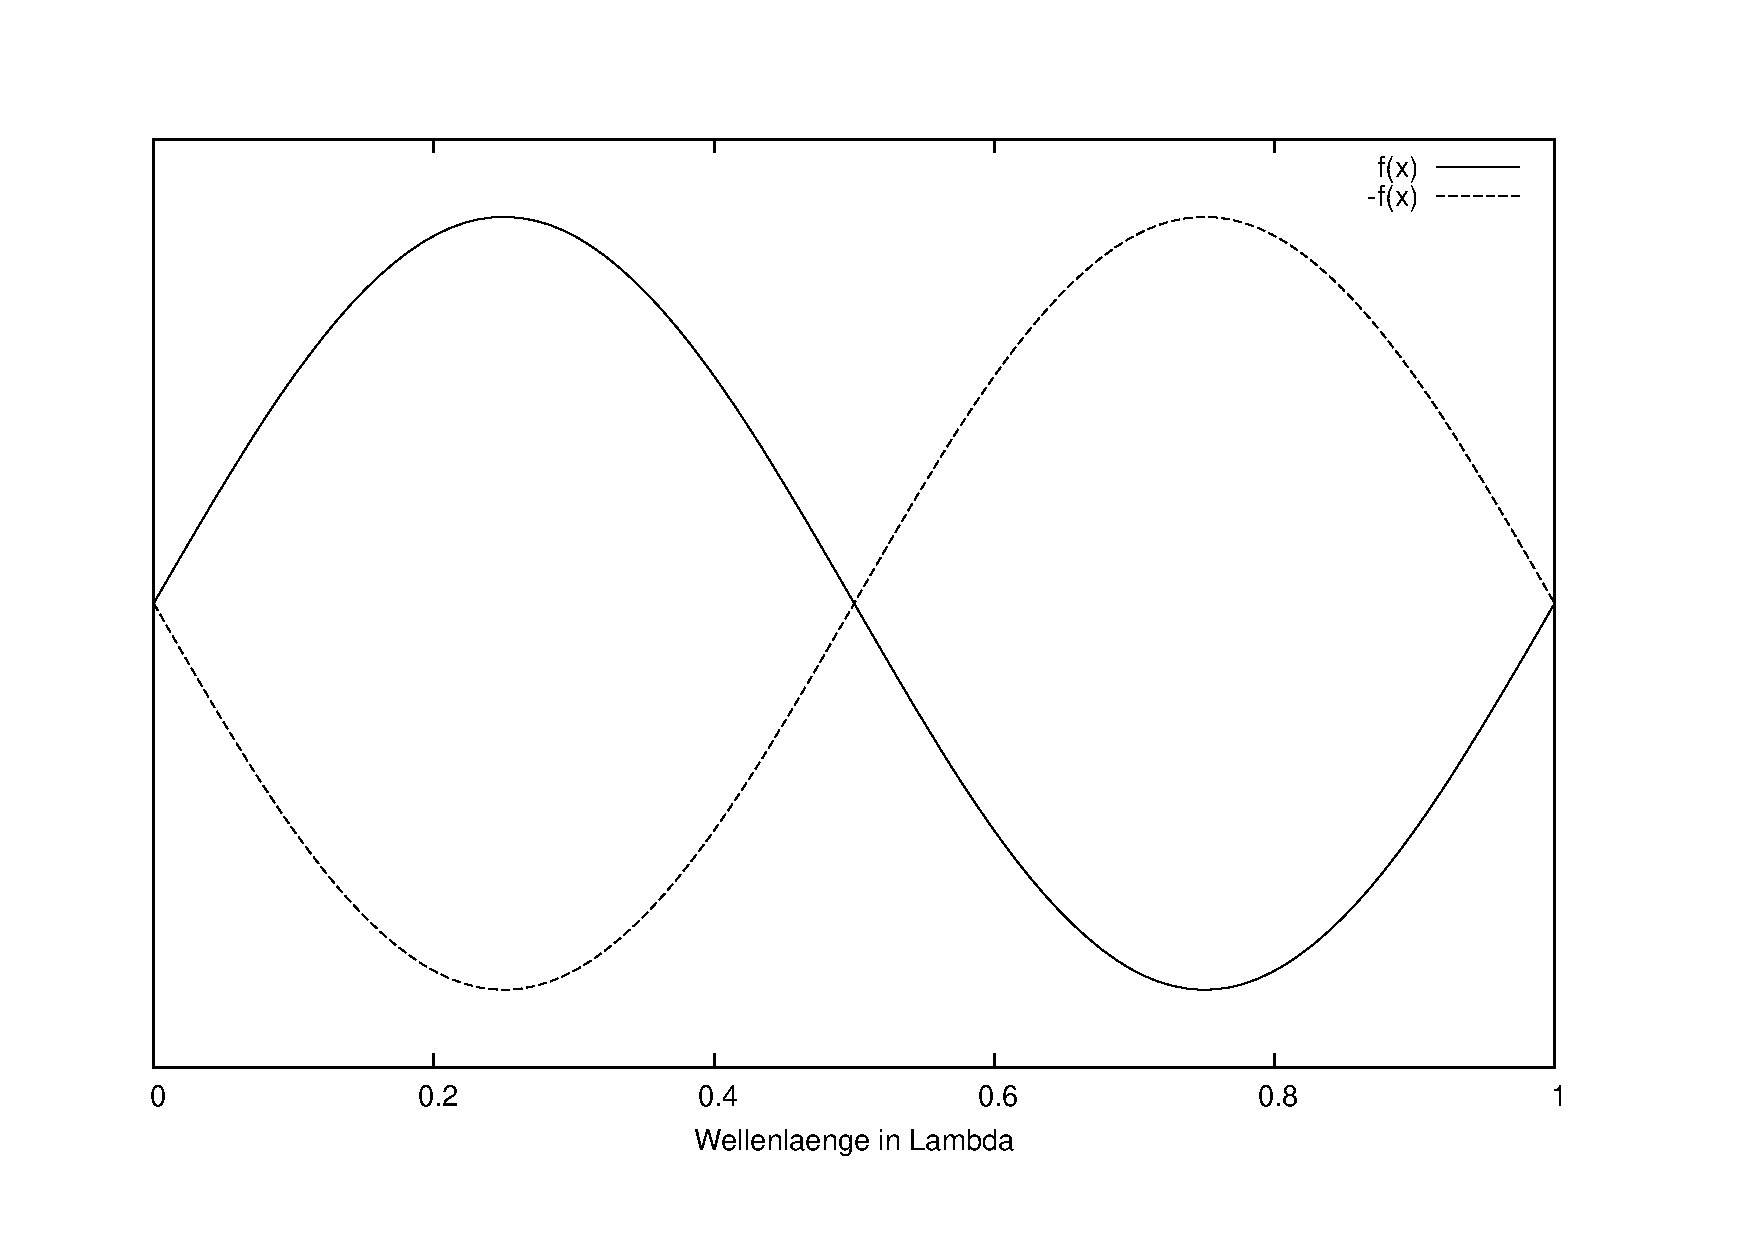
\includegraphics[width=0.4\textwidth]{mat/I10}}
 \subfigure[I-x-Diagramm, \(L = \frac{\lambda}{2}\), \(t = 0\)]{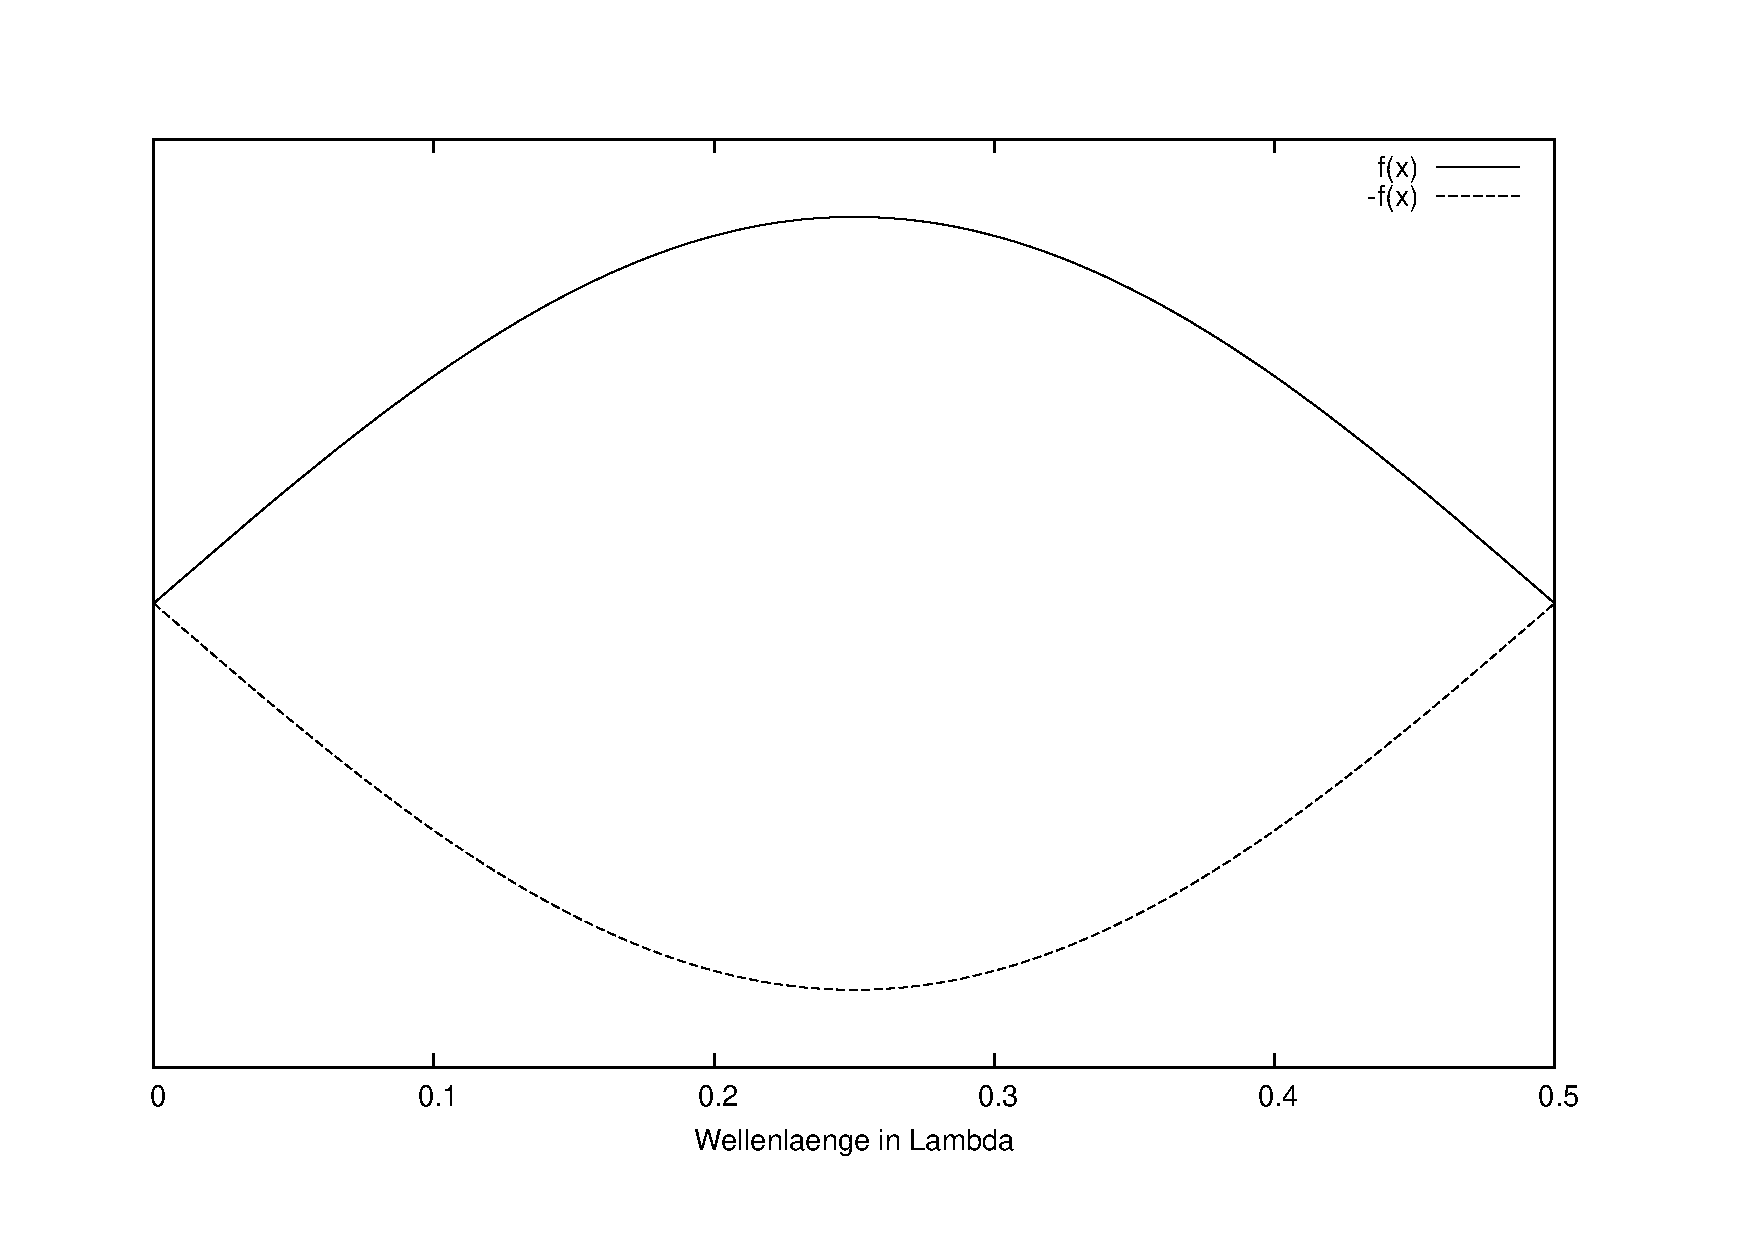
\includegraphics[width=0.4\textwidth]{mat/I05}}
 \subfigure[Q-x-Diagramm, \(L = \lambda\), \(t = \frac{T}{4}\)]{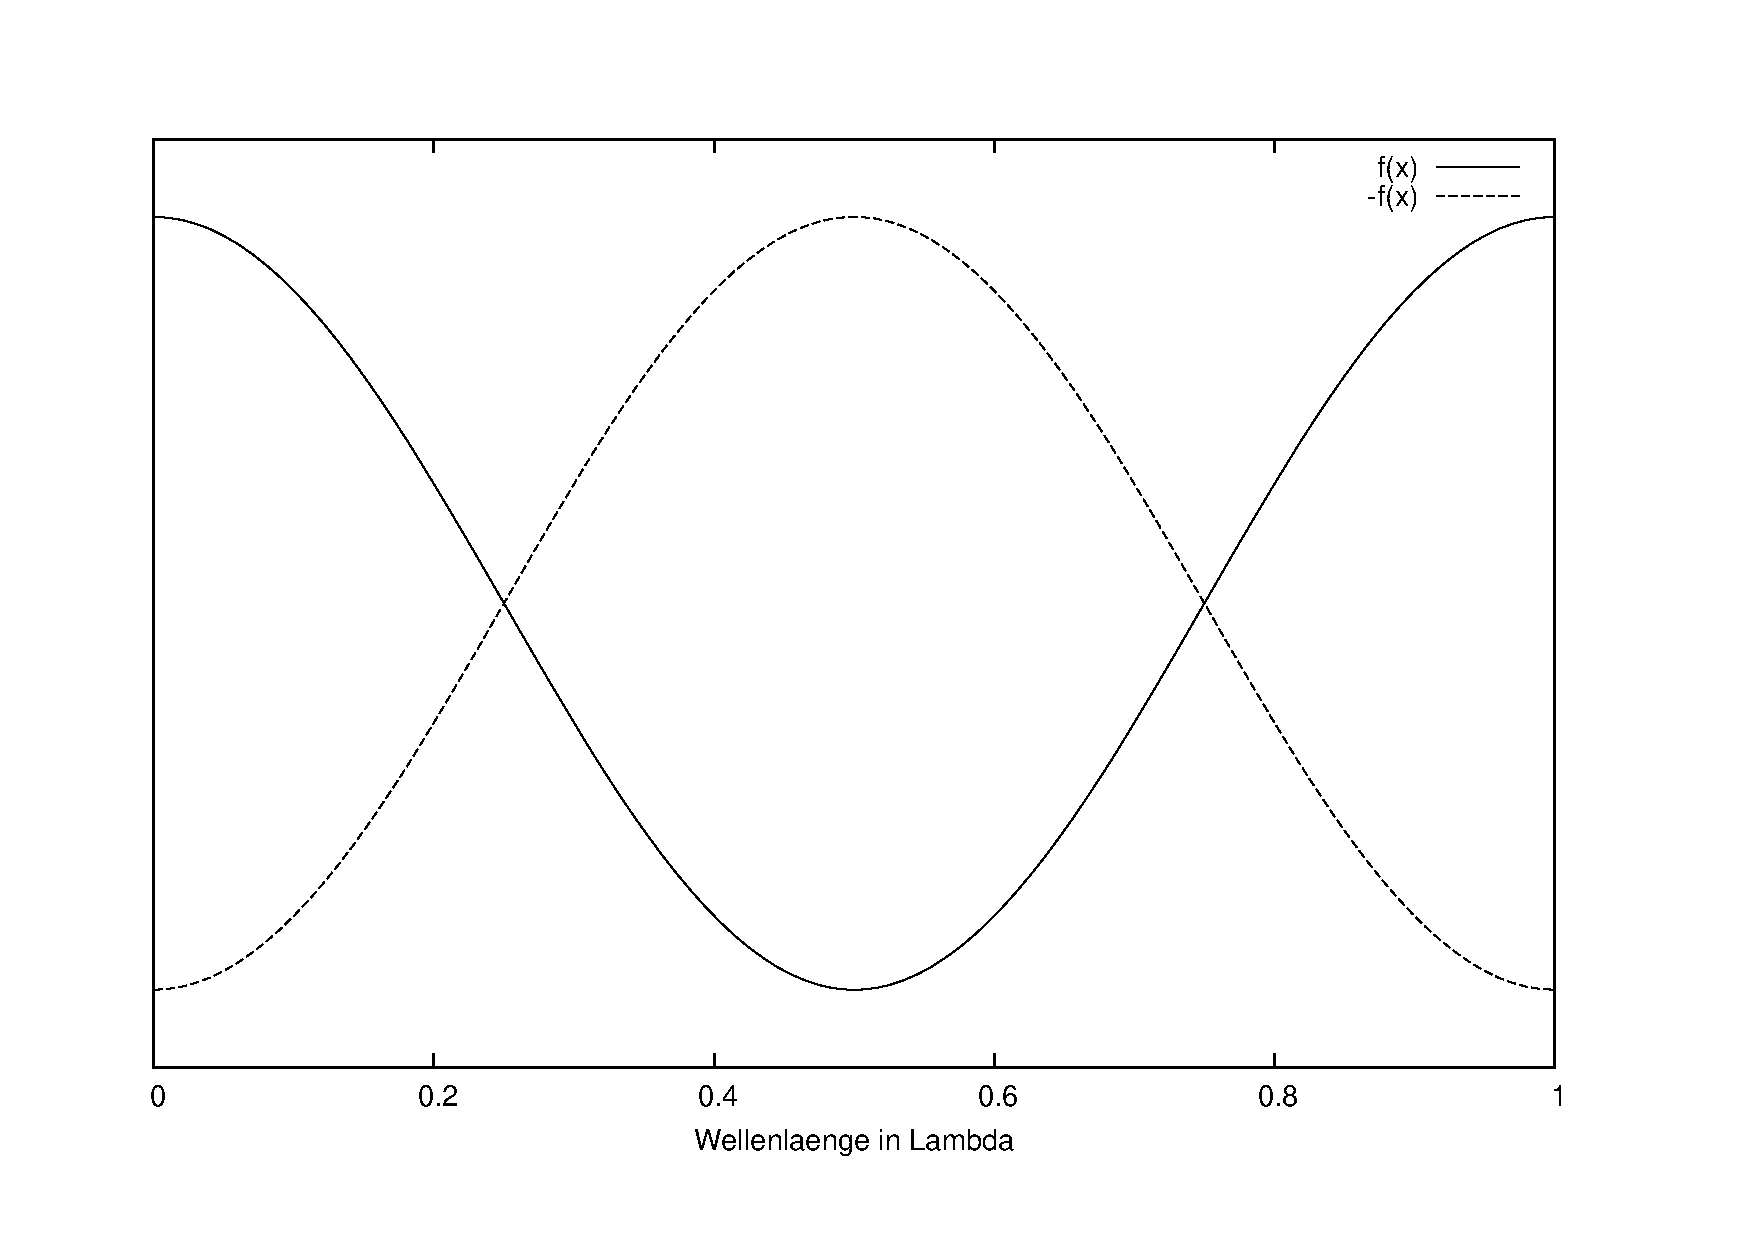
\includegraphics[width=0.4\textwidth]{mat/Q10}}
 \subfigure[Q-x-Diagramm, \(L = \frac{\lambda}{2}\), \(t = \frac{T}{4}\)]{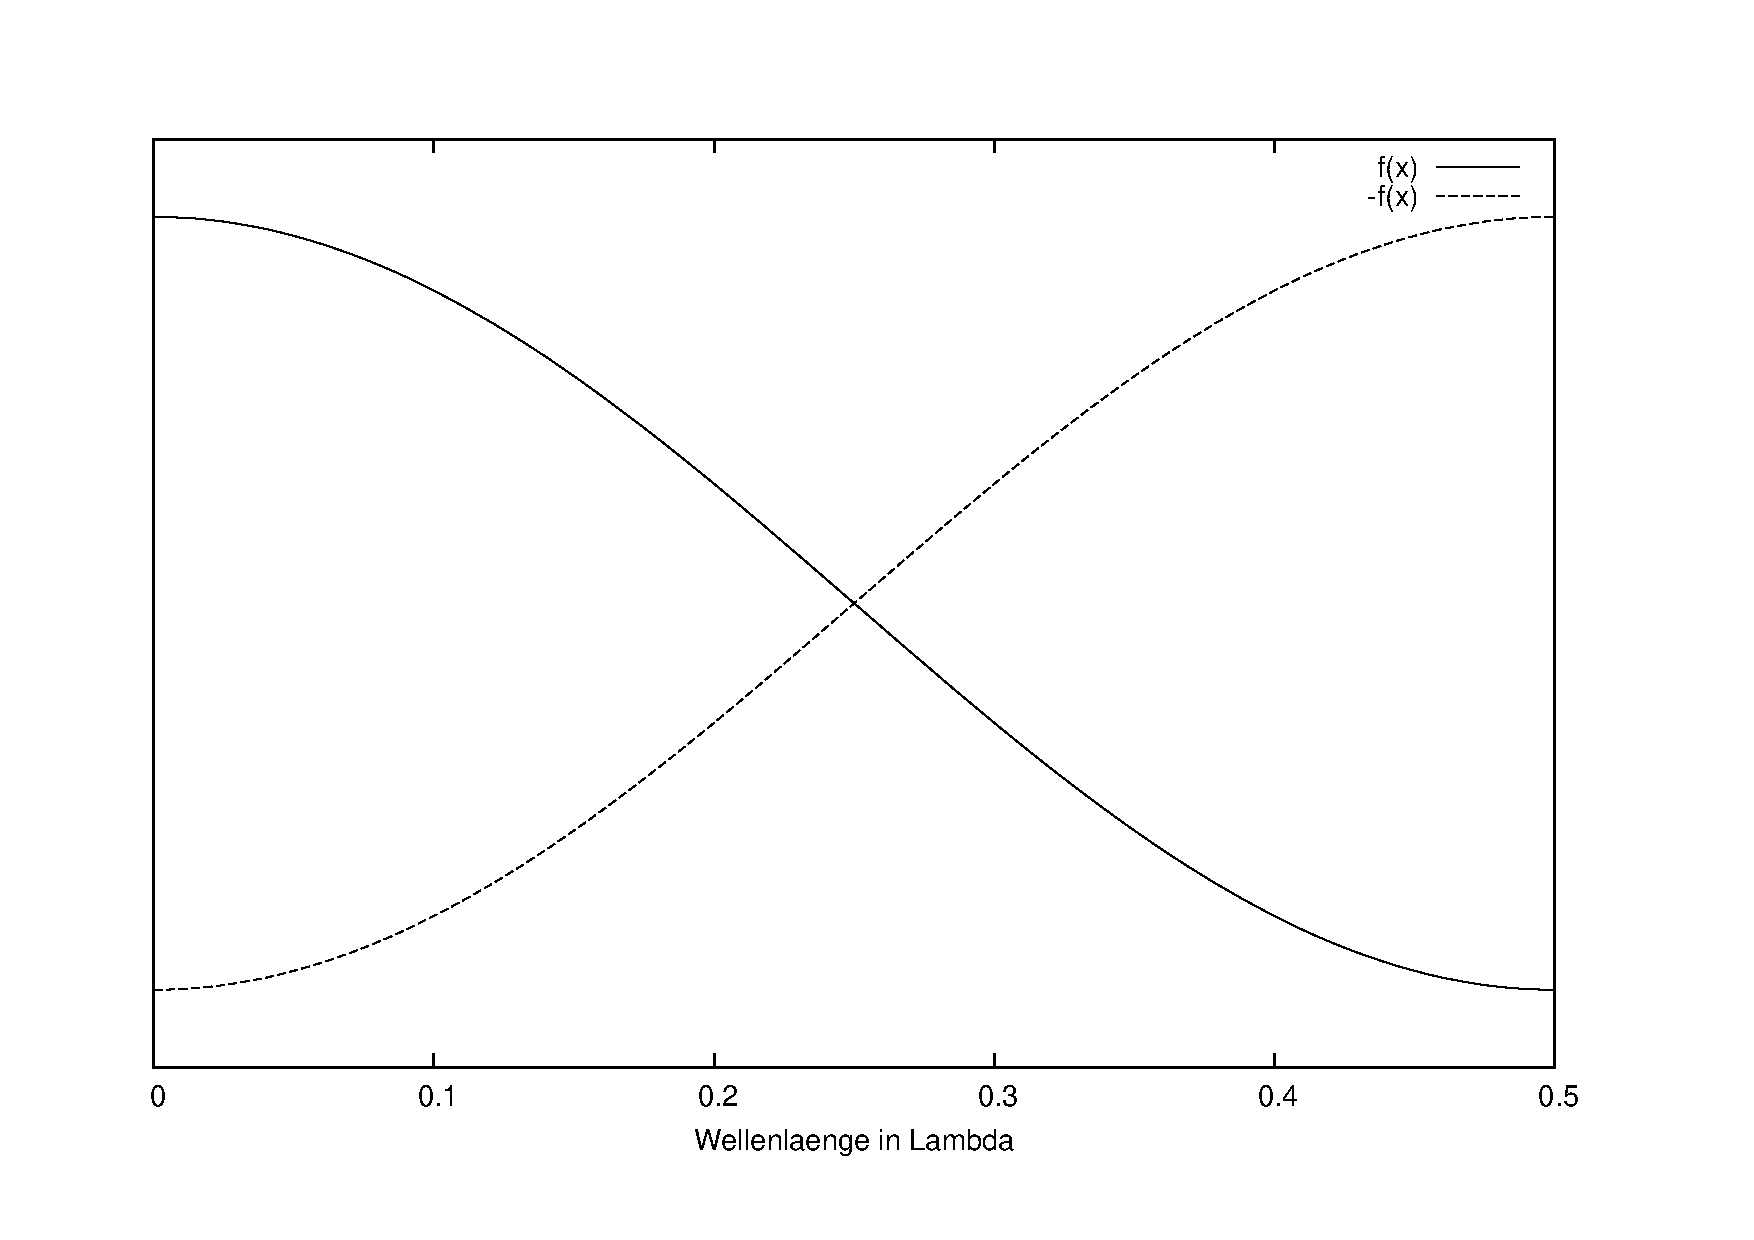
\includegraphics[width=0.4\textwidth]{mat/Q05}}
 	\caption{Stehende Wellen auf einem Empfangsdipol zu verschiedenen Zeiten; entweder Strom oder Ladung betrachtet}
 	\label{img_Ix-Qx}
\end{figure}






		\section{Definition Elektromagnetische Welle}

\index{Elektromagnetische Welle!Definition}Eine elektromagnetische Welle besteht aus einem B-Feld und einem E-Feld die sich durch ihre andauernden Änderungen stets gegenseitig 'erschaffen'. Dabei stehen B-Feld und E-Feld senkrecht aufeinander und gleichzeitig senkrecht zur Ausbreitungsrichtung, es handelt sich um eine \emph{Querwelle}.\footnote{Die von einem Dipol abgestrahlte elektromagnetische Welle ist \emph{linear polarisiert}. D.h., dass die Schwingungen senkrecht zur Ausbreitungsrichtung nur in \emph{einer} Richtung liegt. Außerdem strahlt der Dipol \emph{nicht} in Richtung seiner Achse.}
%Die Längen Vektoren der Felder schwingen dabei nach einer Sinus-Funktion.

Im Nahfeld eines \textsc{Hertz}'schen Dipols wird die Welle noch durch Ladungen und Ströme (mit)bestimmt, ab einer gewissen Entfernung - im \emph{Fernfeld} - jedoch erzeugen sich die Felder durch ihre zeitliche Änderung gegenseitig. Wäre dies nicht der Fall, so müsste die Intensität reziprok kubisch zur Entfernung abfallen\footnote{\(I \sim \frac{1}{r^3}\)} - das tut sie aber nicht. Die Schwingung im Dipol muss aber auch schnell genug sein, damit sich die Felder richtig abschnüren können, also in sich geschlossene Feldlinien bilden, die nicht mehr mit dem Dipol zusammenhängen.



		\section{Ausbreitungsgeschwindigkeit}
		\label{ss_Ausbreitungsgeschwindigkeit}

\index{Ausbreitungsgeschwindigkeit}Auch wenn elektromagnetische Wellen kein Medium brauchen, um sich fortzupflanzen, ist die \emph{Geschwindigkeit}, mit der sie sich fortbewegen vom umgebenden Medium abhängig. Die Frequenz einer Welle bleibt beim Übergang in ein anderes Medium unverändert. Durch die veränderte Ausbreitungsgeschwindigkeit und Formel \ref{eq_cLf} (S. \pageref{eq_cLf}) dagegen passt sich die Wellenlänge der Welle dem Medium an. Es gilt dabei für die Ausbreitungsgeschwindigkeit
\begin{equation}
 	c = \frac{1}{\sqrt{\mu_0 \cdot \mu_r \cdot \varepsilon_0 \cdot \varepsilon_r}}
\end{equation}





		\section{Reflexion und stehende Welle}

\index{Reflexion}Eine EM Welle wird an einer leitenden Wand reflektiert. Dabei baut sich in der Wand ein Gegen-E-Feld auf\footnote{\textsc{Lenz}'sche Regel: Das B-Feld der EM Welle induziert eine entgegengerichtete Spannung in der Wand.}. An dieser Stelle ist somit die Summe des E-Feldes \(\vec{0}\), es liegt also ein \emph{E-Feld-Knoten} vor. Durch die Ladungsverschiebung in der Wand ergibt sich wieder ein B-Feld und somit liegt an der Wand ein \emph{B-Feld-Bauch}.


Durch die Reflexion an der Metallwand ergibt sich logischerweise eine \emph{stehende Welle}, zumindest in direkter Nähe zur Reflexionsfläche. Bei ihr sind B-Feld und E-Feld um \(\Delta \varphi = \frac{\pi}{2}\) \emph{phasenverschoben}.




		\section{\textsc{Maxwell}gleichungen}

\index{Maxwell-Gleichungen}Für uns sind folgende Aussagen der \textsc{Maxwell}'schen Wellengleichungen wichtig:
\begin{itemize}
 \item Bewegt sich ein B-Feld mit der Geschwindigkeit \(v\), so erzeugt es ein E-Feld der Stärke \(E = B \cdot v\). Dieses E-Feld ist \emph{Ursache} der \textsc{Lorentz}-Kraft.
 
 \item Ein sich änderndes B-Feld erzeugt ein elektrisches Wirbelfeld
 
 \item Ein bewegtes E-Feld erzeugt ein B-Feld
 
 \item Ein sich änderndes E-Feld erzeugt ein magnetisches Wirbelfeld
\end{itemize}

Man kann sich die Richtungen der Felder jeweils (logisch) herleiten.\index{Rechte-Hand-Regel} Dazu kann man die rechte Hand verwenden und mit dem Daumen den Feldlinien eines E-Felds folgen, denn so man erhält aus der Richtung der Finger die Richtung des B-Feldes. Um das entstehende E-Feld zu bestimmen, verwendet man das \textsc{Lentz}'sche Gesetz: Wenn aus einem E-Feld ein B-Feld entsteht, so wird dieses stets in die Richtung zeigen, dass das aus \emph{ihm} entstehende E-Feld dem ersten - ursächlichen - E-Feld entgegensteht. D.h. Es muss ein B-Feld entstehen, dem man mit dem Daumen der Rechten Hand so folgen kann, dass die Finger der Rechten Hand dem bestehenden E-Feld entgegenzeigen. 
In dem Fall, dass ein B-Feld sich bewegt, kann man sich der Linken-Hand-Regel bedienen: Das E-Feld muss so entstehen, dass Elektronen in ihm der \textsc{Lorentz}-Kraft folgen würden.






%\cleardoublepage
\part{Quantenphysik}


\chapter{Definitionen}


\section{Quantenphysik ?!}

Die \emph{Quantenphysik}\index{Quantenphysik} beschreibt das Verhalten von Teilchen auf atomarer Ebene und tiefer. Eine besondere Eigenschaft ist dabei, dass bestimmte Größen \emph{gequantelt}\index{gequantelt} vorkommen -- also nur bestimmte, diekrete Größen haben können. Das \textsc{Planck}'sche Wirkungsquantum $h$\index{Plakck'sches Wirkungsquantum}\index{Wirkungsquantum} ist eine bedeutende Konstante in der Quantenphysik.

In der Quantenphysik können über bestimmte Eigenschaften der beobachteten Objekte keine Aussagen gemacht werden. Bspw. kann man bei einem Quantenobjekt nicht sagen, wie es einen bestimmten Weg zurücklegt. Außerdem lassen sich manche Größen nicht beliebig genau messen. Bei Impuls \(p\) und Ort \(x\) eines Teilchens beispielsweise hängt die Messgenauigkeit der einen Größe von der Genauigkeit bei der zweiten Größe ab.

Als mathematischen Formalismus, mit dem man das Verhalten der Teilchen recht genau vorhersagen kann, dient die Zuordnung einer \emph{Wahrscheinlichkeitswelle} $\Psi(x)$\index{Wahrscheinlichkeitswelle} zu jedem bestimmten Teilchen. Ihr Quadrat $\Psi^2$\index{Psi ($\Psi$)} ist die Wahrscheinlichkeit, das Teilchen am betreffenden Punkt anzutreffen.

Insgesammt richtet es sich in der Quantenphysik oft nach Wahrscheinlichkeiten....


\section{Wesenszüge der Quantenmechanik}

\begin{description}
   \item[Statistisches Verhalten] Man kann für ein einzelnes Teilchen nicht ausrechnen, wo es auftreffen wird, sondern nur eine Wahrscheinlichkeit dafür. Wiederholt man einen Versuch oft genug, wo werden viele Teilchen sich an diese Wahrscheinlichkeitsverteilung halten.\index{Wahrscheinlichkeitsverteilung} Abgesehen von stochastischen Abweichungen ist dann die Verteilung der angetroffenen Teilchen gleich der berechneten Aufenthaltswahrscheinlichkeit.
   \item[Interferenzfähigkeit] Einzelne Quantenobjekti können mit sich selbst interferieren. Voraussetzung dafür ist, dass es für den Weg mehrere (klassische) Möglichkeiten gibt. Auf diesem Weg interferieren nun die Wahrscheinlichkeitswellen miteinander und erzeugen die Auftreffwarhscheinlichkeit.\index{Interferenz!Wahrscheinlichkeitswellen}\index{Interferenz!Quanten}
   \item[Objektiv unbestimmbar] Bei mehreren (klassischen) Wegmöglichkeiten zur realisierung eines Zustands ist es nicht möglich, zu sagen, welchen das Quantenteilchen auch wirklich eingeschlagen hat. Vielmehr hat es schlichtweg \emph{keinen} der möglichen Wege realisiert. Im Bezug auf manche Größen ist es nicht möglich sie einem Quantenteilchen zuzuordnen.
   \item[Eindeutige Messung] Wenn mehrere (klassische) Möglichkeiten vorliegen, ist es möglich, zu messen, welche dieser Möglichkeiten das Quantenobjekt realisiert, indem man es durch die Messung in den klassischen Zustand drängt. Man misst also nicht mehr die Eigenschaft des Quantenobjekts, weil dieses ja keinen der zu messenden Zustände realisiert hat.
   \item[Komplementarität]\index{Komplementarität} \emph{Wegen} dieser Messung wird das Quantenteilchen sich von nun an aber wie ein klassisches Teilchen verhalten. Es wurde gewissermaßen "`gezwungen"', einen klassischen Zustand zu realisieren und verbleibt dann in diesem. Man kann also entweder messen, wo sich ein Teilchen aufhält oder seine Quanteneigenschaften -- wie bspw. Interferenz -- beobachten.
 \end{description}



\chapter{Interferenz}



	\section{Messung unbestimmter Methoden}


\subsubsection{Messungen auf beiden möglichen Wegen}
Wenn auch ein Wesenszug der Quantenmechanik besagt, dass das Teilchen sich an einem unbestimmten Ort aufhält, so kann man diesen genau bestimmen -- so ein weiterer Wesenszug. Misst man, wo sich ein Quantenteilchen aufhält, so bekommt man dafür eine genaue Information. Diese Information kann nun dazu führen, dass Interferenz (bspw. am Doppelspalt) unterbunden wird.

Schickt man Quantenteilchen auf einen Einzelspalt, so findet dort Beugung am Einzelspalt statt.\footnote{Die effektive Spaltbreite -- auf die man durch Untersuchung des Interferenzbildes schließe -- ist jedoch auch abhängig von der Wellenlänge: Nur wenn die max. Auflösung den kompletten Spalt abdeckt, findet die INterferenz am Einfachspalt ungestört statt.}\index{Beugung!Quanten} Schickt man die Quantenobjekte dagegen -- unbeobachtet -- auf einen Doppelspalt, so ergibt sich Interferenz am Doppelspalt. Interessant ist dabei, dass die Elektronen weder den Weg durch den einen noch durch den anderen Spalt wählen und es trotzdem zu Interferenz zwsischen den $\Psi$-Wellen der beiden klassisch möglichen Wege kommt.

Setzt man nun jedoch Messinstrumente ein, mit denen man \emph{theoretisch}\footnote{Die Einschränkung kommt daher, dass man wie beim "`Quantenradierer"' in jeden Spalt des Doppelspalts je eine Polarisationsfolie einbringt, wobei die beiden Polarisationswinkel sich um $90^o$ unterscheiden. Es ist danach das Interferenzbild von der Beugung am Einzelspalt zu beobachten, weil man durch bestimmte Geräte unterscheiden könnte, durch welchen Spalt die Quantenteilchen gelangt sind, auch wenn man bei normaler Beobachtung nicht darauf schließen kann (weil wir ja kein unterschiedlich polarisiertes Licht unterscheiden können).} unterscheiden kann, durch welchen der beiden Spalten das Quantenobjekt gegangen ist, zwingt man es gewissermaßen dazu, sich zu entscheiden, durch welchen der beiden Spalte es gehen möchte. Ohne die Messinstrumente kann es eine Art "`Zaubertrick"' rund um und durch den Doppelspalt aufführen, dessen Effekt die Interferenz ist. Nun zwingt man es dagegen, sich zu entscheiden, welchen Spalt es nehmen möchte. Damit ist das Interferenzbild des Doppelspaltes ausgeschlossen, weil dazu \emph{beide} Spalte einbezogen werden müssen -- es muss \emph{Irgendetwas} aus jedem der beiden Spalte zu der Beugung beitragen. Wird das Quantenteilchen dagegen gezwungen, einen der beiden Wege zu nehmen, kann es nicht gleichzeitig noch den zweiten Weg mitbenutzen -- was ja nötig gewesen wäre, um Interferenz am Doppelspalt zu erhalten.




	\subsubsection{Messung auf einem möglichen Weg}

Seltsam wird die Sache allerdings dadurch, dass der oben beschriebene Effekt auch dann eintritt, wenn nur einer der beiden Wege überwacht wird. Geht man wieder von Interferenz am Doppelspalt aus und überwacht nur \emph{einen der beiden} Spalten auf passierende Elektronen, so wird sich auf dem Schirm trotzdem das Interferenzbild von der Beugung am Einzelspalt zeigen.

Bei zwei Wegen -- A und B -- wird nur der Weg A überwacht. \emph{Trotzdem} wird ein Teilchen gezwungen, sich zwischen den beiden Wege zu entscheiden. Nimmt ein Teilchen den Weg B, so kann es eigentlich nicht wissen, dass Weg A überwacht wird. Trotzdem lässt es sich von der Überwachung auf Weg A in das "`klassische Schema"' drücken und verliert dadurch seine Fähigkeit, den "`Zaubertrick der Interferenz"' zu vollführen.






	\subsubsection{Messung beider Wege die danach zurückgenommen wird}

Beim oben angesprochenen "`Quantenradierer"'\index{Quantenradierer} kann man nun eine weitere Polarisationsfolie einbringen. Sie wird zwischen (präpariertem) Doppelspalt und Schrim eingebracht und ihr Polarisationswinkel steht im Winkel von $44^o$ auf den Winkeln der beiden Folien in den Spalten.

\index{Polarisation}Licht, das von den Folien in den Spalten polarisiert wurde, muss nun, um auf den Schirm zu gelangen, auch diesen Filter passieren. Dabei kommen von dem Licht, das vorher in zwei senkrecht zueinander stehenden Ebenen polarisiert war, nur diejenigen Anteile durch, die im Winkel von $45^o$ zu den beiden Ebenen liegen. Nach diesem dritten Polarisationsfilter ist also alles licht wieder in die selbe Richtung (in der selben Ebene) polarisiert.

Das Licht aus den beiden Spalten hat darüber hinaus die selbe Intensität -- durch die beiden Spalte fällt die selbe Lichtmenge. Nach dem dritten Polarisationsfilter ist also nicht mehr entscheidbar, welchen der beiden Spalte das Licht passiert hat und somit ergibt sich wieder Interferenz am Doppelspalt mit dem dazugehörigen Schirmbild. Die Quantenteilchen müssen sich also am Doppelspalt nicht mehr entscheiden, weil sie "`wussten"', dass \emph{hinter} dem Spalt ein weiterer Filter kommt, durch den nicht mehr entscheidbar ist, welchen Weg sie wählten -- und dadurch mussten sie nicht mehr wählen. 


\subsubsection{Das Verwirrende also:} Die Quantenteilchen können somit also gewissermaßen in die Zukunft blicken, bzw. den Weg sehen, den sie \emph{nicht} genommen haben.










\section{Abhängigkeit von Wellenlänge des Lichts, mit dem beobachtet wird}

Interferenz tritt nur dann auf, wenn das Teilchen unbeobachtet ist -- sich also gewissermaßen ungestört als Quantenobjekt aufführen kann. So lange nimmt es keinen besonderen Weg und seine $\Psi$-Wellen können ungestört interferieren. Will man jedoch unterscheiden, welchen Weg das Teilchen nimmt, so kann es nicht mehr als Quantenteilchen "`handeln"' und wird gezwungenermaßen zum klassisch\emph{eren} Teilchen.

Damit es sich wie ein vollständig klassisches Teilchen verhält, müsste man unendlich genau beobachten, welchen Weg es nimmt. Da die Messung aber mit Licht funktioniert, ist der Genauigkeit der Ortsbestimmung durch die optische Auflösung Grenzen gesetzt. Mit Licht der Wellenlänge $\lambda$ kann man nämlich nur entscheiden, dass sich das Quantenteilchen im Bereich $\frac{1}{2} \lambda$ irgendwo aufgehalten hat.

% Beleuchtet man so also einen Doppelspalt, um herauszubekommen, aus welchem der beiden Spalte bspw. ein Elektron geflogen kommt und verwendet dazu Licht einer Wellenlänge die kleiner als der Abstand zwischen den beiden \emph{äußeren} Spaltenden ist ("`Spaltaußenabstand"'), so wird man auf dem Schirm stets ein Interferenzbild erhalten, das nach Interferenz am \emph{Einzelspalt} aussieht. Die Elektronen können nämlich nicht aufgelöst werden, aus welchem Spalt sie kommen und somit kann sich ungestört Interferenz am Doppelspalt für jedes einzelne Teilchen ergeben.
% 
% Senkt man nun jedoch die Wellenlänge des Lichts ab, sodass sie kleiner ist als der Spaltaußenabstand, so kann man mehr und mehr unterscheiden, aus welchem Spalt ein Elektron kommt. Ist die Wellenlänge nur wenig kleiner als der Spaltaußenabstand, so 

\index{Interferenz!Quanten}Es ergibt sich der Zusammenhang (Daten siehe Tab. \ref{tab_daten_lambda_0}) zwischen Spaltabstand $g$, Spaltbreite $l$ und Wellenlänge $\lambda_0$, unterhalb der sich nurnoch Interferenz am Einzelspalt ergibt:
\begin{equation}
   2 \cdot g - 2 \cdot l = 2 \cdot (g - l) = \lambda_0
\end{equation}
Damit entspricht die Wellenlänge $\lambda_0$ dem Doppelten des "`Balkens"' zwischen den beiden Spalten des Doppelspalts. Oberhalb dieser Wellenlänge erhält man teilweise das Interferenzbild am Doppelspalt. Das volle Bild des Doppelspalts\footnote{Definitionsgemäß wurde das angenommen, sobald die totalen Minima um das erste Hauptmaxima die Intensität $0$ hatten.} erhält man dagegen (Daten siehe Tab. \ref{tab_daten_lambda_1}) erst mit Licht der Wellenlänge $\lambda_1$:
\begin{equation}
   2 \cdot g = \lambda_1
\end{equation}
Erklären kann man sich diese Zusammenhänge dadurch, dass die Auflösung einer Lichtwelle durch deren Wellenlänge festgelegt ist -- und zwar ist die maximale Auflösungslänge gleich der Hälfte der Wellenlänge. Das würde auch zur \textsc{Abbe}'schen Abbildungsbedingung (für Lichtmikroskope) passen. Sie sagt, die Max. Auflösung $d = \frac{\lambda}{2 \cdot n \cdot sin(\alpha)}$. Da wir kein Mikroskop mit beschränkung haben, ergibt sich für unsere Beobachtung der Winkel $\alpha = 90^o$, da wir in Luft arbeiten ergibt sich $n \approx 1$ und somit $d = \frac{\lambda}{2}$.\index{Auflösung}\index{Abbe'sche Abbildungsbedingungen}

\index{Beobachtung von Quanten}Sobald nun die Auflösung kleiner ist als der Steg zwischen den beiden Spalten, ist es auf keinen Fall mehr möglich, beide Spalte mit dem selben Lichtblitz zu beobachten. Wäre die Wellenlänge ein klein bisschen größer, könnte es im ungünstigsten Falle sein, dass die Lichtwelle genau auf die Spaltmitte fällt und somit von beiden Spalten einen Teil betrachtet -- nun könnte ein Elektron also weiterhin durch beide Spalte gleichzeitig gelangen und würde trotzdem von der selben Welle registriert. Erst wenn $\lambda < \lambda_0$ gilt, ist dies ausgeschlossen und es kann immer nur ein Spalt gleichzeitig beobachtet werden. Somit ist absolut klar, aus welchem Spalt das Elektron geflogen kam und somit ist Interferenz zwischen einem Elektron mit sich selbst aus zwei verschiedenen Spalten völlig ausgeschlossen.

Bei größerer Wellenlänge ($\lambda_0 < \lambda < \lambda_1$) ist es nun für Elektronen möglich, immernoch beide Spalte zu passieren und trotzdem von dem selben Lichtblitz wahrgenommen zu werden. Ist $\lambda$ nur geringfügig größer als $\lambda_0$, so ist es wenig wahrscheinlich, dass ein Elektron dieses Kunststück zu Werke bringt. Hier überlagern sich die beiden Fälle von Interferenz: Einmal am Doppelspalt von sehr wenigen Elektronen und einmal am Einzelspalt von sehr vielen Elektronen. Das Bild sieht deshalb noch weitgehend aus wie bei Beugung am Einzelspalt. Je mehr sich $\lambda$ dann $\lambda_1$ annährt, desto mehr Elektronen ist es möglich, das Kunststück zu vollführen.

Wenn dann $\lambda > \lambda_1$ ist ein neuer Fall der totalen Unkontrollierbarkeit eingetreten: Es ist jetzt überhaupt nicht mehr möglich, zu entscheiden, aus welchem Spalt ein bestimmtes Elektron gekommen ist -- und folglich entsteht ab jetzt ein Interferenzbild des Doppelspalts auf dem Schirm. 

~\\Was man die ganze Zeit über beachten muss ist, dass $\lambda < l$ gelten müsste, damit die Interferenz am Einfachspalt ebenfalls eingeschränkt wird. Es ergibt sich daraus eine neue Grenzwellenlänge:
\begin{equation}
   2 \cdot l = \lambda_2
\end{equation}
Unterhalb dieser Wellenlänge ergibt sich nurnoch Interferenz am Einzelspalt, außerdem sieht das interferenzbild so aus, als ob der Spalt nur $l' = \frac{\lambda}{2}$ breit ist.




\begin{table}
\centering
\subtable[
	Bestimmung von $\lambda_0$
]{
	\begin{tabular}{c c c}
	%Spaltabstand [nm] & Spaltbreite [nm] & vollst. Einzelspaltinterferenz unterhalb Wellenlänge [nm]\\
	$g$ [nm]& $l$ [nm]& $\lambda_0$[nm]\\
	400	&	100	&	600\\
	400	&	150	&	500\\
	400	&	200	&	400\\
	300	&	100	&	400\\
	350	&	100	&	500\\
	400	&	100	&	600\\
	450	&	100	&	700
	\end{tabular}\label{tab_daten_lambda_0}
}
\subtable[
	Bestimmung von $\lambda_1$
]{
	\begin{tabular}{c c c}
		%Spaltabstand [nm] & Spaltbreite [nm] & vollst. Doppelspaltinterferenz oberhalb Wellenlänge [nm]\\
		$g$ [nm]& $l$ [nm]& $\lambda_1$[nm]\\
		
		250 & 100 & 500\\
		275 & 100 & 550\\
		300 & 100 & 600\\
		325 & 100 & 650\\
		350 & 100 & 700\\
		250 & 100 & 500\\
		200 & 200 & 400\\
		250 & 125 & 500\\
		250 & 150 & 500\\
		300 & 100 & 600\\
		300 & 125 & 600\\
		300 & 150 & 600\\
		300 & 200 & 600
	\end{tabular}\label{tab_daten_lambda_1}
}
\caption{Ergebnisse aus Versuchen mit Elektronen $\lambda_{Elektron} = 4pm$}
\label{tab_versuch_zshg_spalten_wellenlaenge}

\end{table}




















\chapter{Mathematischer Formalismus}

Um das Verhalten von Quantenteilchen vorherzusagen, ordnet man ihnen eine $\Psi$-Welle\index{Psi ($\Psi$)}\index{Psi ($\Psi$)!Psi-Welle} zu. Dazu ordnet man jedem Teilchen, abhängig von Seiner Energie $W$, eine Wellenlänge zu. Um die Welle aufzustellen bekommt deswegen auch ein Elektron eine Wellenlänge. Diese "`\textsc{DeBroglie}-Wellenlänge"'\index{DeBroglie-Wellenlänge} berechnet sich nach
\begin{equation}
   \lambda = \frac{h}{m \cdot v} = \frac{h}{p}
   \label{eq_debroglie}
\end{equation}
Um die Welle mathematisch auszudrücken benötigt man jedoch \emph{Komplexe Zahlen}.\index{Komplexe Zahlen} Man kann sich für die Funktion einen rotierenden Zeiger denken, dessen $y$-Komponente imaginär und dessen $x$-Komponente reell ist. Da die Amplitude des Zeigers jedoch konstant ist, ist auch die Aufenthaltswahrscheinlichkeit $\Psi^2$ eines Teilchens entlang einem rotierenden "`Zeigerstrahl"' konstannt.
Für $\Psi(x)$ ergibt sich:
\begin{equation}
   \Psi(x) = \Psi_0 \cdot cos(\varphi_x) + \Psi_0 \cdot i \cdot sin(\varphi_x) = \Psi_0 \cdot cos \left( \frac{2 \pi \cdot x}{\lambda} \right) + \Psi_0 \cdot i \cdot sin \left( \frac{2 \pi \cdot x}{\lambda} \right)
   \label{eq_psi(x)}
\end{equation}
Nach der Zeit $t$ müssen alle Zeiger um den Betrag $\varphi_t = \frac{2\pi \cdot t}{T}$ "`zurückgedreht"' werden, um wieder auf die durch Formel \ref{eq_psi(x)} gebracht zu werden. Dadurch ergibt sich eine Phase für jeden Zeiger von $\varphi = \varphi_x - \varphi_t$ und damit für die Wellengleichung:
\begin{equation}
   \Psi(x,t) = \Psi_0 \cdot  cos \left(\frac{2\pi\cdot x}{\lambda} - \frac{2\pi \cdot t}{T}\right) + \Psi_0 \cdot i \cdot sin \left(\frac{2\pi\cdot x}{\lambda} - \frac{2\pi \cdot t}{T} \right)
\end{equation}
\index{Wellengleichung!Quanten}Über diese Wellengleichungen kann man nun Interferenzen der Teilchen berechnen. Interessant ist dabei, dass man die Interferenzen von einzelnen Teilchen \emph{mit sich selbst} berechnet. Um ein messbares Ergebnis zu erhalten addiert man die $\Psi$-Wellen zur Zeit $t_0$ am Ort $x_0$ wie gewohnt um dann die Auftreffwahrscheinlichkeit eines einzelnen Teilchens mit $\Psi_{sum}^2(x_0,t_0)$ zu berechnen.






\chapter{Abweichungen von Klassischen Vorstellungen}



\section{Photoeffekt}


\subsubsection{Versuchsdurchführung}

%\subsubsection{Photoeffekt}

\index{Photoeffekt}Eine Metallplatte wird mit monochromatischem Licht bestrahlt. Vor der Metallplatte sitzt ein leitender Ring, durch den das Licht einfällt. Zwischen dem Ring und der Metallplatte wird eine Spannung $U_A$ angelegt und die Stromstärke gemessen. Die Spannung wird während des Versuchs für jede Frequenz so lange erhöht, bis gerade keine Stromstärke mehr zu messen ist. Dann ist die Spannung $U_A$ gerade so groß, dass sie die losgelösten Elektronen gerade so vom Ring abhält\footnote{Während noch Strom floss, schafften es immernoch Elektronen, sich bis zum Ring gegen das E-Feld zu bewegen. Das Elektron der Elementarladung $e$ benötigt für die Strecke $s$ die Energie $W = E \cdot e \cdot s$}. Jetzt gilt also \begin{equation}
U_A \cdot e = E_{kin} = h \cdot f - W_A 
\end{equation}
Ist $W_A$ für das Element bekannt, kann man nun das \textsc{Planck}'sche Wirkungsquantum $h$ bestimmen.


	\subsubsection{Erkenntnisse}
	
Beim \emph{Photoeffekt} wird eine Metallplatte mit Licht bestrahlt. Dieses Licht wechselwirkt mit Elektronen auf der Platte. Ist das Licht energiereich genug, so kann es die Elektronen von der Platte lösen, dafür ist pro ELektron die Materialkonstante $W_A$ nötig. Alle Energie des Lichtes, die über die \emph{Ablösearbeit} $W_A$\index{Ablösearbeit} hinausgeht, wird dem Elektron als kinetische Energie $W_{kin}$ übergeben.

Überraschenderweise ergibt sich bei dem Versuch, dass die kinetische Energie $W_{kin}$ der Elektronen nur von der Frequenz $f$ des Lichts abhängt -- nicht jedoch von der \emph{Intensität} $I$\index{Intensität von Licht}. Nach klassischen Verständnis sollte die vom Licht übertragene Energie von der Amplitude der Elektromagnetischen Welle, damit $\vec{E}$ und damit $I$ ($I \sim \vec{E}^2$) abhängen. Die Intensität beeinflusst jedoch nur wie \emph{viele} Elektronen herausgelöst werden; nicht jedoch deren Energie. Für Lichtwellen gilt der Zusammenhang zwischen Frequent $f$ und enthaltener Energie $W$:
\begin{equation}
   W = h \cdot f
   \label{eq_W=hf}
\end{equation}
Licht einer einheitlichen Frequenz $f$, das von einer Lampe ausgestrahlt wird, überträgt also \emph{diskrete}\index{diskret} Energieportionen der Größe $n \cdot h \cdot f$ an andere Teilchen. Eine solche Energieportion wird als \emph{Photon} bezeichnet. Die \emph{Intensität} des Lichts bestimmt lediglich, wie viele Photonen ausgesandt werden.\index{gequantelt}
Für den Photoeffekt ergibt sich so für die Kinetische Energie $W_{kin}$:
\begin{equation}
   W_{kin} = h \cdot f - W_A
\end{equation}




% \subsubsection{Frank Hertz Verusch}
% 
% Beim Frank-Hertz-Versuch werden statt Photonen Elektronen verwendet. Sie werden durch eine Beschleunigungsspannung $U_B$ auf eine bestimmte Energie $W = U_B \cdot e$ gebracht. Danach treten sie in ein bremsendes E-Feld der Stärke $E$ ein. Hier befinden sich ebenfalls Gasatome.




		\section{Unbestimmtheitsrelation}


In der Quantenphysik gibt es bestimmte Paare an Größen, deren maximal mögliche Messgenauigkeiten voneinander abhänngen. Die bedeutendsten davon sind Ord $x$ und Impuls $p$. Dabei ist es unabhängig vom Versuchsaufbau, der Durchführung etc. nicht möglich, beide größen beliebig genau zu messen. Der Zusammenhang lässt sich bei Beugung am einzelnen Spalt leicht herleiten. \index{Unschärferelation}\index{Unbestimmtheitsrelation}

Dadurch, dass man die Spaltbreite $l$ vorgibt, kann man sich sicher sein, dass alle Quantenteilchen, die später auf dem Schirm zu sehen sind, den Spalt passiert haben. Im Bereich des Spaltes kann man also den Ort des Quantenteilchens bis auf die Strecke $l$ genau bestimmen. Somit gilt 
\begin{equation}
   \Delta x = l
   \label{eq_ubr_x}
\end{equation}
Für den Impuls $p_x$ parallel zur Spaltebene ergibt sich für ein Teilchen, das um den Winkel $\varphi$ abgelenkt wurde, sodass es (beim Schirm) konstruktiv mit sich interferiert
\begin{equation}
   \frac{p_x}{p} = sin(\varphi)
   \label{eq_ubr_px}
\end{equation}
%Über den Zusammenhang \ref{eq_debroglie} aufgelöst nach $p$ und eingesetzt in \ref{eq_ubr_px} ergibt sich
Für das Teilchen gilt nach der \textsc{Fraunhofer}-Näherung für konstruktive Interferenz
\begin{equation}
l \cdot sin(\varphi) = \lambda   
\label{eq_konstr_interf}
\end{equation}
Nun ersetzt man in \ref{eq_debroglie} das $p$ durch das aus \ref{eq_ubr_px}, löst dies nach $\lambda$ auf und setzt diese in \ref{eq_konstr_interf} ein. somit ergibt sich
\begin{equation}
   \Delta x \cdot \Delta p_x = h
   \label{eq_ubr}
\end{equation}
Diese Gleichung (\ref{eq_ubr}) drückt die \emph{Unbestimmtheitsrelation} der beiden Größen $x$ und $p$ aus: Je genauer man $x$ messen will, desto ungenauer geht das nur für $p$.





	\section{Lokalisationsenergie}

\index{Lokalisationsenergie}Aus Gleichung \ref{eq_ubr} ergibt sich indirekt, dass ein Teilchen, das man in seiner Bewegungsfreiheit -- also dem Ort $x$ auf den Bereich $\Delta x$ einschränkt -- ein wesentlich stärker unbestimmter Impuls anhaftet. Da ein Quantenteilchen mit einer gewissen Wahrscheinlichkeit all seine Möglichkeiten ausprobiert, ist es also möglich, dass es jeden Impuls innerhalb von $\Delta p = \frac{h}{\Delta x}$ annimmt.

Nun kann man versuchen, die Energie zu ermitteln, die mit einem Impuls -- und damit auch mit der örtlichen Beschränkung -- verknüpft ist. Da $\Delta p$ ein Bereich an möglichen Impulsen darstellt, ist es dem Quantenteilchen maximal möglich den Impuls $p_x$ bzw. $-p_x$ zu erreichen, und deshalb definiert man $\Delta p = 2p_x$.

Die \emph{Lokalisationsenergie} bestimmt man nun über die Kinetische Energie $W_{kin}$, die ein Quantenteilchen bekannter Masse für die maximalen Impulse hätte. Da
\begin{equation}
   W_{kin} = \frac{1}{2} \cdot m \cdot v^2 = \frac{1}{2} \cdot \frac{p_x^2}{m}
\end{equation}
gilt, kann man $p$ über Gleichung \ref{eq_ubr} ausdrücken. Dazu ersetzt man $\Delta x$ noch durch $L$ -- $L$ ist die Länge im eindimensionalen Raum, auf die man das Quantenteilchen beschränkt. Somit ergibt sich für die Lokalisationsenergie in einer Dimension ($x$-Dimension):
\begin{equation}
   W_{lokal} = W_{kin} = \frac{1}{2} \cdot \frac{h^2}{4 \cdot L^2} \cdot \frac{1}{m} = \frac{h^2}{8 \cdot m \cdot L^2}
\end{equation}







\section{Photon als Quantenteilchen}

Auch beim Photon\index{Photon} handelt es sich um ein Quantenteilchen. Man kann seine Masse bestimmen und sogar nachweisen: Bewegt sich ein Photon gegen das Schwerefeld der Erde, so wandelt es Energie in potentielle Energie um. Wenn es um $s$ steigt, muss es die Energie $W_{ab} = m \cdot g \cdot s$ umwandeln. Dadurch verändert sich seine Frequenz um $f = \frac{W_{ab}}{h}$. Außerdem ist dem Photon ein Impuls zuzuschreiben. Er ergibt sich aus der Formel $E = m \cdot c^2$ der Relativitätstheorie, indem man die Energie $h \cdot f$ in Masse umwandelt und diese mit der einzigen Geschwindigkeit, bei der Photonen existieren ($c$), multipliziert:
\begin{equation}
   p_{Photon} = m \cdot c = \frac{h \cdot f}{c^2} \cdot c = h \cdot \frac{f}{c} = \frac{h}{\lambda}
\end{equation}
Für Photonen gilt also auch die Formel der \textsc{DeBroglie}-Wellenlänge.


Es ergeben sich jedoch einige Unterschiede zum Elektron (welches bisher als das Beispielquantenteilchen verwendet wurde):
\begin{itemize}
   \item Photonen existieren nur bei $v = c$; Elektronen können auch in Ruhe existieren
   \item Elektronen gehören zur Materie
   \item Photonen werden nicht von $E$-Feldern beeinflusst
   \item Das \textsc{Pauli}-Prinzip gilt nicht bei Photonen
\end{itemize}


%\cleardoublepage








\begin{appendix}



\part{Praktika}
\chapter{Induktion}
% \documentclass[a4paper]{article}
% \usepackage[ngerman]{babel}
% \usepackage[ansinew]{inputenc}
% \usepackage[top=2.5cm,bottom=1.75cm,right=2cm,left=2.3cm]{geometry}
% \usepackage{floatflt}
% \usepackage{graphicx}\usepackage[colorlinks=true,linkcolor=black,bookmarksnumbered=true,breaklinks=true,pdfstartview=FitH]{hyperref}
% 
% \title{\textbf{Praktikum 4} \\ ~ \\Induktion}
% \author{Michael Kopp}
% \date{27. Februar 2007}
% 
% 
% \begin{document}
% \maketitle


		\section{Magnet im Kupferrohr}

		\subsubsection*{Versuchsbeschreibung:}
In ein 2,5m langes Kupferrohr lässt man einen Magneten fallen. Gleichzeitig lässt man einen gleich schweren Magneten in einem Plastikrohr daneben fallen. Die beiden Rohre sind parallel und stehen senkrecht im Raum. Am Ende der Rohre wird beobachtet, welcher der beiden Magneten die selbse Strecke schneller zurücklegt.		
		
		\subsubsection*{Beobachtungen:}
Der Magnet, der durch das Plastikrohr fiel, ist wesentlich schneller. 
		
		\subsubsection*{Auswertung:}
Ein Körper, der frei im Raum fällt benötigt für die Strecke 2,5m die Zeit \(t_0\). \(t_0\) lässt sich folgendermaßen Berechnen:

\begin{equation}
h = \frac{1}{2} \cdot g \cdot t_0^2 ~~\Rightarrow~~
\frac{2 \cdot h}{g} = t_0^2 ~~\Rightarrow~~
\sqrt{\frac{2 \cdot h}{g}} = t_0 
\end{equation}
Für \(h = 2,5m\) ergibt sich so: \(t_0 = \sqrt{\frac{2 \cdot 2,5}{9,81}} \approx 0,71s\) \marginpar{\(\sqrt{\frac{m}{\frac{m}{s^2}}} = \\ \sqrt{s^2} = s\)}
Die tatsächlich für demn Magneten im Kupferrohr gemessene Zeit \(t_1\) lag aber beträchtlich vom Wert \(t_0\) entfernt -- der Magnet braucht im Kupferrohr deutlich länger.

Das liegt vermutlich daran, dass der Magnet\footnote{dadurch, dass er sich beim Fallen bewegt} in dem Kupferrohr einen Wirbelstrom hervorruft. In diesem Fall liegt also Induktion durch Relativbewegung vor. Aufgrund des \textsc{Lenz}'schen Gesetzes wird in dem Kupferrohr so Induktionsspannung induziert\footnote{und damit ein Strom hervorgerufen}, dass diese ihrer Ursache entgegenwirkt. Um der Ursache entgegenzuwirken, verläuft der Stromfluss so, dass ein Magnetfeld aufgebaut wird, das dem des fallenden Magneten so entgegengerichtet ist, dass dieser abgebremst wird.



		\section{Kraftübertragung auf Alufolie mittels Magnetismus}
		\label{alumag}
	
		\subsubsection*{Versuchsbeschreibung:}
Ein dreifach gefaltetes Stück Alufolie wird auf eine Wasseroberfläche gegeben, sodass es schwimmt. Mit einem Magneten, von dem \emph{ein} Pol auf die Folie gerichtete wird, werden etwa einen Zentimeter über der Folie kreisende Bewegungen ausgeführt.
		
		\subsubsection*{Beobachtungen:}		
Die Alufolie beginnt sich in die Richtung zu drehen, in die man mit dem Magneten kreist. Führt man die Kreisbewegungen dann in die andere Richtung durch, so bremst man die Folie wieder ab.
		
		\subsubsection*{Auswertung:}

Diesen Vorgang kann man durch das \textsc{Lenz}'sche Gesetz erklären. Dadurch dass der Magnet über der Alufolie bewegt wird, wird in der Folie ein Wirbelstrom erzeugt - es handelt sich um Induktion durch \textit{Relativbewegung}\footnote{Die Relativbewegung ist also die \textit{Ursache} der Induktion}.

Dieser Wirbelstrom baut um sich ein Magnetfeld auf. Gemäß dem \textsc{Lenz}\'schen Gesetz baut dieses Magnetfeld sich nun so auf, dass es seiner Ursache entgegenwirkt. Die Ursache der Induktion ist in diesem Fall wie oben ausgeführt eine Relativbewegung. Das Magnetfeld des Wirbelstroms wird nun so entstehtn, dass es dieser Relativbewegung entgegenwirkt, also die Relativbewegung beendet. 

Dies wird erreicht, indem die Alufolie sich möglichst genau so schnell wie der Magnet bewegt, da sich ohne Geschwindigkeitsdifferenz zwischen den beiden Bewegungen keine weitere Induktion ergibt.

Beendet man die Bewegung des Magneten oder ändert gar seine Richtung, so gilt erneut das \textsc{Lenz}'sche Gesetz, das wiederum dafür sorgt, diese 'neue' Relativbewegung aufzuheben.





%Da Aluminium nicht zu den Stoffen gehören, die von sich aus magnetisierbar sind\footnote{wie Eisen, Nickel oder Cobalt}, wird wohl ein Strom in der Alufolie induziert. Es liegt wieder Induktion durch Relativbewegung vor. Die Elektronen werden durch die \textsc{Lorentz}kraft senkrecht zu der Richtung abgelenkt, in die der Magnet bewegt wird\footnote{nach der Linken-Hand-Regel}. In Graphik \ref{vec01} auf Seite \pageref{vec01} sind die Vektoren dieser Vorgänge dargestellt. Daraus ist ersichtlich, dass die Kraft \(F_R\) die Alufolie im Prinzip unter dem Magneten wegdrückt, weil sie entgegen der Bewegungsrichtung des Magneten auf diesen einwirkt. 
%
%Je schneller man mit dem Magneten kreist, desto stärker ist diese Kraft und desto schneller kann man die Alufolie auch antreiben. Wechselt man die Rotationsrichtung, so ändern sich alle Vektoren schlichtweg in ihre  (auf vorher bezogene) Gegenrichtung. Durch die \textsc{Lorentz}kraft werden die Elektronen in ihrer Kreisbahn zuerst ausgebremst und dann auf Gegenkurs gebracht. Dadurch, dass die Kraft \(F_R\) nun wieder entgegen der Bewegung des Magneten steht, drückt diese Kraft die Alufolie und den Magneten voneinander weg. Da die Kraft \(F_R\) so schwach\footnote{bozogen auf die (träge) Masse und relativ große Reibung der Alufolie} ist, braucht die beschleunigende bzw. bremsende Wirkung eine Weile, um den Bewegungszustand der Alufolie zu ändern.
%
%Wichtig ist dabei auch, dass stets die Elektronen die Kräfte erfahren. Die Kraft \(F_R\) entsteht dadurch, dass die Elektronen im Kreis fließen, also ein Wirbelstrom entsteht und dieser ein Magnetfeld aufbaut, das gemäß dem \textsc{Lenz}'schen Gesetz dem Magnetfeld des Stabmagneten entgegengerichtet ist. \(F_R\) ist also die Kraft, resultierend aus der Abstoßung zweier gleichnamiger Magnetpole\footnote{bzw. ihrer Felder}.
%
%
%
%\begin{figure}[ph]
%\centering
%\includegraphics[height=4.5cm]{a.pdf}
%\caption{Die Vektoren von Kraft und Geschwindigkeit zu Aufgabe \ref{alumag}. \(F_M\) steht für die Kraft, mit der man den Magneten bewegt, \(F_L\) steht für die Kraft, mit der die Elektronen abgelenkt werden, \(v_{EL}\) steht für die Geschwindigkeit, mit der sich die Elektronen bewegen und \(F_R\) steht für die Kraft, die der Induktionsstrom auf den Magneten auswirkt.}
%\label{vec01}
%\end{figure}


		\section{Wirbelstrombremse}
		\label{wistrobre}
		
		\subsubsection*{Versuchsbeschreibung:}
Ein Motor treibt eine Scheibe an. Diese dreht sich an einer Stelle durch das (starke) Magnetfeld eines Dauermagneten. An der Scheibe ist an einer Stelle ein Fähnchen montiert. Es dient zur Drehfrequenzbestimmung, da eine Lichtschranke so angebracht ist, dass das Fähnchen bei jeder Umdrehung die Lichtschranke passieren muss. Bei dem Motor wird die Spannung kontrolliert erhöht und dazu die Stromstärke gemessen.
		
		\subsubsection*{Beobachtungen:}		
Die Wirbelstrombremse funktioniert nur dann, wenn man Scheiben aus Metall verwendet. Für eine Kupferscheibe ergeben sich Messergebnisse, wie sie in Tabelle \ref{tabkup1} auf Seite \pageref{tabkup1} zusammengestellt sind. In Tabelle \ref{tabmat1} auf Seite \pageref{tabmat1} sind Ergebnisse zu anderen Materealien zusammengestellt.

Aus den Schaubildern \ref{abbkup1a} auf Seite \pageref{abbkup1a} und \ref{verschmat} auf Seite \pageref{verschmat} ist klar ersichtlich, dass der Zusammenhang zwischen der Drehgeschwindigkeit der Scheibe und der Stromstärke linear ist. Trägt man die Ausgleichsgeraden aller Messungen in ein gemeinsames Schaubild ein, so erhält man daraus Abbildung \ref{ausglger} auf Seite \pageref{ausglger}.

\begin{table}[h]
\centering
\begin{tabular}{c c c | c c c | c c c}
\multicolumn{3}{c}{\textbf{Kupfer I}} & \multicolumn{3}{c}{\textbf{Kupfer II}} & \multicolumn{3}{c}{\textbf{Kupfer III}} \\
\textbf{\textit{U [V]}}	&	\textbf{\textit{f [\(s^{-1}\)]}}  &	\textbf{\textit{I [A]}} & \textbf{\textit{U [V]}}	&	\textbf{\textit{f [\(s^{-1}\)]}}  &	\textbf{\textit{I [A]}} & \textbf{\textit{U [V]}}	&	\textbf{\textit{f [\(s^{-1}\)]}}  &	\textbf{\textit{I [A]}} \\
\hline
2	&	4,8	&	0,08	&	2	&	4,6	&	0,06	&	2	&	4,8	&	0,06 \\
3	&	8,2	&	0,11	&	4	&	9,5	&	0,13	&	4	&	9,9	&	0,13 \\
4	&	11,4	&	0,14	&	6	&	13,9	&	0,20	&	6	&	14,6	&	0,20 \\
5	&	14,5	&	0,18	&	8	&	18,8	&	0,27	&	8	&	19,6	&	0,26 \\
6	&	17,5	&	0,21	&		&		&		&	10	&	24,9	&	0,34 \\
7	&	20,5	&	0,24	&		&		&		&		&		&	\\
8	&	23,5	&	0,27	&		&		&		&		&		&	\\
9	&	26,3	&	0,30	&		&		&		&		&		&	\\
10	&	29,0	&	0,32	&		&		&		&		&		&	\\
\end{tabular}
\caption{Ergebnisse von drei Messungen des Versuches aus Aufgabe \ref{wistrobre} mit einer Kupferscheibe}
\label{tabkup1}
\end{table}


\begin{table}[h]
\centering
\begin{tabular}{c c c | c c c}
\multicolumn{3}{c}{\textbf{Aluminium}} & \multicolumn{3}{c}{\textbf{Kunststoff}} \\
\textbf{\textit{U [V]}}	&	\textbf{\textit{f [\(s^{-1}\)]}}  &	\textbf{\textit{I [A]}} & \textbf{\textit{U [V]}}	&	\textbf{\textit{f [\(s^{-1}\)]}}  &	\textbf{\textit{I [A]}} \\
\hline
2,00	&	5,80	&	0,05	&	2,00	&	9,60	&	0,02 \\
4,00	&	11,20	&	0,10	&	4,00	&	20,80	&	0,02 \\
6,00	&	17,10	&	0,16	&	6,00	&	30,90	&	0,03 \\
8,00	&	23,50	&	0,22	&	8,00	&	41,10	&	0,04 \\
10,00	&	29,20	&	0,28	&	10,00	&	51,20	&	0,05 \\
\end{tabular}
\caption{Ergebnisse zu Messungen mit anderen Materealien aus Aufgabe \ref{wistrobre}}
\label{tabmat1}
\end{table}




\begin{figure}[htb]
	\centering
		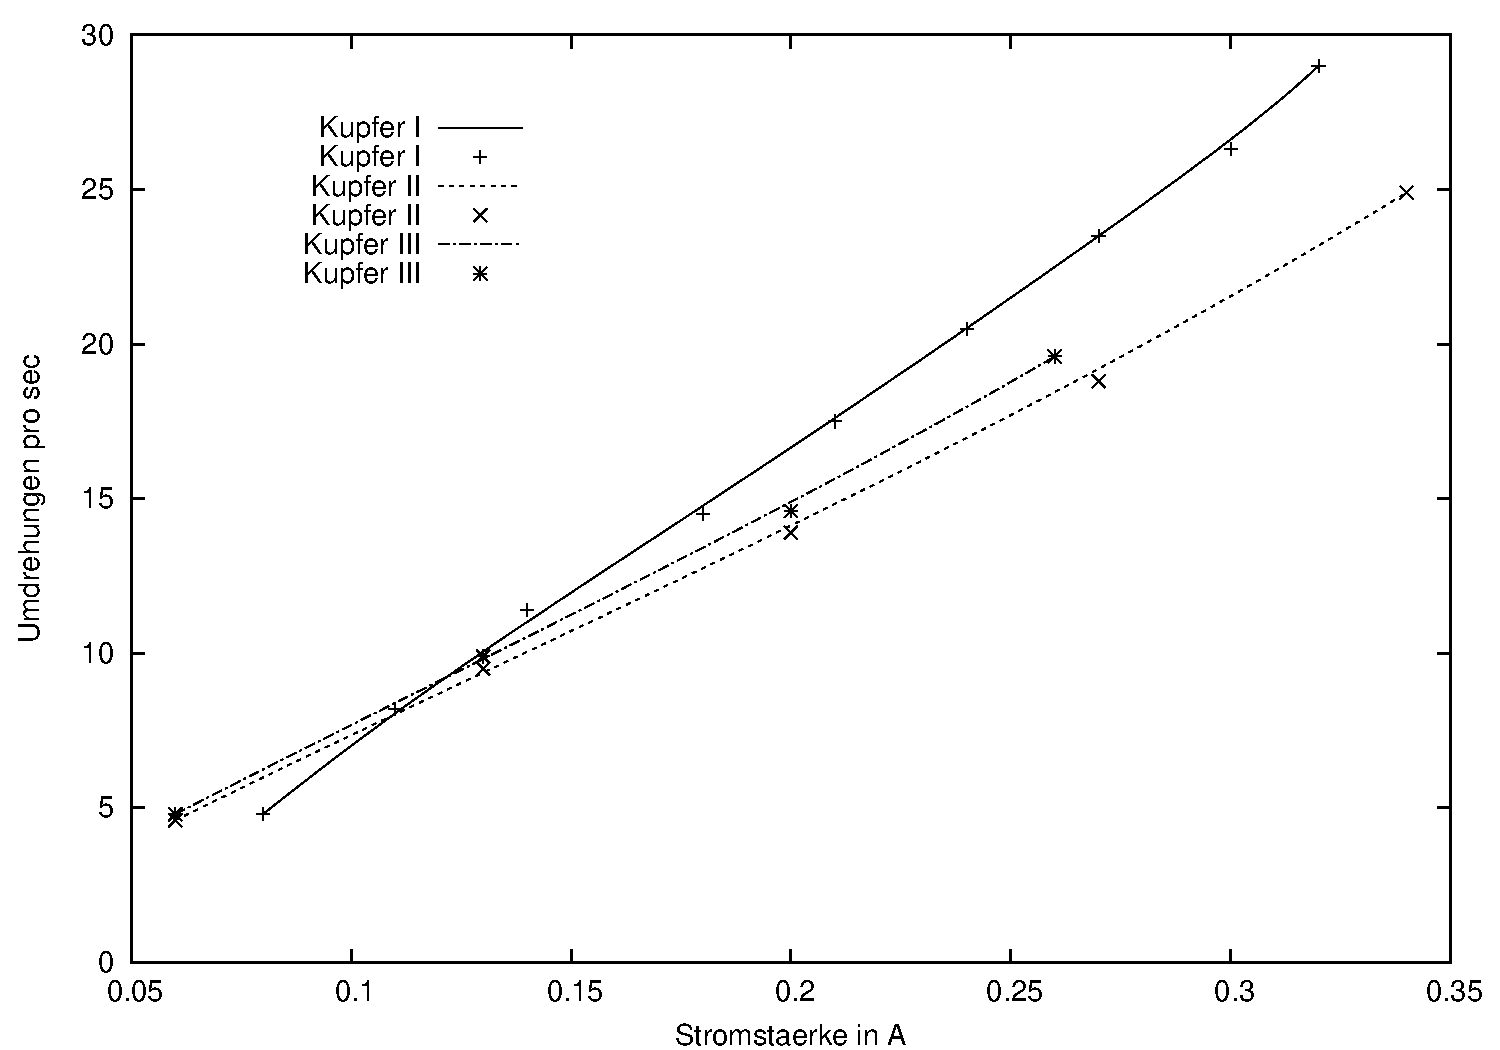
\includegraphics[width=0.95\textwidth]{praktika/mat_praktika/b2}
	\caption{Ergebnisse der Messung des Versuches aus Aufgabe \ref{wistrobre} mit einer Kupferscheibe. In dem Schaubild sind die Daten von drei verschiedenen Messungen enthalten -- Kupfer I bis III --, jeweils mit Datenpunkten und einer Ausgleichskurve.}
	\label{abbkup1a}
\end{figure}


\begin{figure}[htb]
	\centering
		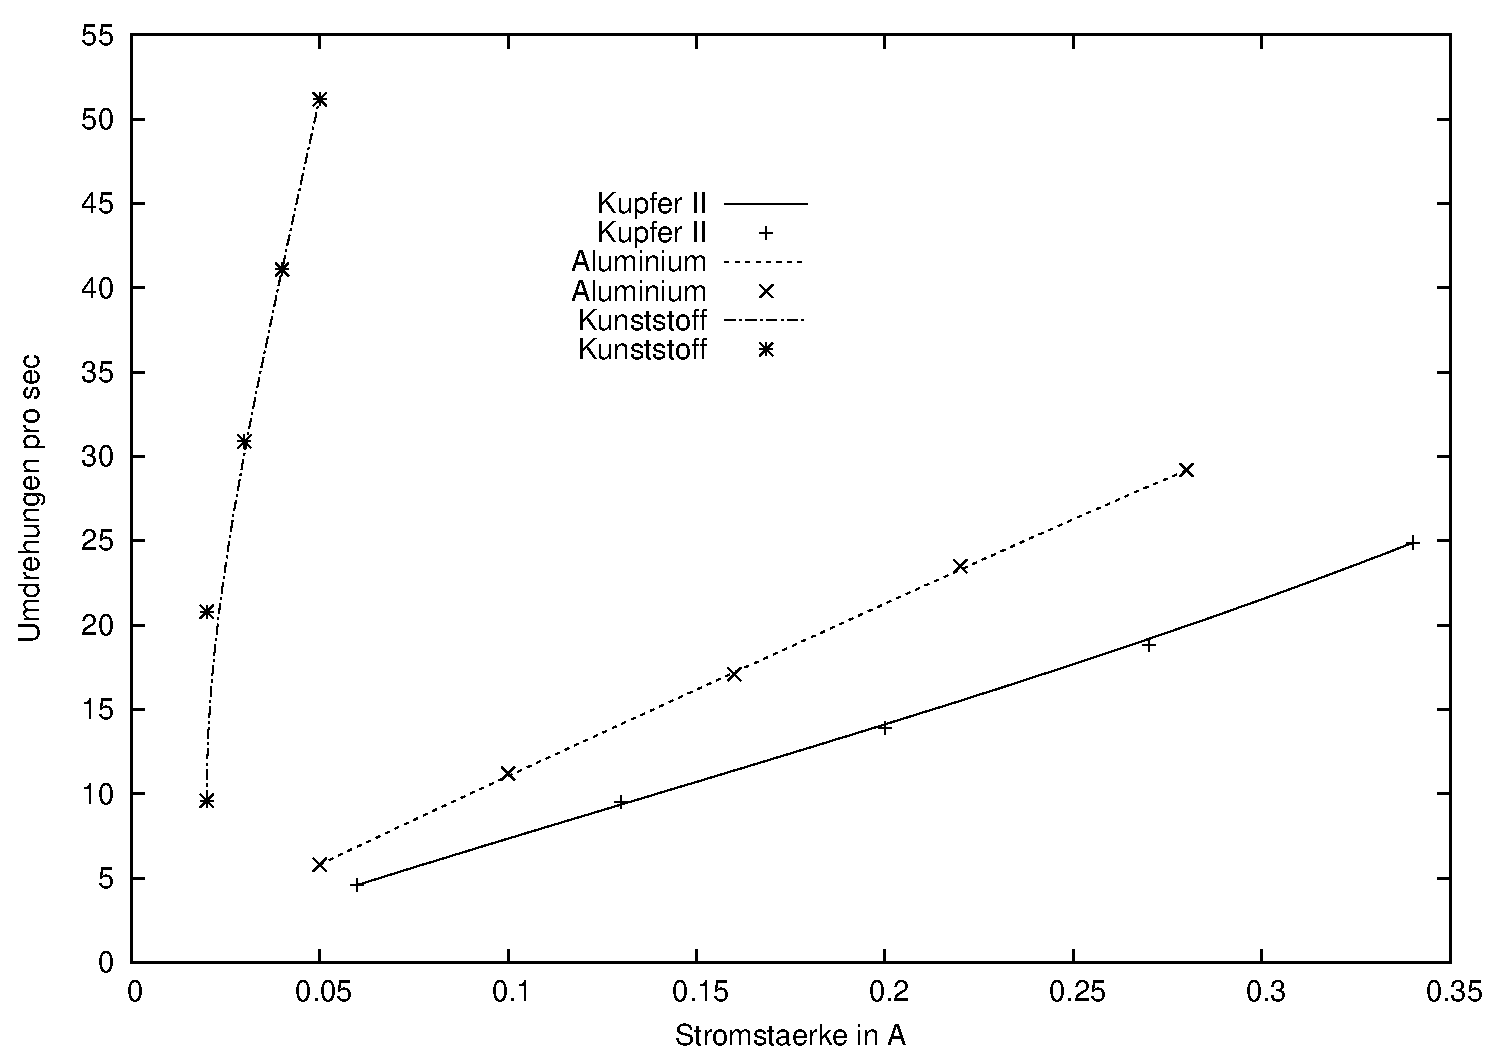
\includegraphics[width=0.95\textwidth]{praktika/mat_praktika/p1db1}
	\caption{Ergebnisse der Messung verschiedener Materealien des Versuches aus Aufgabe \ref{wistrobre} mit Ausgleichskurven.}
\label{verschmat}
\end{figure}


\begin{figure}[htb]
	\centering
		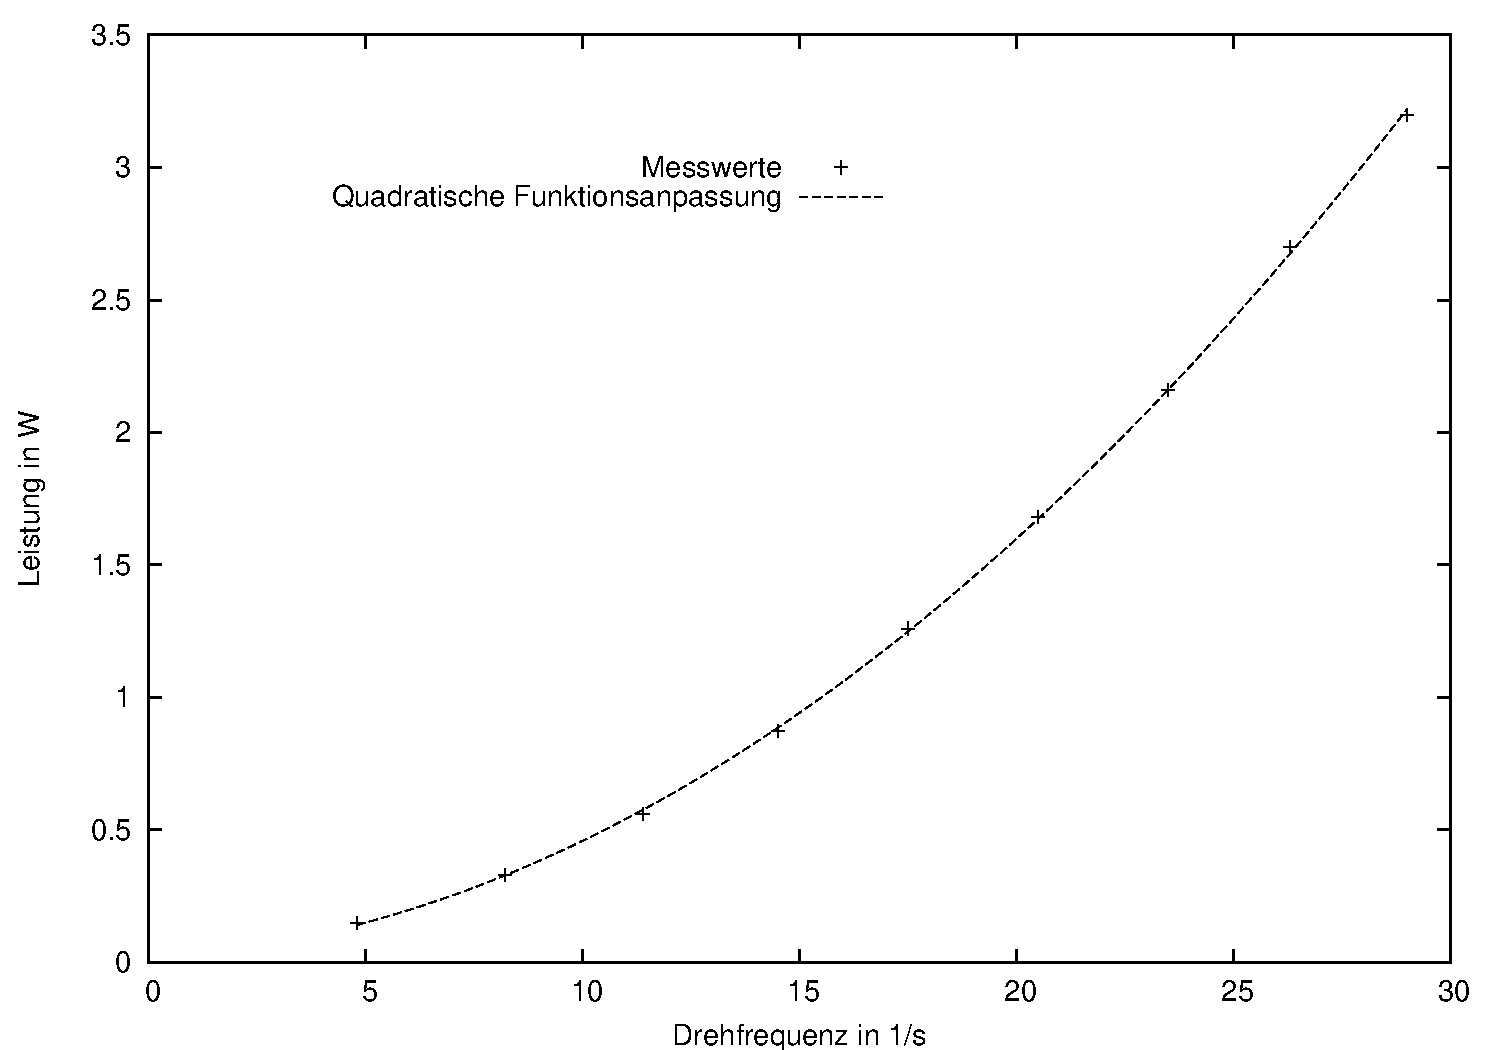
\includegraphics[width=0.95\textwidth]{praktika/mat_praktika/c}
	\caption{Ergebnisse der Messung Kupfer I des Versuches aus Aufgabe \ref{wistrobre} mit einer Kupferscheibe - mit quadratischer Regression}
	\label{abbkup1b}
\end{figure}


\begin{figure}[htb]
	\centering
		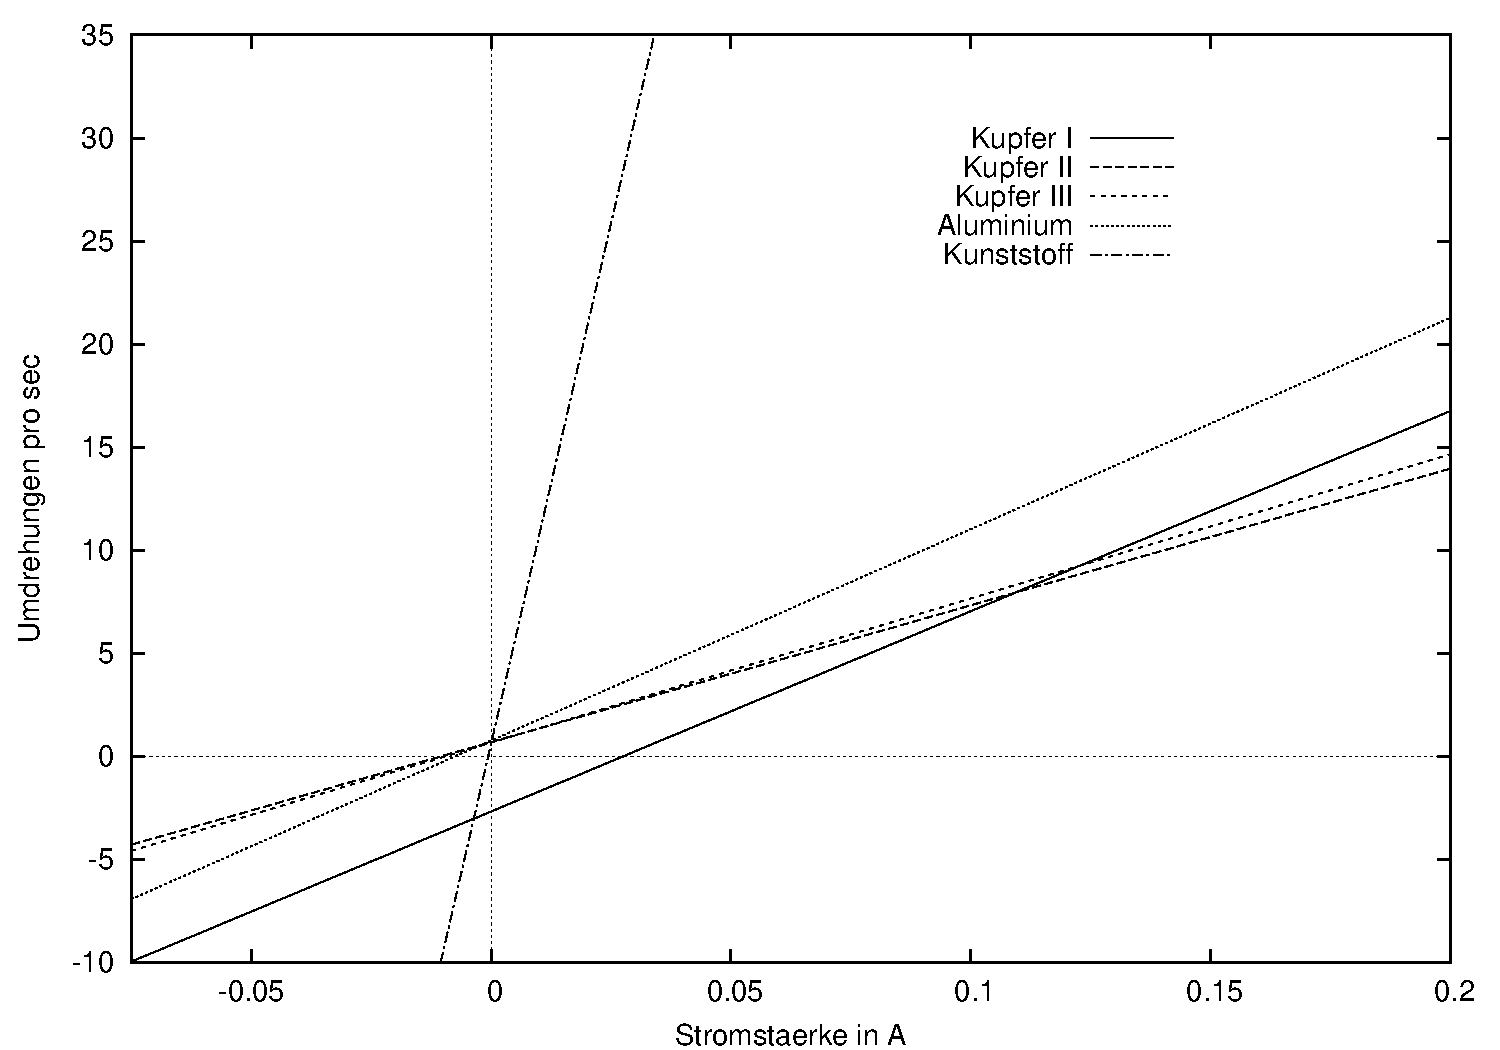
\includegraphics[width=0.9\textwidth]{praktika/mat_praktika/sa1}
	\caption{Die Ausgleichsgeraden aller Messungen zu Aufgabe \ref{wistrobre} in einem Schaubild eingetragen.}
	\label{ausglger}
\end{figure}





		\subsubsection*{Auswertung:}
In Abbildung \ref{abbkup1a} auf Seite \pageref{abbkup1a} ist die Drehfrequenz in Abhängigkeit zur Stromstärke aufgetragen. Es wurde eine Ausgleichsgerade eingetragen, die mit dem Messwerten äußerst gut übereinstimmt. Es liegt also nahe, dass Drehfrequenz und Stromstärke zueinander proportional sind. Es gilt also:
\begin{equation}
f \sim I
\label{eqsimfi}
\end{equation}
In Abbildung \ref{abbkup1b} auf Seite \pageref{abbkup1b} sind dann Leistung und Drehfrequenz gegeneinander aufgetragen. Dabei wird deutlich, dass die zur Drehung benötigte Leistung bei steigenden Drehfrequenzen quadratisch ansteigt. Es gilt also: 
\begin{equation}
P \sim f^2
\label{eqsimfp}
\end{equation}
Verbindet man \ref{eqsimfi} und \ref{eqsimfp}, so erhält man
\begin{equation}
P \sim I^2
\end{equation}
Das ist aber einfach erklärbar\footnote{Da im Motor der Strom durch Spulen fließt - also gewickeltem Draht - kann man nährungsweise davon ausgehen, dass es sich hierbei um einen \textsc{Ohm}'schen Widerstand handelt. Da der Motor mit Gleichstrom betrieben wird, sind Induktionsvorgänge vernachlässigbar.}, da ja 
\begin{equation}
P = I \cdot U ~~  \textnormal{und} ~~ U = I \cdot R ~~ \textnormal{und somit} ~~ P = I^2 \cdot R
\label{eq:ohmges}
\end{equation}
Aus Abbildung \ref{ausglger} auf Seite \pageref{ausglger} ist darüber hinaus ersichtlich, dass die Ausgleichsgeraden Ursprungsgeraden sind - nur eine widersetzt sich diesem Trend. Es könnte nun einerseits sein, dass hier bei besonders niedriger Umdrehungszahl die Reibung äußerst groß ist und die Kurve deshalb so nach unten \textit{absackt}. Wahrscheinlicher ist jedoch, dass mit den Messgeräten etwas nicht stimmt (da die Werte auf eine dermaßen exakten Linie liegen).

Daraus, dass Kurve des Kunststoffes wesentlich steiler ist, kann man ablesen, dass er für die selbe Drehfrequenz weniger Energie braucht. Dass dies auf das geringere Gewicht der Scheibe zurückzufürhen ist, ist unwahrscheinlich. Da eine Messung über 10 sec dauert, hatte der Motor -- wenn er eine schwerere und damit trägere Kupferscheibe antreibt -- genug Zeit, auch mit geringerer Beschleunigung seine maximale Geschwindigkeit zu erreichen. Es ist also davon auszugehen, dass die gemessenen Drehfrequenzen maximal für die Leistung des Motors ist und dabei nicht von der trägen Masse der Scheiben abhängt. 

Viel wahrscheinlicher ist, dass die Kupfer- und Aluminiumscheiben von der Wirbelstrombremse beeinflusst werden -- im Gegensatz zur Plastikscheibe. Der Motor muss somit, wenn er eine Kupferscheibe antreibt, immer gegen die bremsende Kraft der Wirbelstrombremse antreiben.

\clearpage
		\section{Strom- und Spannungsverlauf bei Selbstinduktion}
		\label{seind}
		
		\subsubsection*{Versuchsbeschreibung:}
Es wird ein Stromkreis gemäß Abbildung \ref{schzk} auf Seite \pageref{schzk} aufgebaut. Wenn der Schalter \(S_1\) geschlossen ist, so fließt Strom parallel - einerseits durch die Spule und \(R_2\), andererseits durch \(R_1\). Wird der Schalter \(S_1\) geöffnet, so fließt ein Induktionsstrom dem Verlauf der gestrichelten Pfeile nach, also in Reihe durch \(R_1\), \(R_2\) und die Spule. 

\begin{figure}[hp]
\centering
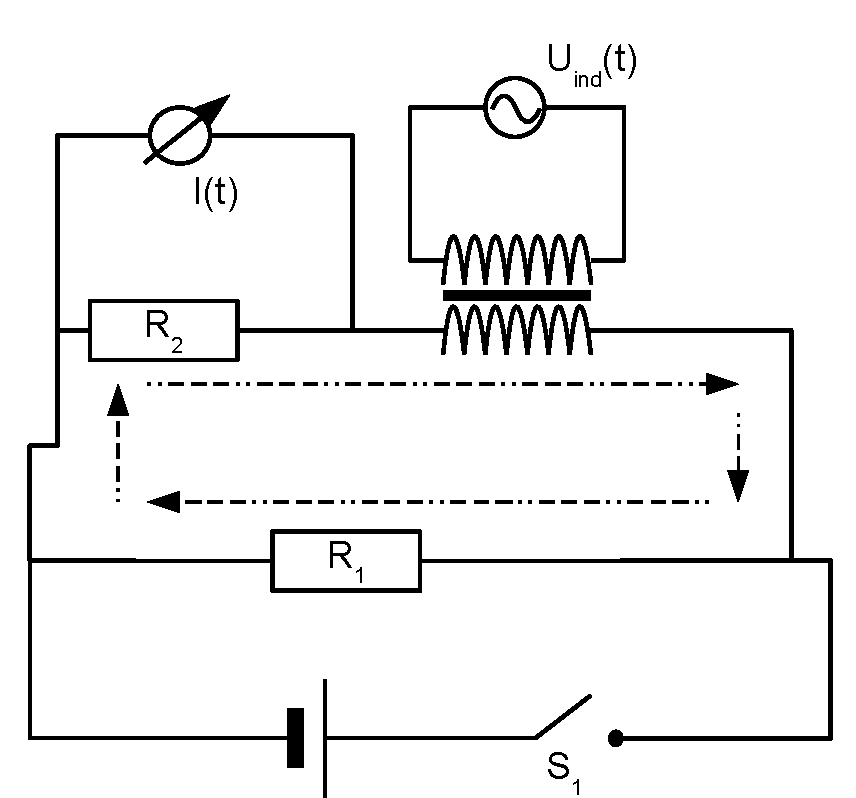
\includegraphics[width=0.3\textwidth]{praktika/mat_praktika/sz1}
\caption{Schaltdkizze zum Versuchsaufbau von Aufgabe \ref{seind}: \(R_1\) und \(R_2\) haben jeweils \(R_n = 220 \Omega\), die beiden Spulen haben jeweils \(n = 800\) Windungen, die Spannungsquelle liefert \(U_0 = 10V\) und der Schalter \(S_1\) ist ein \textit{Doppelreedrelais}, das mit der Frequenz \(f = 50 Hz\) umschaltet.}
\label{schzk}
\end{figure}

		

An \(R_2\) wird die Spannung gemessen. Da es sich bei \(R_2\) um einen Ohmschen Widerstand handelt, ist \(U(t) \sim I(t)\) (\(\rightarrow\) Gleichung \ref{eq:ohmges}). Deshalb ist es möglich, an \(R_2\) die Stromstärke \(I(t)\) abzulesen, da sie ja zu der eigentlich abgelesenen Spannung proportional ist.

An die zweite Spule, die mit der ersten durch einen gemeinsamen Eisenkern vebunden ist, wird ein Oszilloskop angeschlossen. Wird in der ersten Spule eine Induktionsspannung \(U_{ind}(t)\) induziert, so ist dazu ein sich änderndes Magnetfeld \(\dot{B} \neq 0\) nötig. Dieses sich ändernde Magnetfeld hat über den gemeinsamen Eisenkern auch in der zweiten Spule Auswirkungen, nämlich wird dort gemäß \(U_{ind} = n \cdot A \cdot \dot{B}\) die selbe Induktionsspannung wie in der ersten Spule induziert.

Somit kann man an \(R_2\) und der zweiten Spule \(I(t)\) bzw. \(U_{ind}(t)\) bestimmen.


		\subsubsection*{Beobachtungen:}
In Abbildung \ref{oszbu} auf Seite \pageref{oszbu} ist der Verlauf der Induktionsspannung dargestellt. In Abbildung \ref{oszbi} ist die Spannung dargestellt, die am Widerstand \(R_2\) abfällt. Vergleicht man die beiden Spannungsverläufe miteinander, so fällt auf, dass die Induktionsspannung	genau dann einen extremen \textit{Peak} nach oben macht, wenn der Strom gerade seinen Höchstpunkt erreicht hat und gerade am Absinken ist. Wenn der Strom gerade wieder ansteigt, so ist die Induktionsspannung stark negativ.


		\subsubsection*{Auswertung:}
Diese Phänomene sind duch \textit{Induktion} erklärbar. Wenn nämlich der Strom eingeschaltet wird, also in Schaubild \ref{oszbi} die Funktion sich gerade von der Zeitachse entfernt, ist die Änderung des Stromes \(\dot{I}(t)\) äußerst groß, da sich die Spannung ja von "`überhaupt kein Wert"' auf "`einen positiven Wert"' ändert. Nach 
\begin{equation}
	U_{ind}(t_n) = - L \cdot \dot{I}(t_n)
	 \label{lenz}
\end{equation}
ist die Induktionsspannung hier also stark negativ. Mit dem \textsc{Lenz}'schen Gesetz in Einklang ist diese Induktionsspannung also ihrer Ursache entgegengesetzt und "`\textit{fängt}"' die Veränderung der Stromstärke ab. Der Stromverlauf ist deshalb an dieser Stelle auch kurvenförmig. Ohne die entgegengerichtete Induktionsspannung hätte der Strom sein Maximum praktisch sofort erreicht. So nährt er sich seinem Maximum nur asymptotisch an.

Je mehr Zeit innerhalb einer halben Periode verstreicht, desto näher kommt der ausgebremste Strom seinem Maximum, aber immernoch ist eine gegenläufige Spannung da, die ihn dezimiert. Da er konsequent dezimiert wird, wird \(\dot{I}(t_N)\) auch kleiner, da ja ständig die wachstumsschwächende Induktionsspannung auf den Strom einwirkt.

Wenn der Strom dann wieder abgeschaltet wird, also von seinem Maximum abfällt (vgl Abbildung \ref{oszbi}), ist in Schaubild \ref{oszbu} ein noch größerer Peak entstanden, dier diesmal nach oben zeigt, also auch eine große positive Spannung hinweist. \(\dot{I}(t_n)\) ist an dieser Stelle stark negativ, weil der Strom sich von einem nahezu konstannten Wert "`\textit{erstmalig}"' abbewegt. Nach Gleichung \ref{lenz} sorgt diese Spannung nun dafür, dass der Stromstärkenabfall abgefangen wird, also nicht so drastisch aussieht.


\begin{figure}[h]
\centering
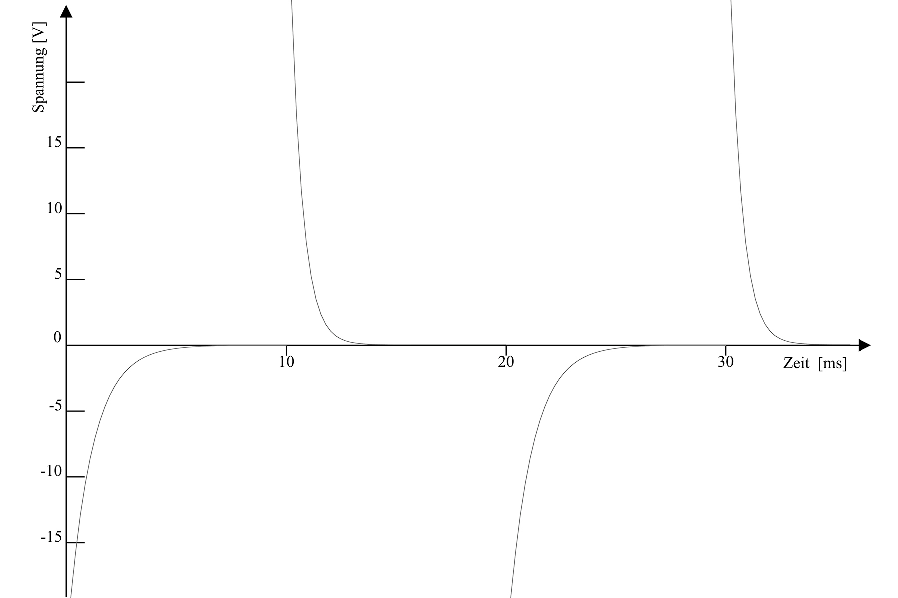
\includegraphics[width=0.85\textwidth]{praktika/mat_praktika/f1c}
\caption{Im Oszilloskop sieht der Spannungsverlauf von \(U_{ind}(t)\) so aus.}
\label{oszbu}
\end{figure}

\begin{figure}[h]
\centering
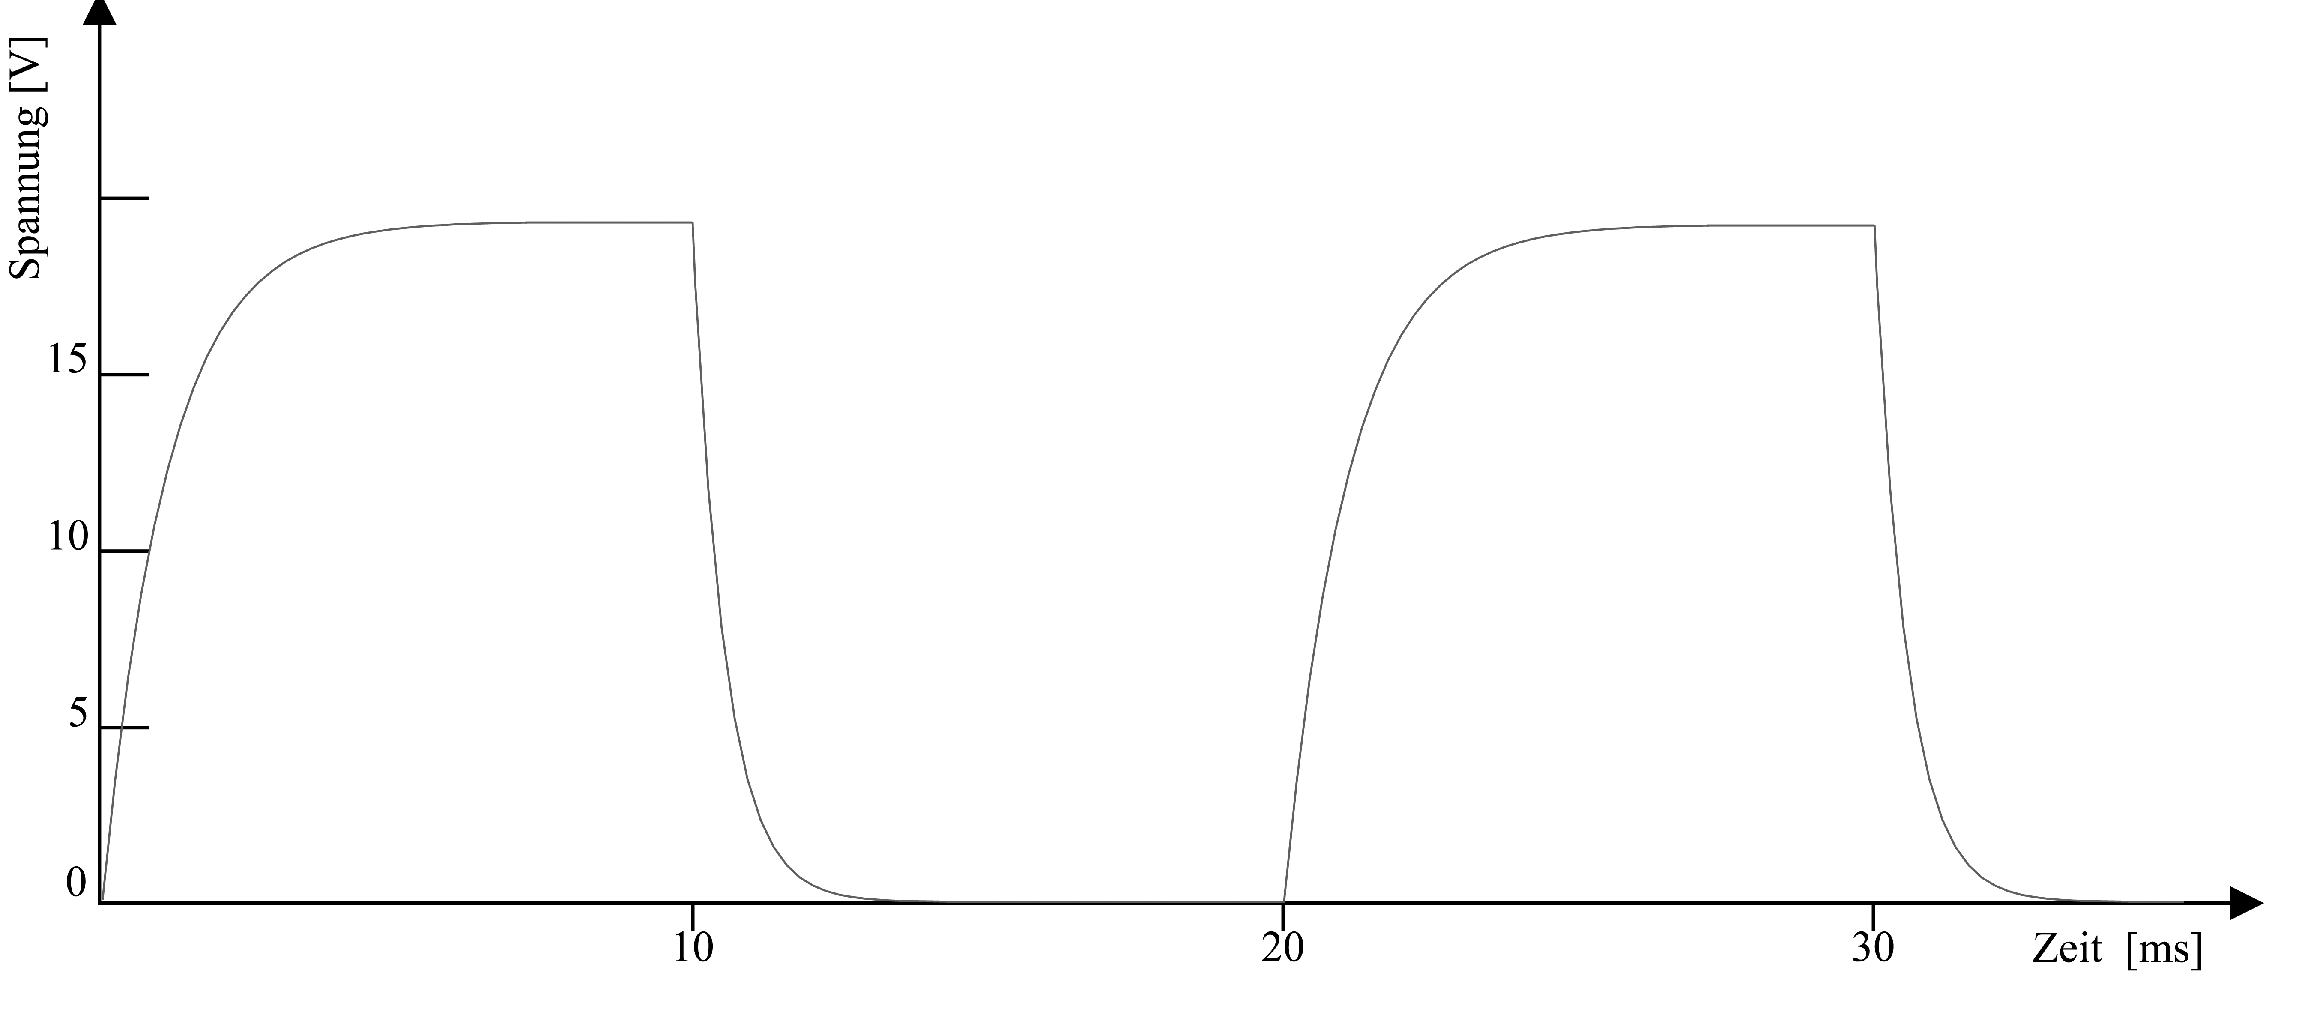
\includegraphics[width=0.85\textwidth]{praktika/mat_praktika/g1a}
\caption{Der Spannungsverlauf von \(U_{R_{2}}(t)\) dient zur bestimmung der Stromstäkre \(I(t)\)}
\label{oszbi}
\end{figure}

		





%\end{document}


\chapter{Versuche zur Schallgeschwindigkeit}
% \documentclass[a4paper]{article}
% \usepackage[ngerman]{babel}
% \usepackage[utf8]{inputenc}
% \usepackage[top=2.5cm,bottom=1.75cm,right=2cm,left=2.3cm]{geometry}
% \usepackage{wrapfig}
% \usepackage{floatflt}
% \usepackage{graphicx}
% \usepackage{subfigure}
% \usepackage[colorlinks=true,linkcolor=black,bookmarksnumbered=true,breaklinks=true,pdfstartview=FitH]{hyperref}
% 
% \title{\textbf{Praktikum 8} \\ ~ \\Schallgeschwindigkeit in Luft und Messing}
% 
% \author{Michael Kopp}
% 
% \date{17. Juli 2007}
% 
% \begin{document}
% 
% \maketitle


		\section{Versuch}



In ein Glasrohr werden feine Korkspäne gegeben und gleichmäßig verteilt. Dann sorgt man dafür, dass eine Schallwelle in das Rohr gelangt. Dort wird sie an den Rohrenden reflektiert. Um die Art der Reflexion zu beeinflussen, kann man eine der Öffnungen oder beide verschließen. Um die Länge des Rohres, in dem die Schallwellen schwingen können, zu beeinflussen, kann man einen der beiden Stopfen weiter nach innen oder außen bewegen.


\begin{figure}[h]
	\centering
	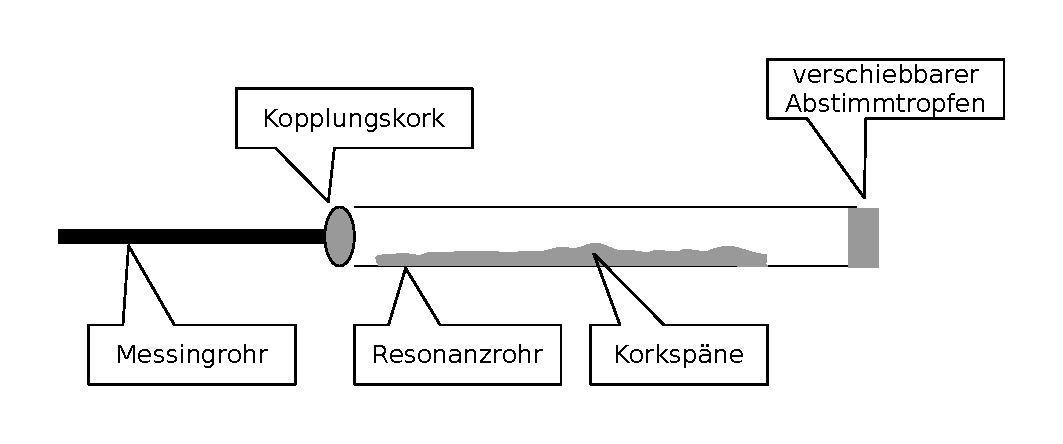
\includegraphics[width=0.8\textwidth]{praktika/mat_praktika/aufbau}
	\caption{Skizze des Versuchsaufbaus - sowohl das Messingrohr mit Kopplungskork als auch der Abstimmstopfen sind entfernbar.}
\end{figure}
Die Schallwellen werden dabei erzeugt durch 
\begin{enumerate}
	\item eine Stimmgabel 
	\item ein Messingrohr, an dem mit einem feuchten Lappen gerieben wird (dessen Schallwellen werden über ein \textit{Kopplungskork} an einem Ende der Röhre an die Luft im Rohr abgegeben)
	\item einen Lautsprecher, der mit einem Sinusgenerator betrieben wird
\end{enumerate}

Die Idee dahinter ist, dass sich in dem Rohr eine \textit{Stehende Welle} bildet. Diese hat dann \textit{Bewegungsbäuche}. Diese liegen immer an der selben Stelle und können hier die Korkspäne bewegen. An diesen Stellen werden die Korkspäne deshalb bald verschwunden sein, weil die Schallwellen sie immer in Längsrichtung zum Rohr bewegen. Sie sammeln sich dann an Stellen, an denen die Luft sich nicht (oder wenig) bewegt. Diese Stellen werden als \textit{Geschwindigkeitsknoten} bezeichnet.




		\section{Schallgeschwindigkeit in Luft}
		\label{kap:c_luft}



Das Resonanzrohr wird an einem Ende mit dem Abstimmstopfen verschlossen, dann wird eine Stimmgabel angeschlagen. Sei wird vor das offene Ende gehalten und der Abstimmstopfen wird so lange in das Resonanzrohr hineingeschoben bzw. herausgezogen, bis die Korkspäne sich zu kleinen Hügelchen anordnen - bis sich also eine \textit{stehende Welle} gebildet hat.

Bei dem Versuch wurde dabei eine Stimmgabel verwendet, die laut Hersteller mit einer Frequenz von \(f = 1700 Hz\) schwingt. Die verwendete Resonanzrohrlänge beträgt dabei \(L = 0,43m\). Misst man den Abstand zwischen zwei Spitzen der kleinen Hügelchen, so sollte man eigentlich die Entfernung \(\frac{\lambda}{2}\) messen können. Im Versuch ergab sich somit eine Wellenlänge von \(\lambda = 0.215m\).

Mit diesen Werten lässt sich die Schallgeschwindigkeit in Luft berechnen:
\begin{equation}
	c = \frac{\lambda}{T} = \lambda \cdot f = 0.215m \cdot 1700\frac{1}{s} = 365,5 \frac{m}{s} \approx 366 \frac{m}{s}
	\label{c_luft}
\end{equation}
Der Literaturwert der Schallgeschwindigkeit beträgt \(c_{lit} = 343 \frac{m}{s}\), wir haben in unserem Fall also eine Abweichung von ca. \(6,56\%\). Das sieht eigentlich ganz gut aus - nur leider muss an den Werten etwas falsch sein. Da das Resonanzrohr an einer Seite geschlossen ist und an einer Seite offen, sollte sich eigentlich eine Stehende Welle bilden, die an der geschlossenen Seite einen Wellenknoten\footnote{Geschwindigkeitsknoten} und an der offenen Seite einen Wellenbauch\footnote{Geschwindigkeitsbauch} hat.

Für eine stehende Welle, die diese Bedingungen erfüllt, existiert die Formel 
\begin{equation}
	L = k \cdot \frac{\lambda_k}{4} ~~~~ k = (1; 3; 5 ...)
	\label{offenzu}
\end{equation}
Setzt man die gefundenen Werte für \(\lambda\) und \(L\) ein, so erhält man \(k = 8\) - und das sollte eigentlich nicht möglich sein. Es ist nichtsdestoweniger überraschend, wie präzise die Werte stimmen.\footnote{Auch bei anderen Gruppen kommt dieses eigentlich unsinnige Ergebnis heraus: bei einer Rohrlänge von \(L = 0,55m\), einer Frequenz von \(f = 1700Hz\) und einer gemessenen Wellenlänge von \(\lambda = 0,22m\) kommt exakt \(k = 10\) heraus.}

Eine mögliche Erklärung dafür könnte sein, dass die Stimmgabel zu nahe an die Öffnung gehalten wurde, und sich somit faktisch die Bedingung für zwei geschlossene Enden ergibt - dann hätte man \(k^* = 4\) und damit einen erlaubten Wert.


\subsection{Schaubilder}

Im Folgenden sind ein paar Schaubilder abgebildet, die sich auf die stehende Welle im Resonanzrohr beziehen. Es ist dabei ersichtlich, dass die Teilchen sich in Richtung des Rohres hin und her bewegen (siehe Abbildung \ref{s} auf Seite \pageref{s}) und dabei sich ein Druck an den Stellen aufbaut, an denen die Teilchen dicht nebeneinander liegen (siehe Abbildung \ref{p} auf Seite \pageref{p}). An der linken Seite - also Am Stopfen - bewegt sich das Teilchen nie (siehe Abbildung \ref{v} auf Seite \pageref{v}).

Wenn die Teilchen \textit{maximal ausgelenkt} sind (also jeweils im oberen Schaubild), bewegen sie sich kurzzeitig nicht, es besteht aber der größte Druck zwischen ihnen. Durchlaufen sie ihre \textit{Ruhelage} (jeweils im unteren Schaubild), so haben sie die maximale Geschwindigkeit, jedoch herrscht ein einheitlicher Normaldruck zwischen ihnen.

An den Stellen, an denen in Abbildung \ref{v_t0} die Funktion die x-Achse schneidet, herrscht nie Luftbewegung. Hier in der Nähe werden sich die Korkspäne sammeln, die von den Stellen ``weggeschubst'' werden, an denen die Funktion eben \emph{nicht} Null ist.




\begin{figure}
 	\centering

\subfigure[Hier sind sie bei der maximalen Auslenkung gezeigt (bspw. \(t = 0\))]{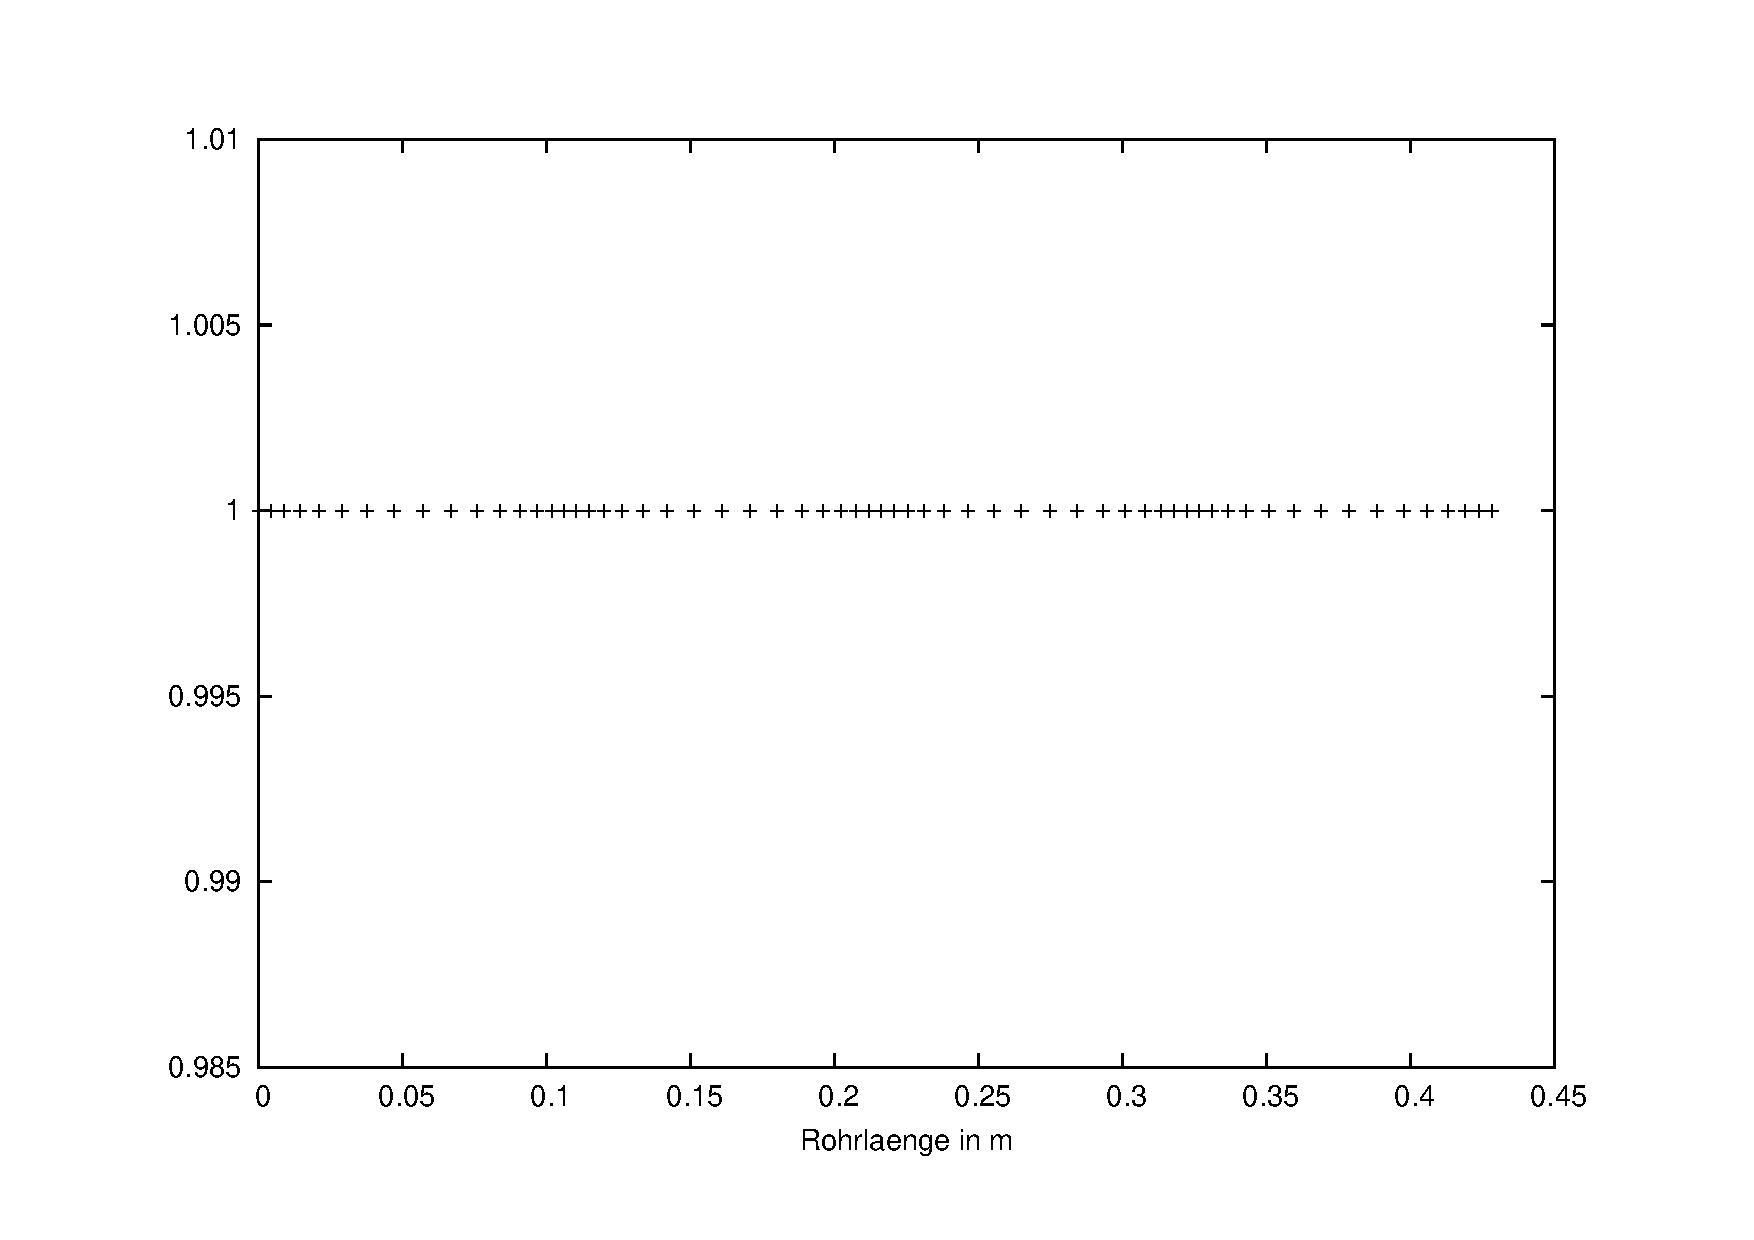
\includegraphics[width=0.9\textwidth]{praktika/mat_praktika/long01}\label{s_t0}}


\subfigure[Hier sind sie in Ruhelage gezeigt (bspw. \(t = \frac{T}{4}\))]{
	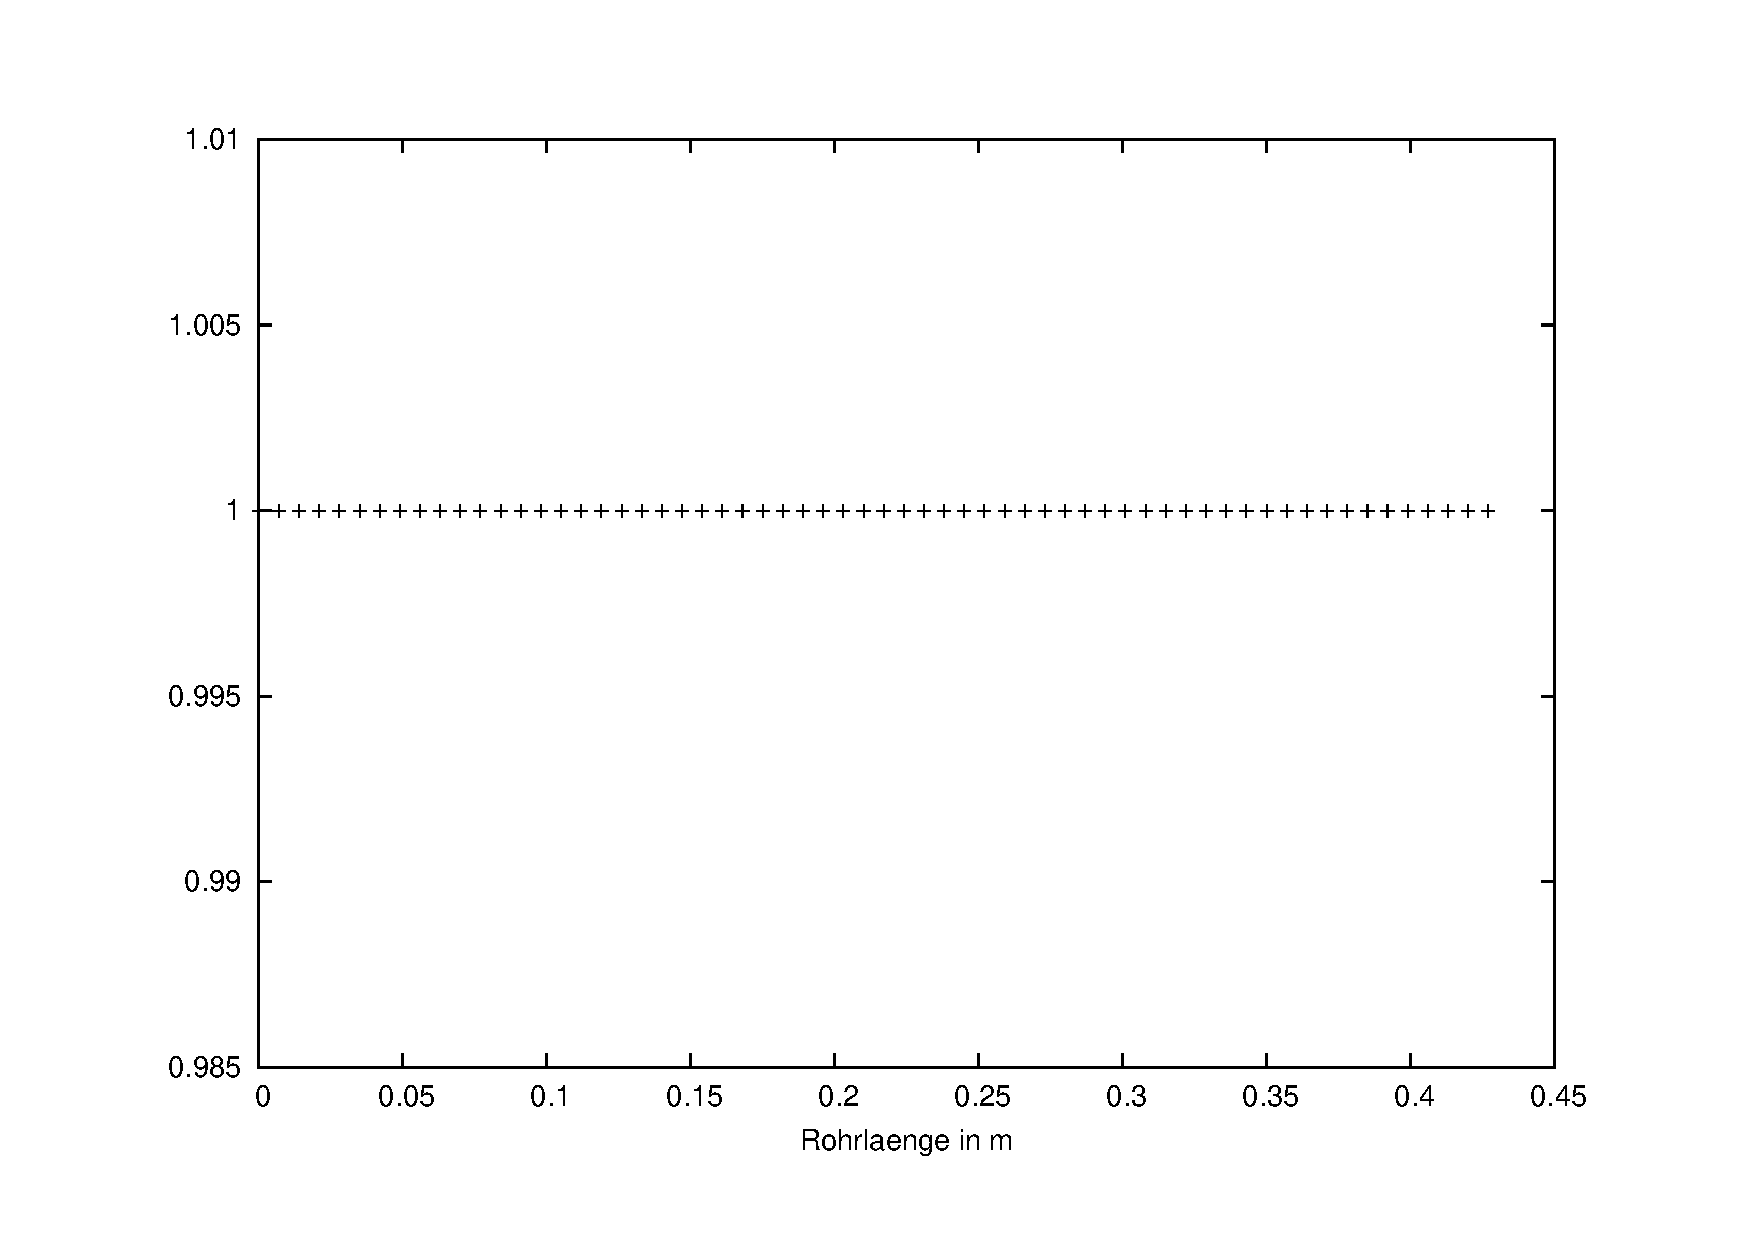
\includegraphics[width=0.9\textwidth]{praktika/mat_praktika/long02}\label{s_t1}}

\caption{In diesem Schaubild sind Luftteilchen eingezeichnet, die in der Ruhelage alle 7mm voneinander entfernt liegen würden. Bei \(x = 0\) kann man sich den Stopfen vorstellen.}
\label{s}
\end{figure}


\begin{figure}
	\centering
 	\subfigure[Die Teilchen bei maximaler Auslenkung (bspw. \(t = 0\))]{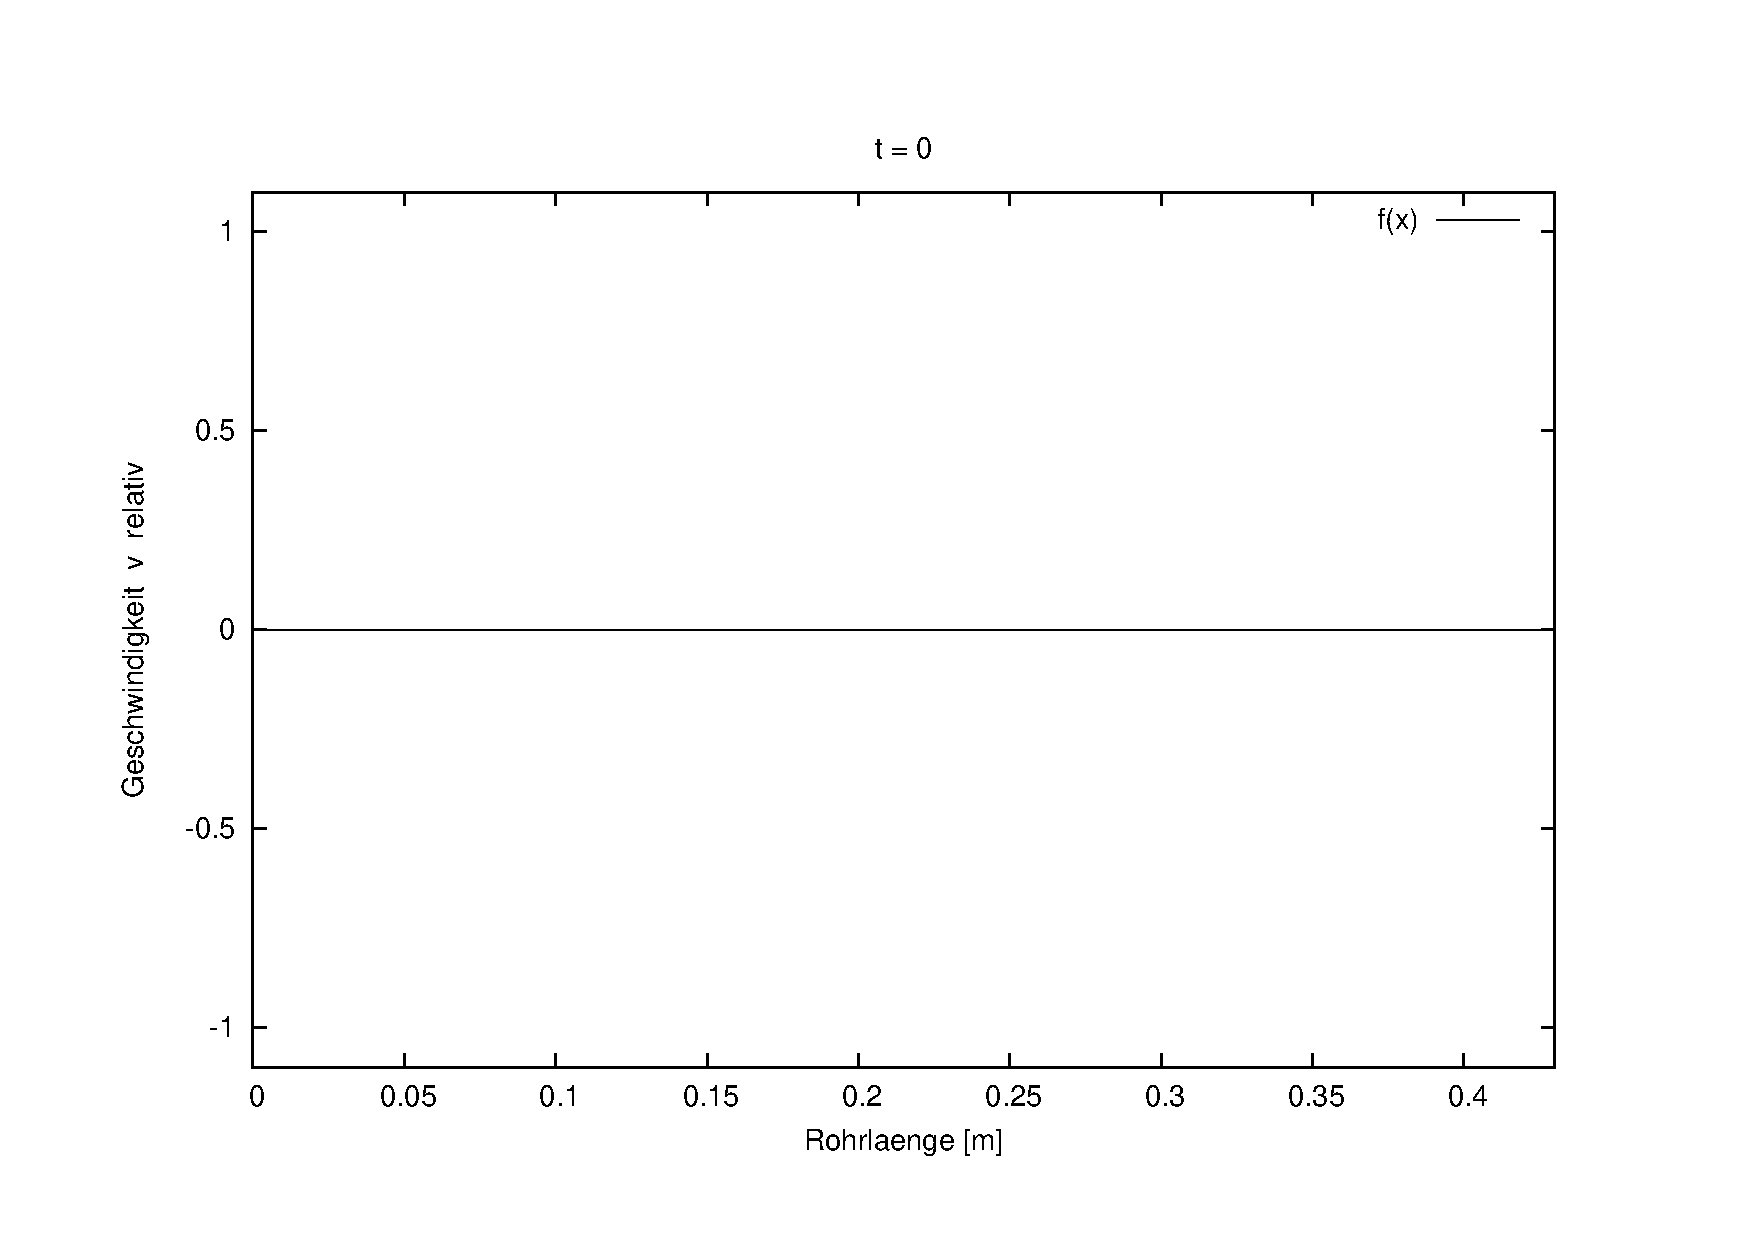
\includegraphics[width=0.9\textwidth]{praktika/mat_praktika/ges01}\label{v_t0}}

	\subfigure[Die Teilchen in Ruhelage (bspw. \(t = \frac{T}{4}\))]{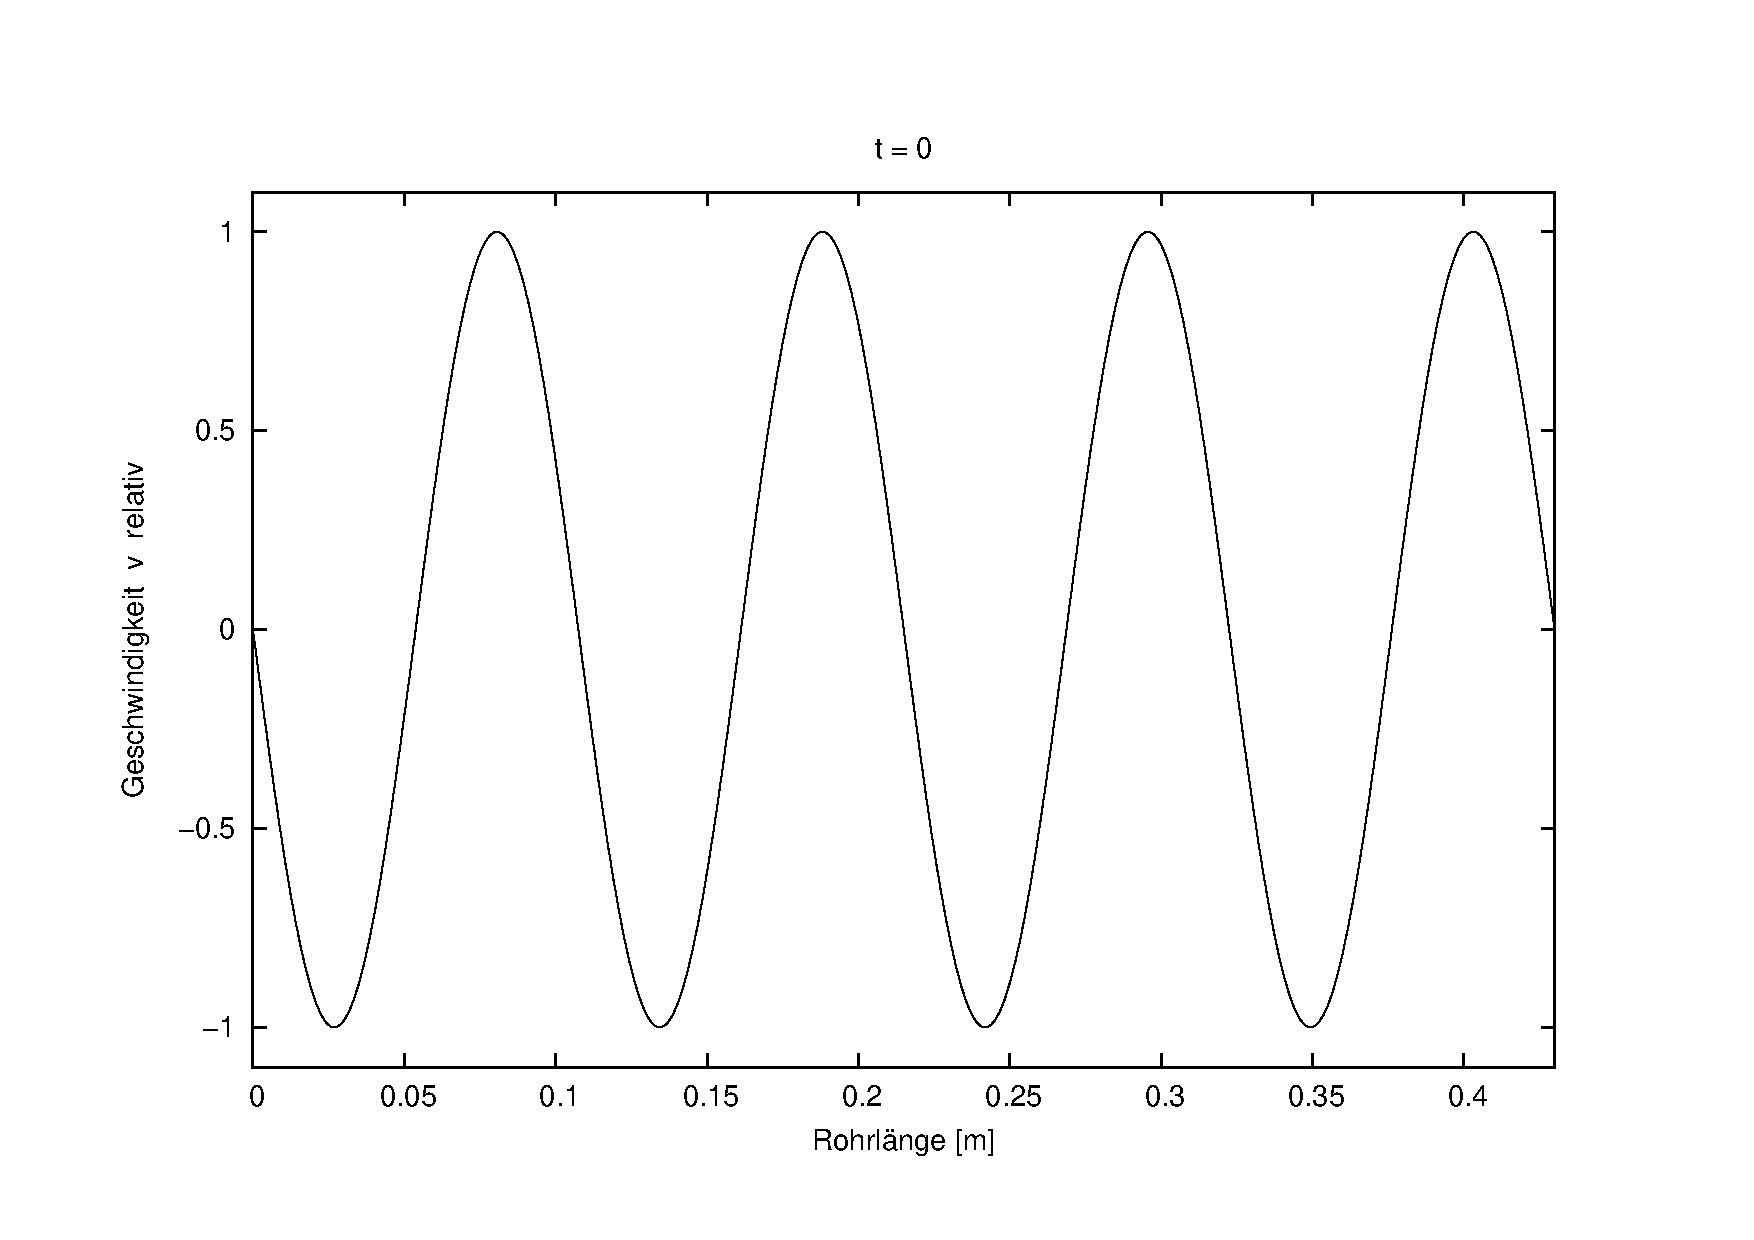
\includegraphics[width=0.9\textwidth]{praktika/mat_praktika/geschw02}\label{v_t1}}

	\caption{Hier sind die relativen Geschwindigkeiten der Luftteilchen eingetragen.}\label{v}
\end{figure}


\begin{figure}
	\centering
 	\subfigure[Die Teilchen bei maximaler Auslenkung (bspw. \(t = 0\))]{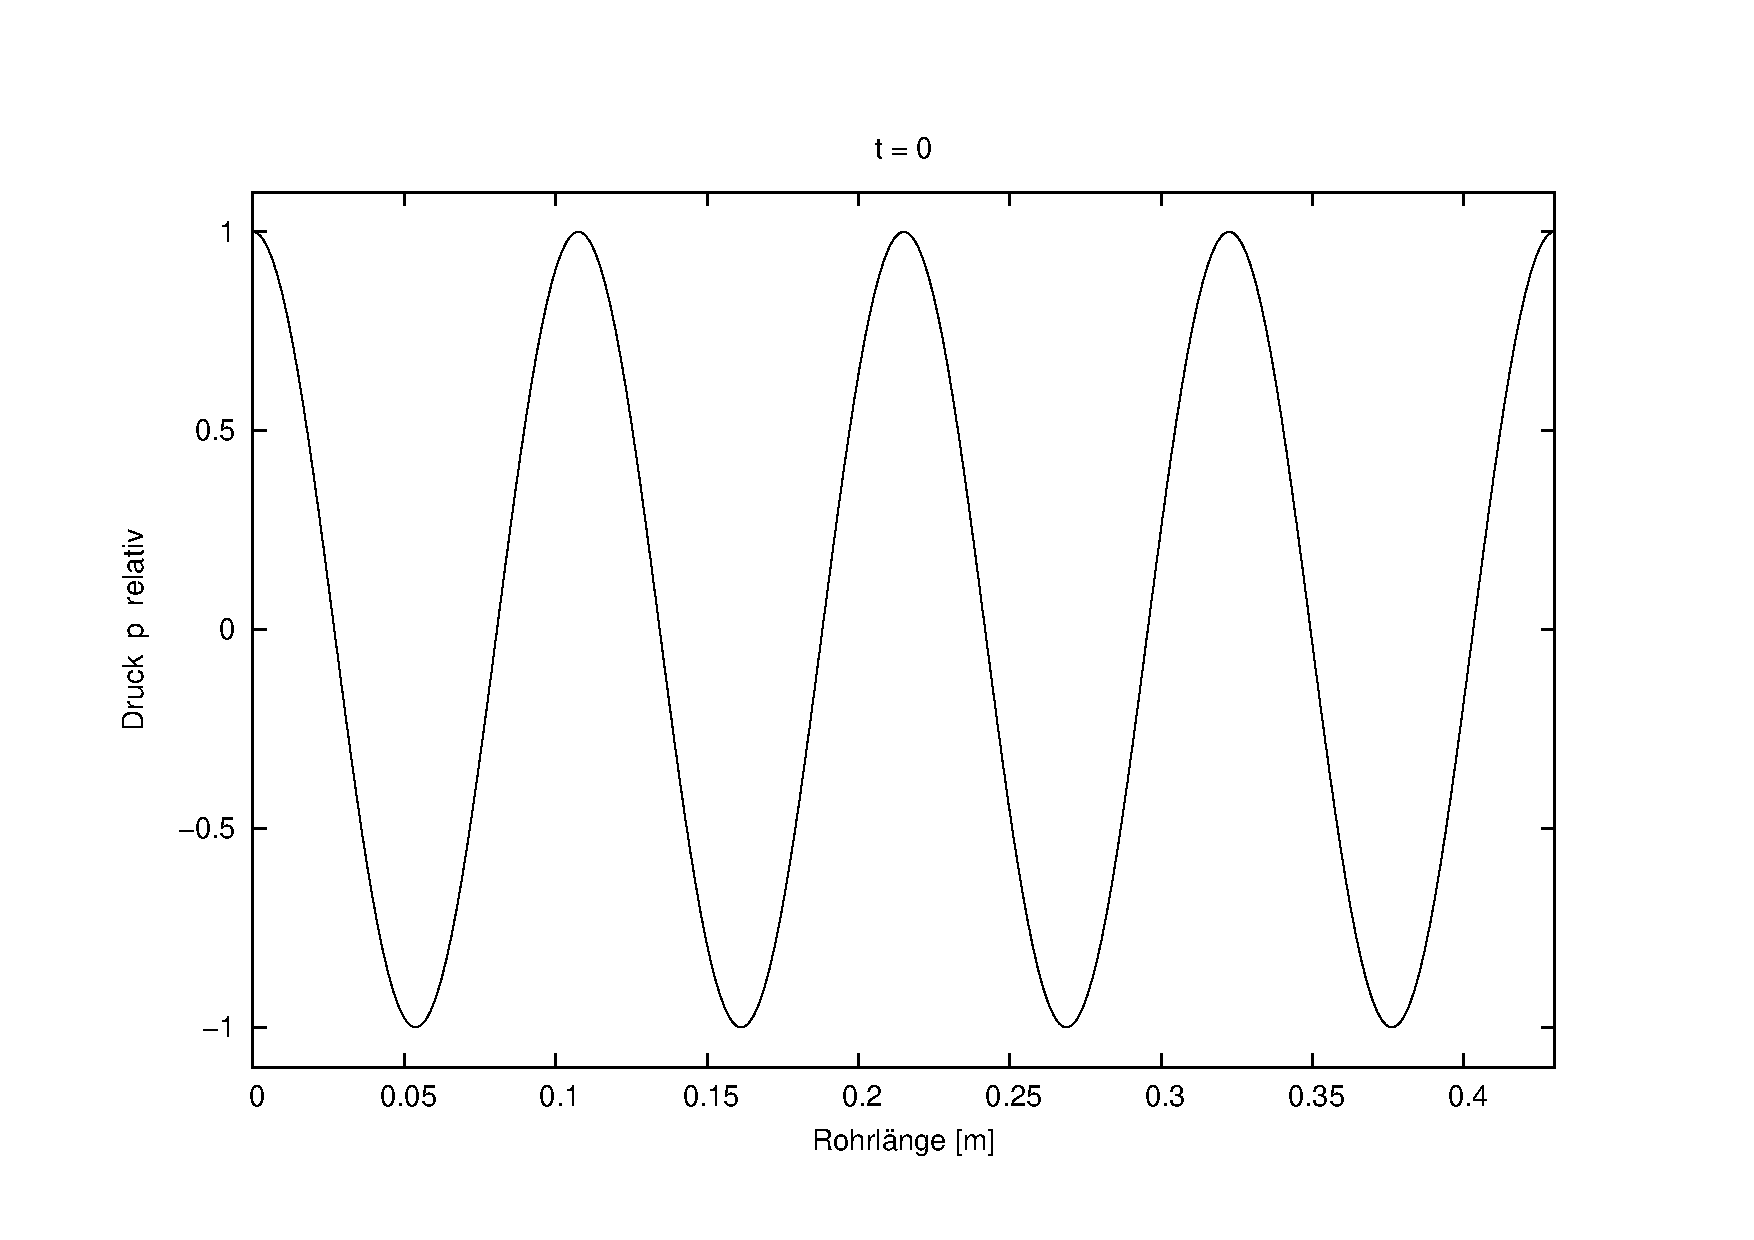
\includegraphics[width=0.9\textwidth]{praktika/mat_praktika/druck01}\label{p_t0}}

	\subfigure[Die Teilchen in Ruhelage (bspw. \(t = \frac{T}{4}\))]{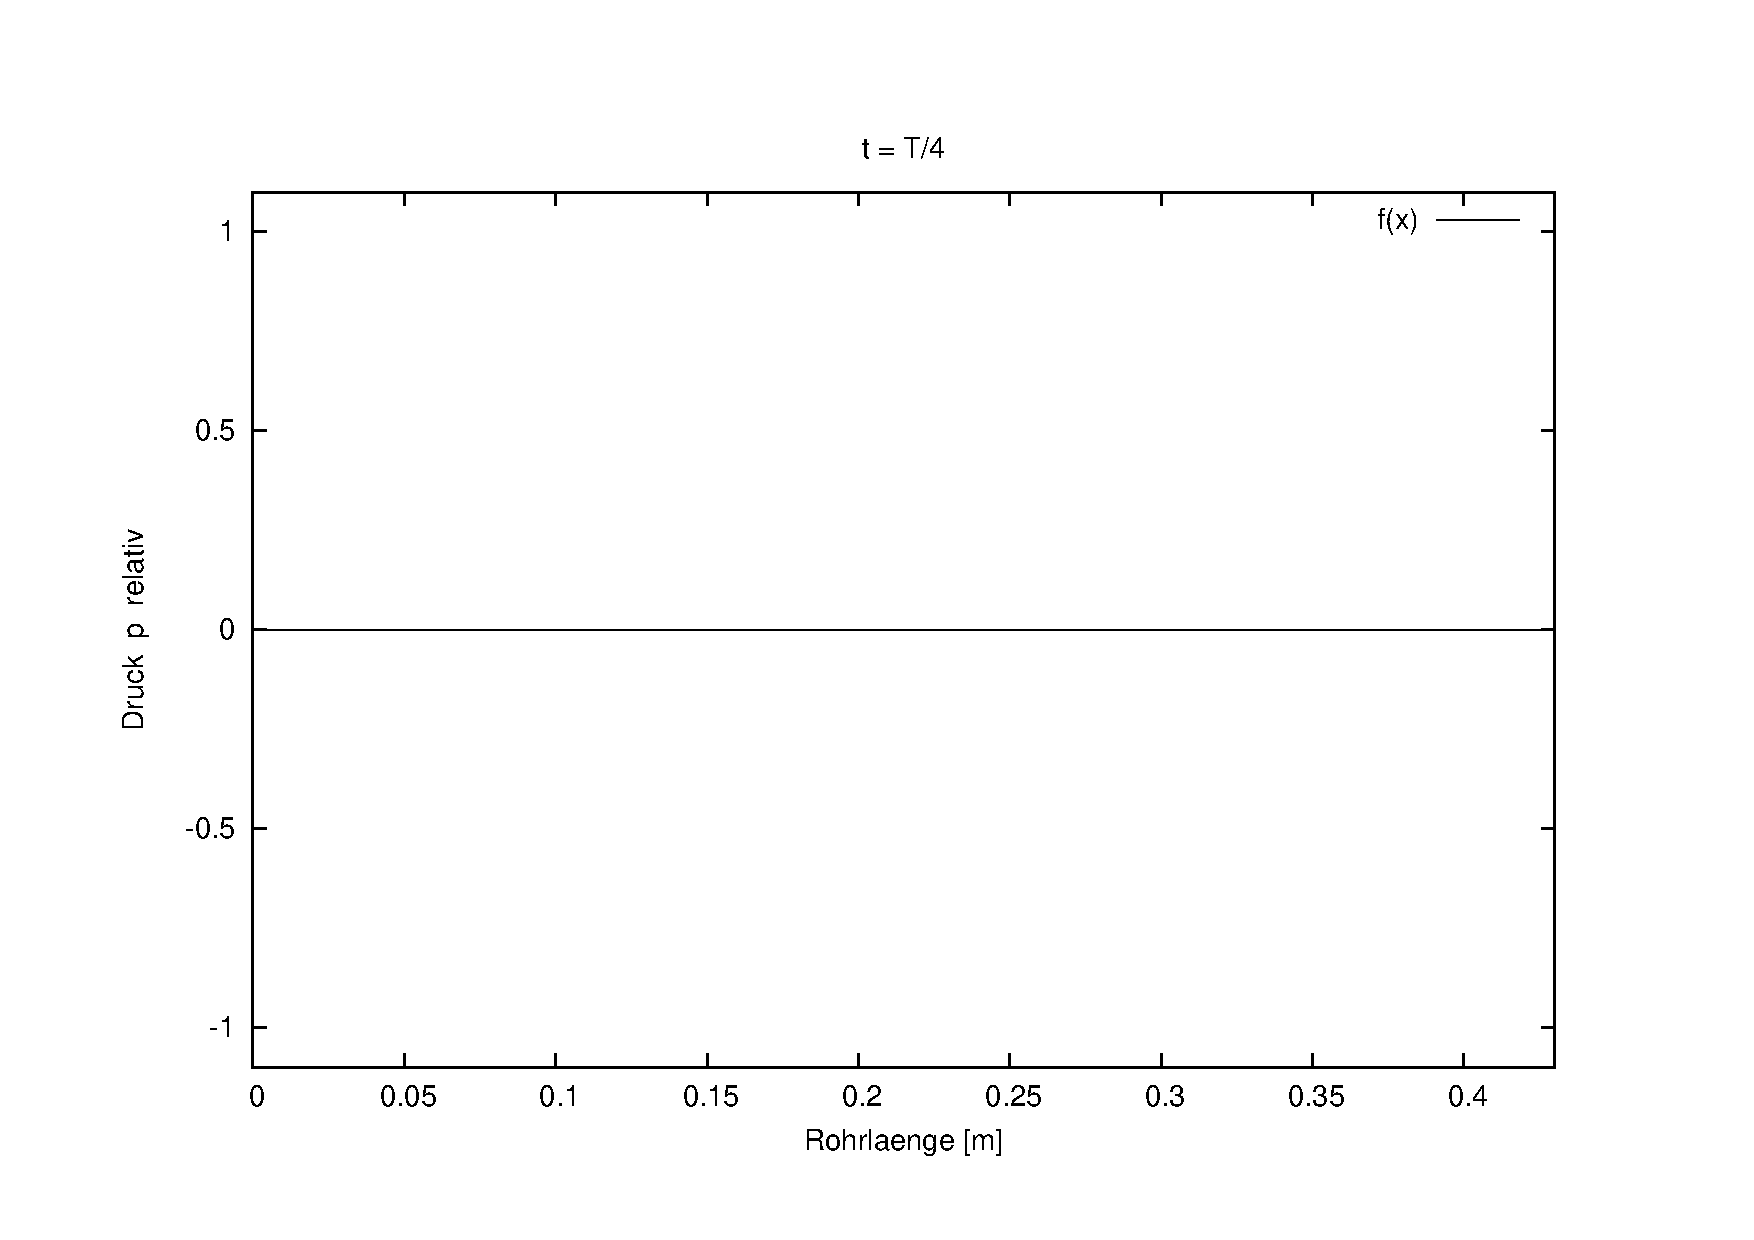
\includegraphics[width=0.9\textwidth]{praktika/mat_praktika/dru02}\label{p_t1}}

	\caption{Hier sind die relativen Drücke der Luft eingetragen.}\label{p}
\end{figure}


\clearpage



		\section{Schallgeschwindigkeit in Messing}

Nun wird auf das noch offene Ende des Resonanzrohres das Erregerrohr aus Messing aufgesetzt. Genau in der Mitte wird es eingespannt. An dieser Stelle ist also gewissermaßen ein Geschwindigkeitsknoten erzwungen. Die Enden des Stabes dagegen können (ziemlich\footnote{An der Stelle mit dem Kopplungskork zwar weniger, es handelt sich hier aber nicht um ein feste Ende, weil der Kork so ausgelegt ist, die Bewegung des Messingrohres weiterzuleiten - er darf sie also nicht bremsen.}) frei schwingen. 

Durch die Anregung des Rohres mit einem nassen Lappen dürften sich Transversalstörungen und sogar Transversalwellen bilden. Diese dürften dann an den Enden des Messingrohrs reflektiert werden\footnote{teilweise werden sie am Kopplungskork an die Luftsäule abgegeben}. Somit müsste sich im Messingrohr eine stehende Transversalwelle bilden. Durch die vorgegebenen Bedingungen\footnote{an den beiden freien Enden Schwingungsbäuche und in der Mitte ein Schwingungsknoten} kann das Rohr nur in bestimmten Frequenzen mit einer stehenden Welle schwingen - nämlich nur dann, wenn sich nach der entsprechenden Wellenlänge und der Formel
	\begin{equation}
 	L = k \cdot \frac{\lambda_k}{2}
	\label{2offen}
\end{equation}
\emph{ungerade} \(k\) ergeben\footnote{also \(k = (1;3;5;...)\)}. Das Rohr kann also in seiner Grundschwingung (1. Harmonische) schwingen, dann aber erst wieder in der 3. Harmonischen, aber nicht in der 2. Harmonischen (der \emph{Oberschwingung}).


Ist die Länge \(L_{mess}\) des Messingrohres bekannt, so kann man damit die Schallgeschwindigkeit in Messing berechnen. Hierzu versetzt man das Messingrohr in Schwingungen, bis sich eine harmonische Schwingung ergeben hat. Bei dieser zählt man dann die \textit{Wellenknoten} - diese Anzahl ergibt den Faktor \(k\). Die Frequenz \(f\), mit der das Messingrohr schwingt, muss man so herausfinden wie in Kapitel \ref{kap:c_luft}.

Schwingt das Messingrohr also, stellt man den Abstimmstopfen so ein, dass sich die Korkspähne im Rohr wieder zu Hügelchen anordnen. Zwischen diesen misst man dann die Abstände und damit \(\frac{\lambda}{2}\). Über die schon vorher errechnete Schallgeschwindigkeit in Luft \(c\) kann man so nach Formel \ref{c_luft} einfach die Frequenz bestimmen, mit der die Luftsäule schwingt. Sie ist genauso groß, wie die Frequenz, mit der das Messingrohr schwingt - in unserem Falle war \(\lambda = 0,1434m\), somit ergibt sich
	\begin{equation}
 f_{mess} = \frac{c}{\lambda} = \frac{365,5\frac{m}{s}}{0,1434m} = 2548,8 \frac{1}{s} \approx 2,55 kHz
\end{equation}
Über die Zusammenhänge aus Formel \ref{c_luft} und \ref{2offen} ergibt sich für die Schallgeschwindigkeit in Messing bei einem Messingrohr der Länge \(L_{mess} = 0.67m\), das mit einem einzigen Wellenknoten (\(k = 1\)) mit der Frequenz \(f_{mess} = 2548,8 Hz\) schwingt die Schallgeschwindigkeit
	\begin{equation}
 	c_{mess} = \frac{2 \cdot f_{mess} \cdot L_{mess}}{k} = 2 \cdot 2548,8 \frac{1}{s} \cdot 0,67m = 3415,4 \frac{m}{s}
	\label{causf}
\end{equation}
Diese Berechnung war sehr präzise - der Literaturwert liegt bei \(3400 \frac{m}{s}\), das ergibt eine Abweichung von \(0,45\%\).


~\\


Ironischerweise befindet sich der Kopplungskork dabei an einem Geschwindigkeits\emph{knoten}. Das ist aber leicht zu erklären, weil es sich bei dem Kork ja immer noch um ein festes Ende handelt, das bei einer stehenden Welle eben \emph{immer} einen Geschwindigkeitsknoten hervorruft. 

Gleichzeitig ist an der Stelle aber ein \emph{Druckbauch}. Das ist nun wieder leicht zu verstehen und auch bildhaft vorzustellen: Der Kopplungskork wandelt die Transversalwellen des Messingrohres in Longitudialwellen um. Dabei drückt er die direkt vor ihm liegende Luft abwechselnd zusammen (erzeugt also Überdruck), um dann wieder beim Zurückweichen einen Unterdruck zu erzeugen (der die Teilchen wieder auseinander zieht). Die Teilchen direkt am Kork werden dabei aber wenig bewegt; sie geben praktisch nur den Druck weiter.




		\section{Erregung mit Lautsprecher}


Nun werden beide Enden des Rohres frei gemacht und ein Lautsprecher wird vor eines der beiden offenen Enden positioniert. Er hat etwas Abstand zum Rohr, damit sich hier kein geschlossenenes Ende ergibt. Nun wird der Lautsprecher an einen Sinusgenerator angeschlossen und bei diesem wird die Frequenz so lange geändert, bis sich die bereits beobachteten Resonanzphenomäne einstellen - bis der Kork sich also wieder in Häufchen anordnet. Ist das geschehen, wird die Frequenz möglichst präzise gemessen - dazu verwendet man ein Mikrophon, das an ein Oszilloskop angeschlossen wird. Das Mikrophon kann man hinter dem zweiten offenen Ende des Rohes positionieren; auch wenn der Schall hier eigentlich in das Rohr zurück reflektiert wird, werden stets genügend Luftteilchen in der Umgebung mit angeregt, um den Schall aus dem Rohr hinauszutragen.

Diese Messung ergab eine Frequenz von \(f_{anr} = \frac{1}{0,0012s} \approx 833,3Hz\). Da de stehende Welle hier aufgrund der Bedingung zweier loser Enden zustande gekommen ist, kann man Formel \ref{2offen} heranziehen, wobei diesmal alle positiven, ganzzahligen \(k\) erreicht werden dürfen.\footnote{\(k = (1; 2; 3; ...)\)} Durch abzählen der \textit{Geschwindigkeitsbäuche} (also der Stellen, an denen \emph{kein} Kork liegt) erhält man den Faktor \(k\) - in unserem Falle ist \(k = 2\). Die Länge des Rohres beträgt \(L_{Rohr} = 0,43m\). Wir können hier die Umformung von Formel \ref{causf} verwenden\footnote{Die Formel aus den Bedingungen ``zwei offene Enden'' ist die selbe wie für die Bedingungen ``zwei geschlossene Enden''.}. Es ergibt sich für uns also:
\begin{equation}
 	c_{Luft} = \frac{2 \cdot f \cdot L_{Rohr}}{k} = \frac{2 \cdot 833,3\frac{1}{s} \cdot 0,43m}{2} = 358,319\frac{m}{s}  \approx 358 \frac{m}{s}
\end{equation}
und damit eine Abweichung von \(4,4\%\) zum Literaturwert und eine Abweichung von \(-2,2\%\) zu dem Wert, den wir vorher errechnet hatten.

% literatur: 	343
% 1. Versuch:	366



		\section{Zusammenfassung}

Für die Schallgeschwindigkeiten haben wir also mit verschiedenen Möglichkeiten folgende Werte errechnet:

\begin{table}[h]

\centering
 	\begin{tabular}{| c | c | c | c |}
\hline
Medium & Methode (Reflexionsbedingungen) & Wert & Abweichung v. Literatur \\
\hline
\hline

Luft & Stimmgabel, (offen, geschlossen) & \(366\frac{m}{s}\) & \(6,6\%\) \\

Luft & Lautsprecher (offen, offen) & \(358\frac{m}{s}\) & \(4,4\%\) \\

Messing & Erregerrohr (offen, offen) & \(3415\frac{m}{s}\) & \(0,5\%\) \\

\hline

\end{tabular}

\caption{Zusammenstellung der Messergebnisse}

\end{table}


Diese Ergebnisse zeigen, dass wir sehr präzise gearbeitet haben. Die geringen Abweichungen lassen sich sicher dadurch erklären, dass wir bspw. die Länge der Röhre nicht präzise genug messen konnten - schließlich wird nicht die gesamte Röhre als Resonanzkörper verwendet; der Stopfen ragt ja etwas hinein.

Ein weiteres Problem könnte sein, dass der Stopfen nicht hart genug war. Sowohl der Kopplungskork als auch der Abstimmstopfen sind aus Materialien, die sich minimal von der Luftsäule mitbewegen lassen. Die Enden sind also nicht \(100\%\)ig fest.

Auch die Beschriftung der Stimmgabel muss nicht völlig korrekt gewesen sein; schon kleine Abweichungen der tatsächlichen Frequenz von der, die wir zur Berechnung verwendet haben, haben schon große Auswirkungen.

Darüber hinaus muss der Literaturwert der Schallgeschwindigkeit nicht mit dem \emph{tatsächlichen} Wert überein\-stimmen - eigentlich hätte man Bedingungen wie Temperatur, Luftfeuchtigkeit etc. einrechnen müssen, darüber hinaus können die Medien ``\textit{verschmutzt}'' sein, dass also Teile anderer Stoffe enthalten sind, die die Schallgeschwindigkeit beeinflussen können.

Eine weitere Ungenauigkeit könnte sich dadurch ergeben, dass die von uns beobachtete Welle nicht unbedingt völlig \textit{stehend} war. Möglicherweise können die Resonanzphenomäne teilweise schon beobachtet werden, wenn die Resonanz nicht perfekt ist, und wir haben schon bei solchen nicht perfekten Zuständen die Messwerte genommen.



%\end{document}


\chapter{Versuche zu Ultraschall I}
% \documentclass[a4paper]{article}
% \usepackage[ngerman]{babel}
% \usepackage[utf8]{inputenc}
% \usepackage[top=2.5cm,bottom=1.75cm,right=2cm,left=2.3cm]{geometry}
% \usepackage{wrapfig}
% \usepackage{floatflt}
% \usepackage{graphicx}
% \usepackage[colorlinks=true,linkcolor=black,bookmarksnumbered=true,breaklinks=true,pdfstartview=FitH]{hyperref}
% 
% \title{\textbf{Praktikum 9} \\ ~ \\Ultraschall I}
% 
% \author{Michael Kopp}
% 
% \date{18. Oktober 2007}
% 
% %2007-11-04 12:25
% 
% 
% \begin{document}
% 
% 
% \maketitle


\section{Beugung am Doppelspalt}


\subsection{Versuch}

\begin{figure}
	\centering
   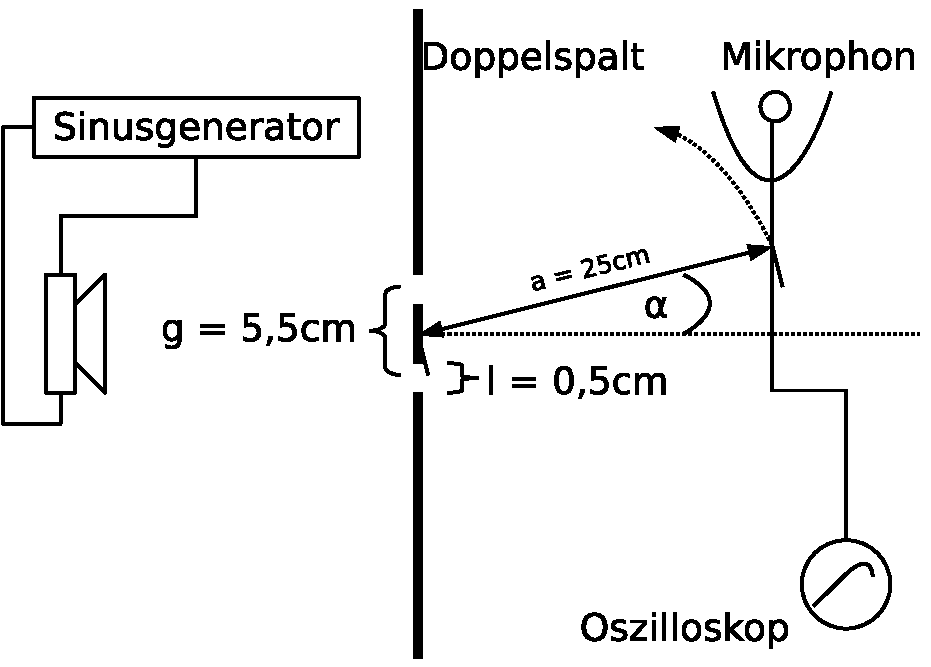
\includegraphics[width=0.8\textwidth]{praktika/mat_praktika/doppelspalt}
   \caption{Aufbau des Doppelspaltversuchs}
\end{figure}



Vor einen Doppelspalt aus Plastik wird eine Ultraschallsender in ca. \(20cm\) Abstand zwischen den beiden Spalten positioniert. Dies dient dazu, dass die Schallwellen, die auf die Spalte treffen eine feste Phasenbeziehung haben - steht der Sender genau zwischen den beiden Spalten (das wäre der Idealzustand), haben die Schallwellen, die von den Spalten ausgehen die Phasendifferenz \(\Delta \varphi = 0\).

Hinter dem Doppelspalt wird nun ein Mikrophon im Abstand von \(a = 25cm\)\footnote{Gemessen zum Mittelpunkt zwischen den beiden Spalten} halbkreisförmig bewegt\footnote{Dabei muss man sehr vorsichtig vorgehen, weil schon die Bewegung des Mikrophons zu Einer veränderten Anzeige führt; präzise Messungen können so nur bei \emph{ruhendem} Mikrophon vorgenommen werden.}. Über ein Oszilloskop wird überwacht, was das Mikrophon empfängt. Erkennt man auf dem Oszilloskop ein Minimum der vom Mikrophon registrierten Schallwellen\footnote{Eigentlich Minimum an registriertem \emph{Druck}; schließlich ist das Mikrophon druckempfindlich.}, so misst man den Winkel \(\alpha\) den der Lautsprecher zu einer gedachten Geraden senkrecht zum Doppelspalt durch den Mittelpunkt der Doppelspalte einschließt.

Dann gilt es, die Eigenfrequenz des Mikrophons zu ermitteln; offensichtlich nimmt es Frequenzen innerhalb eines kleinen Bereiches wesentlich besser war. Dazu wird das Mikrophon direkt vor den Lautsprecher gestellt und am Frequenzgenerator wird so lange de Frequenz verstellt, bis das Oszilloskop einen maximalen Ausschlag anzeigt. Bei uns ergab sich das für eine am Oszilloskop ablesbare Periodendauer von \(T = 24\mu s\); also bei einer Frequenz von \(f = \frac{1}{T} = 41 \frac{2}{3} kHz\). Über den Zusammenhang
\begin{equation}
   c = \frac{\lambda}{T} = \lambda \cdot f
   \label{eq_c=lf_p}
\end{equation}
ergab sich da \(c = 340 \frac{m}{s}\) eine Wellenlänge von \(\lambda \approx 8,16mm\).






\subsection{Beobachtungen}


``Lokale'' Maxima, bei denen der Ausschlag kleiner ist als in ihrer Umgebung, finden sich für folgende Winkel: 
\[ \alpha = \left \{   0^o; 11^o; 20^o; 27^o; 40^o; 50^o; 61^o  \right \} \]
Je größer der Winkel \(\alpha\) dabei ist, desto weniger Eindeutig ist das Maximum - also umso kleiner sind die im Oszilloskop beobachteten Wellenhöhen\footnote{Wellen, die man im Oszilloskop sieht}.


\subsection{Auswertung}


Maxima ergeben sich überall dort, wo der Gangunterschied der beiden von den Doppelspalten weglaufenden Wellen 
\begin{equation}
	\delta = k \cdot \lambda ~~ k = (0; 1; 2; ...)   
	\label{eq_gangunterschied}
\end{equation}
beträgt; an dieser Stelle haben die beiden Wellen, die von den Spalten ausgehen und sich zur gemessenen Welle addieren den Phasenunterschied \(\Delta \varphi = 0\); es gilt nämlich
\begin{equation} 
   \frac{\Delta \varphi}{2 \cdot \pi} = \frac{\delta}{\lambda}
   \label{eq_zshg_gangunterschied-phasendiffernz}
\end{equation} 
Im Zeigermodell addieren sich somit zwei parallele Zeiger zu einem resultierenden, der somit logischerweise die maximale durch Addition erreichbare Länge hat.


In unserem Versuch gilt der Zusammenhang \(a \gg g\) näherungsweise. Somit haben die im Mikrophon eintreffenden Schallwellen einen nahezu parallelen Weg zurückgelegt und somit kann man näherungsweise sagen, dass gilt:
\begin{equation}
   \delta = g \cdot sin( \alpha )
   \label{eq_fraunhofer_gangunterschied}
\end{equation}
Da sich die Gangunterschiede, bei denen sich Maxima ergeben nach Formel \ref{eq_gangunterschied} berechnen lassen, kann man Formel \ref{eq_fraunhofer_gangunterschied} und Formel \ref{eq_gangunterschied} kombinieren und es ergibt sich die sog. \textsc{Fraunhofer} Näherung (siehe Kap. \ref{fraunhofer_naehrung} auf S. \pageref{fraunhofer_naehrung}):
\begin{equation}
   g \cdot sin( \alpha ) = k \cdot \lambda \Rightarrow asin\left ( \frac{k \cdot \lambda}{g}\right )   ~~ k = (0; 1; 2; ...)   
\end{equation}
Danach ergeben sich für Maxima \(k\). Ordnung die Winkel in Tabelle \ref{tab_alpha_k} auf S. \pageref{tab_alpha_k}

\begin{table}
\centering
\begin{tabular}{l|l|l|l}
\(k\) &~~~ \(\alpha_k errechnet\) [\(^o\)] &~~~ \(\alpha_k gemessen\) [\(^o\)] &~~~ \(prozentuale Abweichung\) \\
\hline
0	&~~~	0	&~~~	0	&~~~	0\\
1	&~~~	8,53	&~~~	11	&~~~	-28,92\\
2	&~~~	17,26	&~~~	20	&~~~	-15,87\\
3	&~~~	26,43	&~~~	27	&~~~	-2,16\\
4	&~~~	36,4	&~~~	40	&~~~	-9,88\\
5	&~~~	47,89	&~~~	50	&~~~	-4,41\\
6	&~~~	62,9	&~~~	61	&~~~	3,01\\
\end{tabular}
\caption{Vergleich gemessener und errechneter Werte für \(\alpha\)}
\label{tab_alpha_k}
\end{table}



Für die von uns gemessenen Winkel ergeben sich so bei den einzelnen Maxima die Wellenlängen in Tabelle \ref{tab_lambda_k} auf S. \pageref{tab_lambda_k}

\begin{table}
\centering
\begin{tabular}{l|l|l|l}
\(k\)	&~~~	\(\alpha_k gemessen\) [\(^o\)]	&~~~	\(\lambda_k errechnet\) [mm]	&~~~	\(Prozentuale Abweichung\)\\
\hline
1	&~~~	11	&~~~	10,49	&~~~	-28,61\\
2	&~~~	20	&~~~	9,41	&~~~	-15,26\\
3	&~~~	27	&~~~	8,32	&~~~	-2\\
4	&~~~	40	&~~~	8,84	&~~~	-8,31\\
5	&~~~	50	&~~~	8,43	&~~~	-3,27\\
6	&~~~	61	&~~~	8,02	&~~~	1,75\\
\end{tabular}
\caption{Vergleich gemessener und errechneter Werte für \(\lambda\)}
\label{tab_lambda_k}
\end{table}


Es ergeben sich also besonders für große Winkel eine große Übereinstimmung der gemessenen und errechneten Werte.


\subsection{Mögliche Erklärungen für die Abweichungen}
\label{kap_abw01}


 Möglichkeiten für die Abweichungen können sein:
\begin{description}
   \item[Winkel] Die Winkel mussten mit einem Geodreieck abgemessen werden und es war leider zu kurz, um die Punkte, zwischen denen gemessen werden musste zu erreichen. Es musste also mehr oder weniger geschätzt werden.
   
   \item[Bestimmung der Punkte] Es war nicht ganz klar, zwischen welchen Punkten der Winkel überhaupt zu messen war; schließlich hätte man den soliden Fuß des Mikrophons unsichtbar und durchlässig machen müssen, um ihn zu erreichen...
   
   \item[Bestimmung eines Maximums] Bei der Entscheidung, ob es sich an entsprechender Stelle um ein Maximum handelte oder nicht hatte man bei der Untersuchung viel eignende Ermessensspielraum, ob es sich an besagter Stelle sicher um ein Maximum handelte oder nicht.
   
   \item[Wellenlänge] Die Wellenlänge haben wir errechnet in dem wir die Periodendauer vom Oszilloskop abgelesen haben - hier sind falsche Ablesungen möglich - außerden haben wir die ``standardisierte'' Schallgeschwindigkeit \(c = 340\frac{m}{s} \) verwendet, die aber bei uns sicher nicht galt (schließlich ist sie temperaturabhängig).
   
   \item[Fraunhofer Näherung] Die \textsc{Fraunhofer}-Näherung gilt eigentlich nur für sehr große Abstände von Mikrophon und Doppelspalt; möglicherweise war der unsrige zu klein...
\end{description}



		\subsection{\textsc{Fraunhofer}-Näherung} 
		\label{fraunhofer_naehrung}
Gilt bei der Beugung am Doppelspalt
\begin{equation}
a \gg g\\
 	\label{eq_aggg_p}
 \end{equation}
 \begin{equation}
a \gg d_k
 	\label{eq_aggdk_p}
\end{equation}
so kann man sich einigen Rechenaufwand sparen. Durch Formel \ref{eq_aggg_p} ist nämlich der Winkel \(\alpha_k\) nicht nur unter der Linie vom Punkt zwischen den Spalten zum Punkt auf den Leuchtschirm und der Horizontalen zu finden sondern auch näherungsweise zwischen den beiden Lichtstrahlen und einer gedachten Waagerechten. Außerdem sind die beiden Lichtstrahlen dadurch praktisch parallel und (nur) deswegen kann man den Winkel \(\alpha_k\) direkt an den Spalten wiederfinden (S. Skizze in Abbildung \ref{img_beugungamdoppelspalt_p} auf Seite \pageref{img_beugungamdoppelspalt_p}). Dadurch ergibt sich ein ähnliches Dreieck\footnote{Der Winkel \(\alpha_k\) und ein rechter Winkel findet sich sowohl in den kleinen Dreieck am Doppelspalt (in der Skizze teilweise. fein gestrichelt und fett) als auch in dem Dreieck, mit dem \(\alpha_k\) bestimmt wird (in der Skizze gestrichelt).} und so kann man hier auch den Gangunterschied \(\delta\) wiederfinden (in der Skizze fett). Dadurch ergibt sich
\begin{equation}
 	\delta = g \cdot sin(\alpha_k)
 		\label{eq_gangunterschied_doppelspalt_p}
\end{equation}
Bei geraden Schirmen kann man nun noch weiter vereinfachen. Der Abstand \(d_k\) ist über den geometrischen Zusammenhang
\begin{equation}
 	\frac{d_k}{a} = tan(\alpha_k) \Rightarrow d_k = a \cdot tan(\alpha_k)
 		\label{eq_doppelspalttangens_p}
\end{equation}
gegeben. Für \emph{sehr kleine} Winkel \(\alpha_k\) gilt
\begin{equation}
 	sin(\alpha_k) \approx \alpha_k \approx tan(\alpha_k)
 		\label{eq_winkelnaehrung_p}
\end{equation}
Und diese kleinen Winkel werden erreicht, wenn \(a \gg d_k\) gilt. Stimmt das \emph{nicht}, so ist diese zweite Vereinfachung nicht zulässig. Gilt sie doch, so gilt weiter

Für ein Maximum \(k\). Ordnung gilt näherungsweise
\begin{equation}
 \delta = g \cdot \frac{d_k}{a} = k \cdot \lambda ~~~ k = (0; 1; 2; 3; \ldots)
\end{equation}
und dementsprechend gilt für ein Minimum \(k\). Ordnung
\begin{equation}
 \delta = g \cdot \frac{d_k}{a} = k \cdot \lambda - \frac{\lambda}{2} ~~~ k = (1; 2; 3; \ldots)
\end{equation}




 



\begin{figure}
 \centering
 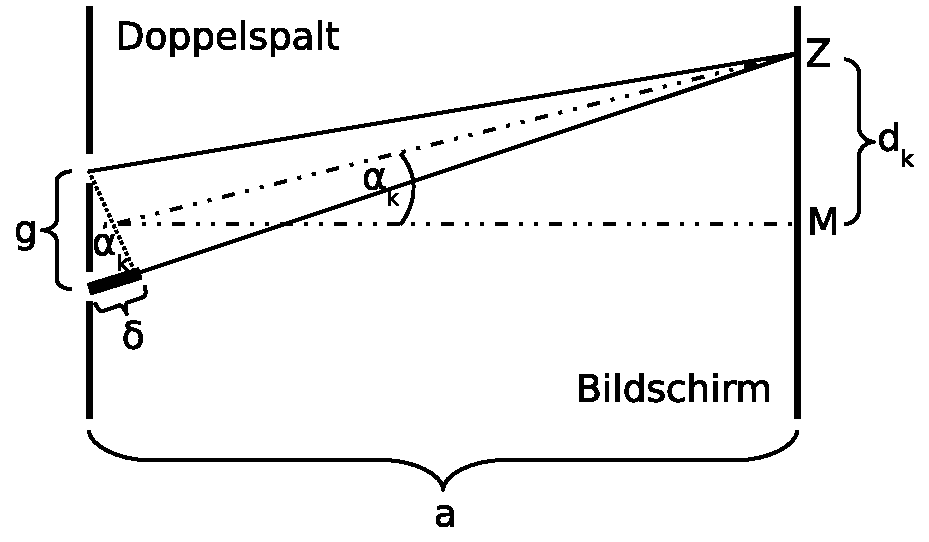
\includegraphics[width=0.7\textwidth]{praktika/mat_praktika/beugung_aufbau01}
 	\caption{Skizze zum Versuchsaufbau zur \emph{Beugung am Doppelspalt} bei geradem Bildschirm zur Erklärung der \textsc{Fraunhofer}-Näherung}
 		\label{img_beugungamdoppelspalt_p}
\end{figure}












\section{Reflektion an einer Halbdurchlässigen Lochplatte - A}


\subsection{Versuch}
\label{kap_reflexion01}

\begin{figure}
	\centering
   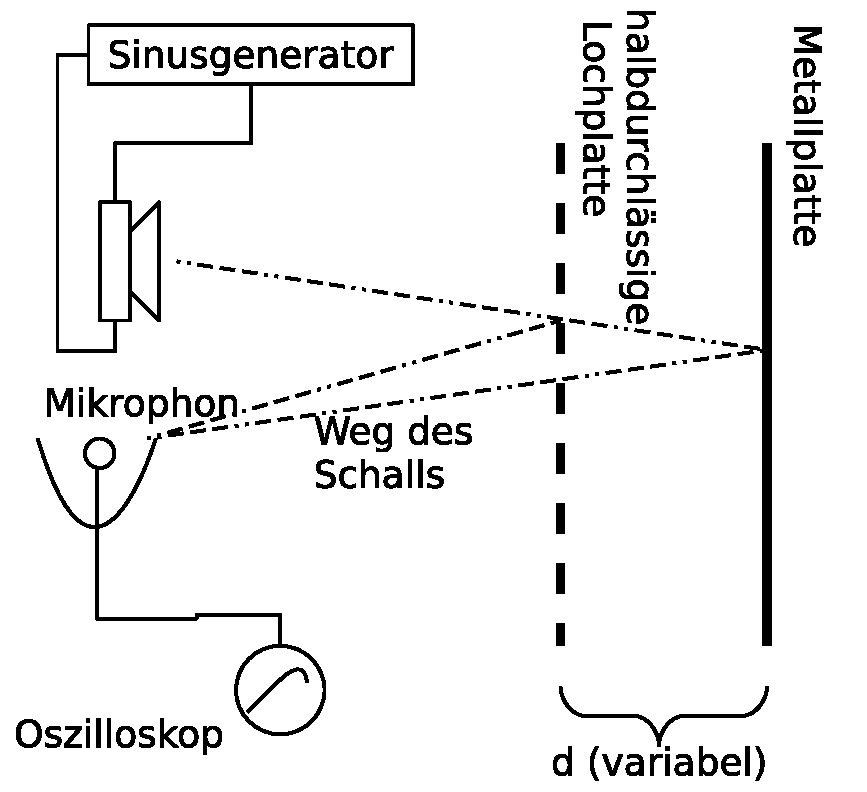
\includegraphics[width=0.6\textwidth]{praktika/mat_praktika/lochplatte}
   \caption{Aufbau des Versuchs über Reflexion an einer halbdurchlässigen Lochplatte.}
   \label{img_aufbau_lochplatte}
\end{figure}


Mikrophon und Lautsprecher werden nebeneinander vor eine Lochplatte gestellt, hinter der eine feste Metallplatte ist. Nun verschiebt man die feste Metallplatte in und entgegen der Richtung zur Lochplatte.




\subsection{Beobachtung}




Verschiebt man die feste Metallplatte in und entgegen der Richtung zur Lochplatte, so beobachtet man im Oszilloskop abwechselnd Minima und Maxima.

Bei unserem Aufbau ergaben sich Maxima bei Abständen \(d\) der Platten voneinander:
\[d = \left \{ 3,0cm; 3,75cm; 4,0cm; 4,7cm; 5,3cm; 5,8cm; 6,3cm; 6,8cm\right \}\]


Es ergeben sich dabei jedoch nie ``absolute'' Minima - also eine gerade Linie auf dem Oszilloskop.



\subsection{Auswertung}


Die Minima und Maxima ergaben sich durch Interferenz. In Abbildung \ref{img_aufbau_lochplatte} Sind die Wege des Schalls von Lautsprecher zu Empfänger eingezeichnet (gestrichelt). Der Schall wird also teilweise von der Lochplatte reflektiert und geht direkt weiter zum Mikrophon, teils kann der Schall aber auch durch die Lochplatte hindurch zur zweiten Wand von der er wieder reflektiert wird.\footnote{Beide Reflexionen erfolgen \emph{ohne} Phasensprung} Ein Teil dieses reflektierten Schalls kann durch die Löcher der Lochplatte wieder austreten. Diese Schallwellen addieren sich dann zu den direkt an der Lochplatte reflektierten. Haben diese beiden Schallwellen wenn sie beim Mikrophon eintreffen den Gangunterschied \(\delta = k \cdot \lambda ~~ k = (0; 1; 2; ...)\) so nimmt das Mikrophon ein Maximum war, bei einem Gangunterschied von \(\delta = k \cdot \lambda + \frac{\lambda}{2} ~~ k = (0; 1; 2; ...)\) registriert es ein Minimum.

Bei diesem Aufbau ist der Gangunterschied die Strecke, die der Schall zwischen Lochplatte und Metallplatte verbringt, somit kommt es auch auf den Abstand zwischen Empfänger und Lautsprecher und deren Abstand von der Lochplatte an, wie lange\footnote{also welche Strecke} der Schall zwischen den beiden Wänden Zeit verbringt\footnote{Je weiter Sender und Empfänger voneinander entfernt sind, desto größer wird der Reflexionswinkel und desto länger ist die Strecke des Schalls zwischen den Platten. Der selbe Effekt ergibt sich, wenn Sender und Empfänger näher bei den Platten sind.}. Da Lautsprecher und Empfänger aber sehr weit von den Platten entfernt sind, nahe beieinander stehen und die Löcher der Lochplatte sehr nahe aneinander liegen, kann man näherungsweise davon ausgehen, dass die Schallwellen senkrecht auf die Lochplatte fallen und ebenso senkrecht reflektiert werden. Somit darf man sagen, dass 
\begin{equation}
   \delta = 2 \cdot d
\end{equation}
näherungsweise gilt.\footnote{Der Schall muss den Abstand \(d\) doppelt überwinden (hin und zurück); daher die \(2\)}

Somit könnte man die Wellenlänge des Schalls über den Zusammenhang berechnen
\begin{equation}
  2 \cdot d = k \cdot \lambda ~~ k = (0; 1; 2; ...)
\end{equation}
Problematischerweise kann man über das \(k\) hierbei keine genauen Aussagen machen, weil man bedingt durch den Versuchsaufbau nicht \(d\) für \(k = 1\) einstellen kann (das wären \(4mm\) Abstand) geschweigedenn den Abstand \(d = 0\). Um zu erkennen, für welche \(k\) man also Maxima aufgezeichnet hat, wurden die Entsprechenden Wellenlängen ausgerechnet; dabei wurde unserem ersten Messwert (\(d = 3cm\)) \(k = k_0\) zugeordnet, dem nächsten Messwert \(k = k_0 + 1\) usw. Daraus wurden die jeweils resultierenden Wellenlängen berechnet und von diesen dann die Abweichung voneinander. Nun wurde der Wert \(k_0\) so lange verändert, bis die Abweichung der errechneten Wellenlängen minimal war; das ergab sich für \(k_0 = 9\).  In Tabelle \ref{tab_lochplatte_wellenlaenge} auf S. \pageref{tab_lochplatte_wellenlaenge} ist zusammengefasst, was sich für unsere Messwerte somit ergibt.


\begin{table}
\centering
\begin{tabular}{l|l|l|l}
\(k\)	&~~~	\(d\) [mm]	&~~~	\(\lambda\) [mm]	&~~~	\(prozentuale Abweichung\)\\
\hline
9	&~~~	30	&~~~	6,67	&~~~	18,3\\
10	&~~~	37,5	&~~~	7,5	&~~~	8,09\\
11	&~~~	40	&~~~	7,27	&~~~	10,87\\
12	&~~~	47	&~~~	7,83	&~~~	4\\
13	&~~~	53	&~~~	8,15	&~~~	0,08\\
14	&~~~	58	&~~~	8,29	&~~~	-1,54\\
15	&~~~	63	&~~~	8,4	&~~~	-2,94\\
16	&~~~	68	&~~~	8,5	&~~~	-4,17\end{tabular}
\caption{Aus unseren Verschiebungen \(d\) errechnete Wellenlängen und deren prozentuale Abweichung vom anfangs bestimmten Wert}
\label{tab_lochplatte_wellenlaenge}
\end{table}

Für \(k = 13\) wurde die Wellenlänge sehr genau bestimmt. Es ist hier ersichtlich, dass bei größeren Abständen \(d\) die Abweichung verhältnismäßig kleiner ist, als bei kleineren Abständen; ein kleiner Messfehler beim Abstand wird einerseits durch eine größere Zahl \(k\) geteilt und macht andererseits nur einen kleineren Prozentsatz von der gemessenen Länge aus. Außerdem fällt der verfälschende Anteil der Näherung geringer aus, je größer die Plattenabstände sind.


\subsection{Reflektionsanteil - A}
\label{kap_reflektionsanteil01}


Ein totales Minimum kann man nur dann beobachten, wenn die beim Mikrophon einlaufende Welle 
\begin{enumerate}
   \item[a)] einen Gangunterschied von \(\delta = \frac{\lambda}{2}\) hat und 
   \item[b)] genau die gleiche Amplitude.
\end{enumerate}

Reflektiert die Lochplatte \(40\%\) des Schalls direkt, so dürfte das vermutlich nicht reichen, damit sich ein absolutes Minimum bilden kann; schließlich werden von den \(60\%\), die die Lochplatte passieren nach der Reflexion nochmal \(40\%\) zur Metallplatte zurückgeworfen. Bei einer anfänglichen Intensität von \(I_0\) erreichen also \(0,4 \cdot I_0\) das Mikrophon direkt und \(0,6 \cdot 0,4 \cdot I_0 = 0,24 \cdot I_0\) erreichen das Mikrophon über eine einzige Reflektion an der Metallplatte; also nur etwas mehr als die Hälfte.

Was hierbei nicht einbezogen ist, sind
\begin{enumerate}
\sloppy   
   \item Der Schall verliert an Intensität, wenn er sich ausbreitet (reziprok kubisch). Da der Abstand \(2 \cdot d = \delta\), den der Schall auf seinem weiteren Weg zusätzlich  nehmen muss, verhältnismäßig klein ist, dürfte das nicht weiter ins Gewicht fallen.
   
   \item Möglicherweise ergeben sich zwischen Loch- und Metallplatte Interferenzphänomene (bspw. eine Stehende Welle), die dann mehr reflektieren kann wenn sie eine Weile angeregt wurde
   
   \item Der Schall, der einmal an der Metallwand reflektiert wurde und von der Lochplatte wieder zurückgeworfen wird, tritt nach einer erneuten Reflektion zu \(60\%\) wieder aus; es treten also \(0,6 \cdot 0,4 \cdot 0,6 \cdot I_0 = 0,114 \cdot I_0\) im nächsten ``Zyklus'' zusätzlich aus und somit tritt nach \(n\) ``Zyklen'' Die Intensität \(0,4^n \cdot 0,6^n \cdot I_0\) aus; Integriert man diese Funktion, so ergibt sich eine maximal austretende Intensität von ca. \(0,316 \cdot I_0\), somit also immer noch weniger als die reflektierten \(40\%\).
\end{enumerate}




\subsection{Mögliche Erklärungen für die Abweichung}
\label{kap_abw02}

Siehe hierzu auch Kap. \ref{kap_abw01} auf S. \pageref{kap_abw01}

\begin{description}
\sloppy
   \item[Wellenlänge] Möglicherweise wurde die Wellenlänge nicht präzise bestimmt; einmal durch Ablesefehler am Oszilloskop oder durch Verwendung der falschen Schallgeschwindigkeit
   
   \item[Abstand] Der Abstand wurde vermutlich nicht genau gemessen; schließlich kam es hierbei auf Millimeter an und man konnte ein Lineal nicht sinnvoll anlegen...
   
   \item[Maxima bestimmen] Es war nicht eindeutig, wann genau man ein Maxima antraf
   
   \item[Näherung] Es gilt bei den Werten zu bedenken, dass die errechneten Werte nur aus einer \emph{Nährungsformel} bestimmt wurden. Schließlich taucht in den Berechnungen weder der Abstand Mikrophon-Lautsprecher noch der Abstand Mikrophon-Lochplatte oder der Abstand der Löcher der Lochplatte auf. Möglicherweise würden unsere Messwerte mit einer präzieseren Berechnung exaktere Ergebnisse liefern.
   
   \item[Parallelität] Möglicherweise waren die beiden Platten nicht vollkommen parallel ausgerichtet oder waren uneben; so ergibt sich logischerweise unterschiedliche Abstände zwischen den Platten an verschiedenen Orgen.
\end{description}






\section{Reflekion an einer Halbdurchlässigen Lochplatte - B}



\subsection{Versuch}

\begin{figure}
	\centering
	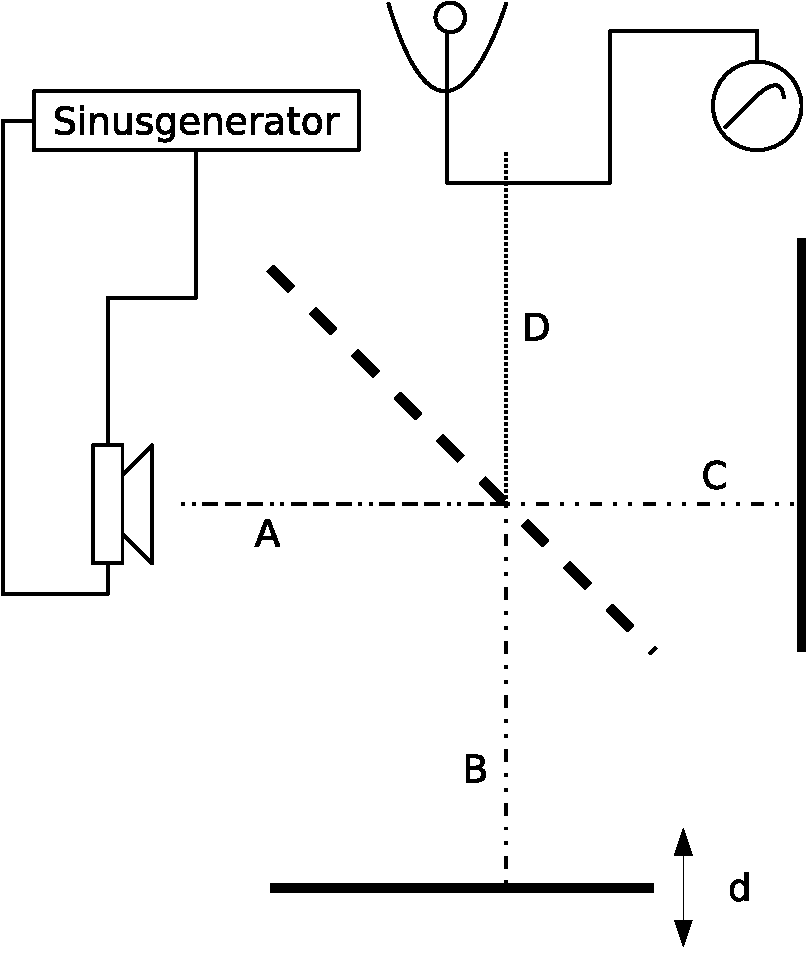
\includegraphics[width=0.5\textwidth]{praktika/mat_praktika/doppellochplatte}   
	\caption{Versuchsaufbau zur Bestimmung der Wellenlänge durch teilweise Refelxion an einer Lochplatte (Zur Zeichenerklärung siehe Abb. \ref{img_aufbau_lochplatte}, S. \pageref{img_aufbau_lochplatte})}
	\label{img_aufbau_doppellochplatte}
\end{figure}


Auf eine schräge Lochplatte werden Schallwellen geworfen. Sie werden teilweise nach unten\footnote{Richtungsangaben beziehen sich auf die Skizze in Abb. \ref{img_aufbau_doppellochplatte} auf S. \pageref{img_aufbau_doppellochplatte}} reflektiert, können auch teilweise nach rechts weiterlaufen. Sowohl unten als auch rechts stehen Metallplatten senkrecht zur Ausbreitungsrichtung des Schalls und reflektieren diesen. Über der Lochplatte befindet sich ein an ein Oszilloskop angeschlossenes Mikrophon, mit dem man die Intensität der Schallwellen\footnote{das Mikrophon ist druckempfindlich} bestimmen kann. Die Schallwellen die rechts reflektiert wurden können zum Mikrophon reflektiert werden, die Schallwellen von unten können die Lochplatte zum Mikrophon passieren. Eine der beiden Metallplatten (in unserem Aufbau die untere) lässt sich dabei parallel zur Schallausbreitungsrichtung verschieben. Immer wenn man am Oszilloskop ein Maximum erkennen kann, misst man, wie weit diese Platte verschoben wurde.



\subsection{Beobachtungen}

Es ergeben sich auf dem Oszilloskop abwechselnd Minima und Maxima; die Minima sind manchmal fast nur eine Gerade auf dem Oszilloskop.

Bei den Abständen \(d\) von einer beliebigen Ausgangslage erkennt man Maxima auf dem Schirm:
\[d = \left \{0mm; 6,5mm; 9mm; 12mm; 23mm; 25mm; 30mm; 37mm; 41mm; 46mm; 50mm \right \} \]





\subsection{Auswertung}


Die Maxima ergeben sich wieder bei einem Gangungerschied der Schallwellen von \(\delta = k \cdot \lambda ~~ k = (0; 1; 2; ..)\). Bei der Reflektion an der Lochplatte nimmt eine Schallwelle den Weg B\footnote{Bezogen auf die Skizze in Abb. \ref{img_aufbau_doppellochplatte} auf S. \pageref{img_aufbau_doppellochplatte}}, die andere den Weg C; vorher nehmen sie einhellig den Weg A. Nachdem die Schallwellen an den Metallplatten reflektiert wurden, nehmen sie nach anschließender Reflektion bzw. Passierung\footnote{Der Akt des Hindurchgelangens ohne Reflektion} der Lochplatte wieder einhellig den Weg D. Auf diesem kommt es nun zu Überlagerungen.

Den Gangunterschied kann man also berechnen, indem man jeweils das Doppelte der Strecken B und C voneinander abzieht\footnote{Das Doppelte deswegen, weil der Schall ja sowohl den Weg hin als auch zurück nehmen muss.}. In der Nullstellung (\(d = 0mm\)) ist dieser Gangunterschied offenslichtlich ein Ganzzahliges Vielfaches der Wellenlänge; welches Vielfache (\(k\)) ist dabei nicht von Bedeutung.

Wir mussten die Metallplatte durchschnittlich um \(d_1 = 4,33mm\) bewegen\footnote{Dabei sind die Werte in zwei Gruppen aufgeteilt; bis einschl. \(12mm\) und ab \(23mm\) - hier wurden offensichtlich einzelne Werte übersprungen}. Um den Faktor \(k\) um eins zu erhöhen wurde die Platte also durchschnittlich um \(4,33mm\) bewegt; somit haben wir durchschnittlich einen Gangunterschied von \(2 \cdot 4,33mm = 8,66mm\) erzeugt. Da wir immer von Maximum zu Maximum gemenssen haben, müsste dieser Gagnunterschied mit der Wellenlänge des Schalls übereinstimmen. 

In der Tat haben wir eine Abweichung von ca. \(-6,1\%\) zu verzeichnen.





\subsection{Mögliche Erklärungen für die Abweichung}

Siehe hierzu auch Kap. \ref{kap_abw01} auf S. \pageref{kap_abw01} und Kap. \ref{kap_abw02} auf S. \pageref{kap_abw02}.


\begin{description}
   \item[Neigung] Möglicherweise war die Lochplatte nicht genau im \(45^o\) Winkel zu den reflektierenden Platten geneigt.
 \end{description}




\subsection{Reflektionsanteil - B}

Vgl. Argumentation in Kap. \ref{kap_reflektionsanteil01} auf S. \pageref{kap_reflektionsanteil01}


Bei diesem Versuch wird von einer Ausgangsintensität \(I_0\) \(40\%\) nach unten reflektiert, von diesen \(40\%\) können \(60\%\) die Lochplatte passieren, der Rest wird in Richtung des Lautsprechers zurückgeworfen. Über die Untere Platte gelangen also \(0,4 \cdot 0,6 \cdot I_0 = 0,24 \cdot I_0\) an das Mikrophon.

Passiert der Schall anfangs die Lochplatte, so nehmen \(60\%\) davon den Weg C. Von diesen \(60\%\) werden anschließend \(40\%\) in Richtung des Mikrophons reflektiert. Über diese Platte gelangen also \(0,6 \cdot 0,4 \cdot I_0 = 0,24 \cdot I_0\) an das Mikrophon.

Da aus beiden ``Schallwegen'' die selbe Intensität (und damit der selbe Druck) ans Mikrophon gelangt, ist es möglich, dass sich bei einem Gangunterschied von \(\delta = k \cdot \lambda + \frac{\lambda}{2} ~~ k = (0; 1; 2; ...)\) die Wellen völlig auslöschen; es ergibt sich also ein absolutes Minimum.


Dieses Absolute Minimum ist mit dem Aufbau in Kap. \ref{kap_reflexion01} auf S. \pageref{kap_reflexion01} nicht erreichbar.


Es gilt jedoch zu beachten, dass folgender Aspekt \emph{nicht} berücksichtigt wurde:
\begin{itemize}
   \item Der Schall verliert bei seiner Ausbreitung an Intensität (reziprok kubisch). Ist also eine der beiden Strecken B oder C deutlich länger, so dürfte diese Abnahme schon dazu führen, dass sich kein absolutes Minimum mehr bilden kann.
\end{itemize}




% \begin{appendix}
% \section{Anhang}
%   \textbf{\textit{\large Berechnung der Abweichung}}
%     
%     Um die Abweichungen zu berechnen wurde folgende Formel verwendet: 
%       
% \begin{equation}
% 100 \cdot \frac{w_g - w_l}{w_l}
% \end{equation}
% 
% Dabei ist \(w_g\) der gemessene Wert und \(w_l\) der errechnete bzw. Literaturwert.
% 
% 
% \end{appendix}









%\end{document}


\chapter{Versuche zu Ultraschall II}
% \documentclass[a4paper]{article}
% \usepackage[ngerman]{babel}
% \usepackage[utf8]{inputenc}
% \usepackage[top=2.5cm,bottom=1.75cm,right=2cm,left=2.3cm]{geometry}
% \usepackage{wrapfig}
% \usepackage{floatflt}
% \usepackage{graphicx}
% \usepackage[colorlinks=true,linkcolor=black,bookmarksnumbered=true,breaklinks=true,pdfstartview=FitH]{hyperref}
% 
% \title{\textbf{Praktikum 10} \\ ~ \\Ultraschall II}
% 
% \author{Michael Kopp}
% 
% \date{25. Oktober 2007}
% 
% %2007-11-04 12:30
% 
% \begin{document}
% 
% 
% \maketitle


			\section{Interferenz zweier Ultraschallwellen}

		\subsection{Versuch}
\label{kap_interferenz_versuch}

\begin{figure}
   \centering
   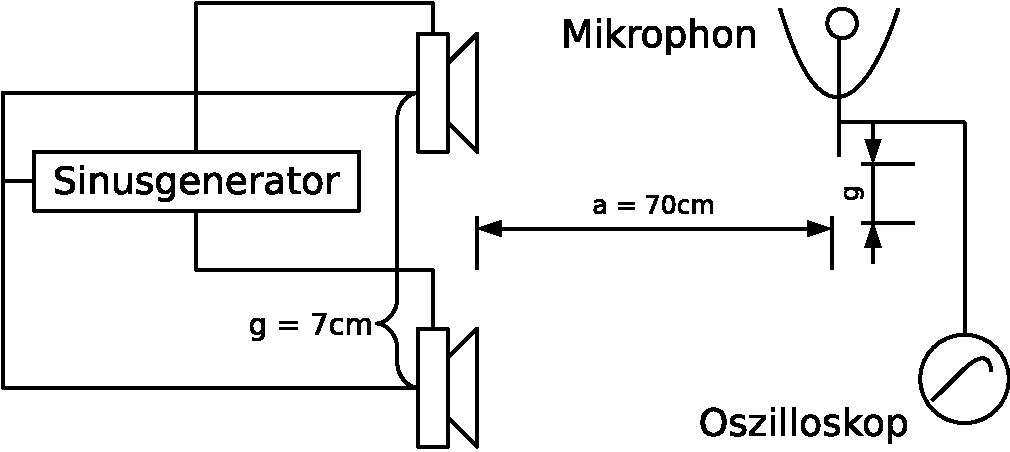
\includegraphics[width=0.8\textwidth]{praktika/mat_praktika/interferenz}
   \caption{Versuchsaufbau zum Interferenzversuch}
   \label{img_aufbau_interferenz}
\end{figure}


Zwei baugleiche Lautsprecher werden im Abstand \(g = 10cm\) voneinander parallel zueinander aufgestellt. Sie werden vom selben Sinusgenerator angesteuert und senden somit gleichphasige Schallwellen der gleichen Frequenz und Amplitude aus. Im Abstand \(a = 70cm\) senkrecht zur gedachten Verbindung der beiden Lautsprecher wird ein Mikrophon parallel zu der gedachten Verbindung um den Betrag \(g\) seitlich bewegt. Das Mikrophon ist druckempfindlich und auf einem Oszilloskop wird ausgegeben, welchen Druck es erfährt. (\(\rightarrow\) Abb. \ref{img_aufbau_interferenz}, S. \pageref{img_aufbau_interferenz})


Um die Wellenlänge des Ultraschalls zu ermitteln, stellt man das Mikrophon kurz vor einen der beiden Lautsprecher (der andere wird abgeschaltet) und verändert so lange die Frequenz am Sinusgenerator, bis die Amplitude auf dem Oszilloskop maximal wird. Auf dem Oszilloskop liest man die Periodendauer \(T = 24,4 \mu s\) ab. Somit beträgt die Frequenz \(f = \frac{1}{T} = 41kHz\). Über den Zusammenhang 
\begin{equation}
   c = \frac{\lambda}{T} = \lambda \cdot f
   \label{eq_c=lf}
\end{equation}
ergibt sich da \(c = 340 \frac{m}{s}\) eine Wellenlänge von \(\lambda \approx 8,30mm\).





		\subsection{Beobachtung}

Bewegt man das Mikrophon, so ergeben sich abwechselnd Minima und Maxima auf dem Oszilloskop. Maxima sind anzutreffen bei
\[d_{max} = \left \{ 0cm; 5,5cm; 11,5cm; 17,5cm \right \}\]
und Minima sind anzutreffen bei
\[d_{min} = \left \{ 3cm; 9cm; 15cm \right \}\]

Vertauscht man die Anschlüsse an einem der beiden Lautsprecher, so erhält man dort, wo vorher Maxima waren nun Minima und andersherum entsprechend.




		\subsection{Auswertung}

Siehe auch vorhergehendes Praktikum -- viele Rechnungen werden dort ausführlich erklärt und hier nur noch angewendet...


\subsubsection{Wellenlänge}
\label{kap_interferenz_auswertung_wellenlaenge}

Da \(a \gg g\) ist, darf man in diesem Fall die erste \textsc{Fraunhofer}-Näherung anwenden (siehe dazu Praktikum 9). Die zweite \textsc{Fraunhofer}-Näherung darf man jedoch nicht mehr anwenden, sich für große Abstände \(d\) Winkel über \(5^o\) ergeben:
\[
   \alpha = atan \left ( \frac{d}{a} \right ) = atan \left ( \frac{17,5}{70} \right ) \approx 14^o
\]
Man muss also für jeden Abstand \(d_k\) den Zugehörigen Winkel \(\alpha_k\) ausrechnen
\begin{equation}
   \alpha_k = atan \left ( \frac{d}{a} \right )
   \label{eq_alpha_k}
\end{equation}
und diesen dann in die Formel für den Gangunterschied \(\delta\) einsetzen
\begin{equation}
   \delta = g \cdot sin ( \alpha_k )
   \label{eq_delta_k}
\end{equation}
Über die Bedingungen für ein Maximum am betreffenden Punkt
\begin{equation}
   \delta = k \cdot \lambda ~~ k = (0; 1; 2; ...)
   \label{eq_bed_max}
\end{equation}
bzw. für ein Minimum
\begin{equation}
   \delta = k \cdot \lambda + \frac{\lambda}{2}~~ k = (0; 1; 2; ...)
   \label{eq_bed_min}
\end{equation}
kann man die Formeln zusammenfassen, indem man Formel \ref{eq_alpha_k} in Formel \ref{eq_delta_k} einsetzt, diese mit Formel \ref{eq_bed_max} bzw. Formel \ref{eq_bed_min} gleichsetzt und nach \(\lambda\) auflöst.

Für uns ergibt sich so für Maxima:
\begin{equation}
   \lambda_{k, max} = \frac{g \cdot sin \left ( atan \left ( \frac{d}{a} \right ) \right )}{k}
\end{equation}
und für Minima
\begin{equation}
   \lambda_{k, min} = \frac{g \cdot sin \left ( atan \left ( \frac{d}{a} \right ) \right )}{k + 0,5}
\end{equation}
Die Werte die sich nach der \textsc{Fraunhofer}-Näherung ergeben, werden in Tabelle \ref{tab_lambda_d_min} auf S. \pageref{tab_lambda_d_min} aufgeführt (für die Minima) und in Tabelle \ref{tab_lambda_d_max} auf S. \pageref{tab_lambda_d_max} (für die Maxima). 

Es ergibt sich eine schreckliche Abweichungen von \(71,68\%\). Erstaunlicherweise liegen jedoch die anderen Werte sehr nahe beieinander. Das lässt schließen, dass die allererste Messung (in Tabelle \ref{tab_lambda_d_min}) ein Ausrutscher ist. Schließlich wird die Wellenlänge bei diesem Verfahren \emph{ohne} den Ausrutscher im Mittel mit \(\lambda = 8,2mm\) berechnet (also eine Abweichung von \(-1,2\%\)) bei einer Varianz von lediglich \(V(\lambda) = 0,07mm^2\).

\begin{table}
\centering
\begin{tabular}{l|l|l|l|l|l}
\(k\)	&~~~	\(d\) [cm]	&~~~	\(\alpha\) [\(^o\)]	&~~~	\(\delta\) [cm]	&~~~	\(\lambda\) [cm]	&~~~	prozentuale Abweichung\\
\hline
0	&~~~	5	&~~~	4,09	&~~~	0,71	&~~~	1,42	&~~~	71,68\\
1	&~~~	9	&~~~	7,33	&~~~	1,28	&~~~	0,85	&~~~	2,43\\
2	&~~~	15	&~~~	12,09	&~~~	2,1	&~~~	0,84	&~~~	0,98
\end{tabular}
\caption{Berechnung der Wellenlänge aus den Werten für Minima}
\label{tab_lambda_d_min}
\end{table}


\begin{table}
\centering
\begin{tabular}{l|l|l|l|l|l}
\(k\)	&~~~	\(d\) [cm]	&~~~	\(\alpha\) [\(^o\)]	&~~~	\(\delta\) [cm]	&~~~	\(\lambda\) [cm]	&~~~	prozentuale Abweichung\\
\hline
0	&~~~	0	&~~~	0	&~~~	0	&~~~		&~~~	0\\
1	&~~~	5,5	&~~~	4,49	&~~~	0,78	&~~~	0,78	&~~~	-5,63\\
2	&~~~	11,5	&~~~	9,33	&~~~	1,62	&~~~	0,81	&~~~	-2,34\\
3	&~~~	17,5	&~~~	14,04	&~~~	2,43	&~~~	0,81	&~~~	-2,6
\end{tabular}
\caption{Berechnung der Wellenlänge aus den Werten für Maxima}
\label{tab_lambda_d_max}
\end{table}




\subsubsection{Vertauschung der Anschlüsse}


Als die beiden Anschlüsse vertauscht wurden kehrten sich Minima und Maxima um, weil die Sender nicht mehr in Phase schwangen (\(\Delta \varphi = 0\)), sondern genau gegenphasig (\(\Delta \varphi = \pi\)); schließlich wurde durch die umgedrehte Polung der Stromfluss in der Spule des Lautsprechers genau in die Gegenrichtung (bezogen sowohl auf den früheren Zustand als auch auf den anderen Lausprecher) erwirkt. Wo bei ehemaliger Polung also ein Magnetfeld so aufgebaut wurde, dass die Membran angezogen wurde wurde nun ein genau gegenläufiges Magnetfeld aufgebaut, welches die Membran abstieß und somit einen Überdruck anstatt eines Unterdrucks erzeugte.



Die Schallwelle eines der beiden Lautsprecher musste somit also die Strecke \(\frac{\lambda}{2}\) zusätzlich zurücklegen bis sie in Phase mit der gerade am anderen Lautsprecher ausgehenden Welle war.
 Die Wellen hatten also direkt bei der Erzeugung eine Phasendifferenz von \(\Delta \varphi = \pi\) und damit auf der Geraden mit stets dem selben Abstand zu beiden Lautsprechern (``MiSe'') stets einen Gangunterschied von \(\delta = \frac{\lambda}{2}\). 
Auf dieser Gerade lag somit stets ein Minimum. 
 Da zwischen einem registrierten Minimum und einem Maximum die Phasendifferenz sich stets verändert - und zwar von \(\Delta \varphi = \pi\) bis \(\Delta \varphi = 0\); also um genau \(\pi\) - hatten logischerweise die Punkte an denen vorher ein Minimum lag nun ein Maximum, weil die Phasendifferenz zwischen der MiSe und dem Vorherigen Minimum sich um \(\pi\) änderte; jetzt ebenso, und damit bei gegenphasig schwingenden Lautsprechern die Phasendifferenz auf (ein ganzzahliges Vielfaches von) \(2 \cdot \pi\) erhöht wurde, woraus wiederum ein Gangunterschied von \(\delta = 0\) resultierte, der für das Entstehen eines Maximums verantwortlich ist.  :-)
 
 
 
 



			\section{Radarfalleneffekt}

Eine Radarfalle misst auf diese Art die Geschwindigkeit von Verkehrsteilnehmern

		\subsection{Versuch}



\begin{figure}
   \centering
   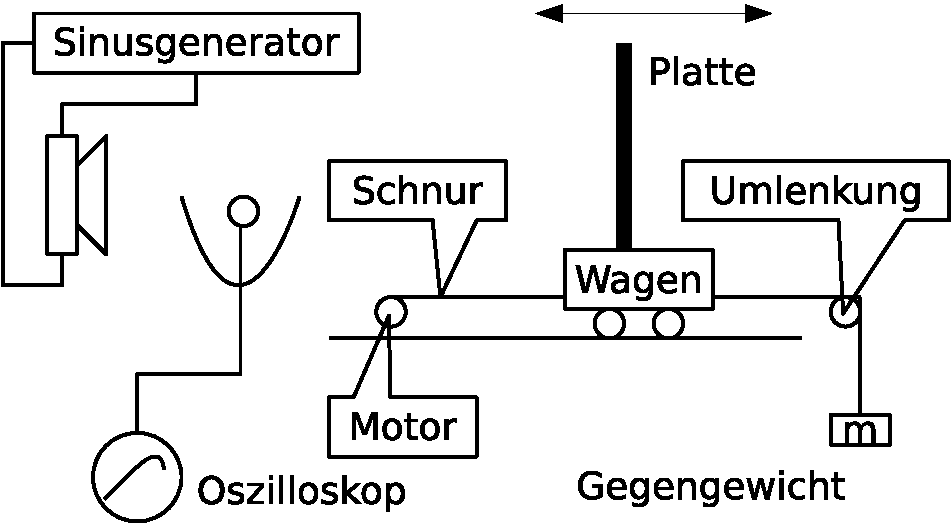
\includegraphics[width=0.8\textwidth]{praktika/mat_praktika/radar}
   \caption{Versuchsaufbau zum Versuch zum Radarfalleneffekt}
   \label{img_aufbau_radar}
\end{figure}



Auf einem Wagen, der mit der Geschwindigkeit \(v_0\) von einem Elektromotor bewegt wird, der mit einer konstanten Spannung von \(U = 0,4 V\) betrieben wird, ist eine Platte senkrecht zur Fahrtrichtung montiert. Hinter dem Wagen wird ein Lautsprecher aufgestellt und vor dem Lautsprecher ein Mikrophon, das an ein Oszilloskop gekoppelt ist.
Mit dem Oszilloskop wird gemessen, wie oft (\(n\)) in einer bestimmten Zeit \(t_0\) ein Druckbauch registriert wird.
(\(\rightarrow\) Abb. \ref{img_aufbau_radar}, S. \pageref{img_aufbau_radar})


Wie in Kapitel \ref{kap_interferenz_versuch} auf S. \pageref{kap_interferenz_versuch} muss zuerst wieder die Wellenlänge bestimmt werden. In diesem Falle ergibt sich eine Periodendauer von \(T = 8,75 \mu s\) und somit nach Formel \ref{eq_c=lf} die Wellenlänge \(\lambda = 5,95mm\).




		\subsection{Beobachtung}

Das Mikrophon registriert abwechselnd Druckminima und -maxima. In Tabelle \ref{tab_radarfalle_messwerte} auf S. \pageref{tab_radarfalle_messwerte} sind die Messwerte der verschiedenen Durchläufe festgehalten.


\begin{table}
\centering
   \begin{tabular}{c|c|c|c}
   	~~ \(t\) [sek] ~~ & ~~ \(n\) ~~ & ~~ \(v\) [\(\frac{mm}{s}\)] ~~ & ~~ prozentuale Abweichung ~~\\
   	\hline
   	37 & 68 & 5,47 & 4,3 \\
   	17 & 30 & 5,25 & -2,8 \\
   \end{tabular}
   \caption{Messwerte zum Versuch des Radarfalleneffekts}
   \label{tab_radarfalle_messwerte}

\end{table}





		\subsection{Auswertung}

Während sich der Wagen bewegt, ergibt sich ständig eine stehende Welle aus der zum Wagen hinlaufenden Welle und der vom Wagen reflektierten Welle. Dabei wird der Schalldruck an der Platte des Wagens stets ohne Phasensprung reflektiert und somit bildet sich an der Platte des Wagens stets ein Druckbauch. Von Druckbauch zu Druckbauch liegt der Abstand \(\frac{\lambda}{2}\). Zwischen den Druckbäuchen liegen Druckknoten, ebenfalls im Abstand \(\frac{\lambda}{2}\).

Misst man mit dem Oszilloskop in der Zeit \(t_0\) also \(n\) Druckknoten, so hat sich der Wagen dabei um \(s_0 = n \cdot \frac{\lambda}{2}\) bewegt, woraus sich die Geschwindigkeit 
\begin{equation}
   v_0 = \frac{s_0}{t_0} = \frac{n \cdot \frac{\lambda}{2}}{t_0} ~~~ [v_0] = \frac{mm}{s}
\end{equation}
errechnen lässt. Führt man diese Rechnung für unsere Messwerte durch, so erhält man die Ergebnisse, wie sie in Tabelle \ref{tab_radarfalle_messwerte} auf S. \pageref{tab_radarfalle_messwerte} aufgeführt sind.

festgehalten sind. Zur Kontrolle wurde die Geschwindigkeit ebenfalls bestimmt, indem die Zeit \(t_1\) gemessen wurde, die das Fahrzeug braucht, um de Strecke \(s_1 = 20cm\) zu überwinden. Demnach ist 
\[
   v_1 = \frac{s_1}{t_1} = \frac{20cm}{37sek} \approx 5,4 \frac{mm}{s}
\]
Die Abweichung unserer Werte ist ebenfalls in der Tabelle zu finden. Als Durchschnittswert für die aus unseren Messwerten berechnete Geschwindigkeit ergibt sich \(v_{0,durchschnitt} = 5,35 \frac{mm}{s}\), was mit einer Abweichung von \(-0,9\%\) als sehr präziese angesehen werden kann. 

Mögliche Ursachen für die Abweichung könnten sein:
 \begin{description}
    \item[verzählen bei Minima] Es ist bei dem Versuchsaufbau sehr einfach, dass man sich bei den Minima verzählt, weil sie so schnell auftraten und wieder verschwanden. 
    \item[Zeit stoppen] Außerdem musste man die Zeit, die der Wagen für die durchfahrenen \(20cm\) von Hand möglichst genau stoppen bzw. für das Durchlaufen der Minima, wobei ja immer reaktionsbedingte und augenmaßbedingte\footnote{Man konnte das Maßband nicht direkt an das Fahrzeug anlegen} Fehler einschleichen. 
    \item[Unregelmäßige Fahrt] Außerdem ist nicht auszuschließen, dass der Wagen nicht ganz regelmäßig auf der Schiene fuhr bzw. das Seil, welches sein Gegengewicht hielt nicht ganz regelmäßig durch die Halterung rutschte.
 \end{description}









			\section{Beugung am Gitter}



		\subsection{Versuch}


\begin{figure}
   \centering
   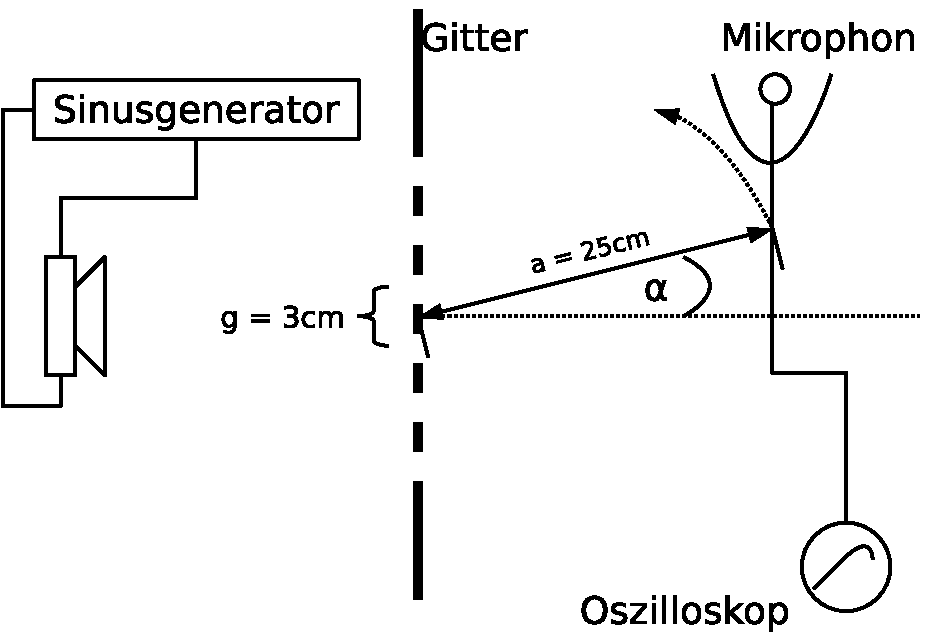
\includegraphics[width=0.8\textwidth]{praktika/mat_praktika/gitter}
   \caption{Versuchsaufbau zu Beugung am Gitter}
   \label{img_aufbau_gitter}
\end{figure}



Hinter einem Gitter mit der Gitterkonstanten \(g = 3cm\) wird ein Lautsprecher, der von einem Sinusgenerator betrieben wird, aufgestellt. In einem festen Abstand \(a = 25cm\) vom Gittermittelpunkt wird hinter dem Gitter ein Mikrophon halbkreisförmig bewegt. Das Mikrophon ist an ein Oszilloskop angeschlossen. Es registriert die Druckveränderungen. Erkennt man auf dem Oszilloskop ein Druckmaximum, so misst man den Winkel, den das Mikrophon von einer gedachten Senkrechten zum Gitter durch den Gittermittelpunkt überstrichen hat.
(\(\rightarrow\) Abb. \ref{img_aufbau_gitter}, S. \pageref{img_aufbau_gitter})

Beim bestimmen der Wellenlänge ergab sich eine Periodendauer von \(T = 21 \mu s\) und damit eine Wellenlänge von \(\lambda = 7,14mm\).



		\subsection{Beobachtungen}

In unserem Versuch ergaben sich Druckmaxima für 
\[
   \alpha_k = \left \{ 0^o; 12^o; 28^o; 58^o \right \}
\]




		\subsection{Auswertung}


Auch in diesem Falle darf man die erste \textsc{Fraunhofer}-Näherung anwenden (siehe Kap. \ref{kap_interferenz_auswertung_wellenlaenge} auf S. \pageref{kap_interferenz_auswertung_wellenlaenge}), da \(a \gg g\) gilt. Somit kann man die Wellenlänge berechnen, indem man Formel \ref{eq_delta_k} mit Formel \ref{eq_bed_max} gleichsetzt und nach \(\lambda\) auflöst:
\begin{equation}
   \lambda_k = \frac{g \cdot sin( \alpha_k )}{k}
\end{equation}
In Tabelle \ref{tab_gitter} auf S. \pageref{tab_gitter} sind die Ergebnisse der Rechnung mit der jeweiligen Abweichung von der Realität aufgeführt. Durchschnittlich ergibt sich bei unserer Messung eine Wellenlänge von \(\lambda_{durchschnitt} = 7,25mm\) bei einer Varianz von \(V(\lambda) = 1,29mm^2\) und so mit einer Standardabweichung von \(\sigma = 1,14mm\).

Gründe für die Abweichung können sein (vgl. und siehe Praktikum 9):
\begin{description}
   \item[Winkelmessen] Die Winkel mussten mit einem zu kurzen Geodreieck gemessen oder besser abgeschätzt werden
   \item[Punkte ausmachen] Es war nicht ohne weiteres möglich, die Punkte, zwischen denen die Winkel zu messen waren, auszumachen, weil dort, wo sie theoretisch sein müssten, das Stativmaterial war
   \item[Frequenz bestimmen] Die Frequenz bzw. Periodendauer zu bestimmen war nicht ganz einfach; es mussten wieder Striche auf dem Oszilloskop gezählt werden, aber manchmal war der Strahl auf dem Oszilloskop breiter aber auch so ließ sich die Periodendauer nicht besonders präzise ablesen, weil die Skala (die Markierungen auf dem Oszilloskop) zu groß gewählt war.
   \item[Maximum bestimmen] Es war nicht ganz einfach, eindeutig zu sagen, wann genau man das Maximum erreicht bzw. schon über- oder noch unterschritten hatte.
 \end{description}



\begin{table}
\centering
\begin{tabular}{l|l|l|l}
\(k\)	&~~~	\(\alpha\) [\(^o\)]	&~~~	\(\lambda\) [mm]	&~~~	prozentuale Abweichung\\
\hline
0	&~~~	0	&~~~	~	&~~~	0\\
1	&~~~	12	&~~~	6,24	&~~~	-12,64\\
2	&~~~	28	&~~~	7,04	&~~~	-1,37\\
3	&~~~	58	&~~~	8,48	&~~~	18,77
\end{tabular}
\caption{Berechnungen für die Wellenlänge bei Beugung am Gitter}
\label{tab_gitter}
\end{table}
















% \begin{appendix}
% 
% 				\section{Hinweise}
% 
% 		\subsection{Problem}
%    Unser Problem bei diesem Praktikum war, dass schlicht und ergreifend \emph{nichts} (keines der Experimente) in unserer Gruppe funktioniert hat; das Mikrophon hat von den beiden Lautsprechern unterschiedliche Frequenzen aufgezeichnet und hat man beide Lautsprecher gleichzeitig arbeiten lassen, ist das Signal völlig zusammengebrochen, betrieben wir nur ein Mikrophon, so durfte man den Abstand des Mikrophons nicht weiter verändern.
%    
%    	\subsection{Berechnung}
%    Um die Abweichungen zu berechnen wurde folgende Formel verwendet: 
% \begin{equation}
% 100 \cdot \frac{w_g - w_l}{w_l}
% \end{equation}
% Dabei ist \(w_g\) der gemessene Wert und \(w_l\) der errechnete bzw. Literaturwert.
% \end{appendix}








% 
% \end{document}


\chapter{Bestimmung des Planck'schen Wirkungsquantums}
% \documentclass[a4paper]{article}
% \usepackage[ngerman]{babel}
% \usepackage[utf8]{inputenc}
% \usepackage[top=2.5cm,bottom=1.75cm,right=2cm,left=2.3cm]{geometry}
% \usepackage{wrapfig}
% \usepackage{floatflt}
% \usepackage{subfigure}
% \usepackage{graphicx}
% \usepackage[colorlinks=true,linkcolor=black,bookmarksnumbered=true,breaklinks=true,pdfstartview=FitH]{hyperref}
% 
% \title{\textbf{Praktikum 12} \\ ~ \\Bestimmung des Planck'schen Wirkungsquantums}
% 
% \author{Michael Kopp}
% 
% \date{14. Februar 2008}
% 
% \begin{document}
% 
% \maketitle
% \tableofcontents



\section{Versuch}

Zur Bestimmung des \emph{\textsc{Planck}'schen Wirkungsquantums} $h$ benötigen wir die Wellenlänge $\lambda$ bzw. Frequenz $f$ untersuchten Lichts sowie die damit transportierte Energie $W$. Über den Zusammenhang $W = h \cdot f$ lässt sich dann das \textsc{Planck}'sche Wirkungsquantum errechnen:
\begin{equation}
   h = \frac{W}{f}
   \label{eq_hwf}
\end{equation}
Wir verwenden in unseren Versuchen Leuchtdioden. Einerseits weil ihr Licht weitgehend \emph{monochromatisch} ist, andererseits aber auch, weil die abgestrahlte Energie dabei leicht bestimmt werden kann.







\subsection{Bestimmung der Abgestrahlten Energie}

Bei Leuchtdioden muss jedes Elektron energetisch vom Valenzband auf ein Leitungsband angehoben werden. Von dort kann es wieder zurückfallen und bei diesem Zurückfallen ein Photon emittieren. Entscheidend ist dabei, dass ein Elektron eine bestimmte Mindestenergie braucht, um den \textit{Bandwechsel} vollziehen zu können. Diese Mindestenergie ist dann auch genau die Energie, die es wieder abgibt, wenn es vom energetisch höheren Leitungsband wieder in das Valenzband zurückfällt -- unabhängig davon, mit wie viel Energie \textit{hochgehievt} wurde.

Bestimmt man nun also die Energie, die zum Wechsel vom Valenz- ins Leitungsband von jedem Elektron aufgebracht werden muss, so ist diese Energie gleich der, die ein Elektron beim Übergang vom Leitungs- ins Valenzband in Form eines Photons abgibt. Wird an eine Diode die Spannung $U$ angelegt, so erhält ein einzelnes Elektron die Energie
\begin{equation}
   W = U \cdot e
   \label{eq_wue}
\end{equation}
Um nun die Energie zum Bandwechsel zu bestimmen, bestimmt man die \emph{kleinste mögliche} Spannung $U$, bei der Elektronen den Wechsel ins Leiterband schaffen. Dies äußert sich dann dadurch, dass die Diode überhaupt erst Strom leitet -- unterhalb dieser Spannung sitzen die Elektronen ja im Valenzband "`fest"'. Aus diesem Grund wird diese Spannung auch als \emph{Durchlassspannung} $U_D$ bezeichnet.

Praktisch verwendet man den in Abb. \ref{abb_schaltung} skizzierten Aufbau. Dabei wird eine Leuchtdiode über einen Widerstand in Durchlassrichtung mit einer regelbaren Spannungsquelle verbunden. Der fließende Strom wird gemessen ebenso wie die Spannung, die zwischen den Enden der Leuchtdiode -- und damit auch innerhalb der Leuchtdiode -- besteht. Die Spannung wird nun schrittweise erhöht und die Werte für Stromstärke und Spannung Tabelliert.


\begin{figure}
   \centering
   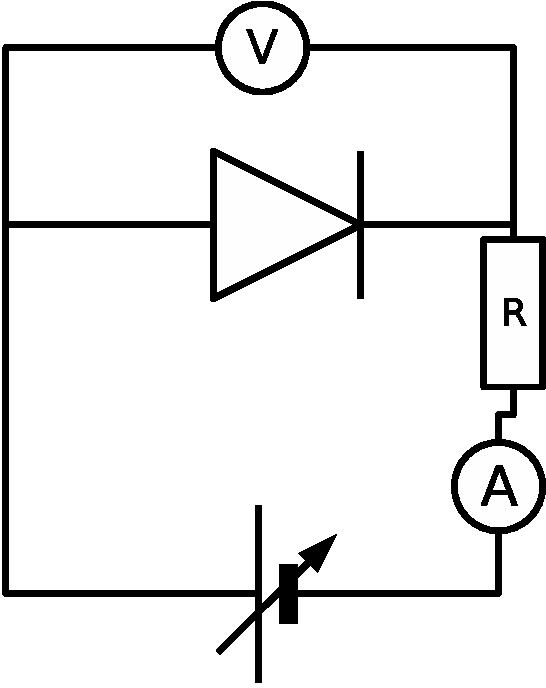
\includegraphics[width=0.4\textwidth]{praktika/mat_praktika/schaltung01}
   \caption{Aufbau um eine $I$-$U$-Kennlinie von Leuchtdioden aufzunehmen.}
   \label{abb_schaltung}
\end{figure}








\subsection{Bestimmung der Wellenlänge}

Zur Bestimmung der Wellenlänge von Licht verwendet man die Beugung von Licht am Gitter. Eine Leuchtdiode sendet als Lichtquelle Licht aus, welches in einem Gitter gebeugt wird. \emph{Hinter} dem Gitter steht ein Beobachter. Auf seine Netzhaut fällt das gebegte Licht. Nimmt das Auge ein Maximum wahr, so geht das Gehirn davon aus, dass das Licht des Maximums sich senkrecht zur Gitterebene ausgebreitet hat. Das Gehirn spiegelt dem Beobachter also vor, er sähe zwei erste Maxima links und rechts\footnote{Wenn die Gitterstriche senkrecht verlaufen.} der Lichtquelle. In Abb. \ref{abb_wellenlaenge} ist dies im unteren Teil zu sehen.

Um nun aber die Wellenlänge von Licht bestimmen zu können, benötigt man theoretisch ein Maximum bekannter Ordnung auf einem Schirm. Der Schrim ist in diesem Falle unser Gehirn. Unterhalb der LED wird eine Schiene befestigt, auf der Klammern rechts und links befestigt sind. Diese werden so gestellt, dass sie die Maxima 1. Ordnung seitlich "`berühren"'. So kann man den Abstand zwischen den beiden Maxima festhalten.

Als Distanz $a$ vom Gitter zum Schirm im klassischen Versuch wird in diesem Aufbau die Distanz $a_2$ vom Gitter zu der Schine mit den Klammern verwendet. Hier kann man den Abstand $d_1$ zwischen zwei Maxima 1. Ordnung abmessen -- der Abstand vom Maximum 0. Ordnung zu einem 1. Ordnung beträgt somit $\frac{d_1}{2}$. Dieses Licht wird also um den Winkel $\alpha_1$ gebeugt:
\begin{equation}
   \alpha_1 = arctan \left ( \frac{d_1}{a} \right )
\end{equation}
Bei Licht darf man die \emph{\textsc{Fraunhofer}'sche Näherung} anwenden, weil $a_2 \gg g$ gilt. Somit ergibt sich für ein Maximum 1. Ordnung unter den Winkel $\alpha_1$ die Wellenlänge
\begin{equation}
   \lambda = g \cdot sin ( \alpha_1 ) =  g \cdot sin \left ( arctan \left ( \frac{d_1}{a} \right ) \right ) 
   \label{eq_wellenlaenge_berechnen}
\end{equation}



\begin{figure}
   \centering
   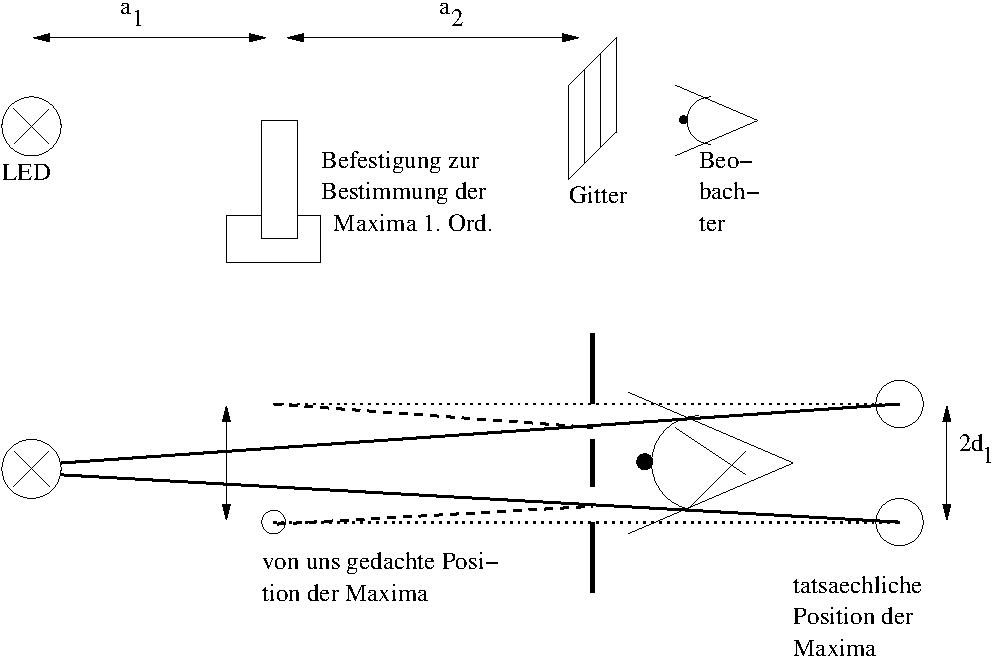
\includegraphics[width=\textwidth]{praktika/mat_praktika/aufbau_12}
   \caption{Versuchsaufbau zur Bestimmun der Wellenlänge von Licht}
   \label{abb_wellenlaenge}
\end{figure}






\section{Messwerte}


\subsection{Ermittlung der Durchschlagspannung}

Für verschiedene Leuchtdioden kamen wir auf die in Tabelle \ref{tab_messwerte} auf S. \pageref{tab_messwerte}zusammengestellten Ergebnisse. In Abb. \ref{abb_kennlinie} auf S. \pageref{abb_kennlinie} sind diese Werte zusammengefasst in Form von sog. \emph{I-U-Kennlinien}. In Tabelle \ref{tab_durchschlag} auf S. \pageref{tab_durchschlag} sind die einzelnen Durchschlagspannungen aufgelistet. %Die sich nach Formel \ref{eq_wue} ergebenden transportierten Energien sind hier ebenfalls eingetragen.


\begin{table}
\caption{Messwerte zur Bestimmung der Durchschlagspannung der einzelnen Leuchtdioden}\label{tab_messwerte}
\centering
\subtable[
Messwerte der blauen Leuchtdiode
]{
\begin{tabular}{l | l}
%~~~ # I  & ~~~ # U  \\
~~~ I [mA] & U [V]\\
\hline
~~~ 0  & ~~~ 0  \\
~~~ 0  & ~~~ 1.6  \\
~~~ 0.01  & ~~~ 1.64  \\
~~~ 1.18  & ~~~ 3.26  \\
~~~ 2.04  & ~~~ 3.34  \\
~~~ 2.98  & ~~~ 3.39  \\
~~~ 5.31  & ~~~ 3.47  \\
~~~ 6.92  & ~~~ 3.51  \\
~~~ 8.04  & ~~~ 3.54  \\
~~~ 10.18  & ~~~ 3.58  \\
~~~ 10.98  & ~~~ 3.59  \\
~~~ 12.05  & ~~~ 3.62  \\
~~~ 13.03  & ~~~ 3.63  \\
~~~ 13.51  & ~~~ 3.64  \\
~~~ 14.16  & ~~~ 3.65  \\
~~~ 15.02  & ~~~ 3.66  \\
~~~ 15.14  & ~~~ 3.66  \\
~~~ 17.37  & ~~~ 3.7  \\
\end{tabular}
}\label{tab_blau}
\subtable[
Messwerte der grünen Leuchtdiode
]{
\begin{tabular}{l | l}
%~~~ #I [mA]  & ~~~ U [V]  \\
~~~ I [mA] & ~~~~U [V]\\
\hline
~~~ 0  & ~~~ 0  \\
~~~ 0  & ~~~ 1.65  \\
~~~ 1.38  & ~~~ 1.85  \\
~~~ 3.31  & ~~~ 1.91  \\
~~~ 5.35  & ~~~ 1.96  \\
~~~ 7.5  & ~~~ 2  \\
~~~ 9.29  & ~~~ 2.03  \\
~~~ 10.6  & ~~~ 2.05  \\
~~~ 13.12  & ~~~ 2.09  \\
~~~ 14.7  & ~~~ 2.12  \\
~~~ 16.51  & ~~~ 2.14  \\
~~~ 18.5  & ~~~ 2.17  \\
\end{tabular}
}\label{tab_gruen}
\subtable[
Messwerte der gelben Leuchtdiode
]{
\begin{tabular}{l | l}
~~~ I [mA]  & ~~~ U [V]  \\
\hline
~~~ 0  & ~~~ 0  \\
~~~ 0  & ~~~ 1.52  \\
~~~ 0.1  & ~~~ 1.65  \\
~~~ 0.51  & ~~~ 1.71  \\
~~~ 1.66  & ~~~ 1.77  \\
~~~ 3.12  & ~~~ 1.82  \\
~~~ 3.35  & ~~~ 1.83  \\
~~~ 7.06  & ~~~ 1.91  \\
~~~ 7.94  & ~~~ 1.93  \\
~~~ 11.8  & ~~~ 2  \\
~~~ 15.03  & ~~~ 2.05  \\
~~~ 16.61  & ~~~ 1.98  \\
~~~ 19.8  & ~~~ 2.12  \\
\end{tabular}
}\label{tab_gelb}

\subtable[
Messwerte der roten Leuchtdiode
]{
\begin{tabular}{l | l}
~~~ I [mA]  & ~~~ U [V]  \\
\hline
~~~ 0  & ~~~ 0  \\
~~~ 0  & ~~~ 1.3  \\
~~~ 0.18  & ~~~ 1.46  \\
~~~ 1.43  & ~~~ 1.55  \\
~~~ 3.14  & ~~~ 1.58  \\
~~~ 7.16  & ~~~ 1.61  \\
~~~ 9.78  & ~~~ 1.62  \\
~~~ 11.75  & ~~~ 1.63  \\
~~~ 14.15  & ~~~ 1.64  \\
~~~ 16.25  & ~~~ 1.65  \\
~~~ 17.88  & ~~~ 1.65  \\
\end{tabular}
}\label{tab_rot}
\subtable[
Messwerte der infraroten Leuchtdiode
]{
\begin{tabular}{l | l}
~~~ I [mA]  & ~~~ U [V]  \\
\hline
~~~ 0  & ~~~ 0  \\
~~~ 0  & ~~~ 0.81  \\
~~~ 0.17  & ~~~ 0.95  \\
~~~ 0.67  & ~~~ 1.01  \\
~~~ 1.54  & ~~~ 1.04  \\
~~~ 2.57  & ~~~ 1.06  \\
~~~ 3.57  & ~~~ 1.08  \\
~~~ 5.71  & ~~~ 1.09  \\
~~~ 6.3  & ~~~ 1.1  \\
~~~ 8.18  & ~~~ 1.11  \\
~~~ 12.86  & ~~~ 1.13  \\
~~~ 13.95  & ~~~ 1.13  \\
~~~ 14.97  & ~~~ 1.14  \\
\end{tabular}
}\label{tab_ir}
\subtable[Durchschlagspannungen der einzelnen Leuchtdioden]{
\begin{tabular}{l l}
   Farbe der LED & $U_D$ [V]\\
   \hline
   Blau & 1,6  \\
   Grün  & 1,65\\
   Gelb & 1,52\\
   Rot & 1,3\\
   Infrarot & 0,81   \\
\end{tabular}\label{tab_durchschlag}}

\end{table}


\begin{figure}
   \centering
   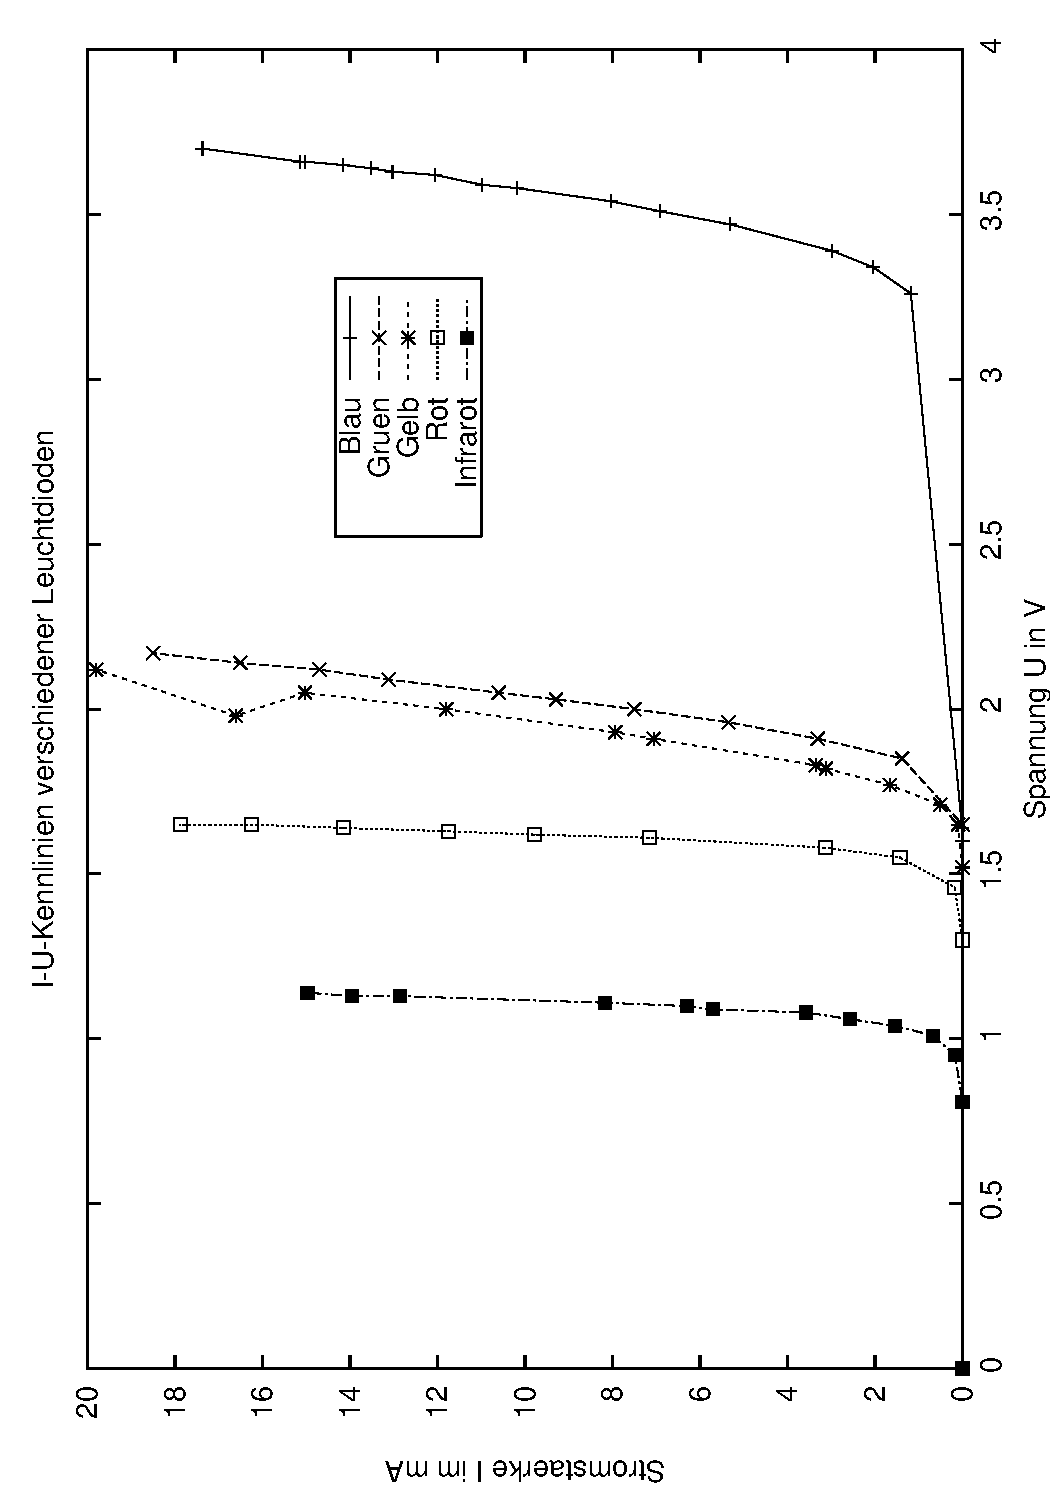
\includegraphics[height=\textwidth,angle=-90]{praktika/mat_praktika/plot01_01}
   \caption{Die Daten aus Tabelle \ref{tab_messwerte} in einem Schaubild zusammengefasst.}
   \label{abb_kennlinie}
\end{figure}








\subsection{Bestimmung der Wellenlänge}

Für unseren Aufbau gilt (nach Abb. \ref{abb_wellenlaenge}):

$a_2 = 0,80m = 80cm$

$g = 1 \cdot 10^{-5}$

Die Messwerte für die einzelnen Abstände sind in Tabelle \ref{tab_d_1} festgehalten.



\begin{table}[h]
   \centering
   \begin{tabular}{l l l}
   Farbe der LED & ~~~ $d_1$\\
   \hline
      Blau & ~~~ 8,6cm\\
      Grün & ~~~ 9,8cm\\
      Gelb & ~~~ 10,5cm\\
      Rot & ~~~ 11,4cm
   \end{tabular}
\caption{Messwerte zur Bestimmung der Wellenlänge der einzelnen LEDs}
\label{tab_d_1}
\end{table}







\section{Auswertung}

Für die einzelnen LEDs ergeben sich somit Energien (berechnet aus den Durchschlagspannungen aus Tab. \ref{tab_durchschlag} mit Gleichung \ref{eq_wue}) und Wellenlängen (berechnet aus der Lage der Maxima und Gleichung \ref{eq_wellenlaenge_berechnen}) wie sie in Tabelle \ref{tab_auswertung} festgehalten sind. Die Abweichung vom Literaturwert ist direkt dahinter angegeben -- für uns ergibt sich also eine Abweichung vom Literaturwert von durchschnittlich $-23,8\%$.




\begin{table}[h]
   \centering
   \begin{tabular}{l l l l l l}
      Farbe der LED & ~~~ $W$ [J]& ~~~ $\lambda$ [m]& ~~~ $f$ [Hz]& ~~~ $h$ [Js] & Abweichung\\
      \hline
      Blau & $2,56E-19$ & ~~~$5,37E-07$ & ~~~$5,59E+14$ & ~~~$4,59E-34$ & ~~~ $-3,08E-01$\\
      Grün & $2,64E-19$ & ~~~$6,11E-07$ & ~~~$4,91E+14$ & ~~~$5,39E-34$ & ~~~ $-1,88E-01$\\
      Gelb & $2,44E-19$ & ~~~$6,55E-07$ & ~~~$4,58E+14$ & ~~~$5,32E-34$ & ~~~ $-1,98E-01$\\
      Rot & $2,08E-19$ & ~~~$7,11E-07$ & ~~~$4,22E+14$ & ~~~$4,93E-34$ & ~~~ $-2,56E-01$
      
   \end{tabular}
   \caption{Die Messergebnisse aus der Bestimmung der abgestrahlten Energie und der Bestimmung der Wellenlänge werden hier zusammengesetzt und es wird das -- eigentlich gesuchte -- \textsc{Planck}'sche Wirkungsquantum errechnet.}
   \label{tab_auswertung}

\end{table}



\paragraph{Bestimmung von h näherungsweise aus einem f-D-Schaubild}


In Abb. \ref{abb_fu} auf S. \pageref{abb_fu} ist ein $f$-$U_D$-Diagramm für alle LEDs gezeichnet. Hier ist die Ablösespannung, die ja proportional zur Energie des Lichts ist über der Frequenz aufgetragen. Die Steigung ($m = \frac{\Delta y}{\Delta x}$) sollte nun eigentlich das \textsc{Planck}'sche Wirkungsquantum widergeben. Für die ersten drei Datenpunkte (der 4. wird als Ausreißer eingestuft) ergab sich $m = 0,508816$ und somit für $\Delta x = 100 \cdot 10^{14}$ $\Delta y = 0,508816 \cdot 100 \cdot 10^{14} = 5,08816 \cdot 10^{16}$. Somit ergibt sich für $h = 0,508816 \frac{eV}{100THz} = 8,15 \cdot 10^{-34} Js$ und damit eine Abweichung von $22,9\%$.



\begin{figure}
   \centering
   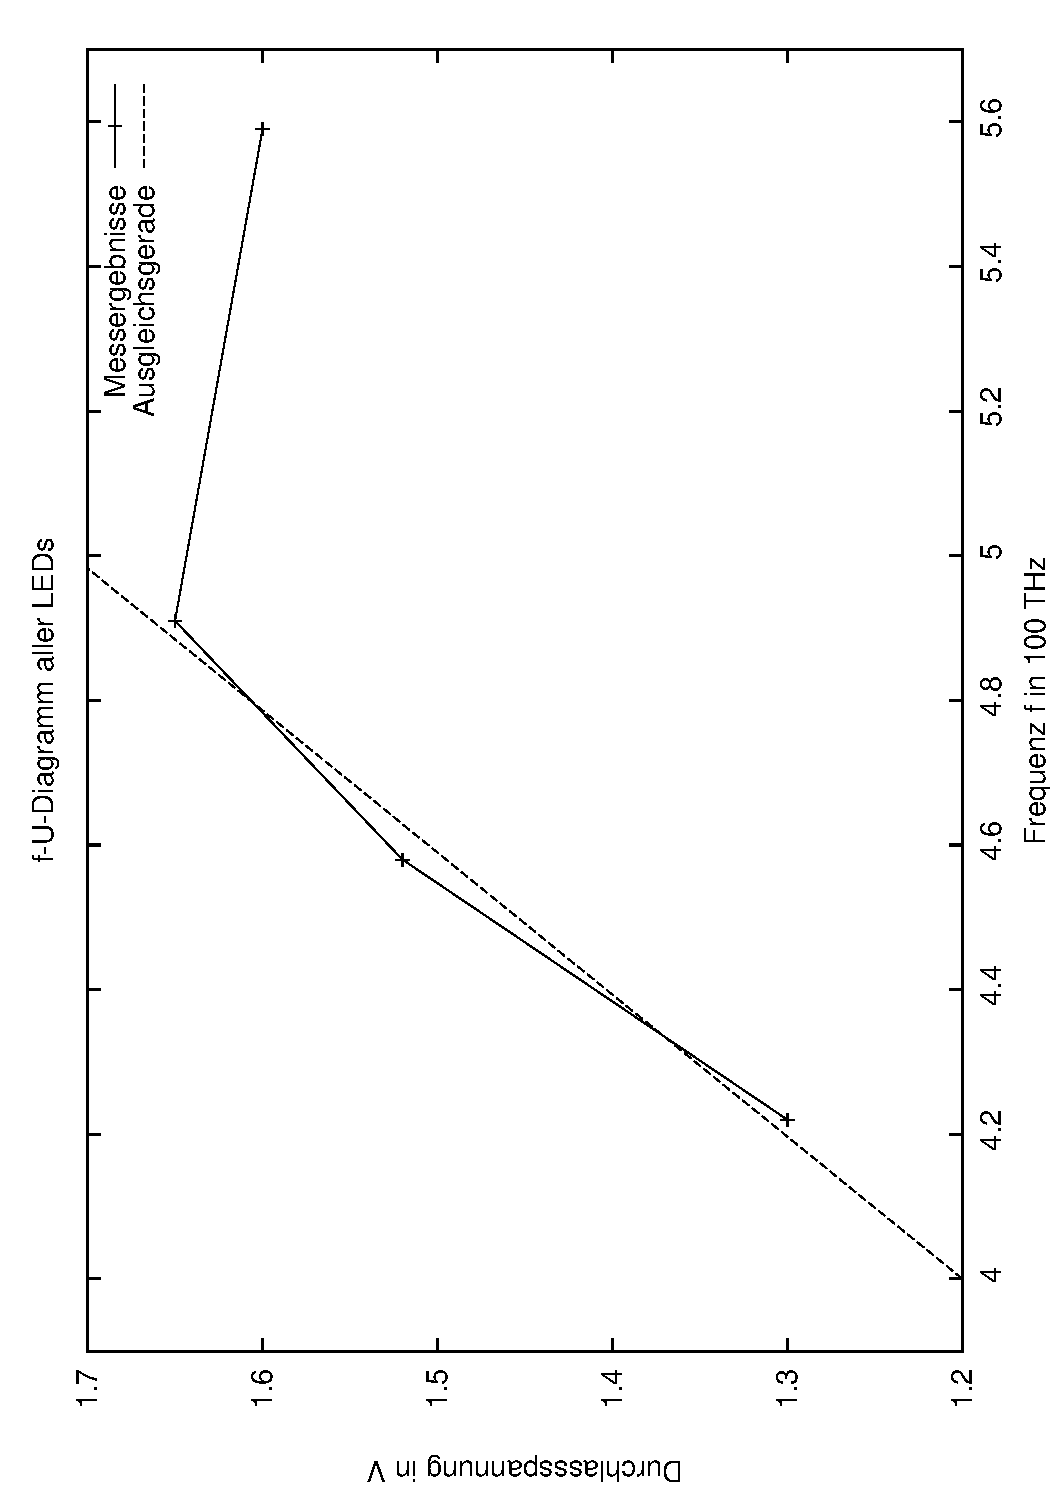
\includegraphics[height=\textwidth,angle=-90]{praktika/mat_praktika/fu_plot01}
   \caption{Ein $f$-$U_D$-Diagramm der LEDs}
   \label{abb_fu}
\end{figure}



\subsection{Fehlerquellen}



\begin{itemize}
   \item Vermutlich haben wir einfach die Distanz vom Gitter zum "`Schirm"' falsch bestimmt: Bspw. ergibt sich für $a_2 = 120cm$ eine durchschnittliche Abweichung von $1,51\%$.
   \item Dadurch dass wir digitale Messinstrumente vewendet haben, könnte es gut sein, dass bei einer bestimmten Spannung schon ein Strom floss, dieser aber nicht angezeigt werden konnte, weil die Zahl so klein war, dass sie hinter dem Komma "`verschwand"' -- dass wir diesen Strom also schlicht nicht ablesen konnten
   \item Das Licht der LEDs ist keinesfalls völlig monochromatisch -- das Maximum hatte schon einen "`Regenbogenrand"' der auf Zerlegung mehrerer Farben hindeutet. Den Abstand der Maxima so zu bestimmen war nicht ganz einfach.
   \item Beim Festsetzen der Klammern zum Markieren der einzelnen Maxima war ein Versuchsteilnehmer auf den anderen angewiesen: Einer beobachtete und dirigierte, der andere stellte ein. Verrutschte der Beobachter, so wurde die Messung zunehmend ungenau, weil sich so auch die Punkte der subjektiv wahrgenommenen Maxima verschoben.
   \item Bei dem Aufbau verrutschte Der Ständer der Diode beim wechseln der einzelnen Dioden -- die Abstände sind weniger genau
   \item Zur Bestimmung verwenden wir eine Näherung (erste \textsc{Fraunhofer}'sche Näherung) -- deswegen können unsere Versuchsergebnisse nicht völlig korrekt sein
   \item Widerstände in den Leitern verfälschen die Spannungsmessung: An der Sperrschicht in der Diode fällt weniger Spannung ab, als wir messen.

\end{itemize}




%\begin{appendix}

\section{Leuchtdioden, Photodioden \& Photozellen}


\paragraph{Leuchtdiode}

Eine Leuchtdiode [...] ist ein elektronisches Halbleiter-Bauelement. Fließt durch die Diode Strom in Durchlassrichtung, so strahlt sie Licht, Infrarotstrahlung oder auch Ultraviolettstrahlung mit einer vom Halbleitermaterial abhängigen Wellenlänge ab. [...]

Der Halbleiter einer LED bildet eine Diode. Durch Anlegen einer Spannung in Durchlassrichtung wandern Elektronen zur Rekombinationsschicht am p-n-Übergang. Auf der n-dotierten Seite bevölkern sie das Leitungsband, um nach Überschreiten der Grenzfläche auf das energetisch günstigere p-dotierte Valenzband zu wechseln, sie rekombinieren mit den dort vorhandenen Löchern. Bei Silizium-Dioden erfolgt der Übergang strahlungslos durch Phononenanregung, indem das Gitter den Impuls der Teilchen aufnimmt. Der direkte Übergang bei Gallium-Arsenid (GaAs) geht mit der Aussendung eines Photons einher. Ein weiterer Ursprung der Photonen besteht in einer plasmonisch-polaronischen Wechselwirkung, die durch einen spinfreien Übergang direkt zur Emission eines Auger-Photoelektrons führt. Dieser Mechanismus spielt insbesondere bei excitonischer Emission in grünen GaP-Leuchtdioden eine Rolle.  --- Quelle: \textsc{Wikipedia}




\paragraph{Fotodiode}

Photodioden sind Halbleiter-Dioden, die sichtbares Licht, in manchen Ausführungen auch IR-, UV- oder Röntgenstrahlen, an einem p-n-Übergang oder pin-Übergang durch den Inneren Fotoeffekt in einen elektrischen Strom umwandeln. Sie werden unter anderem verwendet, um Licht in ein Spannungssignal umzusetzen, oder um mit Licht übertragene Informationen weiterverarbeiten zu können. [...]

Treffen Photonen auf das Material der Diode, so werden in der Raumladungszone Ladungsträger (Elektron-Loch-Paare) erzeugt, was zu einem Stromfluss führt, da die Ladungsträger durch die Diffusionsspannung in die jeweils entgegengesetzt dotierten Zonen wandern. Die Photonen müssen eine höhere Energie als die des Bandabstandes aufweisen, um diesen Effekt hervorzurufen (bei Silizium z. B. mehr als \(1,1 eV\)). Der Fotostrom ist über viele Größenordnungen linear zum Lichteinfall, wenn keine Sättigung eintritt. Im Idealfall trägt jedes Lichtquant, das eine Energie besitzt, die größer als die charakteristische Energielücke (Bandabstand) des Halbleiters ist, zum Stromfluss bei. Praktisch ist der Wert jedoch kleiner und wird als Quantenausbeute bezeichnet. Die Reaktionszeit ist bei geeigneter Beschaltung sehr kurz; sie kann bis herab zu Bruchteilen einer Nanosekunde betragen.
Auch bei Dunkelheit fließt ein temperaturabhängiger, kleiner Strom - der sog. Dunkelstrom (\(I_D\)). Die Dunkelstromkennlinie ist ein wichtiges Qualitätsmerkmal von Fotodioden.  --- Quelle: \textsc{Wikipedia}



\paragraph{Fotozelle}

Eine Fotozelle [...] ist ein Strahlungsdetektor. Sie zählt insofern zu den Elektronenröhren, als sich auch bei ihr in einem evakuierten Glasgefäß eine Anode und eine Kathode (Fotokathode) befinden.

Die Fotokathode besteht aus einem Metall (z.B. Caesium mit besonders geringer Austrittsarbeit), aus dem durch Licht Elektronen freigesetzt werden können (Äußerer Fotoelektrischer Effekt).
 

Ist zwischen Anode (+) und Kathode (-) eine Spannung angelegt, so werden die vom Licht freigesetzten Elektronen zur Anode hin beschleunigt, ein elektrischer Strom (Fotostrom) kann gemessen werden. Ist die angelegte Spannung klein, so ist der Fotostrom proportional zur angelegten Spannung, der Proportionalitätsfaktor hängt von der Belichtungsintensität ab. Dieser Fotostrom geht bei höheren Spannungen in eine Sättigung über, d.h. der Strom steigt bei weiterer Erhöhung der angelegten Spannung nicht weiter an. Dies liegt daran, dass bei geringen Spannungen die elektrische Feldstärke nicht ausreicht, um alle durch den Fotoeffekt an der Kathode austretenden Elektronen in Richtung Anode zu beschleunigen und damit zum Fotostrom beitragen zu lassen. Allerdings können natürlich nicht mehr Elektronen zwischen Kathode und Anode fließen als durch das Licht freigesetzt werden, weshalb die Sättigung auftritt. Auch wenn keine Spannungsquelle mit der Fotozelle verbunden ist, bildet sich zwischen Anode und Kathode bei Belichtung eine Spannung aus - die Anode lädt sich negativ auf. Diese Spannung ist proportional zur Frequenz des eingestrahlten Lichts und kann zur Ermittlung des Planckschen Wirkungsquantums genutzt werden.

Die Spannung bildet sich aus, weil das Licht (genügend hohe Frequenz und damit Energie vorausgesetzt) Elektronen aus der Fotokathode herausschlägt. Diese Elektronen besitzen eine Energie, die der Differenz zwischen Quantenergie des Lichtes und Austrittsarbeit des Elektrons aus dem Kathoden-Metall entspricht. Die freien Elektronen treffen (teilweise) auch auf die Anode und laden diese negativ auf. Dadurch bildet sich eine elektrische Spannung zwischen den Elektroden aus. Weitere Elektronen müssen nun das sich ausbildende elektrische Feld durchlaufen, um auf die Anode aufzutreffen, wozu sie Energie benötigen. Schließlich ist die Spannung so groß, dass die Energie der neu herausgelösten Elektronen nicht mehr ausreicht, die Platte zu erreichen - die Spannung bleibt konstant.  --- Quelle: \textsc{Wikipedia}









%\end{appendix}







% 
% 
% \end{document}




\part{Index}
 \chapter*{}
 \section*{}
 \subsection*{}
     \begin{description}
	\item[\(\varepsilon_0\)] Elektrische Feldkonstante \(\varepsilon_0 \approx 8,85 \cdot 10^{-12} \frac{C}{Vm}\)
	\item[\(\frac{q}{m}\)] bezeichnet die \textit{Spezifische Ladung} eines Teilchens. Für Elektronen gilt: \( \frac{e}{m}~=~1,7588~\cdot~10^{11}~\frac{C}{kg}\)
	\item[\(\mu_r\)] bezeichnet die \textit{Permeabilitätszahl}, die festlegt, um wie viel stärker das Magnetfeld wird, wenn man einen Materiekern einführt.
	\item[\(h\)] steht für das \textit{Planck'sche Wirkungsquantum}, welches für die Quantenphysik eine bedeutende Rolle spielt. \(h = 6,62606896(33) \cdot 10^{-34}\ Js = 4{,}13566733(10) \cdot 10^{-15} eVs\)
\end{description}



   \newcommand{\orgtheindex}{}
 \let\orgtheindex\theindex
 \let\orgendtheindex\endtheindex
 \def\theindex{%
	\def\twocolumn{\begin{multicols}{3}}%
	\def\onecolumn{}%
	\clearpage
	\orgtheindex
 }
 \def\endtheindex{%
	\end{multicols}%
	\orgendtheindex
	\clearpage
 }

% \begin{small}
% \printindex
% \end{small}

\begin{footnotesize}
\printindex
\end{footnotesize}

\end{appendix}


\end{document}
